% Options for packages loaded elsewhere
\PassOptionsToPackage{unicode}{hyperref}
\PassOptionsToPackage{hyphens}{url}
\PassOptionsToPackage{dvipsnames,svgnames,x11names}{xcolor}
%
\documentclass[
  letterpaper,
  DIV=11,
  numbers=noendperiod]{scrreprt}

\usepackage{amsmath,amssymb}
\usepackage{iftex}
\ifPDFTeX
  \usepackage[T1]{fontenc}
  \usepackage[utf8]{inputenc}
  \usepackage{textcomp} % provide euro and other symbols
\else % if luatex or xetex
  \usepackage{unicode-math}
  \defaultfontfeatures{Scale=MatchLowercase}
  \defaultfontfeatures[\rmfamily]{Ligatures=TeX,Scale=1}
\fi
\usepackage{lmodern}
\ifPDFTeX\else  
    % xetex/luatex font selection
\fi
% Use upquote if available, for straight quotes in verbatim environments
\IfFileExists{upquote.sty}{\usepackage{upquote}}{}
\IfFileExists{microtype.sty}{% use microtype if available
  \usepackage[]{microtype}
  \UseMicrotypeSet[protrusion]{basicmath} % disable protrusion for tt fonts
}{}
\makeatletter
\@ifundefined{KOMAClassName}{% if non-KOMA class
  \IfFileExists{parskip.sty}{%
    \usepackage{parskip}
  }{% else
    \setlength{\parindent}{0pt}
    \setlength{\parskip}{6pt plus 2pt minus 1pt}}
}{% if KOMA class
  \KOMAoptions{parskip=half}}
\makeatother
\usepackage{xcolor}
\ifLuaTeX
  \usepackage{luacolor}
  \usepackage[soul]{lua-ul}
\else
  \usepackage{soul}
  
\fi
\setlength{\emergencystretch}{3em} % prevent overfull lines
\setcounter{secnumdepth}{5}
% Make \paragraph and \subparagraph free-standing
\ifx\paragraph\undefined\else
  \let\oldparagraph\paragraph
  \renewcommand{\paragraph}[1]{\oldparagraph{#1}\mbox{}}
\fi
\ifx\subparagraph\undefined\else
  \let\oldsubparagraph\subparagraph
  \renewcommand{\subparagraph}[1]{\oldsubparagraph{#1}\mbox{}}
\fi


\providecommand{\tightlist}{%
  \setlength{\itemsep}{0pt}\setlength{\parskip}{0pt}}\usepackage{longtable,booktabs,array}
\usepackage{calc} % for calculating minipage widths
% Correct order of tables after \paragraph or \subparagraph
\usepackage{etoolbox}
\makeatletter
\patchcmd\longtable{\par}{\if@noskipsec\mbox{}\fi\par}{}{}
\makeatother
% Allow footnotes in longtable head/foot
\IfFileExists{footnotehyper.sty}{\usepackage{footnotehyper}}{\usepackage{footnote}}
\makesavenoteenv{longtable}
\usepackage{graphicx}
\makeatletter
\def\maxwidth{\ifdim\Gin@nat@width>\linewidth\linewidth\else\Gin@nat@width\fi}
\def\maxheight{\ifdim\Gin@nat@height>\textheight\textheight\else\Gin@nat@height\fi}
\makeatother
% Scale images if necessary, so that they will not overflow the page
% margins by default, and it is still possible to overwrite the defaults
% using explicit options in \includegraphics[width, height, ...]{}
\setkeys{Gin}{width=\maxwidth,height=\maxheight,keepaspectratio}
% Set default figure placement to htbp
\makeatletter
\def\fps@figure{htbp}
\makeatother

\KOMAoption{captions}{tableheading}
\makeatletter
\@ifpackageloaded{tcolorbox}{}{\usepackage[skins,breakable]{tcolorbox}}
\@ifpackageloaded{fontawesome5}{}{\usepackage{fontawesome5}}
\definecolor{quarto-callout-color}{HTML}{909090}
\definecolor{quarto-callout-note-color}{HTML}{0758E5}
\definecolor{quarto-callout-important-color}{HTML}{CC1914}
\definecolor{quarto-callout-warning-color}{HTML}{EB9113}
\definecolor{quarto-callout-tip-color}{HTML}{00A047}
\definecolor{quarto-callout-caution-color}{HTML}{FC5300}
\definecolor{quarto-callout-color-frame}{HTML}{acacac}
\definecolor{quarto-callout-note-color-frame}{HTML}{4582ec}
\definecolor{quarto-callout-important-color-frame}{HTML}{d9534f}
\definecolor{quarto-callout-warning-color-frame}{HTML}{f0ad4e}
\definecolor{quarto-callout-tip-color-frame}{HTML}{02b875}
\definecolor{quarto-callout-caution-color-frame}{HTML}{fd7e14}
\makeatother
\makeatletter
\@ifpackageloaded{bookmark}{}{\usepackage{bookmark}}
\makeatother
\makeatletter
\@ifpackageloaded{caption}{}{\usepackage{caption}}
\AtBeginDocument{%
\ifdefined\contentsname
  \renewcommand*\contentsname{Table of contents}
\else
  \newcommand\contentsname{Table of contents}
\fi
\ifdefined\listfigurename
  \renewcommand*\listfigurename{List of Figures}
\else
  \newcommand\listfigurename{List of Figures}
\fi
\ifdefined\listtablename
  \renewcommand*\listtablename{List of Tables}
\else
  \newcommand\listtablename{List of Tables}
\fi
\ifdefined\figurename
  \renewcommand*\figurename{Figure}
\else
  \newcommand\figurename{Figure}
\fi
\ifdefined\tablename
  \renewcommand*\tablename{Table}
\else
  \newcommand\tablename{Table}
\fi
}
\@ifpackageloaded{float}{}{\usepackage{float}}
\floatstyle{ruled}
\@ifundefined{c@chapter}{\newfloat{codelisting}{h}{lop}}{\newfloat{codelisting}{h}{lop}[chapter]}
\floatname{codelisting}{Listing}
\newcommand*\listoflistings{\listof{codelisting}{List of Listings}}
\makeatother
\makeatletter
\makeatother
\makeatletter
\@ifpackageloaded{caption}{}{\usepackage{caption}}
\@ifpackageloaded{subcaption}{}{\usepackage{subcaption}}
\makeatother
\ifLuaTeX
  \usepackage{selnolig}  % disable illegal ligatures
\fi
\usepackage{bookmark}

\IfFileExists{xurl.sty}{\usepackage{xurl}}{} % add URL line breaks if available
\urlstyle{same} % disable monospaced font for URLs
\hypersetup{
  pdftitle={GEOU9SP GIS Workbook},
  pdfauthor={Thiago Silva, Allan Audsley, Lindis Kipp},
  colorlinks=true,
  linkcolor={blue},
  filecolor={Maroon},
  citecolor={Blue},
  urlcolor={Blue},
  pdfcreator={LaTeX via pandoc}}

\title{GEOU9SP GIS Workbook}
\author{Thiago Silva, Allan Audsley, Lindis Kipp}
\date{2026-12-01}

\begin{document}
\maketitle

\renewcommand*\contentsname{Table of contents}
{
\hypersetup{linkcolor=}
\setcounter{tocdepth}{2}
\tableofcontents
}
\bookmarksetup{startatroot}

\chapter*{Welcome!}\label{welcome}
\addcontentsline{toc}{chapter}{Welcome!}

\markboth{Welcome!}{Welcome!}

This e-book was created as a lab companion for the \emph{GEOU9SP -
Geographic Information Systems} module at University of Stirling. It
contains all the practical exercises that will be covered throughout the
module.

This book is \textbf{not a replacement to Canvas}, so make sure you are
engaging with the material on Canvas on a weekly basis!

The content of this book is organised into sections, which will
correspond to the teaching weeks and practical lab sessions. You will
always see the main content in the center window, with a detailed menu
covering all entries in the book on the left, and a chapter-specific
table of contents on the right. The Canvas pages for each lab session
will always link to the corresponding chapter in this book.

If you have any questions follow the instructions on Canvas on how to
\href{}{contact the module coordinator}.

\href{https://stir-my.sharepoint.com/:f:/g/personal/ala2_stir_ac_uk/EsP4F6F1Cq9AmT49tSHyTeUByKL4zoPEdZ4zvwGnJZF68A?e=77wlDJ}{You
can download PDf versions of each week's material from here}

\part{Week 1 - Introduction}

In our first week, we will get acquainted to with basic GIS data
manipulation using the QGIS software.

\section*{ILOs covered}\label{ilos-covered}
\addcontentsline{toc}{section}{ILOs covered}

\markright{ILOs covered}

\begin{enumerate}
\def\labelenumi{\arabic{enumi}.}
\item
  Understand the structure of spatial data and choose appropriate data
  types and models for storing and representing it;
\item
  Obtain and assess the quality of spatial data from online and offline
  sources and produce new spatial data using computer and field methods;
\item
  Create map visualisations that adhere to cartographic principles and
  can be easily and unambiguously interpreted by the non-specialist
  public;
\end{enumerate}

\section*{What will you learn}\label{what-will-you-learn}
\addcontentsline{toc}{section}{What will you learn}

\markright{What will you learn}

For every week, we will list the main theoretical and practical learning
goals. Use these as a `checklist' to gauge your learning for each week.
If you don't feel confident you have learned any specific topic, then
revisit the week's material!

\subsection*{Theoretical knowledge for Week
1:}\label{theoretical-knowledge-for-week-1}
\addcontentsline{toc}{subsection}{Theoretical knowledge for Week 1:}

\begin{itemize}
\tightlist
\item
  What are Geomatics, GIS, Remote Sensing and associated terms and
  fields?
\item
  What is spatial data?
\item
  What is a datum?
\item
  What is a map projection?
\item
  What is a Coordinate Reference System?
\end{itemize}

\subsection*{Practical knowledge:}\label{practical-knowledge}
\addcontentsline{toc}{subsection}{Practical knowledge:}

Chapter~\ref{sec-exoverview}

\begin{itemize}
\tightlist
\item
  How to launch QGIS
\item
  How to load a spatial data file
\item
  How to navigate the main QGIS interface
\item
  How to identify features
\item
  How to do basic measurements
\item
  How to do basic styling of spatial data
\item
  How to enter the layout editor
\item
  How to make and export a simple map layout
\end{itemize}

Chapter~\ref{sec-excrs}

\begin{itemize}
\tightlist
\item
  How to check the Coordinate Reference System of a spatial file
\item
  How to set the CRS of a QGIS project
\item
  How to set the CRS of a spatial file when it is already known.
\item
  How to reproject(convert) a spatial file from one CRS to another
\item
  What are the main CRSs you should be familiar with.
\end{itemize}

\chapter{Lab 1: QGIS overview and file management}\label{sec-exoverview}

The purpose of this lab is to give you a first overview of what a proper
GIS workflow looks like, from start to end. As you progress on your
exercises the projects will become more complex, but the general
workflow will not change.

Developing proper project and file management habits from the start is
the \emph{best} thing you can do to succeed in GIS. Speaking as someone
who has been teaching and working with Geomatics for more than a decade,
poor file/project management is the underlying cause of at least 50\% of
the GIS problems you may encounter.

\section{Before you start!}\label{before-you-start}

\begin{enumerate}
\def\labelenumi{\arabic{enumi}.}
\item
  Go through the Week 1 preparatory session on Canvas, and watch the
  seminar recording if you have missed it.
\item
  Read
  \href{https://www.ordnancesurvey.co.uk/documents/resources/guide-to-nationalgrid.pdf}{this
  document} to understand how the British National Grid indexing system
  works.
\end{enumerate}

\section{Guided Exercise 1 - Managing and loading files}\label{GE1}

In this exercise, you will download some data, prepare a \emph{folder
structure} to organise the files in your GIS projects, then create a
QGIS project file and add some GIS data to it.

\subsection{Downloading the required
data}\label{downloading-the-required-data}

For this practical you will use the ``OS open road'' and ``OS Terrain 50
Digital Terrain Model'' spatial datasets, specifically for the
\textbf{NS89} tile of the Ordnance Survey British National Grid. (Read
about what these datasets are here:
\href{https://www.ordnancesurvey.co.uk/products/os-open-roads}{OS Open
Roads} ,
\href{https://www.ordnancesurvey.co.uk/products/os-terrain-50}{OS
Terrain 50}).

\begin{enumerate}
\def\labelenumi{(\arabic{enumi})}
\item
  Head to the \href{https://digimap.edina.ac.uk/}{Digimap} website, and
  if you haven't already, make sure you accept the user licenses for all
  datasets, as show on the instructions video available on Canvas.
\item
  Go the \texttt{Ordnance\ Survey} section of the site, and then pick
  the \texttt{View\ maps\ and\ download\ data} option on the right.
\item
  Following the steps shown on the instructions video, download the
  following datasets \emph{for the NS89 BNG tile only}:
\end{enumerate}

\begin{itemize}
\tightlist
\item
  OS Open Roads (under \emph{Vector Data}) - choose the \texttt{SHP}
  format
\item
  ``OS Terrain 50 Digital Terrain Model'' (\emph{NOT Terrain 5 and NOT
  Contours!}, under Land and Height Data) - choose the \texttt{ASC}
  format
\end{itemize}

If you have correctly searched for tile NS89 and checked the required
datasets, you will see a screen like this:

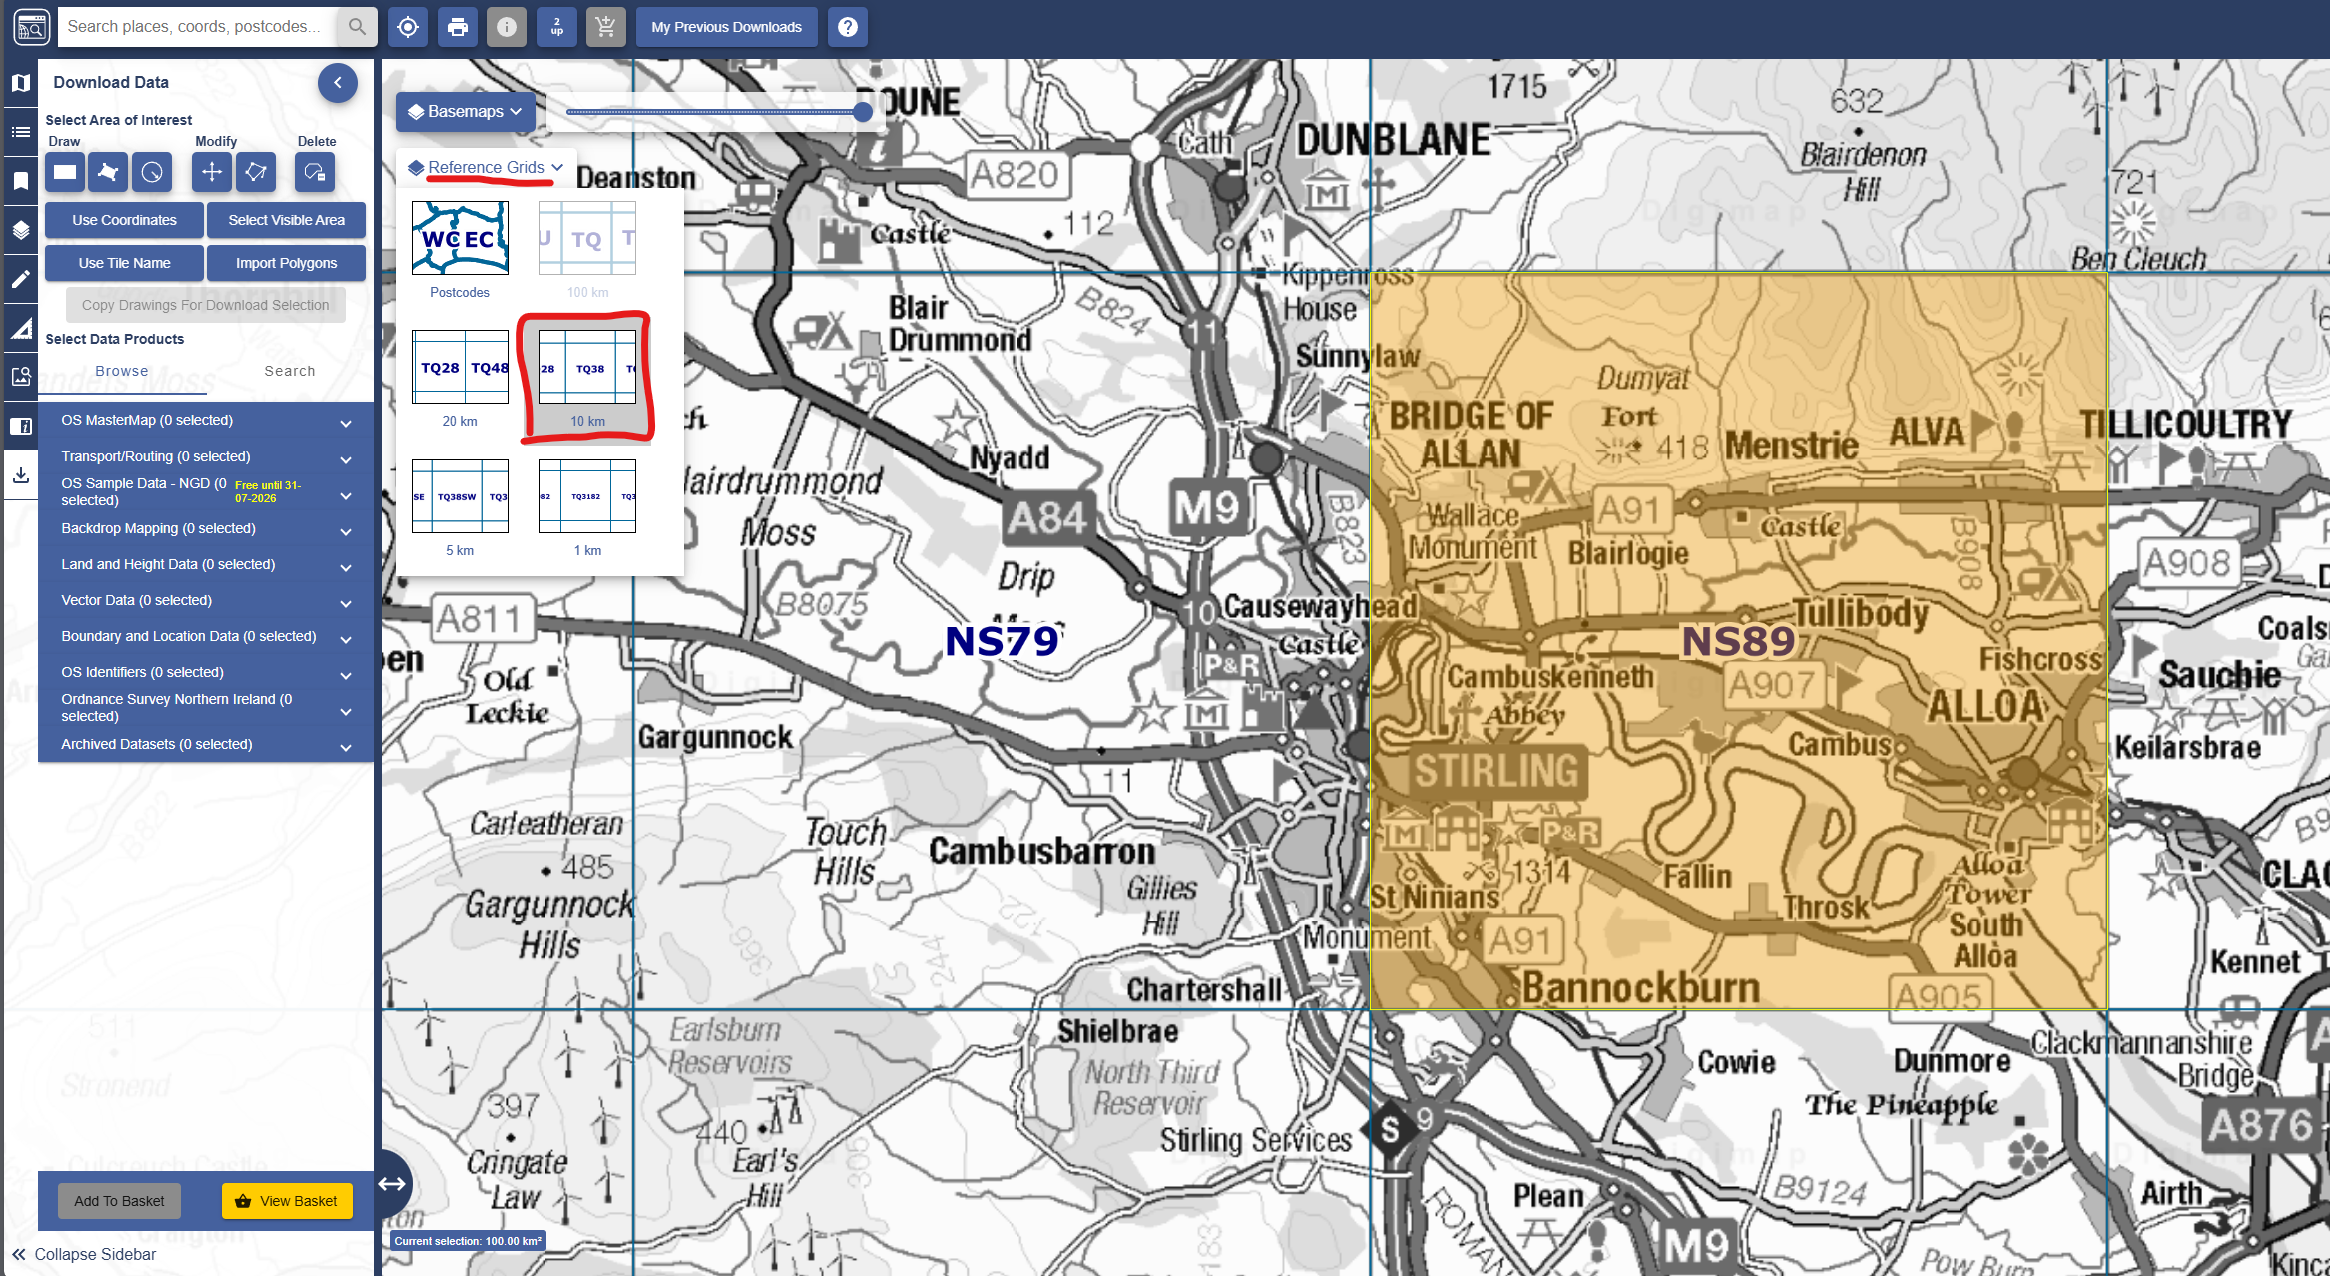
\includegraphics{images/lab_1/lab1_digimap.png}

\subsection{Creating a project
structure}\label{creating-a-project-structure}

GIS projects generate a lot of different files, and quickly, so project
organization is \textbf{essential}. The folder structure below is my
personal suggestion for organizing GIS projects files and associated
data. As you get comfortable managing your own projects, feel free to
change the organization structure to something that best suits your own
workflow and the specific project you are working on!

\begin{enumerate}
\def\labelenumi{(\arabic{enumi})}
\setcounter{enumi}{3}
\tightlist
\item
  Create a folder on your computer with the module name
  (\texttt{GEOU9SP}), off of your main work folder. For \textbf{Windows}
  this will usually be \texttt{Documents}. For \textbf{Linux} and
  \textbf{Mac}, create it on you \texttt{home} folder. (If you prefer
  and are comfortable with saving at another location on your computer,
  go for it!)
\end{enumerate}

\textbf{Windows:}

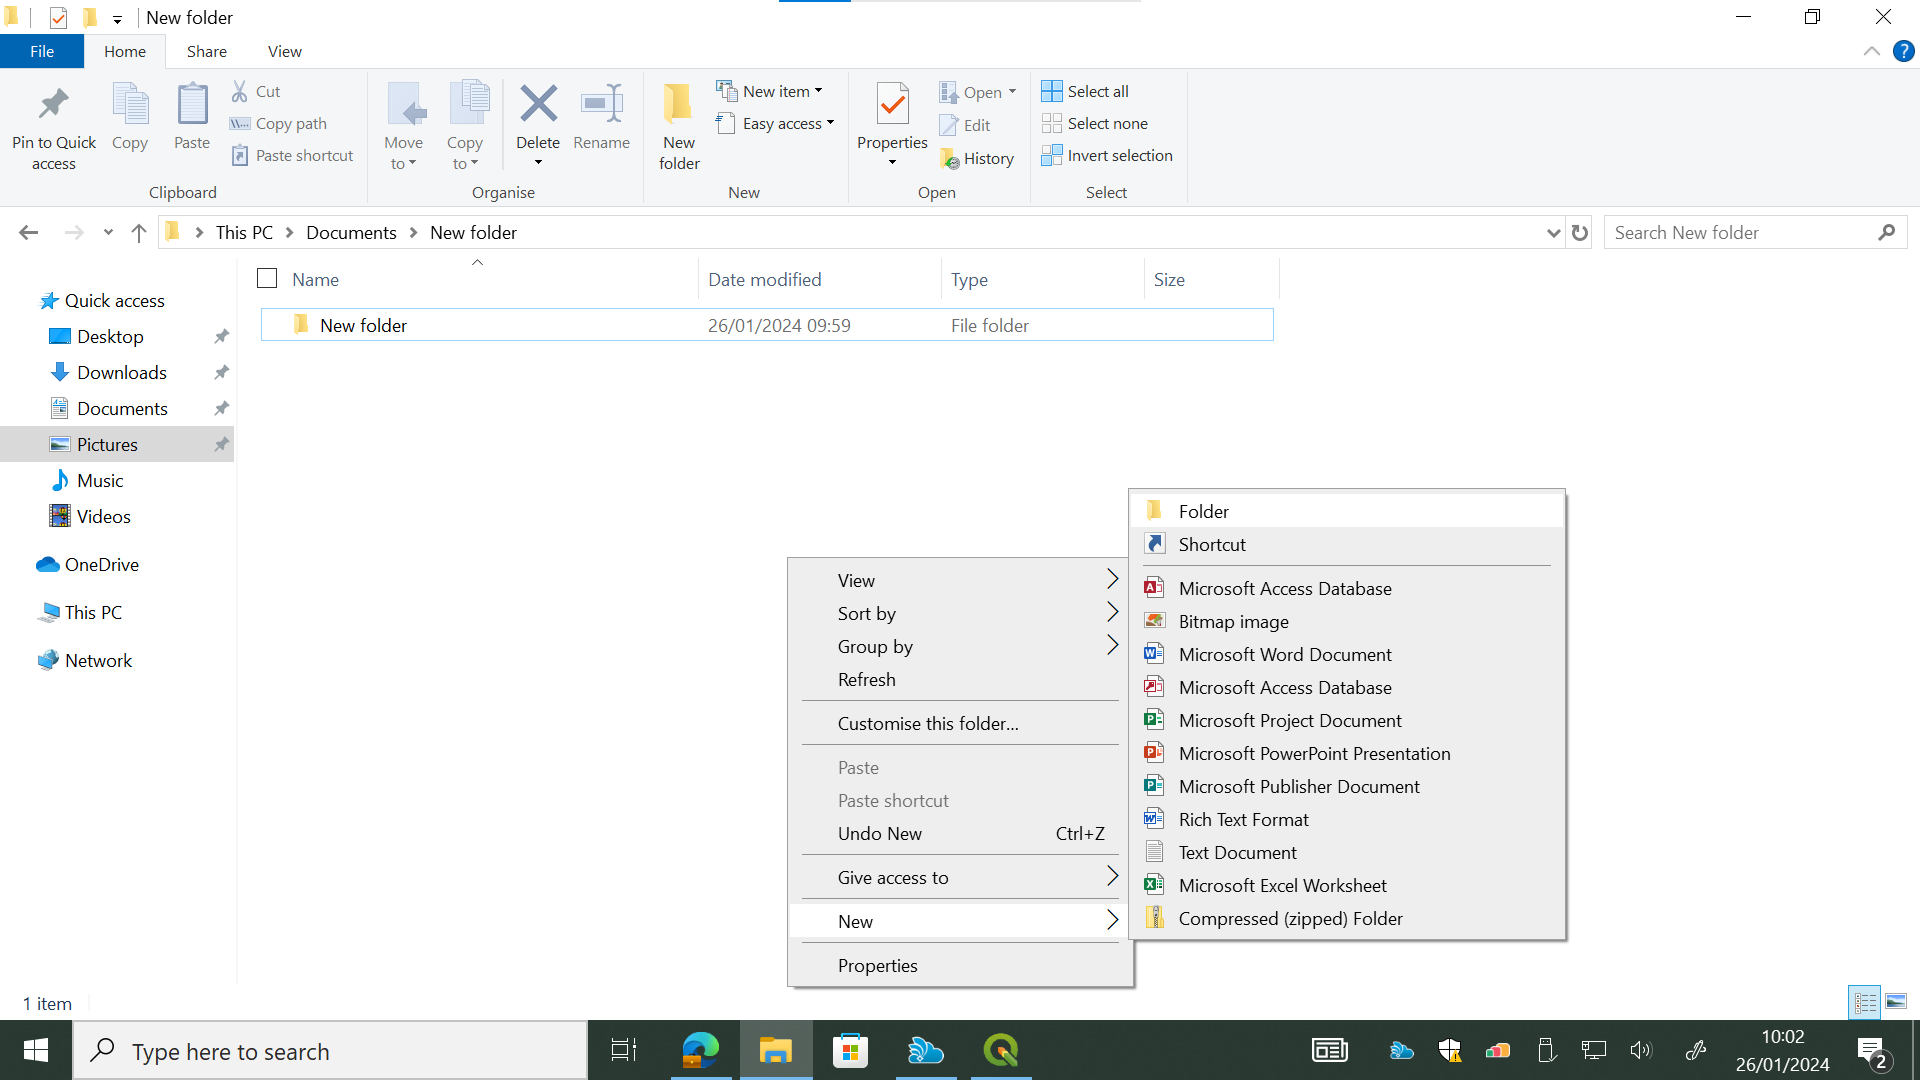
\includegraphics{images/lab_1/lab1_fig3_wincfolder.png}

\textbf{mac OS:}

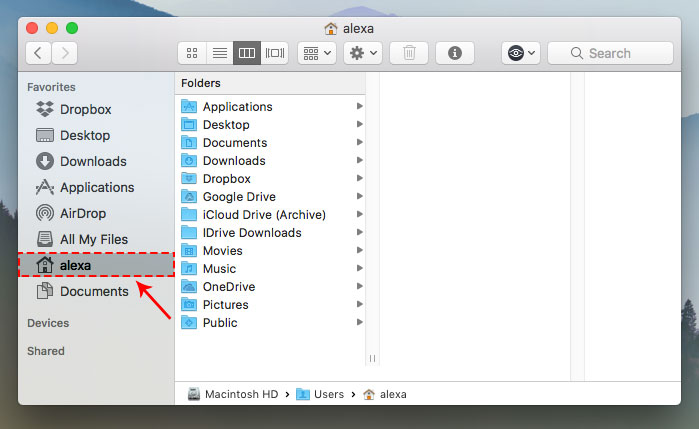
\includegraphics{images/lab_1/lab1_fig3_macfolder.png}

\begin{tcolorbox}[enhanced jigsaw, coltitle=black, toprule=.15mm, breakable, opacitybacktitle=0.6, left=2mm, colback=white, leftrule=.75mm, rightrule=.15mm, colbacktitle=quarto-callout-warning-color!10!white, toptitle=1mm, titlerule=0mm, colframe=quarto-callout-warning-color-frame, arc=.35mm, bottomtitle=1mm, opacityback=0, bottomrule=.15mm, title=\textcolor{quarto-callout-warning-color}{\faExclamationTriangle}\hspace{0.5em}{Warning}]

\begin{itemize}
\item
  Having complex file paths can sometimes create problems. That is why
  we try to keep our main projects on a base folder. If you would like
  to keep a copy of your data on your OneDrive folder you are encouraged
  to do so, but I don't recommend working directly from it. That is
  because the full path to a OneDrive folder will to be very long and
  likely contain spaces. Mine, for example is
  \texttt{C:\textbackslash{}Users\textbackslash{}Thiago\textbackslash{}OneDrive\ -\ University\ of\ Stirling\textbackslash{}Documents}.
  Those spaces in the name may create problems later. So I recommend
  instead to \emph{copy} the completed lab data to your OneDrive folder
  at the end of each lab.
\item
  For the same reason, \textbf{never} use spaces or special symbols on
  your folder and file names. Limit yourself to using letters A-Z and
  a-z, numbers 1-9 and just the \emph{underline} (\_) and \emph{dash}
  (-) symbols.
\item
  Windows \textbf{does not} differentiate letter case, so if you create
  a file named \texttt{filename1.txt} and then a second file named
  \texttt{Filename1.txt} in the same folder, the second will overwrite
  the first. Mac OS does differentiate upper and lower case letters, so
  \texttt{Filename1.txt} and \texttt{filename1.txt} are considered
  different names and can co-exist in the same folder.
\end{itemize}

\end{tcolorbox}

\begin{enumerate}
\def\labelenumi{(\arabic{enumi})}
\setcounter{enumi}{4}
\item
  Inside the new \texttt{GEOU9SP} folder, create a subfolder called
  \texttt{lab\_1} (notice I am avoiding spaces by using the underline)
\item
  Inside \texttt{lab\_1}, create the following folder structure. On the
  diagram below, the folder \texttt{raster} is a folder inside the
  folder \texttt{01\_raw\_data}, which is inside \texttt{lab\_1} and so
  on.
\end{enumerate}

\begin{verbatim}
.
└── GEOU9SP/
    └── lab_1/
        ├── 00_qgis
        ├── 01_raw_data/
        │   ├── raster
        │   └── vector
        ├── 02_processing
        ├── 03_final_products
        └── 04_notes
\end{verbatim}

I like to start folder names start with double digits so they are kept
in order. These folders will be used as follows:

\begin{itemize}
\item
  \texttt{00\_qgis}: we will use this folder to save our QGIS project
  files.
\item
  \texttt{01\_raw\_data}: this folder will keep all the original data
  files you download. This way you can always go back to the start if
  something goes wrong. You can optionally use the sub-folders
  \texttt{vector} and \texttt{raster} to easily know which kind of data
  you are working with, but this may not be necessary for small
  projects. As you obtain data you will create additional sub-folders
  for each individual dataset to keep data organized.
\item
  \texttt{02\_processing}: here we will keep all the intermediate files
  you generate as part of your work. Make ample use of sub-folders to
  identify each step of the workflow.
\item
  \texttt{03\_final\_products}: here we will keep the final products of
  our intended analysis. This makes it easy for us to find the latest
  version of our final results, without risking confusing it with
  intermediate files. This can also include maps, reports and any other
  `deliverable' resulting from your analysis.
\item
  \texttt{04\_notes}: here we will keep all our \emph{non-GIS} files.
  For example, it may be a good idea to keep a text file documenting the
  project steps as you work on it. You could also save here screen grabs
  of specific steps. Again, use sub-folders as needed to keep your data
  tidy.
\end{itemize}

\begin{enumerate}
\def\labelenumi{(\arabic{enumi})}
\setcounter{enumi}{6}
\tightlist
\item
  Now move the data you've downloaded into your organized project
  folders and extract (unzip) them if necessary. The terrain data folder
  (\texttt{terrain-50-dtm\_xxxxxxx}) should go into the \texttt{raster}
  folder within \texttt{01\_raw\_data} and the roads folder
  (\texttt{open-roads\_xxxxxxx}) into the \texttt{vector} folder. The
  \texttt{citations\_orders.xxxx.txt} and \texttt{contents\_order\_xxx}
  text files should go into your \texttt{04\_notes} folder. Your folder
  structure should look like this:
\end{enumerate}

\begin{verbatim}
.
└── GEOU9SP/
    └── lab_1/
        ├── 00_qgis
        ├── 01_raw_data/
        │   ├── raster/
        │   │   └── OS_terrain_50/
        │   │       └── ...
        │   └── vector/
        │       └── OS_roads/
        │           └── ...
        ├── 02_processing
        ├── 03_final_products
        └── 04_notes
\end{verbatim}

\begin{tcolorbox}[enhanced jigsaw, coltitle=black, toprule=.15mm, breakable, opacitybacktitle=0.6, left=2mm, colback=white, leftrule=.75mm, rightrule=.15mm, colbacktitle=quarto-callout-important-color!10!white, toptitle=1mm, titlerule=0mm, colframe=quarto-callout-important-color-frame, arc=.35mm, bottomtitle=1mm, opacityback=0, bottomrule=.15mm, title=\textcolor{quarto-callout-important-color}{\faExclamation}\hspace{0.5em}{Stop and Think}]

What are the \texttt{citations\_orders.xxxx.txt} and
\texttt{contents\_order\_xxx} files? What information do they contain?

\end{tcolorbox}

\begin{tcolorbox}[enhanced jigsaw, toprule=.15mm, breakable, left=2mm, colframe=quarto-callout-important-color-frame, colback=white, arc=.35mm, leftrule=.75mm, opacityback=0, rightrule=.15mm, bottomrule=.15mm]

\vspace{-3mm}\textbf{Click for answer}\vspace{3mm}

They are both plain text files. \texttt{citations\_orders.xxxx.txt} is
very handy as it gives us the proper way to cite the data sources on
reports. \texttt{contents\_order\_xxx} is just a summary of your Digimap
order.

\end{tcolorbox}

\begin{enumerate}
\def\labelenumi{(\arabic{enumi})}
\setcounter{enumi}{7}
\tightlist
\item
  Start a new text file (a Word \emph{.doc} file or a Notepad
  \emph{.txt} file) in your \texttt{04\_notes} folder, and write a few
  lines documenting the steps you took until now. If you prefer
  handwritten notes on a paper notebook, feel free to use it instead!
  The important thing is to keep track of the steps you are taking. As
  projects get more complicated, it is easy to forget which steps we
  took, and in what order!
\end{enumerate}

\subsection{Creating a QGIS project and adding data to
it}\label{creating-a-qgis-project-and-adding-data-to-it}

A QGIS project is a file, which will remember all the data layers you
have loaded, their stacking order, the styling of each layer, and some
other information such as the coordinate reference system. It will also
keep any map layouts that you create. \textbf{But he project file will
NOT store the data files themselves!!}. It will only link to the data.
That is why we need good project folder organisation. If a data file is
moved or renamed, the QGIS project file will lose track of it.

\begin{enumerate}
\def\labelenumi{\arabic{enumi}.}
\setcounter{enumi}{5}
\tightlist
\item
  Create a new project in QGIS by clicking on
  \texttt{Project\ \textgreater{}\ New...} or pressing \emph{Ctrl-N}:
\end{enumerate}

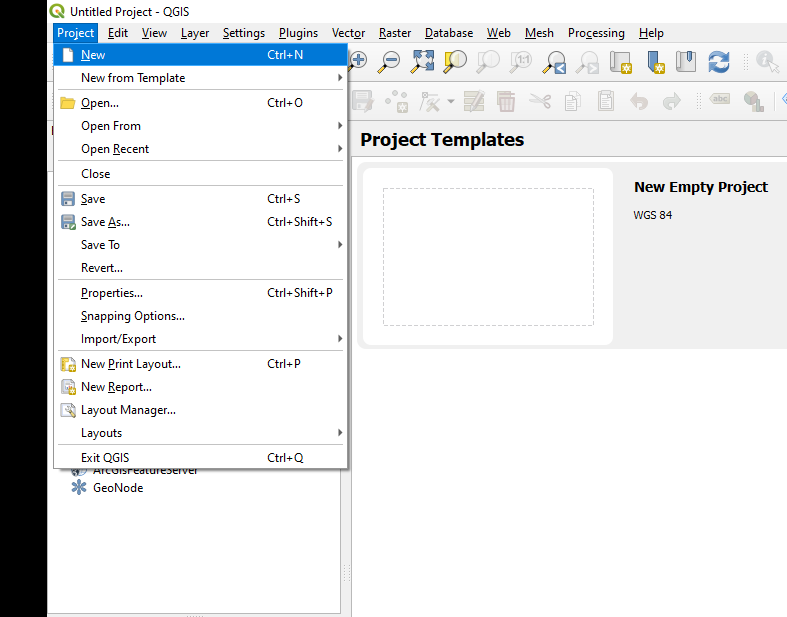
\includegraphics{images/lab_1/lab1_fig1_newproject.png}

\begin{enumerate}
\def\labelenumi{(\arabic{enumi})}
\setcounter{enumi}{8}
\item
  Add to your project the layers \texttt{NS\_RoadLink.shp} from the OS
  Roads dataset and the \texttt{NS89.asc} terrain data from your
  organized project folders. Don't worry if the extents don't match -
  it's just that the OS DEM and the OS Roads are distributed in
  different sized `chunks'.
\item
  Save your project inside the \texttt{00\_qgis} folder. You can save
  your project by clicking on the \emph{Save} button, going to
  \texttt{Project\ \textgreater{}\ Save} menu, or by holding the keys
  \texttt{Ctrl+S\ (Command+S\ on\ Mac)}.
\item
  Open the project settings by clicking on the menu
  \texttt{Project\ \textgreater{}\ Properties...}. You will then see
  this window:
\end{enumerate}

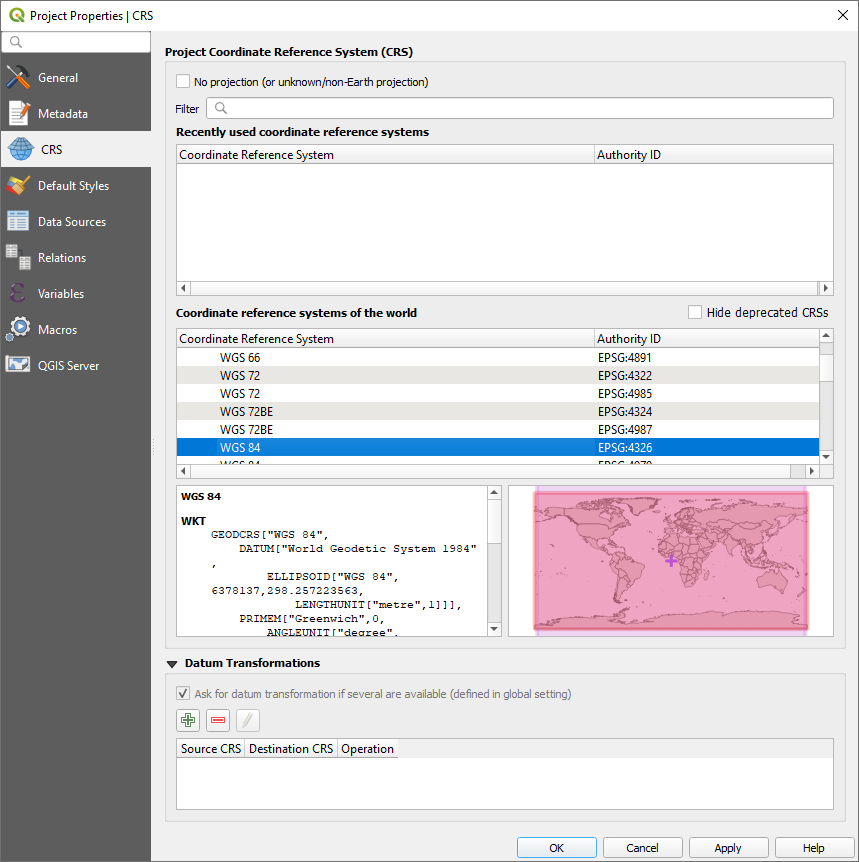
\includegraphics{images/lab_1/lab1_fig2_projprops.png}

\begin{enumerate}
\def\labelenumi{(\arabic{enumi})}
\setcounter{enumi}{11}
\item
  The main things to set on your new project are the project home
  folder, the coordinate reference system (CRS) and the measurement
  units.

  \begin{itemize}
  \item
    As the \emph{project home} on the \texttt{General} tab, select the
    \texttt{lab\_1} folder you created. This helps quick navigation when
    opening and saving data.
  \item
    For \emph{measurement units}, make sure distance units are set in
    meters, and area units in squared meters, also on the
    \texttt{General} tab. Any QGIS operations that calculate distances
    or areas will use the units set by the project.
  \end{itemize}
\end{enumerate}

\begin{itemize}
\tightlist
\item
  For the CRS, go to the \texttt{CRS} tab (to the left) and search for
  \textbf{27700} in the \texttt{Filter} box. That is the \emph{EPSG
  code} that identifies the \emph{OSGB 1936 British National Grid}
  coordinate reference system (CRS). Select it by clicking on it - you
  may need to expand your search results by clicking on the small arrows
  besides \texttt{Projected} and \texttt{Transverse\ Mercator}.
\end{itemize}

\begin{tcolorbox}[enhanced jigsaw, coltitle=black, toprule=.15mm, breakable, opacitybacktitle=0.6, left=2mm, colback=white, leftrule=.75mm, rightrule=.15mm, colbacktitle=quarto-callout-note-color!10!white, toptitle=1mm, titlerule=0mm, colframe=quarto-callout-note-color-frame, arc=.35mm, bottomtitle=1mm, opacityback=0, bottomrule=.15mm, title=\textcolor{quarto-callout-note-color}{\faInfo}\hspace{0.5em}{Note}]

EPSG stands for ``European Petroleum Survey Group'', and designates a
database with standard codes for hundreds of coordinate reference
systems. Over time, you will probably memorize the EPSG codes for the
CRSs you use more often.

\end{tcolorbox}

\begin{enumerate}
\def\labelenumi{(\arabic{enumi})}
\setcounter{enumi}{12}
\tightlist
\item
  Save your project again.
\end{enumerate}

\section{Guided Exercise 2 - Organizing and styling your
layers}\label{guided-exercise-2---organizing-and-styling-your-layers}

One of the most powerful aspects of GIS software is the ability to
\emph{style} spatial data in very specific ways, by specifying colours,
line widths, line types, symbols, etc. As we progress in the module you
will learn more and more ways to style your data.

\begin{enumerate}
\def\labelenumi{(\arabic{enumi})}
\setcounter{enumi}{13}
\item
  On the \texttt{Layers\ panel} to the left of the screen, select the
  \texttt{NS89} layer, and drag it to the bottom of the layers list if
  not there already.
\item
  Turn the roads layer off for now, by unchecking the box besides its
  name.
\item
  Right-click on the \texttt{NS89} layer name and choose
  \texttt{Rename\ Layer}. Rename it to
  \texttt{Digital\ Elevation\ Model\ (50m)}.
\item
  Open the file explorer in your system, and find the \texttt{NS89.asc}
  file that holds the actual elevation data, which you downloaded from
  Digimap.
\end{enumerate}

\begin{tcolorbox}[enhanced jigsaw, coltitle=black, toprule=.15mm, breakable, opacitybacktitle=0.6, left=2mm, colback=white, leftrule=.75mm, rightrule=.15mm, colbacktitle=quarto-callout-important-color!10!white, toptitle=1mm, titlerule=0mm, colframe=quarto-callout-important-color-frame, arc=.35mm, bottomtitle=1mm, opacityback=0, bottomrule=.15mm, title=\textcolor{quarto-callout-important-color}{\faExclamation}\hspace{0.5em}{Stop and Think}]

Will changing a layer name in the layer panel also change the name of
the source data file for that layer?

\end{tcolorbox}

\begin{tcolorbox}[enhanced jigsaw, toprule=.15mm, breakable, left=2mm, colframe=quarto-callout-important-color-frame, colback=white, arc=.35mm, leftrule=.75mm, opacityback=0, rightrule=.15mm, bottomrule=.15mm]

\vspace{-3mm}\textbf{Click for answer}\vspace{3mm}

No, layer names within the project are independent of file names - but
as default QGIS will use the file name as layer name when you add new
data. But you should always change them into nice, readable and properly
spelled names within your project, where you are free to use spaces. The
actual file name linked by the project will stay the same and can always
be seen by right-clicking on the layer name and selecting
\texttt{Properties...\textgreater{}\ Information}.

\end{tcolorbox}

\begin{enumerate}
\def\labelenumi{(\arabic{enumi})}
\setcounter{enumi}{17}
\item
  Right click on the newly renamed terrain layer and choose
  \texttt{Zoom\ to\ Layer}. This is a very handy tool to ``find
  yourself'' if you end up zooming or panning the map too far.
\item
  Right click on the terrain layer name again and select
  \texttt{Properties...}, then go to the \texttt{Symbology} tab.
\item
  On the \texttt{Min} and \texttt{Max} boxes, type \texttt{0} and
  \texttt{500} respectively. This determines the range of layer values
  to be visualised.
\item
  Select \texttt{Rendering\ type} to be
  \texttt{Single\ Band\ Pseudocolor}, and change the
  \texttt{Color\ ramp} option by clicking on the down-arrow button to
  the right and picking the \texttt{spectral} colour ramp. If you click
  on the colour ramp itself it will open a new window to customise it.
  This is now what we need for now, so just close it and use the
  down-arrow.
\item
  Click on \texttt{Classify} (under the drop down menu that says * Mode:
  continuous*). The colours will be matched to the range of elevation
  values in the layer.
\item
  Click again on the little down-arrow button beside the colour palette
  button and select \texttt{Invert\ Color\ Ramp} at the top of the
  options, so that the lowest heights are coloured blue. Then click on
  \texttt{OK}.
\item
  Note how the legend for you terrain layer has changed on the Layers
  panel. It now shows the minimum and maximum elevations and the colour
  ramp. Save your project.
\end{enumerate}

\begin{tcolorbox}[enhanced jigsaw, coltitle=black, toprule=.15mm, breakable, opacitybacktitle=0.6, left=2mm, colback=white, leftrule=.75mm, rightrule=.15mm, colbacktitle=quarto-callout-important-color!10!white, toptitle=1mm, titlerule=0mm, colframe=quarto-callout-important-color-frame, arc=.35mm, bottomtitle=1mm, opacityback=0, bottomrule=.15mm, title=\textcolor{quarto-callout-important-color}{\faExclamation}\hspace{0.5em}{Stop and Think}]

Why do we bother inverting the colour ramp for this dataset?

\end{tcolorbox}

\begin{tcolorbox}[enhanced jigsaw, toprule=.15mm, breakable, left=2mm, colframe=quarto-callout-important-color-frame, colback=white, arc=.35mm, leftrule=.75mm, opacityback=0, rightrule=.15mm, bottomrule=.15mm]

\vspace{-3mm}\textbf{Click for answer}\vspace{3mm}

We should always try to use colours that reinforce map interpretation.
The colour blue is usually associated with water, and water accumulates
on the lowest elevations, so setting the lowest elevations to blue helps
map users read and interpret the map.

\end{tcolorbox}

\begin{enumerate}
\def\labelenumi{(\arabic{enumi})}
\setcounter{enumi}{24}
\item
  Rename the \texttt{NS\_RoadLink} layer to \texttt{Road\ Network}.
\item
  Go to its \texttt{Symbology} properties, like you did for the terrain
  layer, Notice that the symbology options are data-specific (vector
  vs.~raster). Select \texttt{Simple\ Line} in the symbology window
  (under the main \texttt{Line} option). Then under the window, go to
  the \texttt{Color} option an click on the down-arrow menu to change
  the line colour to a dark grey. If you click on the actual colour, a
  more complex colour-picking window will appear. You can use either the
  quicker colour drop down or the main colour window, whatever you
  prefer.
\item
  Change the \texttt{Stroke\ width} (line width) to 0.3. Click
  \texttt{OK}. Reactivate the layer if needed to visualise it.
\end{enumerate}

\section{Guided Exercise 3: Processing data using GIS
operations}\label{guided-exercise-3-processing-data-using-gis-operations}

The core of GIS work is to use the many built-in operations (also known
as functions or tools) of GIS software to \emph{process} the data in
some way, and thus create additional information. For this exercise, we
will use an operation that creates a new layer representing the
boundaries of the terrain data layer, and then use a second operation to
cut the roads layer to the same shape and extent as this new layer.

\begin{enumerate}
\def\labelenumi{(\arabic{enumi})}
\setcounter{enumi}{27}
\item
  Go to the \texttt{Vector} menu and select
  \texttt{Research\ Tools\ \textgreater{}\ Extract\ Layer\ Extent...}.
  Select the terrain layer as your \texttt{Input\ layer}, and click
  \texttt{Run} to generate a \emph{temporary layer}. Temporary layers
  are not kept once you close QGIS, unless you save it manually later.
  The \texttt{Extract\ Layer\ Extent} window will not close
  automatically after you run the operation, so click on \texttt{Close}
  when you are done.
\item
  Go to
  \texttt{Vector\ \textgreater{}\ Geoprocessing\ Tools\ \textgreater{}\ Clip...}.
  Select the roads layer as the \texttt{Input\ Layer} and the new
  temporary layer as the \texttt{Overlay\ Layer}.
\item
  This time, we will save the output. Click on the \texttt{...} button
  to the right of the \texttt{Clipped} text box, and then choose
  \texttt{Save\ to\ file}. Save your new layer on the folder
  \texttt{GEOU9SP/lab\_1/02\_processing/}, naming it
  \texttt{clipped\_roads.shp}. Make sure the \texttt{SHP\ file} format
  is selected below the file name. Then click on \texttt{Run} to execute
  the operation. Close the window.
\item
  Turn the original roads layer on and off to see the result of your
  operation. Then right-click on the original roads layer, and select
  \texttt{Styles\ \textgreater{}\ Copy\ Style\ \textgreater{}\ All\ Style\ Categories}.
  Then right click on the new (\texttt{Clipped}) roads layer and select
  \texttt{Styles\ \textgreater{}\ Paste\ Style\ \textgreater{}\ All\ Style\ Categories}.
  This is a great way to style several layers in the same way without
  effort.
\item
  Remove the original roads layer from your project by right clicking on
  it and selecting \texttt{Remove\ Layer...}, and then rename you
  clipped layer to ``Roads''. Save your project.
\item
  Close QGIS. \textbf{It will give you a warning} - read it carefully
  and then confirm it.
\item
  Reopen QGIS, and load your project again. Notice it remembers exactly
  where you last saved it, including zoom level, layer names and layer
  styles. The ``Extent'' layer will still be on your list but will
  appear empty - it has been deleted once you closed QGIS. Remove it
  from the project and save again.
\end{enumerate}

\begin{tcolorbox}[enhanced jigsaw, coltitle=black, toprule=.15mm, breakable, opacitybacktitle=0.6, left=2mm, colback=white, leftrule=.75mm, rightrule=.15mm, colbacktitle=quarto-callout-important-color!10!white, toptitle=1mm, titlerule=0mm, colframe=quarto-callout-important-color-frame, arc=.35mm, bottomtitle=1mm, opacityback=0, bottomrule=.15mm, title=\textcolor{quarto-callout-important-color}{\faExclamation}\hspace{0.5em}{Stop and Think}]

\begin{enumerate}
\def\labelenumi{\alph{enumi})}
\item
  What are the names of the two GIS functions you just used in this
  exercise?
\item
  Why did you have to create a new layer representing the extent of the
  terrain data before \emph{clipping} the roads layer?
\item
  What does the warning given by QGIS when you closed your project mean?
\end{enumerate}

\end{tcolorbox}

\begin{tcolorbox}[enhanced jigsaw, toprule=.15mm, breakable, left=2mm, colframe=quarto-callout-important-color-frame, colback=white, arc=.35mm, leftrule=.75mm, opacityback=0, rightrule=.15mm, bottomrule=.15mm]

\vspace{-3mm}\textbf{Click for answer}\vspace{3mm}

\begin{enumerate}
\def\labelenumi{\alph{enumi})}
\item
  The functions are called \texttt{Clip} and
  \texttt{Extract\ Layer\ Extent}.
\item
  The \texttt{Clip} function requires two \emph{vector} files as input,
  but the terrain data is a \emph{raster} file (i.e.~an image). The
  \texttt{Extract\ Layer\ Extent} creates a vector file representing the
  extent of any given layer. Each specific tool will require different
  kinds of data to work properly. We will learn more about vectors and
  rasters in weeks 2 and 3.
\item
  When we created the extent layer, we produced a \emph{temporary
  layer}, which is discarded by QGIS when the program is closed. QGIS
  was letting you know that will happen, to give you the chance to go
  back and save it. Temporary layers are also lost when QGIS crashes
  (yes when, not if - it will happen). So never use them for important
  stuff - only for quick tests if you are not sure what the output of a
  function will be.\\
\end{enumerate}

\end{tcolorbox}

\section{Guided Exercise 4: Creating a map
layout}\label{guided-exercise-4-creating-a-map-layout}

The main QGIS interface (or any other GIS software) is developed and
optimised for interactive work. But very often as part of our GIS
analysis we will want to generate nice maps and figures following proper
design rules (and not just grabbing a screen capture of the QGIS window
and dumping it on a page - hint for your assignment reports). For that,
we use the QGIS \textbf{Map Layout Editor}.

\begin{enumerate}
\def\labelenumi{(\arabic{enumi})}
\setcounter{enumi}{34}
\item
  Click on \texttt{Project\ \textgreater{}\ New\ Print\ Layout} and name
  it \texttt{Lab\ 1\ Layout}. A new window will open showing the QGIS
  Layout Editor. Notice that the main QGIS window remains open as well.
  These windows are `linked', so that the map layout reflects any
  styling changes you make on the main window.
\item
  Add a new map to the layout by clicking on the
  
\includegraphics{index_files/mediabag/mActionAddMap.png} icon. Drag it
  through the page so it covers about 2/3 of it horizontally, and the
  full height of the page (minus some borders).
\item
  Use the \texttt{Interactive\ Extent} tool
  
\includegraphics{index_files/mediabag/mActionMoveItemConte.png} to pan
  (click and drag) and zoom (mouse wheel) until your data covers the
  entire map box. But make sure you don't hide the edges of the data by
  zooming in too much!
\item
  Now fine tune the map scale by changing the \texttt{Scale} value on
  the bottom right panel. Remember that this value means ``1:value'',
  i.e.~one unit on the page is equal to that many units (value) in the
  real world. This means larger numbers will ``zoom out'', and smaller
  numbers will ``zoom in''. Try to make the map fill as much as possible
  of the map box, without clipping the edges.
\item
  Go to the menu \texttt{Add\ Item\ \textgreater{}\ Add\ Legend...} in
  the Map Layout Window (or guess the icon for this option on the side
  toolbar). Click the area beside the map box and drag to add a legend.
\item
  Go back to the main QGIS window, right click on the terrain layer
  name, then select \texttt{Properties...}, and on the
  \texttt{Symbology} tab, change the \texttt{Mode} under the class
  colour box to \texttt{Equal\ Interval}. Then select the number of
  \texttt{Classes} to 10 (to the right of the \texttt{Equal\ Interval}
  box). Go back to the Map Layout editor.
\item
  Go to the menu \texttt{Add\ Item\ \textgreater{}\ Add\ Scalebar} in
  the Map Layout Window (or guess the icon for this option on the side
  toolbar). Click and drag in the area below the legend to add it to the
  map layout.
\item
  Add a title to your map using the \texttt{Add\ Label...} tool (either
  on the \texttt{Add\ Item} menu or selecting the tool directly from the
  left sidebar). You can change the text by replacing the ``Lorem
  ipsum'' placeholder text with your own text on the left pane. Try to
  make it \textbf{bold} with a font size of 16 (hint: always use the
  down-arrow buttons for `quick settings').
\item
  Rearrange the items on the page until you are pleased with the
  results. Then go to
  \texttt{Layout\ \textgreater{}\ Export\ as\ PDF...}, and export your
  map, naming it properly and saving it on
  \texttt{GEOU9SP/lab\_1/final\_products}. It is a good idea to export
  as PDF if you want your map to be a standalone document. If you are
  exporting to insert the map into a report, then use
  \texttt{Layout\ \textgreater{}\ Export\ as\ Image...} instead.
\end{enumerate}

For reference, my map looked like this at this stage:

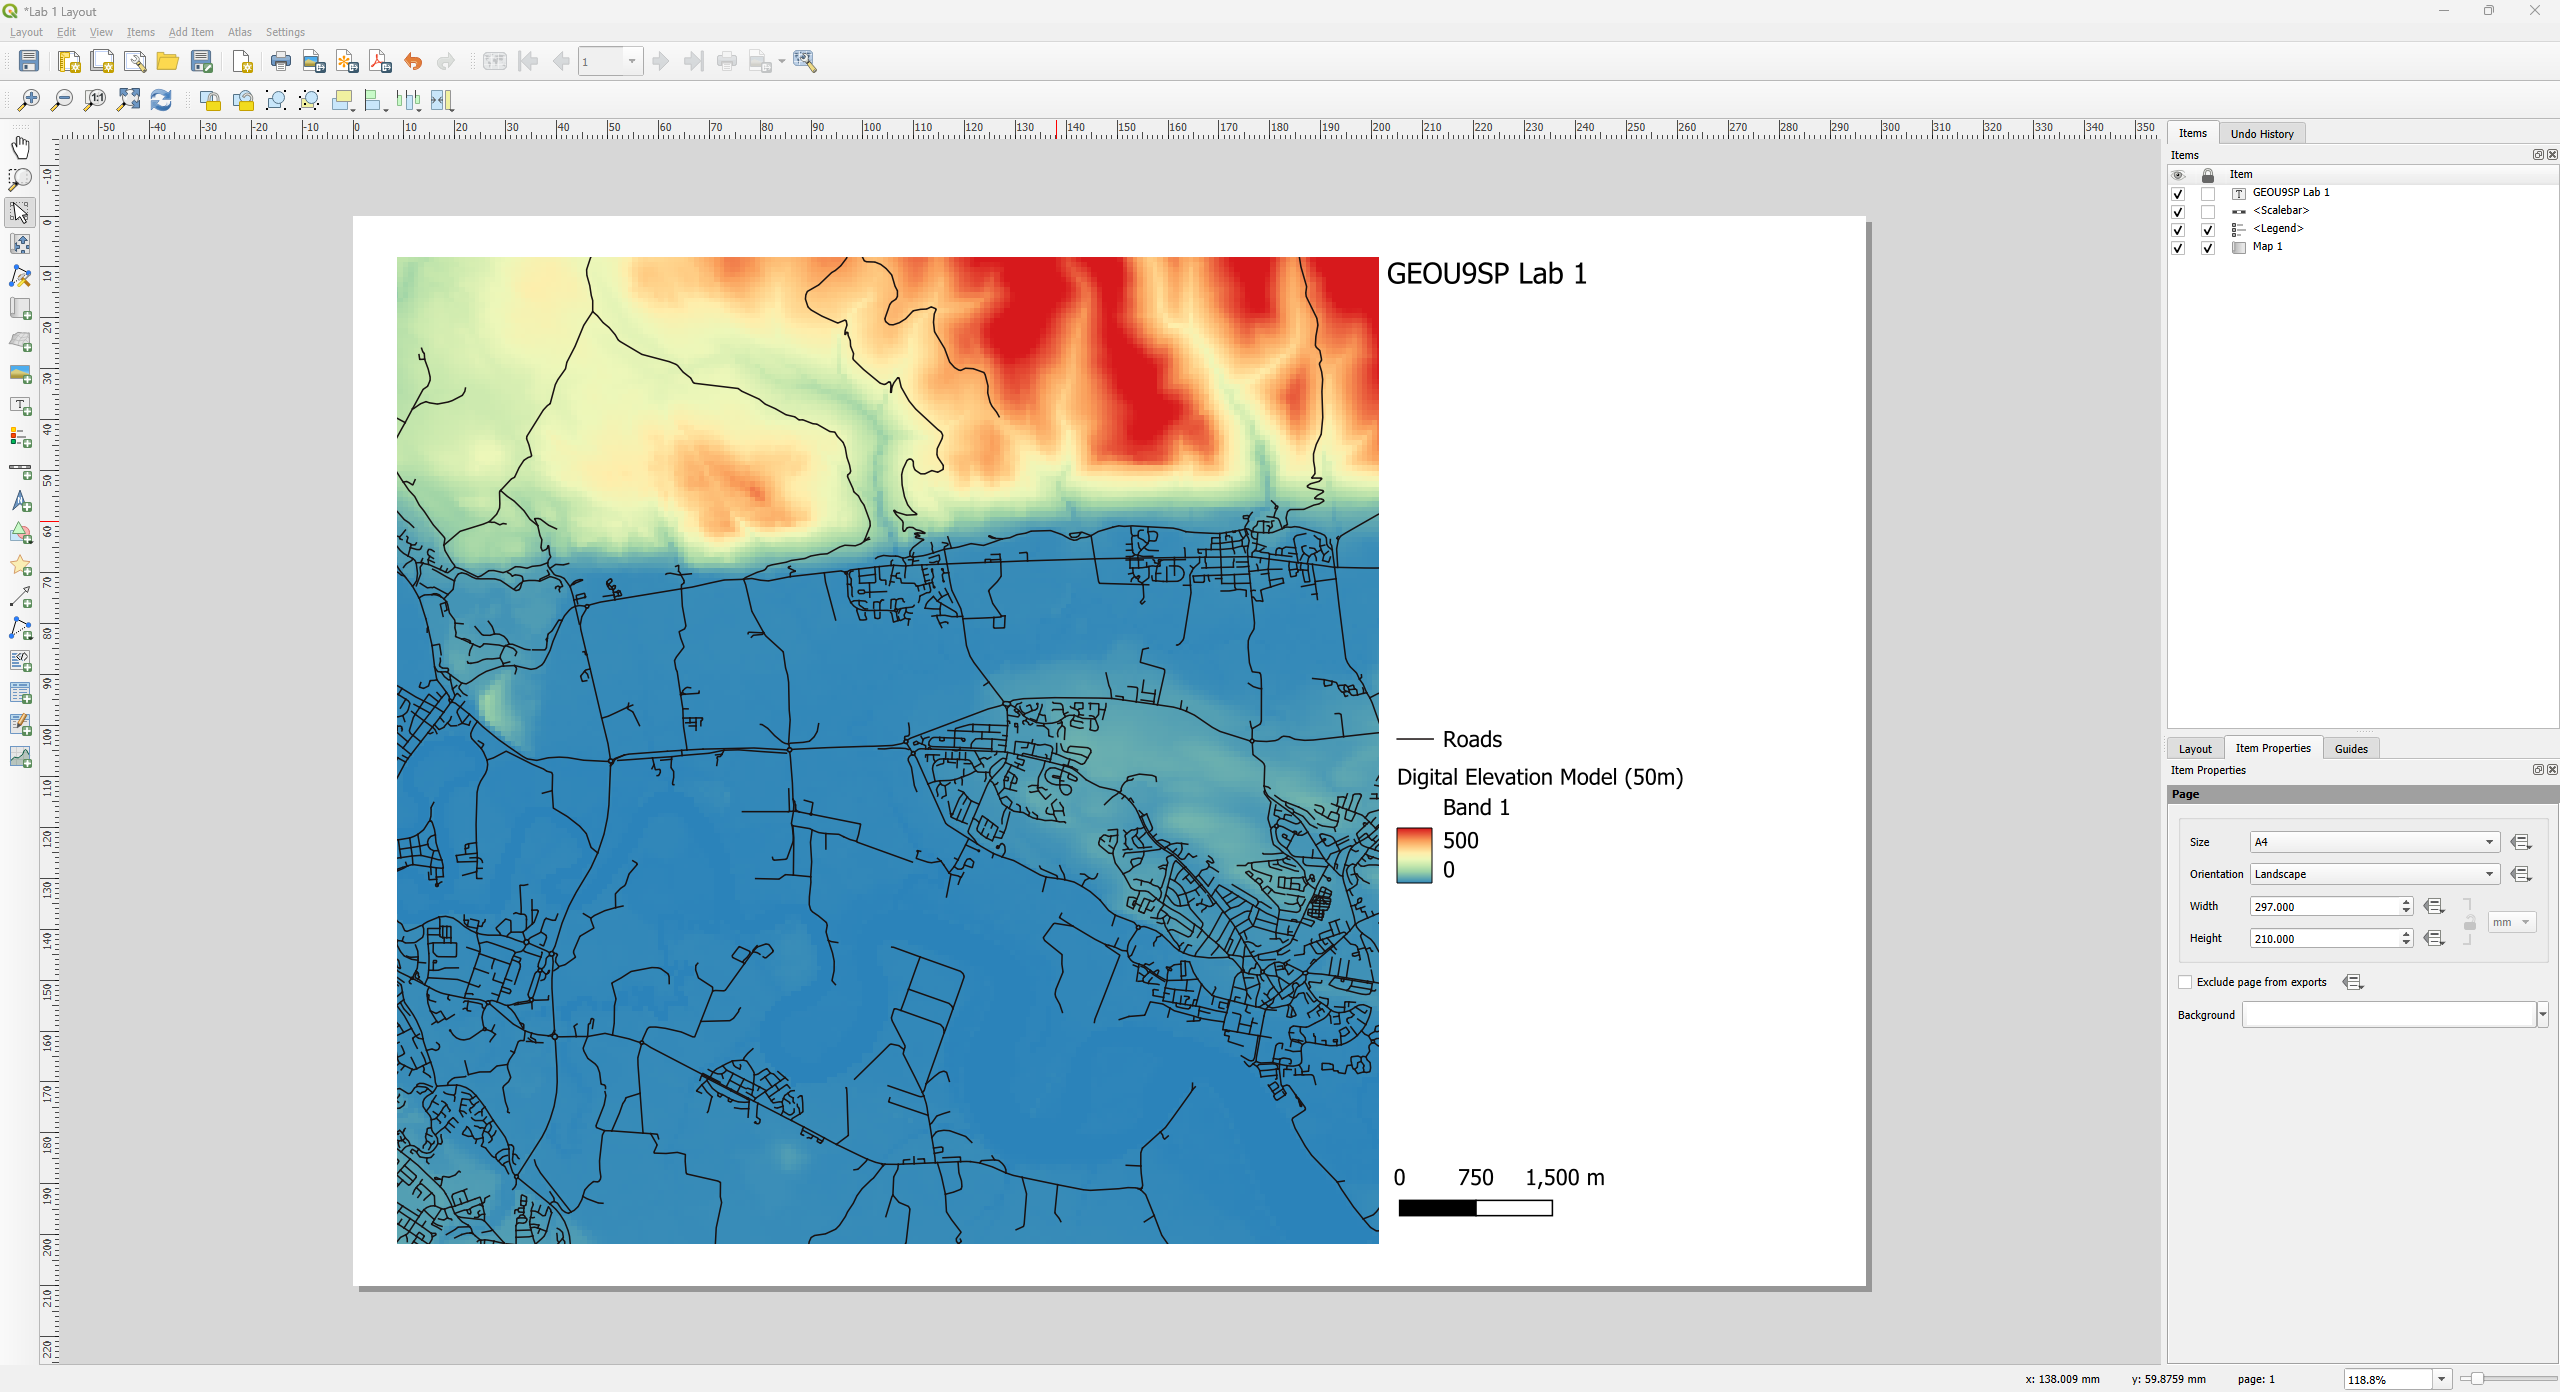
\includegraphics{images/lab_1/lab1_fig6_mapzoom.png}

\begin{enumerate}
\def\labelenumi{(\arabic{enumi})}
\setcounter{enumi}{43}
\tightlist
\item
  Then close the Map Layout window, save your project on the main QGIS
  window, and close QGIS. Reopen QGIS, and go to
  \texttt{Project\ \textgreater{}\ Layout\ Manager}. The layout you
  created previously should appear on the list. Select it and click on
  \texttt{Show} to reopen the Map Layout window.
\end{enumerate}

\textbf{Congratulations!} You have successfully finished your first GIS
project, using proper file management practices! As a final suggestion,
create a ``workflow\_notes'' file on \texttt{GEOU9SP/lab1/notes} and
write up a quick overview of what you did, along with any specific notes
you would like to remember later.

\section{Independent Exercise 1}\label{independent-exercise-1}

At the end of each lab, you will have the opportunity to reinforce what
you learned by going through `independent' exercises. These will use the
same operations you learned with the guided exercises, but it may
require you to figure out small bits of new functionality and will not
have step by step instructions.

As the module progresses, the independent exercises will give you less
and less directions, to reflect real-world GIS usage. \textbf{Make sure
you do the independent exercises} - it is easy to fall into a false
sense of `\emph{I got this}' when only following step-by-step
directions.

\begin{enumerate}
\def\labelenumi{\arabic{enumi}.}
\item
  Create a new project folder structure for this project, under your
  main GEOU9SP work folder.
\item
  Download the zipfile containing the Air Photo Mosaic and the Stirling
  Council Geospatial Data from
  \href{https://stir-my.sharepoint.com/:u:/g/personal/ala2_stir_ac_uk/EWxq18uE5uRAjh_fGHf1qC4BRKxp-M4QTs0e1qttSa_m_Q?e=oPnFWQ}{here}.
\item
  Extract the data from the zipfiles and move them to the proper project
  folders.
\item
  Open QGIS and create a new project that uses the OSGB British Grid
  (EPSG 27700) coordinate reference system.
\item
  Import the airphoto raster image and the vector files for Buildings,
  Roads, Railway Track, Electricity Transmission Lines, and Functional
  Sites into your QGIS project.
\item
  Organize your layers so that, from top to bottom, you have
  transmission lines, railways, roads, buildings, functional sites, and
  then the airphoto image.
\item
  Style your layers so that transmission lines are styled as thin dashed
  red lines, railways as thick white lines, roads as thick grey lines,
  buildings as filled yellow polygons and functional sites with a thick
  dark blue outline and no fill colour (hint: check the
  \texttt{Fill\ style} options).
\item
  \texttt{Clip} all your vector layers to the extent of the airphoto
  image.
\item
  Create a map layout covering the entire extent of the airphoto. Add a
  title, legend and scale bar to your layout and export it as a PNG
  image. Then insert your exported file as a figure into a MS Word
  document.
\end{enumerate}

\begin{tcolorbox}[enhanced jigsaw, toprule=.15mm, breakable, left=2mm, colframe=quarto-callout-important-color-frame, colback=white, arc=.35mm, leftrule=.75mm, opacityback=0, rightrule=.15mm, bottomrule=.15mm]

\vspace{-3mm}\textbf{Click here to see what the final layout should look like.}\vspace{3mm}

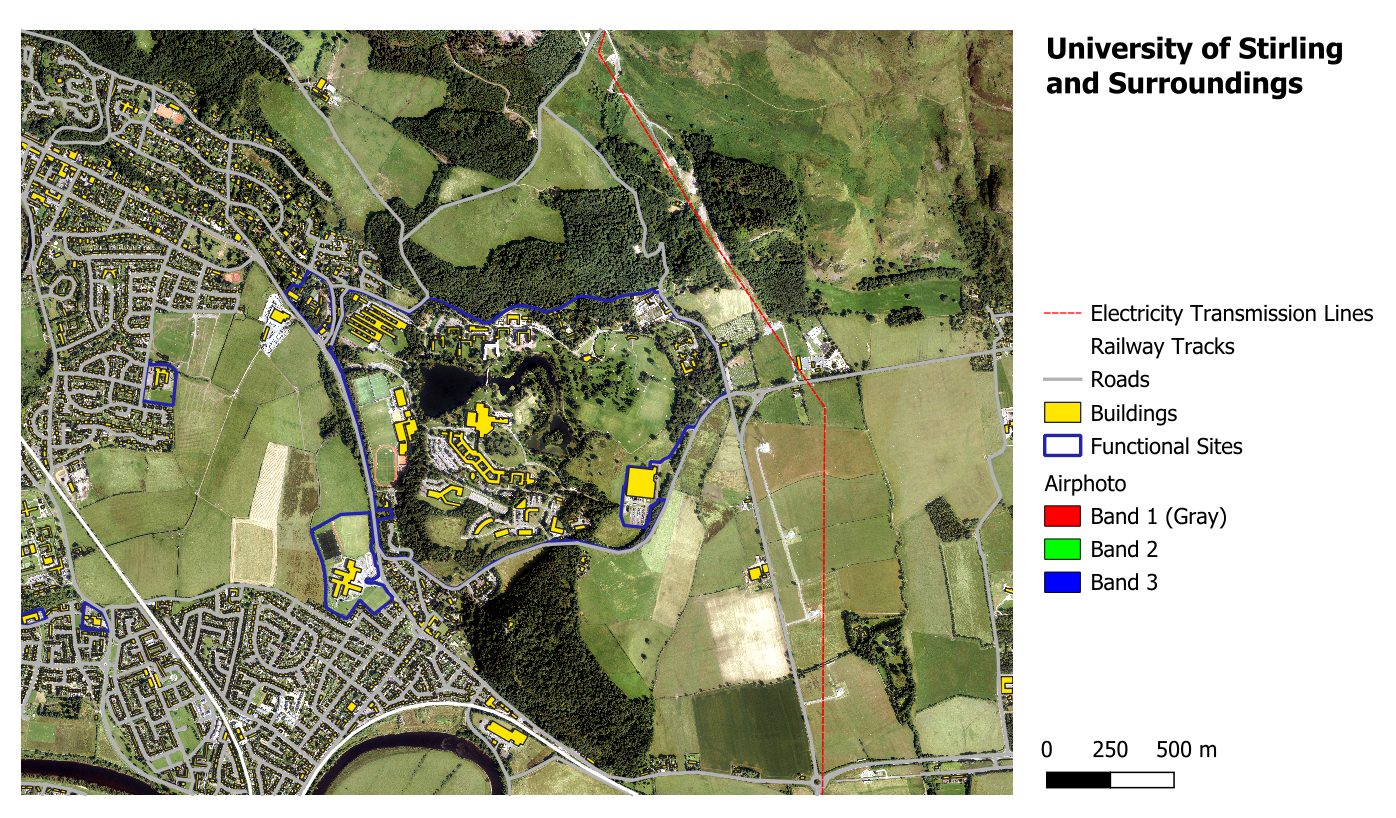
\includegraphics{images/lab_1/lab1_fig7_indmap.png}

\end{tcolorbox}

\begin{enumerate}
\def\labelenumi{\arabic{enumi}.}
\setcounter{enumi}{9}
\tightlist
\item
  Now answer the questions below:
\end{enumerate}

\begin{itemize}
\item
  How far is the Pathfoot Building from the Cottrell Building? Calculate
  it both ``as the crow flies'' (linear distance) and as if you were
  walking. (Hint: use the
  \href{https://docs.qgis.org/3.34/en/docs/user_manual/map_views/map_view.html\#sec-measure}{Measuring}
  tool).
\item
  What is the total surface area of the water bodies in the University
  of Stirling Campus? (Hint: also the Measuring tool).
\item
  What is the classification of the UoS campus polygon within the
  ``Functional Site'' layer? (Hint: use the
  \href{https://docs.qgis.org/3.34/en/docs/user_manual/introduction/general_tools.html\#identify}{Indentify
  Features} tool).
\end{itemize}

\chapter{Lab 2: Coordinate Reference Systems}\label{sec-excrs}

The purpose of this lab is to help you understand why we need to pay
attention to Coordinate Reference Systems (CRS) when working with
spatial data. CRS's are what make data \emph{spatial} - they associate
the actual data to locations on the surface of the Earth (or other
planets!). But there are dozens of CRS's in existence, each adapted for
a specific world region and purpose. So quite often you will obtain
spatial data in different coordinate systems, which can cause problems
if not normalised before analysis.

\section{Guided Exercise 1: Understanding Coordinate Reference
Systems}\label{guided-exercise-1-understanding-coordinate-reference-systems}

In this exercise, you will learn how to use QGIS to identify the
coordinate reference system (CRS, sometimes wrongly called as just
``projection'') of spatial data you acquire and how to manage data and
project coordinate reference systems.

\begin{tcolorbox}[enhanced jigsaw, coltitle=black, toprule=.15mm, breakable, opacitybacktitle=0.6, left=2mm, colback=white, leftrule=.75mm, rightrule=.15mm, colbacktitle=quarto-callout-important-color!10!white, toptitle=1mm, titlerule=0mm, colframe=quarto-callout-important-color-frame, arc=.35mm, bottomtitle=1mm, opacityback=0, bottomrule=.15mm, title=\textcolor{quarto-callout-important-color}{\faExclamation}\hspace{0.5em}{Stop and Think}]

Why are coordinate reference systems and `projections' not the same
thing?

\end{tcolorbox}

\begin{tcolorbox}[enhanced jigsaw, toprule=.15mm, breakable, left=2mm, colframe=quarto-callout-important-color-frame, colback=white, arc=.35mm, leftrule=.75mm, opacityback=0, rightrule=.15mm, bottomrule=.15mm]

\vspace{-3mm}\textbf{Click for answer}\vspace{3mm}

Coordinate reference systems combine a \textbf{datum}, which defines a
geometric representation of the Earth's shape and how it `intersects'
with the real surface of the Earth, a \textbf{coordinate system} (for
example latitude and longitude or northings and eastings) and a
\textbf{map projection} which is a set of mathematical rules to project
the 3D surface of the datum's \emph{ellipsoid} into a flat plane (such
as a screen or a map).

\end{tcolorbox}

\subsection{Obtaining the required
data}\label{obtaining-the-required-data}

\begin{enumerate}
\def\labelenumi{(\arabic{enumi})}
\setcounter{enumi}{44}
\tightlist
\item
  For this exercise, we will use the the \textbf{2024} country
  boundaries data in \textbf{GeoJSON} format, at the \textbf{1:20}
  million scale, that is availabl from the link below. The GeoJSON
  format is a more recent GIS file format, commonly used for web-based
  mapping. It is derived from the JavaScript Object Notation (JSON) data
  file format, widely used to exchange data among websites and web
  servers. More info \href{https://en.wikipedia.org/wiki/GeoJSON}{here}.
\end{enumerate}

\url{https://ec.europa.eu/eurostat/web/gisco/geodata/administrative-units/countries}

We will need two files for this exercise:

\begin{itemize}
\tightlist
\item
  The \emph{boundaries} geometry type (BN) file in the \emph{EPSG:4326}
  coordinate reference system.
\item
  The \emph{boundaries} geometry type (BN) file in the \emph{EPSG:3035}
  coordinate reference system.
\end{itemize}

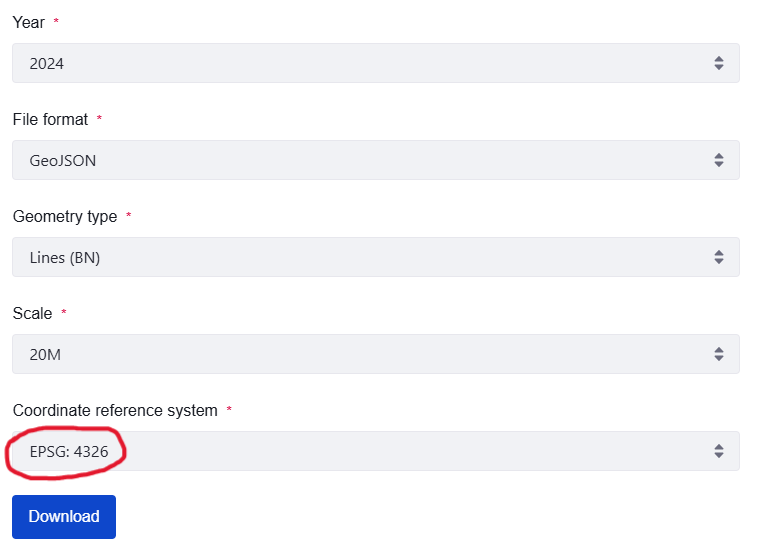
\includegraphics{images/lab_2/lab2_fig1_eurostat_4326.png}

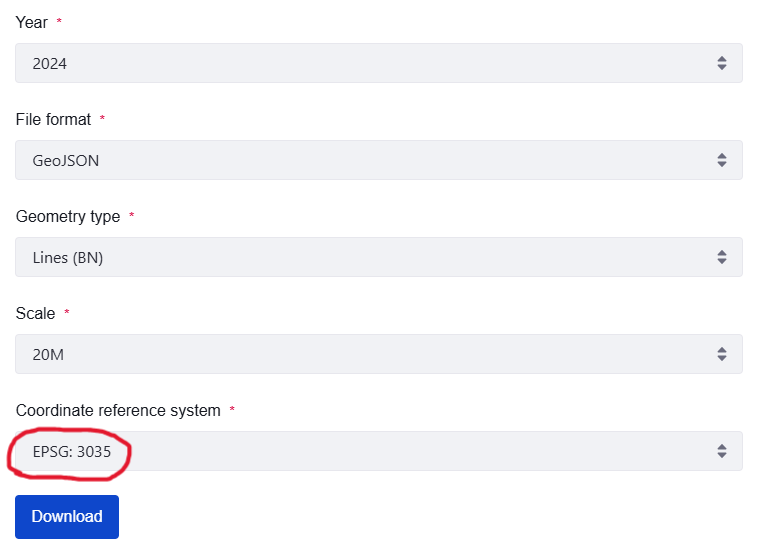
\includegraphics{images/lab_2/lab2_fig1_eurostat_3035.png}

\begin{tcolorbox}[enhanced jigsaw, coltitle=black, toprule=.15mm, breakable, opacitybacktitle=0.6, left=2mm, colback=white, leftrule=.75mm, rightrule=.15mm, colbacktitle=quarto-callout-important-color!10!white, toptitle=1mm, titlerule=0mm, colframe=quarto-callout-important-color-frame, arc=.35mm, bottomtitle=1mm, opacityback=0, bottomrule=.15mm, title=\textcolor{quarto-callout-important-color}{\faExclamation}\hspace{0.5em}{Stop and Think}]

\begin{enumerate}
\def\labelenumi{\alph{enumi})}
\item
  What is the source of the data you are downloading? Does it seem
  reliable?
\item
  What are the conditions (provisions) of use for the data?
\end{enumerate}

\end{tcolorbox}

\begin{tcolorbox}[enhanced jigsaw, toprule=.15mm, breakable, left=2mm, colframe=quarto-callout-important-color-frame, colback=white, arc=.35mm, leftrule=.75mm, opacityback=0, rightrule=.15mm, bottomrule=.15mm]

\vspace{-3mm}\textbf{Click for answer}\vspace{3mm}

\begin{enumerate}
\def\labelenumi{\alph{enumi})}
\item
  The page providing the data is managed by Eurostat, the statistical
  office of the European Union. Therefore, you would be inclined to
  trust in the quality and correctness of the data provided.
\item
  The webpage presents a link to
  ``\href{https://ec.europa.eu/eurostat/web/gisco/geodata/administrative-units}{rules}''
  which describe the authorised uses of the data. This information can
  also be found in the data's \emph{metadata} file.
\end{enumerate}

\end{tcolorbox}

\begin{enumerate}
\def\labelenumi{(\arabic{enumi})}
\setcounter{enumi}{45}
\item
  Create a lab\_2 folder in your GEOU9SP main folder. Then create a
  simple folder structure to organise the data.
\item
  Open QGIS and start a new project. Save it as \texttt{lab\_2} in its
  proper folder. Then look at the contents of the folder holding the
  country data, using the
  \href{https://docs.qgis.org/3.34/en/docs/user_manual/managing_data_source/opening_data.html\#the-browser-panel}{QGIS
  browser panel}. If the panel is not available, you can enable it by
  going to the \texttt{View\ \textgreater{}\ Panels} menu and checking
  the box for \texttt{browser}. You should see the two layers on the
  folder:
\end{enumerate}

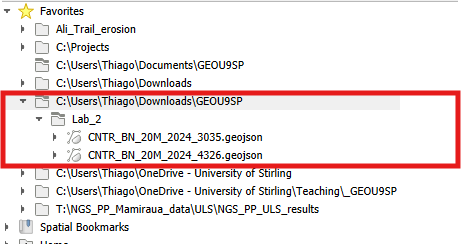
\includegraphics{images/lab_2/lab_2_img2_layers.png}

\begin{enumerate}
\def\labelenumi{(\arabic{enumi})}
\setcounter{enumi}{47}
\tightlist
\item
  Load the \texttt{CNTR\_BN\_20M\_2024\_4326} file into your project.
  Pay attention to the file name as there are many files with similar
  names.
\end{enumerate}

\begin{tcolorbox}[enhanced jigsaw, coltitle=black, toprule=.15mm, breakable, opacitybacktitle=0.6, left=2mm, colback=white, leftrule=.75mm, rightrule=.15mm, colbacktitle=quarto-callout-important-color!10!white, toptitle=1mm, titlerule=0mm, colframe=quarto-callout-important-color-frame, arc=.35mm, bottomtitle=1mm, opacityback=0, bottomrule=.15mm, title=\textcolor{quarto-callout-important-color}{\faExclamation}\hspace{0.5em}{Stop and Think}]

Good file names are always informative of their content. Can you guess
the contents of the different GeoJSON files you have downloaded based on
their names?

\end{tcolorbox}

\begin{tcolorbox}[enhanced jigsaw, toprule=.15mm, breakable, left=2mm, colframe=quarto-callout-important-color-frame, colback=white, arc=.35mm, leftrule=.75mm, opacityback=0, rightrule=.15mm, bottomrule=.15mm]

\vspace{-3mm}\textbf{Click for answer}\vspace{3mm}

All file names start with \texttt{CNTR} for `countries', followed by a
two-letter code. As you seen \texttt{BN} seems to stand for
`boundary'(vector lines), \texttt{RG} for `region'(vector polygons), and
\texttt{LB} for `labels' (vector points). Then \texttt{2024} specified
the reference year, and \texttt{20M} indicates the 1:20 million mapping
scale. The final four-letter number indicates the EPSG code for the data
CRS: 4326 (`unprojected' WGS84), 3857 (WGS 84 with Pseudo-Mercator
projection) or 3035 (ETRS89-extended / Lambert Azimuthal Equal Area for
Europe).

\end{tcolorbox}

\subsection{Visualising data with different
CRS}\label{visualising-data-with-different-crs}

\begin{enumerate}
\def\labelenumi{(\arabic{enumi})}
\setcounter{enumi}{48}
\tightlist
\item
  Set the symbology for the outline and fill as you prefer. Try to
  manipulate more visual variables than just colour.
\end{enumerate}

\begin{tcolorbox}[enhanced jigsaw, coltitle=black, toprule=.15mm, breakable, opacitybacktitle=0.6, left=2mm, colback=white, leftrule=.75mm, rightrule=.15mm, colbacktitle=quarto-callout-important-color!10!white, toptitle=1mm, titlerule=0mm, colframe=quarto-callout-important-color-frame, arc=.35mm, bottomtitle=1mm, opacityback=0, bottomrule=.15mm, title=\textcolor{quarto-callout-important-color}{\faExclamation}\hspace{0.5em}{Stop and Think}]

Why can't you set a fill colour for the countries?

\end{tcolorbox}

\begin{tcolorbox}[enhanced jigsaw, toprule=.15mm, breakable, left=2mm, colframe=quarto-callout-important-color-frame, colback=white, arc=.35mm, leftrule=.75mm, opacityback=0, rightrule=.15mm, bottomrule=.15mm]

\vspace{-3mm}\textbf{Click for answer}\vspace{3mm}

Because the \texttt{BN} files are vector lines, not polygons. Lines only
have one dimension, and thus the inner parts of the countries in this
dataset are actually empty. If you load the \texttt{RG} dataset instead,
you can set the fill, as vector polygons represent 2D areas.

\end{tcolorbox}

\begin{enumerate}
\def\labelenumi{(\arabic{enumi})}
\setcounter{enumi}{49}
\tightlist
\item
  Right-click on this layer's name and go to
  \texttt{Properties\ \textgreater{}\ Information}.
\end{enumerate}

\begin{tcolorbox}[enhanced jigsaw, coltitle=black, toprule=.15mm, breakable, opacitybacktitle=0.6, left=2mm, colback=white, leftrule=.75mm, rightrule=.15mm, colbacktitle=quarto-callout-important-color!10!white, toptitle=1mm, titlerule=0mm, colframe=quarto-callout-important-color-frame, arc=.35mm, bottomtitle=1mm, opacityback=0, bottomrule=.15mm, title=\textcolor{quarto-callout-important-color}{\faExclamation}\hspace{0.5em}{Stop and Think}]

What is the Coordinate Reference System (CRS) for this dataset?

\end{tcolorbox}

\begin{tcolorbox}[enhanced jigsaw, toprule=.15mm, breakable, left=2mm, colframe=quarto-callout-important-color-frame, colback=white, arc=.35mm, leftrule=.75mm, opacityback=0, rightrule=.15mm, bottomrule=.15mm]

\vspace{-3mm}\textbf{Click for answer}\vspace{3mm}

The information tab will have a section called Coordinate Reference
System, as below:

Name: EPSG:4326 - WGS 84 Units: Geographic (uses latitude and longitude
for coordinates) Type: Geographic (2D) Method: Lat/long (Geodetic alias)
Celestial Body: Earth Accuracy: Based on World Geodetic System 1984
ensemble (EPSG:6326), which has a limited accuracy of at best 2 meters.
Reference: Dynamic (relies on a datum which is not plate-fixed)

\end{tcolorbox}

\begin{enumerate}
\def\labelenumi{(\arabic{enumi})}
\setcounter{enumi}{50}
\tightlist
\item
  Note, on the bottom QGIS status bar, that as you move your mouse
  pointer around, the coordinates for the mouse position are updated in
  real time. Also note what the map scale is and how it changes as you
  zoom in and out. You can also type the second part of a scale number
  to zoom at the desired map scale (for example 50000 if you want to see
  the map at a 1:50000 scale)
\end{enumerate}

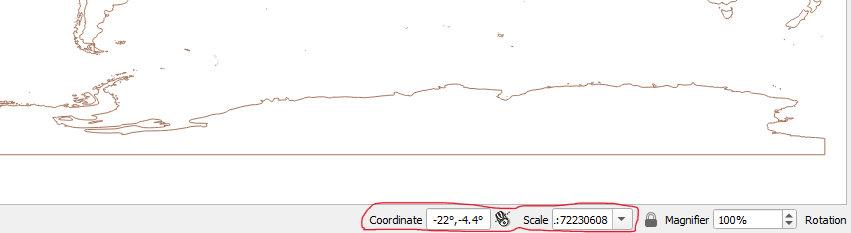
\includegraphics{images/lab_2/lab_2_img4_status_bar.png}

\begin{tcolorbox}[enhanced jigsaw, coltitle=black, toprule=.15mm, breakable, opacitybacktitle=0.6, left=2mm, colback=white, leftrule=.75mm, rightrule=.15mm, colbacktitle=quarto-callout-important-color!10!white, toptitle=1mm, titlerule=0mm, colframe=quarto-callout-important-color-frame, arc=.35mm, bottomtitle=1mm, opacityback=0, bottomrule=.15mm, title=\textcolor{quarto-callout-important-color}{\faExclamation}\hspace{0.5em}{Stop and Think}]

\begin{enumerate}
\def\labelenumi{\alph{enumi})}
\item
  Why doesn't the scale shown on the bar match the ``advertised'' scale
  for the dataset (1:20 million)?
\item
  The box on the very bottom right of the QGIS status bar tells you what
  the current project CRS is. How is it different from a layer CRS?
\end{enumerate}

\end{tcolorbox}

\begin{tcolorbox}[enhanced jigsaw, toprule=.15mm, breakable, left=2mm, colframe=quarto-callout-important-color-frame, colback=white, arc=.35mm, leftrule=.75mm, opacityback=0, rightrule=.15mm, bottomrule=.15mm]

\vspace{-3mm}\textbf{Click for answer}\vspace{3mm}

\begin{enumerate}
\def\labelenumi{\alph{enumi})}
\item
  The 20M scale refers to the scale used when digitising the coastline,
  i.e., what is the `closest' you can view the dataset without loss of
  detail.
\item
  The project CRS defines the `viewing' CRS for the map canvas. Any data
  that uses a different CRS than the project will be re-projected `on
  the fly' to match the CRS of the project - but continue with the
  exercise to learn why that can be a problem.
\end{enumerate}

\end{tcolorbox}

\begin{enumerate}
\def\labelenumi{(\arabic{enumi})}
\setcounter{enumi}{51}
\tightlist
\item
  Zoom to the UK in the shown layer. Note how the scale at the bottom
  status bar changes with your zoom.
\end{enumerate}

\begin{tcolorbox}[enhanced jigsaw, coltitle=black, toprule=.15mm, breakable, opacitybacktitle=0.6, left=2mm, colback=white, leftrule=.75mm, rightrule=.15mm, colbacktitle=quarto-callout-important-color!10!white, toptitle=1mm, titlerule=0mm, colframe=quarto-callout-important-color-frame, arc=.35mm, bottomtitle=1mm, opacityback=0, bottomrule=.15mm, title=\textcolor{quarto-callout-important-color}{\faExclamation}\hspace{0.5em}{Stop and Think}]

Does the shape of the UK look ``right'' to you? If not, what is the
issue and what is the cause?

\end{tcolorbox}

\begin{tcolorbox}[enhanced jigsaw, toprule=.15mm, breakable, left=2mm, colframe=quarto-callout-important-color-frame, colback=white, arc=.35mm, leftrule=.75mm, opacityback=0, rightrule=.15mm, bottomrule=.15mm]

\vspace{-3mm}\textbf{Click for answer}\vspace{3mm}

The UK looks `squished` vertically. That is because the data is being
viewed in the EPSG 4326 ('unprjected' WGS84) CRS. EPSG 4236 uses what is
effectively the \emph{Plate Carrée} or
\href{https://proj.org/en/9.4/operations/projections/eqc.html}{\emph{Equidistant
cylindrical}} projection, the simplest possible map projection - lat and
long degrees are just linearly converted to \emph{x,y} coordinates. This
projection does not preserve area nor shape (conformal) and increasingly
distorts features as you approach the poles.

\end{tcolorbox}

\begin{enumerate}
\def\labelenumi{(\arabic{enumi})}
\setcounter{enumi}{52}
\tightlist
\item
  Click on the project projection box at the bottom right of the status
  bar (or go to
  \texttt{Project\ \textgreater{}\ Properties...\ \textgreater{}\ CRS\ tab}).
  On the \texttt{Filter} text box, search for EPSG:3035. Select this
  projection for the project and click \texttt{OK}. A warning box will
  appear, make sure you read it through before selecting \texttt{OK}
  again.
\end{enumerate}

\begin{tcolorbox}[enhanced jigsaw, coltitle=black, toprule=.15mm, breakable, opacitybacktitle=0.6, left=2mm, colback=white, leftrule=.75mm, rightrule=.15mm, colbacktitle=quarto-callout-important-color!10!white, toptitle=1mm, titlerule=0mm, colframe=quarto-callout-important-color-frame, arc=.35mm, bottomtitle=1mm, opacityback=0, bottomrule=.15mm, title=\textcolor{quarto-callout-important-color}{\faExclamation}\hspace{0.5em}{Stop and Think}]

\begin{enumerate}
\def\labelenumi{\alph{enumi})}
\item
  What is the name of the Coordinate Reference System specified by EPSG
  3035?
\item
  What did the warning window warned you about?
\end{enumerate}

\end{tcolorbox}

\begin{tcolorbox}[enhanced jigsaw, toprule=.15mm, breakable, left=2mm, colframe=quarto-callout-important-color-frame, colback=white, arc=.35mm, leftrule=.75mm, opacityback=0, rightrule=.15mm, bottomrule=.15mm]

\vspace{-3mm}\textbf{Click for answer}\vspace{3mm}

\begin{enumerate}
\def\labelenumi{\alph{enumi})}
\item
  \href{https://epsg.io/3035}{EPSG 3035} is called ETRS89-extended /
  LAEA Europe and is the official projection for cartographic data from
  the European Union. It uses the European Terrestrial Reference System
  1989 datum and the Lambert Azimuthal Equal Area projection, which
  preserves areas and can be considered conformal for Europe.
\item
  It warned you that there is more than one option for the `on the fly'
  reprojection of your layer from ESPG 4326 to EPSG 3035. It showed you
  the options with the most accurate (1m) selected by default. But this
  option is only valid for Europe.
\end{enumerate}

\end{tcolorbox}

It is important to not ``freak out'' when an unexpected warning or error
appear. Take a breath, and read through the window or error message,
most often the explanation is right there. You just have to dare to
look.

If you did click through it without looking, here is a screen capture of
it:

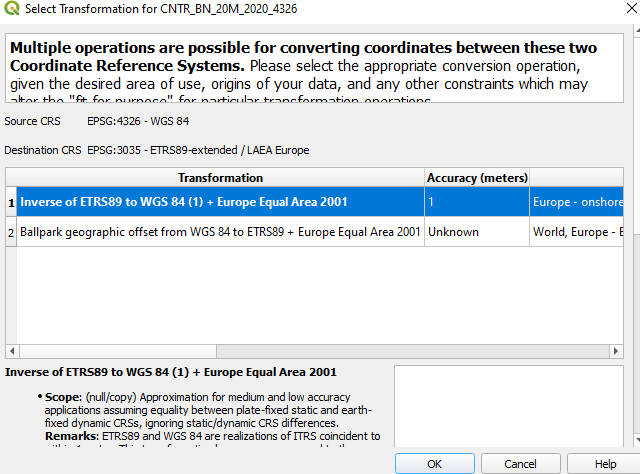
\includegraphics{images/lab_2/lab_2_img_5_crs_warning.png}

\begin{enumerate}
\def\labelenumi{(\arabic{enumi})}
\setcounter{enumi}{53}
\tightlist
\item
  Look at the shape of the UK again after changing the project CRS. Then
  right click on the layer name and select ``Zoom to Layer(s).''
\end{enumerate}

\begin{tcolorbox}[enhanced jigsaw, coltitle=black, toprule=.15mm, breakable, opacitybacktitle=0.6, left=2mm, colback=white, leftrule=.75mm, rightrule=.15mm, colbacktitle=quarto-callout-important-color!10!white, toptitle=1mm, titlerule=0mm, colframe=quarto-callout-important-color-frame, arc=.35mm, bottomtitle=1mm, opacityback=0, bottomrule=.15mm, title=\textcolor{quarto-callout-important-color}{\faExclamation}\hspace{0.5em}{Stop and Think}]

\begin{enumerate}
\def\labelenumi{\alph{enumi})}
\item
  How does the rest of the world look now? Why?
\item
  When you move your mouse, what unit are the coordinates in?
\end{enumerate}

\end{tcolorbox}

\begin{tcolorbox}[enhanced jigsaw, toprule=.15mm, breakable, left=2mm, colframe=quarto-callout-important-color-frame, colback=white, arc=.35mm, leftrule=.75mm, opacityback=0, rightrule=.15mm, bottomrule=.15mm]

\vspace{-3mm}\textbf{Click for answer}\vspace{3mm}

\begin{enumerate}
\def\labelenumi{\alph{enumi})}
\item
  As you move further away from the centre of the projection, shape gets
  progressively more distorted. This is because the LAEA projection is
  only conformal at its centre. But areas are all correct.
\item
  In metres. You can check that on the layer's
  \texttt{Properties\ \textgreater{}\ Information} tab.
\end{enumerate}

\end{tcolorbox}

\begin{enumerate}
\def\labelenumi{(\arabic{enumi})}
\setcounter{enumi}{54}
\tightlist
\item
  Now add to the project the file called
  CNTR\_BN\_20M\_2024\_3035.geojson. Notice the different last four
  numbers on the file name.
\end{enumerate}

\begin{tcolorbox}[enhanced jigsaw, coltitle=black, toprule=.15mm, breakable, opacitybacktitle=0.6, left=2mm, colback=white, leftrule=.75mm, rightrule=.15mm, colbacktitle=quarto-callout-important-color!10!white, toptitle=1mm, titlerule=0mm, colframe=quarto-callout-important-color-frame, arc=.35mm, bottomtitle=1mm, opacityback=0, bottomrule=.15mm, title=\textcolor{quarto-callout-important-color}{\faExclamation}\hspace{0.5em}{Stop and Think}]

What is the CRS for this new layer, and how well does it visually align
with the previous layer?

\end{tcolorbox}

\begin{tcolorbox}[enhanced jigsaw, toprule=.15mm, breakable, left=2mm, colframe=quarto-callout-important-color-frame, colback=white, arc=.35mm, leftrule=.75mm, opacityback=0, rightrule=.15mm, bottomrule=.15mm]

\vspace{-3mm}\textbf{Click for answer}\vspace{3mm}

This second layers uses the EPSG 3035 CRS, while the previous layer used
EPSG 4326. Notice how each layer maintains its original CRS when added
to the project, but if necessary they are reprojected `on the fly' to
match up visually.

\end{tcolorbox}

\begin{enumerate}
\def\labelenumi{(\arabic{enumi})}
\setcounter{enumi}{55}
\item
  Change the project CRS back to EPSG:4326.
\item
  Now go back to the project CRS properties and check the box that says
  \texttt{No\ CRS} at the top of the window. This disables the
  on-the-fly projection. Then click OK and go back to your map.
\item
  Right click on the 4326 layer and select \texttt{Zoom\ to\ Layer}.
  Then select the zoom out tool (the loupe with a minus sign) at the top
  button row, and start clicking at the centre of the map. Keep clicking
  as it gets really small - you should click about 17 times until the
  second dataset is fully visible. Check the properties of each layer to
  make sure they still have the same CRS of when you loaded them.
\end{enumerate}

\begin{tcolorbox}[enhanced jigsaw, coltitle=black, toprule=.15mm, breakable, opacitybacktitle=0.6, left=2mm, colback=white, leftrule=.75mm, rightrule=.15mm, colbacktitle=quarto-callout-important-color!10!white, toptitle=1mm, titlerule=0mm, colframe=quarto-callout-important-color-frame, arc=.35mm, bottomtitle=1mm, opacityback=0, bottomrule=.15mm, title=\textcolor{quarto-callout-important-color}{\faExclamation}\hspace{0.5em}{Stop and Think}]

What has happened? Why are the two datasets suddenly very different in
size?

\end{tcolorbox}

\begin{tcolorbox}[enhanced jigsaw, toprule=.15mm, breakable, left=2mm, colframe=quarto-callout-important-color-frame, colback=white, arc=.35mm, leftrule=.75mm, opacityback=0, rightrule=.15mm, bottomrule=.15mm]

\vspace{-3mm}\textbf{Click for answer}\vspace{3mm}

Since you turned off on-the-fly reprojection, each dataset is now drawn
at their original coordinates - but one is in meters and the other in
degrees, so their x,y positions and scale become very different.

\end{tcolorbox}

\subsection{Potential issues with using mismatched
data}\label{potential-issues-with-using-mismatched-data}

\begin{enumerate}
\def\labelenumi{(\arabic{enumi})}
\setcounter{enumi}{58}
\item
  Download
  \href{https://stir-my.sharepoint.com/:u:/g/personal/ala2_stir_ac_uk/EWwn64TEDgFCvLE-JUwjUZEBMRXc6NKtQ0KWHk769hI4Jw?e=iR9RdT}{this
  vector shapefile (link)}, unzip it and add it to your QGIS project.
  Check what the CRS of this layer is.
\item
  Set the Project CRS back to EPSG:3035. Then go to the top menu bar and
  select
  \texttt{Vector\ \textgreater{}\ Geoprocessing\ \textgreater{}\ Clip}.
  Select the layer that has the EPSG 3035 projection as your
  \texttt{Input} Layer, and the new ``clip\_bounds'' layer as your
  \texttt{Overlay} Layer. You can just leave the output as a temporary
  file. Click Run.
\item
  Turn off the visibility of all layers except the new ``Clipped'' layer
  to see the result of the Clip operation.
\item
  Rename the ``Clipped'' layer to ``Clipped\_3035'' by right clicking on
  it and selecting \texttt{Rename\ layer}. Then repeat the \texttt{Clip}
  operation, this time selecting the 4326 world layer as \texttt{Input},
  and ``clip\_bounds'' as \texttt{Overlay} again. Rename the result to
  ``Clipped\_4326.''
\end{enumerate}

Using what you learned on the previous lab activities, pick two
contrasting colours for each ``Clipped\_\ldots{}'' layer, and make the
lines thicker. Zoom in at the lines of each clipped layer and check if
they overlap perfectly.

\begin{tcolorbox}[enhanced jigsaw, coltitle=black, toprule=.15mm, breakable, opacitybacktitle=0.6, left=2mm, colback=white, leftrule=.75mm, rightrule=.15mm, colbacktitle=quarto-callout-important-color!10!white, toptitle=1mm, titlerule=0mm, colframe=quarto-callout-important-color-frame, arc=.35mm, bottomtitle=1mm, opacityback=0, bottomrule=.15mm, title=\textcolor{quarto-callout-important-color}{\faExclamation}\hspace{0.5em}{Stop and Think}]

Why are the clipping results different even though the initial 3035 and
4236 layers looked perfectly aligned?

\end{tcolorbox}

\begin{tcolorbox}[enhanced jigsaw, toprule=.15mm, breakable, left=2mm, colframe=quarto-callout-important-color-frame, colback=white, arc=.35mm, leftrule=.75mm, opacityback=0, rightrule=.15mm, bottomrule=.15mm]

\vspace{-3mm}\textbf{Click for answer}\vspace{3mm}

Because although they are reprojected `on-the-fly' to visually match on
screen, GIS operations will not take this into consideration when doing
their calculations in the background. As the files still have different
CRSs, this affects the lining up between the \texttt{Input} and
\texttt{Overlay} layers. That is why it is so important to always
permanently translate (reproject) all datasets to the same CRS at the
start of a project.

\end{tcolorbox}

\begin{enumerate}
\def\labelenumi{(\arabic{enumi})}
\setcounter{enumi}{62}
\item
  Now go to
  \texttt{Vector\ \textgreater{}\ Data\ Management\ Tools\ \textgreater{}\ Reproject\ Layer}.
  Select the 4326 world layer as your \texttt{Input\ Layer}, and
  EPSG:3035 as your \texttt{Target\ CRS}. Let the result be a temporary
  file and click \texttt{OK}. The new layer will be automatically named
  as ``Reprojected''. What is the CRS of this new layer (check on the
  layer properties window)?
\item
  Now repeat the use of the \texttt{Clip} tool using ``Reprojected'' as
  the \texttt{Input\ Layer} and ``clip\_bounds'' as the
  \texttt{Overlay\ Layer}. Rename the resulting layer to
  ``Clipped\_Reprojected''. Which of the two originally clipped layers
  (``Clipped\_3035'' or ``Clipped\_4236?) better matches
  the''Clipped\_Reprojected'' layer?
\end{enumerate}

\begin{tcolorbox}[enhanced jigsaw, coltitle=black, toprule=.15mm, breakable, opacitybacktitle=0.6, left=2mm, colback=white, leftrule=.75mm, rightrule=.15mm, colbacktitle=quarto-callout-important-color!10!white, toptitle=1mm, titlerule=0mm, colframe=quarto-callout-important-color-frame, arc=.35mm, bottomtitle=1mm, opacityback=0, bottomrule=.15mm, title=\textcolor{quarto-callout-important-color}{\faExclamation}\hspace{0.5em}{Stop and Think}]

What does the \texttt{Reproject} operation do?

\end{tcolorbox}

\begin{tcolorbox}[enhanced jigsaw, toprule=.15mm, breakable, left=2mm, colframe=quarto-callout-important-color-frame, colback=white, arc=.35mm, leftrule=.75mm, opacityback=0, rightrule=.15mm, bottomrule=.15mm]

\vspace{-3mm}\textbf{Click for answer}\vspace{3mm}

It applies a permanent mathematical transformation to the coordinates of
the input data, translating the data from one CRS to another. For any
GIS project that involves multiple data layers with different CRSs, you
should pick the CRS that makes more sense for your project as the
`project CRS', and then reproject all layers to the same CRS before
anything else.

\end{tcolorbox}

This is the end of Lab 2! You should now understand why different
datasets may have different Coordinate Reference Systems, what the
problems are with working with data that has mismatched CRSs, and how to
reproject data to match a given CRS. As this is your first week, there
are no additional independent exercises - let's take it easy!

If you still want to practice more, check the exercises from the
\href{https://docs.qgis.org/3.34/en/docs/training_manual/basic_map/index.html}{QGIS
Training Manual}!

\part{Week 2 - Vector data}

In our second week, we will take a deeper dive into understanding GIS
spatial vector data. This is the most common data model you will
encounter while working with GIS, so make sure you take your time to
understand it fully.

\section*{ILOs covered}\label{ilos-covered-1}
\addcontentsline{toc}{section}{ILOs covered}

\markright{ILOs covered}

\begin{enumerate}
\def\labelenumi{\arabic{enumi}.}
\item
  Understand the structure of spatial data and choose appropriate data
  types and models for storing and representing it;
\item
  Obtain and assess the quality of spatial data from online and offline
  sources and produce new spatial data using computer and field methods;
\item
  Create map visualisations that adhere to cartographic principles and
  can be easily and unambiguously interpreted by the non-specialist
  public;
\item
  Plan and execute GIS analytical steps to solve spatial problems
  successfully;
\end{enumerate}

\section*{What will you learn}\label{what-will-you-learn-1}
\addcontentsline{toc}{section}{What will you learn}

\markright{What will you learn}

Use this list as a `check-list' to gauge your learning for each week. If
you don't feel confident you have learned any specific topic, then
revisit the week's material!

\subsection*{Theoretical knowledge for Week
2:}\label{theoretical-knowledge-for-week-2}
\addcontentsline{toc}{subsection}{Theoretical knowledge for Week 2:}

\begin{itemize}
\tightlist
\item
  What are data models vs data formats (file formats) vs data types
  (attribute types)?
\item
  What is the vector data model?

  \begin{itemize}
  \tightlist
  \item
    How are vectors represented?
  \item
    What are the components of a vector file (geometry + attribute)?
  \end{itemize}
\item
  What are the main vector file formats?
\item
  What are the main data types we use to represent attributes?
\item
  What kinds of data can we represent using vector data?
\item
  What kinds of questions can we answer using attributes?
\item
  What kinds of questions can we answer using geometries?
\item
  What kinds of questions can we answer using both (i.e.~geometry-based
  attribute calculations).
\end{itemize}

\subsection*{Practical knowledge:}\label{practical-knowledge-1}
\addcontentsline{toc}{subsection}{Practical knowledge:}

Chapter~\ref{sec-labvec1}

\begin{itemize}
\tightlist
\item
  How to identify a vector file format
\item
  How to load a vector file
\item
  How to use the identify tool to get information on the fly
\item
  The concept of `selecting' a feature.
\item
  How to select features using the click tools in QGIS
\item
  How to access the attribute table
\item
  How to use the statistical summary tool

  \begin{itemize}
  \tightlist
  \item
    Global summaries vs summaries on selected data
  \end{itemize}
\item
  How to select using simple queries (filter) on attributes

  \begin{itemize}
  \tightlist
  \item
    Boolean operators
  \item
    String based operators
  \end{itemize}
\item
  How to use attributes to set symbology

  \begin{itemize}
  \tightlist
  \item
    Single symbol
  \item
    Categorised
  \item
    Graduated
  \end{itemize}
\end{itemize}

Chapter~\ref{sec-labvec2}

\begin{itemize}
\tightlist
\item
  How to do combined attribute queries (AND / OR)
\item
  How to calculate new attributes

  \begin{itemize}
  \tightlist
  \item
    Numeric attributes
  \item
    String attributes
  \item
    Geometry attributes\\
  \end{itemize}
\item
  How to convert data types if needed
\item
  Attribute selection vs attribute filtering
\item
  How to select based on location

  \begin{itemize}
  \tightlist
  \item
    The different selection options
  \item
    Importance of CRS matching
  \item
    Select by location vs clipping -How to combine spatial and attribute
    selection
  \item
    Selecting within selections or saving intermediate results
  \end{itemize}
\end{itemize}

\chapter{Lab 3: Working with vector attributes}\label{sec-labvec1}

Vector data consists of discrete observations called features. For
example, on a vector layer representing all protected areas in Scotland,
each individual protected area would comprise a feature. With regular
data, observations are just rows on a table, but with vector spatial
data, features are composed of two elements: the geometry (the visual
component + coordinates) and attributes (columns on a table holding data
about each feature, also known as \emph{fields}).

On the figure below, each country is a feature - the shape of the
country is represented by the geometry (left) and the corresponding
\emph{attributes} are shown in the right. Notice that both the geometry
and the corresponding attributes of one specific feature (Brazil) are
\emph{selected}. Selections are a very important component of GIS
analysis, as they can narrow down the targets for your calculations.

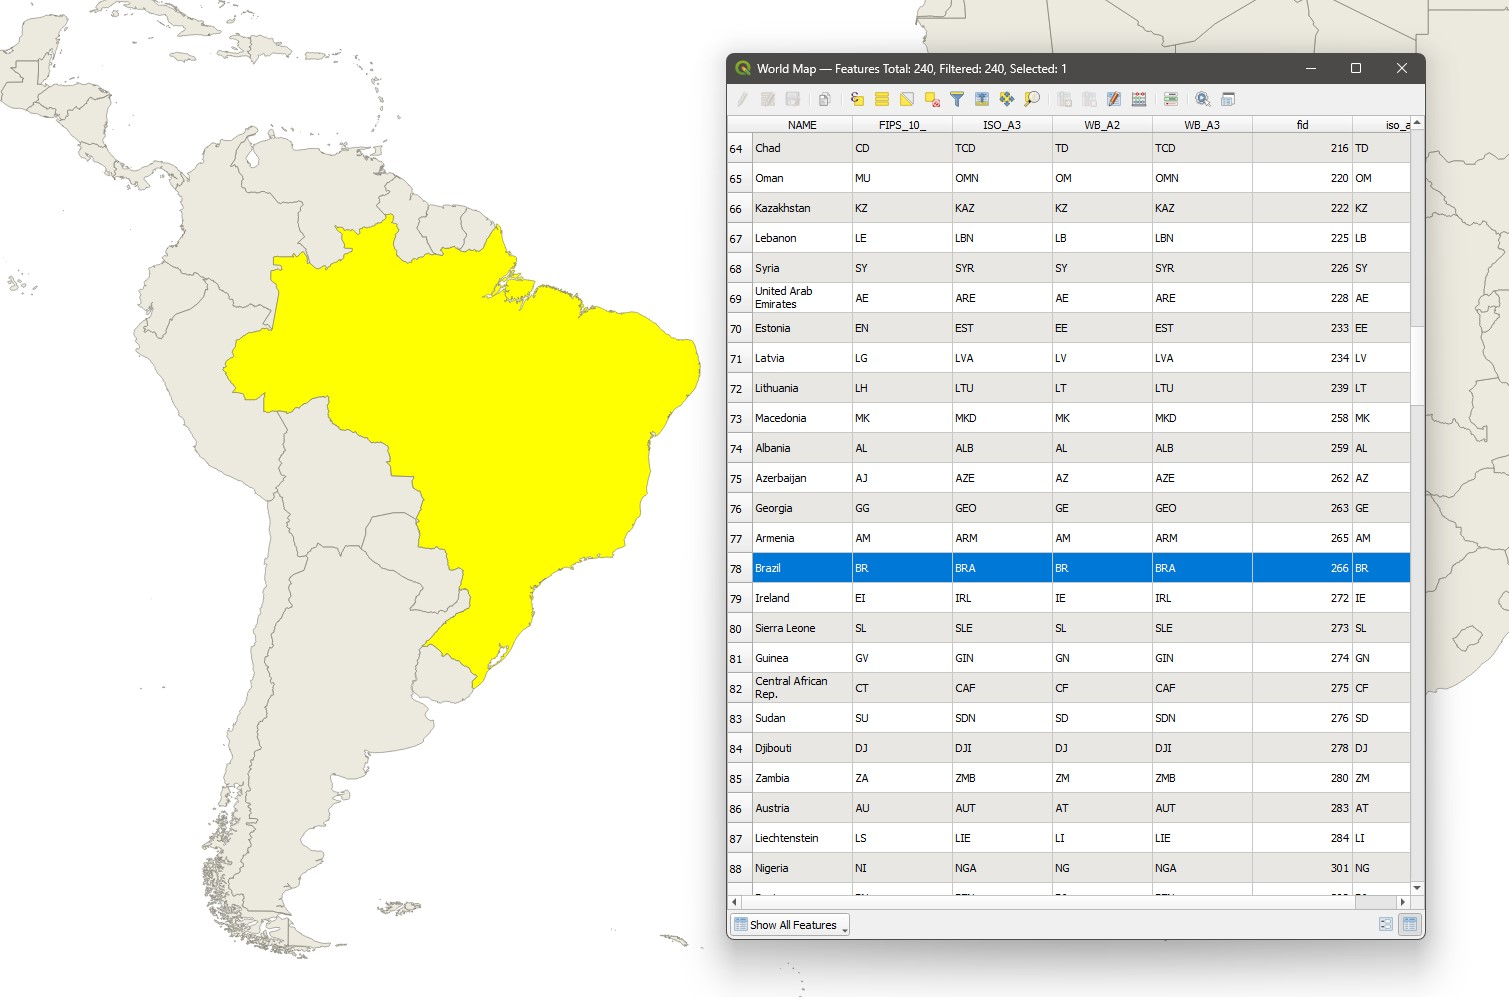
\includegraphics{images/lab_3/lab3_fig1_geometries+attributes.jpg}

For this lab, we will focus mainly on the following GIS operations:
filtering attributes, summarising attributes, and creating and modifying
attribute data. Remember to apply, from here on, all the steps you have
already learned in previous labs: create a project folder, organize your
data, save a named project with proper CRS info, etc. Each week's labs
will build upon the previous activities, so I will not be repeating
instructions for things covered in previous sessions.

\section{Before you start!}\label{before-you-start-1}

\begin{enumerate}
\def\labelenumi{\arabic{enumi}.}
\tightlist
\item
  Go through the Week 2 preparatory session on Canvas, and watch the
  seminar recording if you have missed it.
\end{enumerate}

\section{Guided Exercise 1 - Basic work with Vector
Data}\label{guided-exercise-1---basic-work-with-vector-data}

In this exercise, you will learn how to open and read vector data.

\begin{enumerate}
\def\labelenumi{(\arabic{enumi})}
\setcounter{enumi}{64}
\item
  \href{https://stir-my.sharepoint.com/:f:/g/personal/ala2_stir_ac_uk/EkD-gndA8ihElmcQFirYbPEBN6qvH2tzyLgJ8UujpCXi2Q?e=tsvmoG}{Download
  the data for this exercise from here}, then extract the zip files
  (make sure all the data are unzipped! Sometimes you have zipfiles
  inside zipfiles\ldots) and organise them to your preference (use a
  similar folder structure as from week 1).
\item
  Load all three datasets in QGIS and inspect them. The file names are:
  \texttt{global\_earthquakes\_2011.gpkg}, \texttt{MajorRivers.shp}, and
  \texttt{ne\_50m\_admin\_0\_countries.shp}.
\end{enumerate}

\begin{tcolorbox}[enhanced jigsaw, coltitle=black, toprule=.15mm, breakable, opacitybacktitle=0.6, left=2mm, colback=white, leftrule=.75mm, rightrule=.15mm, colbacktitle=quarto-callout-important-color!10!white, toptitle=1mm, titlerule=0mm, colframe=quarto-callout-important-color-frame, arc=.35mm, bottomtitle=1mm, opacityback=0, bottomrule=.15mm, title=\textcolor{quarto-callout-important-color}{\faExclamation}\hspace{0.5em}{Stop and Think}]

\begin{enumerate}
\def\labelenumi{\alph{enumi})}
\item
  What are the datasets you have?
\item
  What are the \emph{data models} used by these datasets?
\item
  What are the \emph{file formats} you have to work with?
\item
  Which of these files contain \emph{metadata} about your datasets?
\item
  What is the \emph{CRS} of each data layer you have?
\end{enumerate}

\end{tcolorbox}

\begin{tcolorbox}[enhanced jigsaw, toprule=.15mm, breakable, left=2mm, colframe=quarto-callout-important-color-frame, colback=white, arc=.35mm, leftrule=.75mm, opacityback=0, rightrule=.15mm, bottomrule=.15mm]

\vspace{-3mm}\textbf{Click for answer}\vspace{3mm}

\begin{enumerate}
\def\labelenumi{\alph{enumi})}
\item
  You can use the file names, the metadata, and the visual appearance of
  the layers to answer data. The \texttt{global\_earthquakes\_2011.gpkg}
  file seems to hold point data on recorded Earthquake locations in the
  year 2011. The \texttt{MajorRivers.shp} layer seems to hold line data
  on the world's largest rivers. The
  \texttt{ne\_50m\_admin\_0\_countries.shp} seems to have boundaries for
  the world countries.
\item
  All three files use the \emph{vector} data model, being a point
  vector, line vector and polygon vector respectively.
\item
  The earthquakes layer is given in the
  \href{https://www.geopackage.org/}{geopackage} file format, while the
  other two layers are given in the
  \href{https://doc.arcgis.com/en/arcgis-online/reference/shapefiles.htm}{shapefile}
  file format. Notice that data model and file format are two different
  things, and they don't necessarily imply each other. Geopackages, for
  example, can hold both \emph{vector} and \emph{raster} data.
\item
  The rivers layer has a plain text metadata file with a link that
  points to the source of the data, where more information can be found.
  The countries layer has an HTML file that holds metadata about the
  file. The earthquakes data has no metadata.
\item
  All three layers are using EPSG 4236 (WGS84 `unprojected') as CRS. You
  check it by right clicking on the layer name and selecting
  \texttt{Layer\ CRS}, or by selecting
  \texttt{Properties\ \textgreater{}\ Information}.
\end{enumerate}

\end{tcolorbox}

\begin{enumerate}
\def\labelenumi{(\arabic{enumi})}
\setcounter{enumi}{66}
\item
  Check your Project properties to make sure they are correct (does the
  project CRS match the layers? What are the measurement units set for
  this project? Have you set the base folder?). Then save your project
  file within your folder structure as in previous labs.
\item
  Now inspect the \emph{attribute table} for each layer, by
  right-clicking on each layer name and then on
  \texttt{Open\ Attribute\ Table}. Then answer the following questions:
\end{enumerate}

\begin{tcolorbox}[enhanced jigsaw, coltitle=black, toprule=.15mm, breakable, opacitybacktitle=0.6, left=2mm, colback=white, leftrule=.75mm, rightrule=.15mm, colbacktitle=quarto-callout-important-color!10!white, toptitle=1mm, titlerule=0mm, colframe=quarto-callout-important-color-frame, arc=.35mm, bottomtitle=1mm, opacityback=0, bottomrule=.15mm, title=\textcolor{quarto-callout-important-color}{\faExclamation}\hspace{0.5em}{Stop and Think}]

\begin{enumerate}
\def\labelenumi{\alph{enumi})}
\item
  How many \emph{features} does each layer have?
\item
  How many \emph{attributes} does each feature have?
\end{enumerate}

Tip: if you go to \texttt{Properties\ \textgreater{}\ Fields}, you get a
list of all attributes ordered by ID, which is a sequential number. That
makes it easier to count attributes when there are many.

\end{tcolorbox}

\begin{tcolorbox}[enhanced jigsaw, toprule=.15mm, breakable, left=2mm, colframe=quarto-callout-important-color-frame, colback=white, arc=.35mm, leftrule=.75mm, opacityback=0, rightrule=.15mm, bottomrule=.15mm]

\vspace{-3mm}\textbf{Click for answer}\vspace{3mm}

\begin{enumerate}
\def\labelenumi{\alph{enumi})}
\item
  Earthquakes: 15272; Rivers: 98; Countries: 241.
\item
  Earthquakes: 5 (fid, Event, latitude, longitude, Magnitude, Date);
  Rivers: 4 (NAME, SYSTEM, MILES, KILOMETERS); Countries: 94
  (featurecla, scalerank, etc\ldots).
\end{enumerate}

If you looked at \texttt{Properties\ \textgreater{}\ Fields}, the last
ID is 93, but the first one is 0, so 94 in total.

\end{tcolorbox}

\begin{enumerate}
\def\labelenumi{(\arabic{enumi})}
\setcounter{enumi}{68}
\item
  Rename your layers on the layer list to human-readable, informative
  names, then save your project. Remember, these new names will appear
  within this project only, the name of the source files in your folders
  will not change.
\item
  Organize the layer order and play with different layer superpositions
  to make the most readable visualisation for all datasets involved.
  Then experiment with the symbology of each layer to improve your
  visualization.
\end{enumerate}

\section{Guided Exercise 2: Visualising layer
attributes}\label{guided-exercise-2-visualising-layer-attributes}

One of the main applications of vector data is the ability to
\emph{select} and then \emph{summarise} the different attributes of each
layer to extract relevant information.

\begin{enumerate}
\def\labelenumi{(\arabic{enumi})}
\setcounter{enumi}{70}
\item
  Turn off the ``Rivers'' and ``Earthquakes'' layers. (Tip: to turn
  multiple layers off or on at once, highlight all the layers you need
  to make hidden (or visible) by holding down the \texttt{Control} key
  of your keyboard while you click, then hit the spacebar on your
  keyboard).
\item
  Go to \texttt{Layer\ Properties\ \textgreater{}\ Symbology} for the
  World Countries layer, and change the top option from
  \texttt{Single\ Symbol} to \texttt{Categorized}. This lets you assign
  different colours based on attribute values. We will colour the
  countries based on the main region where they are. For \texttt{Value},
  choose the \texttt{REGION\_UN} attribute. Leave the \texttt{Symbol}
  option as is, and for \texttt{Color\ Ramp}, select
  \texttt{Random\ Colors} if it is not already. Then click on the
  \texttt{Classify} button on the bottom left of the large white space
  in the middle of the window. Then click on \texttt{OK}.
\item
  Look at your layer and notice how it has been styled. Try to manually
  change the colours of each region to your liking.
\end{enumerate}

Now let's use visualisation to understand the distribution of world
population.

\begin{enumerate}
\def\labelenumi{(\arabic{enumi})}
\setcounter{enumi}{73}
\item
  Return to the \texttt{Symbology} window and select \texttt{Graduated}
  instead of \texttt{Categorized}. Change your \texttt{Value} to the
  \texttt{POP\_EST} attribute. Choose \texttt{Magma} as your colour ramp
  (click on the little arrow to the right), and select the
  \texttt{Invert\ Color\ Ramp} option.
\item
  Change the classification \texttt{Mode} (above the classify button) to
  \texttt{Equal\ interval}, leave the number of \texttt{Classes} as 5
  (to the left of \texttt{Mode}), and then click on \texttt{Classify},
  then \texttt{OK}.
\end{enumerate}

\begin{tcolorbox}[enhanced jigsaw, coltitle=black, toprule=.15mm, breakable, opacitybacktitle=0.6, left=2mm, colback=white, leftrule=.75mm, rightrule=.15mm, colbacktitle=quarto-callout-important-color!10!white, toptitle=1mm, titlerule=0mm, colframe=quarto-callout-important-color-frame, arc=.35mm, bottomtitle=1mm, opacityback=0, bottomrule=.15mm, title=\textcolor{quarto-callout-important-color}{\faExclamation}\hspace{0.5em}{Stop and Think}]

\begin{enumerate}
\def\labelenumi{\alph{enumi})}
\item
  What is the difference between the \texttt{Categorized} and
  \texttt{Graduated} options?
\item
  Does the \texttt{Equal\ Interval} classification give a good
  visualization of the distribution of world population?
\end{enumerate}

\end{tcolorbox}

\begin{tcolorbox}[enhanced jigsaw, toprule=.15mm, breakable, left=2mm, colframe=quarto-callout-important-color-frame, colback=white, arc=.35mm, leftrule=.75mm, opacityback=0, rightrule=.15mm, bottomrule=.15mm]

\vspace{-3mm}\textbf{Click for answer}\vspace{3mm}

\begin{enumerate}
\def\labelenumi{\alph{enumi})}
\item
  \texttt{Categorized} is for \emph{categorical}, non-numeric variables
  (i.e.~names, classes, etc.). \texttt{Graduated} is for
  \emph{continuous} variables (i.e.~quantities, measurements).
\item
  No, because China, India and to a lesser extent the US have much
  larger population numbers than the rest, which biases the breakpoints.
  We will fix it in the next step.
\end{enumerate}

\end{tcolorbox}

\begin{enumerate}
\def\labelenumi{(\arabic{enumi})}
\setcounter{enumi}{75}
\tightlist
\item
  Return to the \texttt{Symbology} window, and change the \texttt{Mode}
  from \texttt{Equal\ Interval} to \texttt{Natural\ Breaks\ (Jenks)},
  and increase the number of \texttt{Classes} to 10. Click on
  \texttt{OK}.
\end{enumerate}

When you are mapping your own data, make sure you explore the different
methods for calculating breakpoints, and also play with the number of
classes. You can see the full explanation of each \texttt{Mode} on the
\href{https://docs.qgis.org/3.34/en/docs/user_manual/working_with_vector/vector_properties.html\#graduated-renderer}{QGIS
Documentation}.

\section{Guided Exercise 3: Selections based on layer
attributes}\label{guided-exercise-3-selections-based-on-layer-attributes}

Now we will look into using \emph{expressions} to search and select
specific features according to their attributes. As GIS vector data
emerged from the database world, these searches as sometimes refereed to
as \emph{queries}.

\begin{enumerate}
\def\labelenumi{(\arabic{enumi})}
\setcounter{enumi}{76}
\item
  Change the symbology of the Countries layer to
  \texttt{Single\ Symbol}, and pick a dark grey. Then turn on the Rivers
  layer, change its symbology to a light blue, and make sure it is on
  top of the Countries layer.
\item
  Open the Rivers layer attribute table (right click on its name then on
  \texttt{Open\ attribute\ table}). Then click on the
  \texttt{Select\ features\ using\ expression} button
  (
\includegraphics{index_files/mediabag/mIconExpressionSelec.png}). You
  will see a new window with three panels, like the one below. If you
  only see two panels, then click on \texttt{Show\ help}:
\end{enumerate}

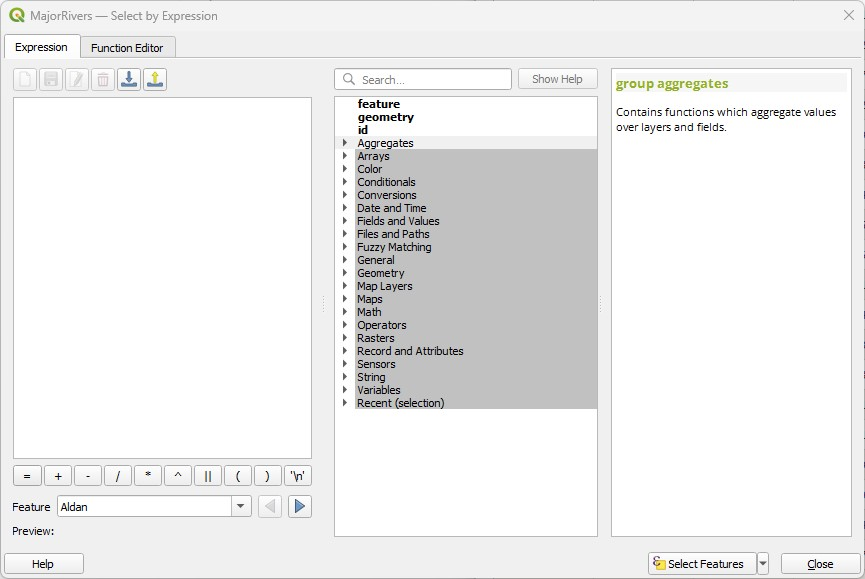
\includegraphics{images/lab_3/lab3_fig2_select_feat_exp.jpg}

You will encounter this expression window in other parts of QGIS as
well. The way it works is that you type your expression on the left
window, using the middle and right panels to browse and select operators
to add to your expression. It will make more sense with an example:

\begin{enumerate}
\def\labelenumi{(\arabic{enumi})}
\setcounter{enumi}{78}
\item
  In the middle panel, expand the \texttt{Fields\ and\ Values} item and
  then double click on \texttt{KILOMETERS}. It will add this attribute
  name to the left panel. Notice that it is enclosed by double quotes.
  In the expression window, \textbf{any word between double quotes means
  it is an attribute's name}. You can also type names directly in the
  window if you prefer, and QGIS will offer autocomplete suggestions
  based on the existing attributes.
\item
  Now complete the expression by typing the remainder, so that the final
  expression is \texttt{"KILOMETERS"\ \textgreater{}\ 5000}. This
  expression means ``Select all River features that have a length -
  represented by the KILOMETERS attribute - larger than 5000''. Then
  click on the \texttt{Select\ features} button.
\item
  Check the results of your selection on the Attribute Table. The number
  of selected features should be shown on the top of the window (11),
  and selected features will be highlighted in blue. On the bottom left
  of the window, you can change from \texttt{Show\ all\ features} to
  \texttt{Show\ selected\ features} if you only want to see the selected
  features.
\item
  Also check the results of your selection on the Map canvas. All
  selected features will be highlighted in yellow. Tip: if you ever set
  the symbology of a feature yellow, remember to not confuse it with
  selected objects. When in doubt, check the attribute table.
\end{enumerate}

\begin{tcolorbox}[enhanced jigsaw, coltitle=black, toprule=.15mm, breakable, opacitybacktitle=0.6, left=2mm, colback=white, leftrule=.75mm, rightrule=.15mm, colbacktitle=quarto-callout-important-color!10!white, toptitle=1mm, titlerule=0mm, colframe=quarto-callout-important-color-frame, arc=.35mm, bottomtitle=1mm, opacityback=0, bottomrule=.15mm, title=\textcolor{quarto-callout-important-color}{\faExclamation}\hspace{0.5em}{Stop and Think}]

It seems the selection is missing a few of the longest rivers in the
world, such as the Amazon River. Why would that be?

Hint: try to use the manual selection tool
(
\includegraphics{index_files/mediabag/mActionSelectRectang.png}) to
click on the Amazon River and investigate.

\end{tcolorbox}

\begin{tcolorbox}[enhanced jigsaw, toprule=.15mm, breakable, left=2mm, colframe=quarto-callout-important-color-frame, colback=white, arc=.35mm, leftrule=.75mm, opacityback=0, rightrule=.15mm, bottomrule=.15mm]

\vspace{-3mm}\textbf{Click for answer}\vspace{3mm}

The different segments of the Amazon River officially receive different
names: Amazonas (lower Amazon), Solimões (central Amazon) and Ucayali
(upper Amazon). In this dataset, it is broken down into two features:
Amazon (with 3042 km) and Ucayali (with 2088 km). Since these are two
separate features, neither is selected by our expression.

\end{tcolorbox}

\begin{enumerate}
\def\labelenumi{(\arabic{enumi})}
\setcounter{enumi}{82}
\tightlist
\item
  Return to the attribute table and make sure that the rivers larger
  than 5000km are still selected. Then create a new expression:
  \texttt{SYSTEM"\ =\ \textquotesingle{}Amazon\textquotesingle{}}.
  Notice that we enclose the word Amazon with single quotes. This
  identifies this as a \emph{string}, i.e.~a character value (like a
  word) within an attribute, and differentiates it from an attribute
  name. Then instead of clicking on \texttt{Select\ Features}, click on
  the small arrow to the right and click in
  \texttt{Add\ to\ Current\ Selection}. Now your selection should
  include all river features that are longer than 5000 km \emph{or}
  belong to the Amazon system (26 features in total).
\end{enumerate}

Tip: If you can't remember all the possible values of an attribute,
select the attribute under \texttt{Fields\ and\ Values} and then on the
right panel, double click on \texttt{All\ Unique}. QGIS will list all
possible value options for that particular attribute.

\begin{enumerate}
\def\labelenumi{(\arabic{enumi})}
\setcounter{enumi}{83}
\tightlist
\item
  Now deselect all features by clicking on the \texttt{Deselect} button
  in the Attribute Table
  (
\includegraphics{index_files/mediabag/mActionDeselectActiv.png}) or
  the \texttt{Deselect\ from\ all\ Layers} button in the main QGIS
  toolbar
  (
\includegraphics{index_files/mediabag/mActionDeselectAll.png}). It is
  always good to clear selections when you are done with a certain
  analysis, to avoid unexpected consequences.
\end{enumerate}

We can use several operators to create expressions. For numeric values,
we can use all logical operators: `greater than'
(\texttt{\textgreater{}}), `lesser than' (\texttt{\textless{}}), their
`or equal' variants (\texttt{\textless{}=}, \texttt{\textgreater{}=}) as
well as `equal' (\texttt{=}) or `not equal'
(\texttt{\textless{}\textgreater{}}). For strings (text), \texttt{=} and
\texttt{\textless{}\textgreater{}} also work, but you can use the
operators \texttt{IS} and \texttt{IS\ NOT} (all upper case) instead. In
the example above, we could have used
\texttt{"SYSTEM"\ IS\ \textquotesingle{}Amazon\textquotesingle{}} to get
the same result.

Another class of useful operators are called \emph{Boolean} operators:
\texttt{AND}, \texttt{OR} and \texttt{NOT}. They allow us to create
compound expressions with multiple criteria:

\begin{enumerate}
\def\labelenumi{(\arabic{enumi})}
\setcounter{enumi}{84}
\item
  Return to the attribute table and this time use the following
  expression:
  \texttt{"KILOMETERS"\ \textgreater{}\ 5000\ OR\ "SYSTEM"\ =\ \textquotesingle{}Amazon\textquotesingle{}}.
  You should get the same results as when you used two separate
  selections with \texttt{Add\ to\ Current\ Selection}. But boolean
  operators can be more powerful.
\item
  Clear your selection and create a new one with the expression
  \texttt{"KILOMETERS"\ \textgreater{}\ 1000\ AND\ "SYSTEM"\ =\ \textquotesingle{}Amazon\textquotesingle{}}.
  When you use the \texttt{AND} operator, each feature must fulfil
  \emph{both} criteria (like an intersection in set theory, if you
  remember your maths). When you use the \texttt{OR} keyword, then each
  feature can fulfil \emph{either} criteria (a mathematical
  \emph{union}).
\item
  Now change the expression to
  \texttt{"KILOMETERS"\ \textgreater{}\ 1000\ AND\ "SYSTEM"\ IS\ NOT\ \textquotesingle{}Amazon\textquotesingle{}}
  and see what you get. Do you understand the effect of using the
  \texttt{NOT}operator?
\end{enumerate}

Finally, we have two useful operators for \emph{partial matching} on
strings. They are useful when you need to select based on a subset of
string (word) values of an attribute:

\begin{enumerate}
\def\labelenumi{(\arabic{enumi})}
\setcounter{enumi}{87}
\item
  Clear your selection and create a new one with the expression
  \texttt{"NAME"\ LIKE\ \textquotesingle{}Am\%\textquotesingle{}}. This
  should select all three rivers whose name starts with `Am' (Amazon,
  Amu Darya and Amur). The `\%' symbol in this case is what we call a
  `wildcard', and it means `anything else'.
\item
  Now use the expression
  \texttt{"NAME"\ LIKE\ \textquotesingle{}C\_\_\_\_\textquotesingle{}}
  (four underscores, '\_`). This should select all rivers whose name
  starts with 'C' followed by any four characters (So it picks Congo and
  Chire).
\end{enumerate}

\begin{tcolorbox}[enhanced jigsaw, coltitle=black, toprule=.15mm, breakable, opacitybacktitle=0.6, left=2mm, colback=white, leftrule=.75mm, rightrule=.15mm, colbacktitle=quarto-callout-important-color!10!white, toptitle=1mm, titlerule=0mm, colframe=quarto-callout-important-color-frame, arc=.35mm, bottomtitle=1mm, opacityback=0, bottomrule=.15mm, title=\textcolor{quarto-callout-important-color}{\faExclamation}\hspace{0.5em}{Stop and Think}]

How many rivers would you get if you changed the above expression to
\texttt{"NAME"\ LIKE\ \textquotesingle{}C\%\textquotesingle{}}?

\end{tcolorbox}

\begin{tcolorbox}[enhanced jigsaw, toprule=.15mm, breakable, left=2mm, colframe=quarto-callout-important-color-frame, colback=white, arc=.35mm, leftrule=.75mm, opacityback=0, rightrule=.15mm, bottomrule=.15mm]

\vspace{-3mm}\textbf{Click for answer}\vspace{3mm}

Four (Columbia, Colorado, Congo, Chire). When you use the `\%' wildcard
it means `any amount of any character'.

\end{tcolorbox}

\begin{enumerate}
\def\labelenumi{(\arabic{enumi})}
\setcounter{enumi}{89}
\tightlist
\item
  Finally, create a selection with the expression
  \texttt{"NAME"\ LIKE\ \textquotesingle{}AM\%\textquotesingle{}}
  (notice the upper-case). You won't get any results. Then change the
  expression to
  \texttt{"NAME"\ ILIKE\ \textquotesingle{}AM\%\textquotesingle{}}. You
  should get the same three rivers starting with `Am' again.
\end{enumerate}

\begin{tcolorbox}[enhanced jigsaw, coltitle=black, toprule=.15mm, breakable, opacitybacktitle=0.6, left=2mm, colback=white, leftrule=.75mm, rightrule=.15mm, colbacktitle=quarto-callout-important-color!10!white, toptitle=1mm, titlerule=0mm, colframe=quarto-callout-important-color-frame, arc=.35mm, bottomtitle=1mm, opacityback=0, bottomrule=.15mm, title=\textcolor{quarto-callout-important-color}{\faExclamation}\hspace{0.5em}{Stop and Think}]

What is the difference between \texttt{LIKE} and \texttt{ILIKE}?

\end{tcolorbox}

\begin{tcolorbox}[enhanced jigsaw, toprule=.15mm, breakable, left=2mm, colframe=quarto-callout-important-color-frame, colback=white, arc=.35mm, leftrule=.75mm, opacityback=0, rightrule=.15mm, bottomrule=.15mm]

\vspace{-3mm}\textbf{Click for answer}\vspace{3mm}

The \texttt{LIKE} operator is case sensitive, while \texttt{ILIKE} is
case insensitive.

\end{tcolorbox}

\begin{enumerate}
\def\labelenumi{(\arabic{enumi})}
\setcounter{enumi}{90}
\tightlist
\item
  Before you move on to the next exercise, make sure you clear your
  selection.
\end{enumerate}

\section{Guided Exercise 3: Summarising layer
attributes}\label{guided-exercise-3-summarising-layer-attributes}

The \texttt{Statistical\ Summary\ Tool}
(
\includegraphics{index_files/mediabag/mActionSum.png}) is a quick way
to summarise attribute values, and can be quite powerful when combined
with attribute selections.

\begin{enumerate}
\def\labelenumi{(\arabic{enumi})}
\setcounter{enumi}{91}
\tightlist
\item
  On the main QGIS window, click on the \texttt{Statistical\ Summary}
  tool button. A new panel will open on the bottom left corner of the
  QGIS window.
\end{enumerate}

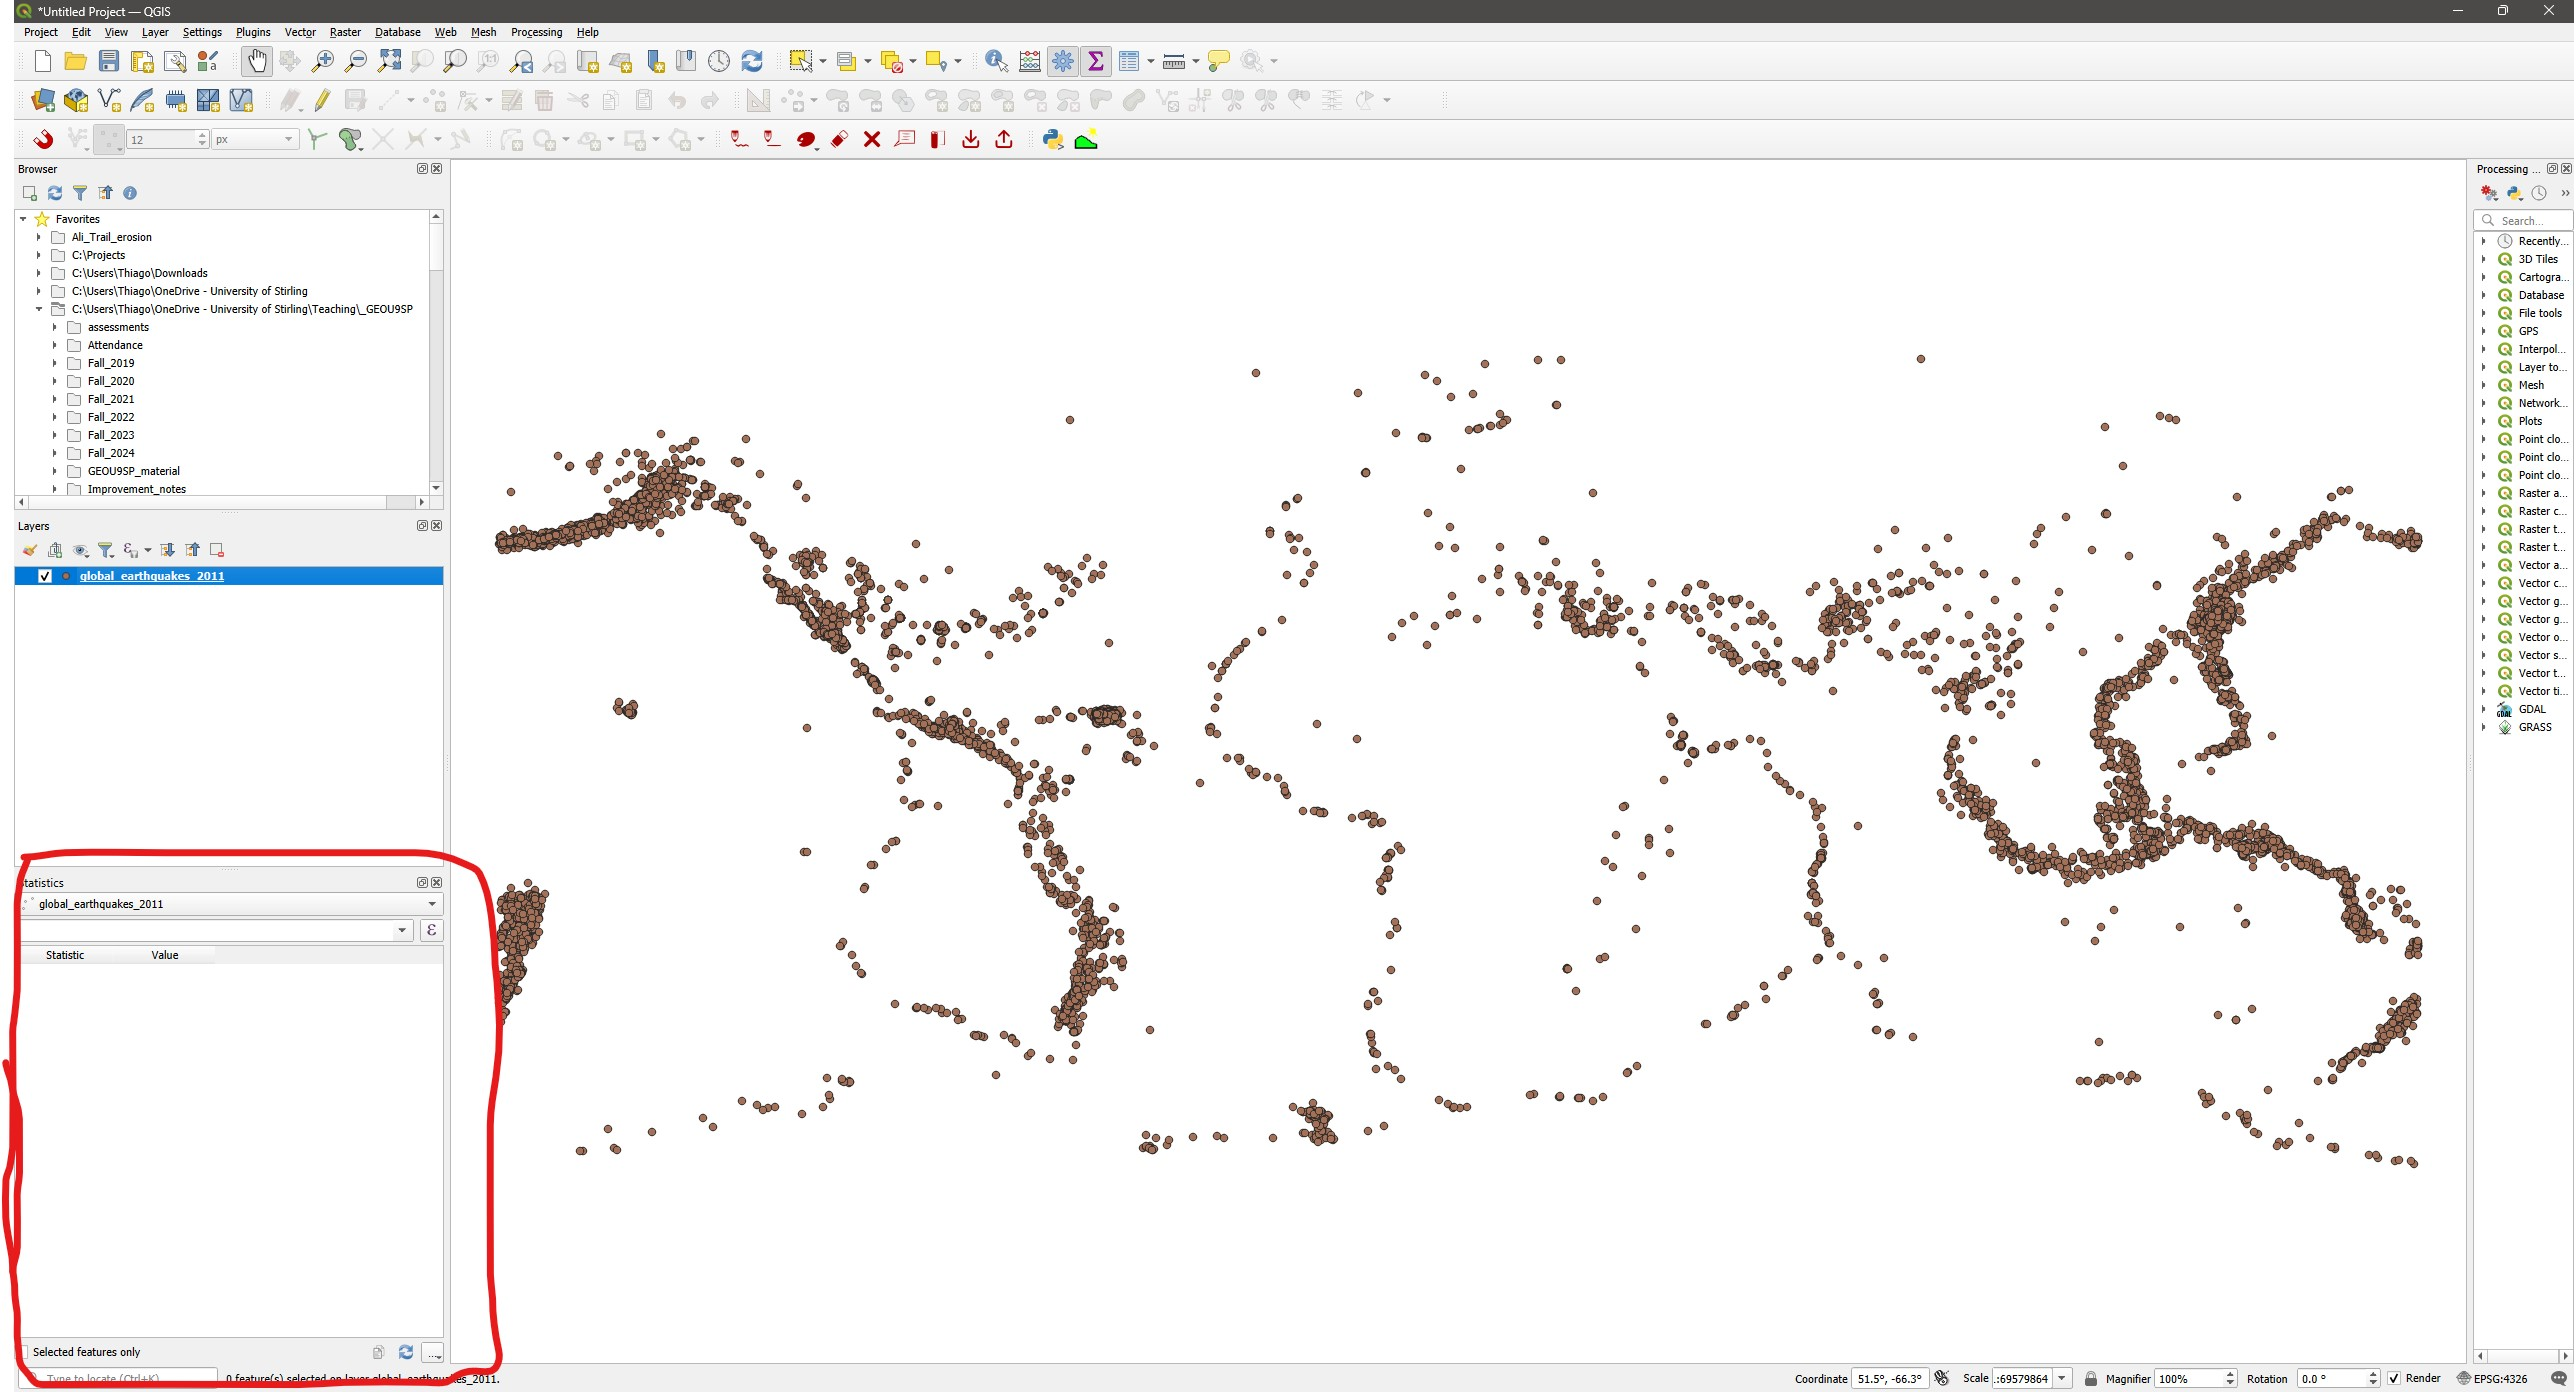
\includegraphics{images/lab_3/lab3_fig4_summ_panel.jpg}

\begin{enumerate}
\def\labelenumi{(\arabic{enumi})}
\setcounter{enumi}{92}
\tightlist
\item
  Select the ``Rivers'' layer as input, then select the
  \texttt{KILOMETERS} attribute on the drop-down menu. You will get a
  table with several summary statistics calculated for all features in
  the layer.
\end{enumerate}

\begin{tcolorbox}[enhanced jigsaw, coltitle=black, toprule=.15mm, breakable, opacitybacktitle=0.6, left=2mm, colback=white, leftrule=.75mm, rightrule=.15mm, colbacktitle=quarto-callout-important-color!10!white, toptitle=1mm, titlerule=0mm, colframe=quarto-callout-important-color-frame, arc=.35mm, bottomtitle=1mm, opacityback=0, bottomrule=.15mm, title=\textcolor{quarto-callout-important-color}{\faExclamation}\hspace{0.5em}{Stop and Think}]

What are the longest, shortest, and mean kilometre lengths in the
dataset?

\end{tcolorbox}

\begin{tcolorbox}[enhanced jigsaw, toprule=.15mm, breakable, left=2mm, colframe=quarto-callout-important-color-frame, colback=white, arc=.35mm, leftrule=.75mm, opacityback=0, rightrule=.15mm, bottomrule=.15mm]

\vspace{-3mm}\textbf{Click for answer}\vspace{3mm}

Max: 9207.1 km; Min: 194.9 km; Mean: 2663.6 km

\end{tcolorbox}

\begin{enumerate}
\def\labelenumi{(\arabic{enumi})}
\setcounter{enumi}{93}
\item
  Now repeat the attribute selection you did before using the expression
  \texttt{"KILOMETERS"\ \textgreater{}\ 5000}, and then return to the
  \texttt{Statistical\ Summary} panel. Then check the
  \texttt{Selected\ Features\ Only} box at the bottom of the window. Now
  the stats will be re-calculated for the selected features only.
\item
  The \texttt{Statistical\ Summary} panel is smart enough to know how to
  summarise different \emph{data types}. For example, select the
  \texttt{SYSTEM} attribute, and see how the stats change - now it gives
  you how many features in total (\texttt{Count}), how many unique
  values (\texttt{Count(Distinct)}), how many missing values
  (\texttt{Count(Missing)}), the \texttt{Minimum} and \texttt{Maximum}
  string values (they don't have a clear meaning here), the least
  (\texttt{Minority}) and most (\texttt{Majority}) common unique values,
  and the \texttt{Minimum\ length} and \texttt{Maximum\ length} in
  number of characters.
\end{enumerate}

\begin{tcolorbox}[enhanced jigsaw, coltitle=black, toprule=.15mm, breakable, opacitybacktitle=0.6, left=2mm, colback=white, leftrule=.75mm, rightrule=.15mm, colbacktitle=quarto-callout-important-color!10!white, toptitle=1mm, titlerule=0mm, colframe=quarto-callout-important-color-frame, arc=.35mm, bottomtitle=1mm, opacityback=0, bottomrule=.15mm, title=\textcolor{quarto-callout-important-color}{\faExclamation}\hspace{0.5em}{Stop and Think}]

Why do you get a blank value for \texttt{Majority} and a 0 for
\texttt{Minimum\ Length}?

\end{tcolorbox}

\begin{tcolorbox}[enhanced jigsaw, toprule=.15mm, breakable, left=2mm, colframe=quarto-callout-important-color-frame, colback=white, arc=.35mm, leftrule=.75mm, opacityback=0, rightrule=.15mm, bottomrule=.15mm]

\vspace{-3mm}\textbf{Click for answer}\vspace{3mm}

For the rivers dataset, \texttt{Majority} is blank and
\texttt{Minimum\ length} is 0 because we have several \texttt{NULL}
(missing) values. They have zero length, and they are in fact the most
common unique value.

\end{tcolorbox}

\section{Guided Exercise 4: Calculating new
attributes}\label{guided-exercise-4-calculating-new-attributes}

Another powerful way to derive information from vector attributes is to
make calculations involving multiple attributes. For that, we can use
the \texttt{Field\ Calculator} tool
(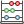
\includegraphics{index_files/mediabag/mActionCalculateFiel.png}),
accessible either from the \texttt{Attribute\ table} or the main QGIS
toolbar.

\begin{enumerate}
\def\labelenumi{(\arabic{enumi})}
\setcounter{enumi}{95}
\item
  Before your start, make sure you clear your selections.
\item
  Go back to the Attribute Table window for the Rivers layer and click
  on the Field Calculator button to open it. It should look like this:
\end{enumerate}

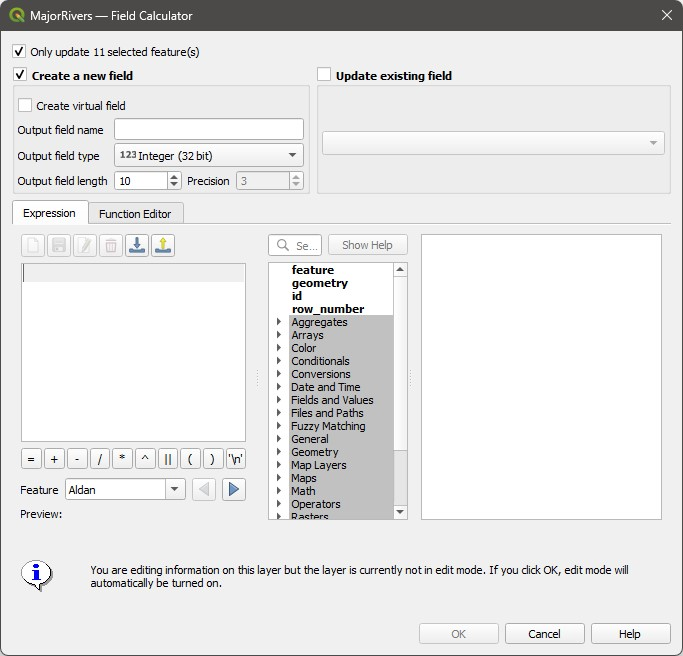
\includegraphics{images/lab_3/lab3_fig3_field_calculator.jpg}

\begin{enumerate}
\def\labelenumi{(\arabic{enumi})}
\setcounter{enumi}{97}
\item
  On the new window, make sure the
  \texttt{Only\ update\ selected\ features} option is \textbf{not}
  checked. Then name the new field \texttt{Mi\_to\_Km}, and change the
  output \emph{data type} to \texttt{Decimal\ Number}.
  \texttt{Output\ field\ length} tells you the maximum number of digits
  that can be stored per attribute value, and the \texttt{Precision}
  field tells you how many of these digits should be decimal places.
\item
  On the expression window, write \texttt{"MILES"\ /\ "KILOMETERS"}.
  Note the warning at the bottom. Now click on \texttt{OK}.
\item
  Now \textbf{turn off editing mode} by clicking on the Toggle Editing
  (
\includegraphics{index_files/mediabag/mActionToggleEditing.png})
  button in the Attribute Table. When asked, confirm you want to save
  the layer changes.
\end{enumerate}

\begin{tcolorbox}[enhanced jigsaw, coltitle=black, toprule=.15mm, breakable, opacitybacktitle=0.6, left=2mm, colback=white, leftrule=.75mm, rightrule=.15mm, colbacktitle=quarto-callout-warning-color!10!white, toptitle=1mm, titlerule=0mm, colframe=quarto-callout-warning-color-frame, arc=.35mm, bottomtitle=1mm, opacityback=0, bottomrule=.15mm, title=\textcolor{quarto-callout-warning-color}{\faExclamationTriangle}\hspace{0.5em}{Warning}]

Turning on editing mode is one of the \textbf{most dangerous} options in
QGIS, as it lets you freely change both the geometry and the attribute
values of a layer. Using the \texttt{Field\ calculator} automatically
puts you on editing mode, so always make sure you turn it off
immediately after you have finished a calculation. Once you make any
changes and then save the changes, \emph{there is no turning back}. I'll
often first export a copy of the layer if I need to do any edits, so I
aways have the original as a backup if something goes wrong. We'll
revisit editing mode on week 4, when we learn how to digitise and edit
geometries by hand.

\end{tcolorbox}

\begin{tcolorbox}[enhanced jigsaw, coltitle=black, toprule=.15mm, breakable, opacitybacktitle=0.6, left=2mm, colback=white, leftrule=.75mm, rightrule=.15mm, colbacktitle=quarto-callout-important-color!10!white, toptitle=1mm, titlerule=0mm, colframe=quarto-callout-important-color-frame, arc=.35mm, bottomtitle=1mm, opacityback=0, bottomrule=.15mm, title=\textcolor{quarto-callout-important-color}{\faExclamation}\hspace{0.5em}{Stop and Think}]

Does the Miles to Km proportion you calculated seem right?

\end{tcolorbox}

\begin{tcolorbox}[enhanced jigsaw, toprule=.15mm, breakable, left=2mm, colframe=quarto-callout-important-color-frame, colback=white, arc=.35mm, leftrule=.75mm, opacityback=0, rightrule=.15mm, bottomrule=.15mm]

\vspace{-3mm}\textbf{Click for answer}\vspace{3mm}

Yes, 1 Mile = 1.609 kilometres.

\end{tcolorbox}

\begin{enumerate}
\def\labelenumi{(\arabic{enumi})}
\setcounter{enumi}{100}
\tightlist
\item
  This new attribute you calculated is not very useful. Let us get rid
  of it. Put the attribute table back into editing mode, then click on
  the \texttt{Delete\ Field} button
  (
\includegraphics{index_files/mediabag/mActionDeleteAttribu.png}), and
  select your \texttt{Mi\_to\_Km} field. Click \texttt{OK}. It's gone!
  Remember to save the changes and exit edit mode.
\end{enumerate}

Tip: if you want to rename an attribute, create a new one with the new
name and just use the name of the old one as the expression on the
\texttt{Field\ Calculator}. It will copy all values to the new
attribute. Then remove the old one.

\begin{enumerate}
\def\labelenumi{(\arabic{enumi})}
\setcounter{enumi}{101}
\tightlist
\item
  We will continue working with this data in the next lab. If you want
  to keep your project, this is the best way to do it: on your
  computer's file explorer, find the root folder for the project
  (\texttt{lab\_3}, or whatever you have named it as). Then right click
  on it and select (on Windows) \texttt{Compress\ to\ Zip\ file}. That
  will create a new zipfile of the folder contents, with the same name
  as the folder. Then you can copy this zip file to your OneDrive folder
  or to an external drive.
\end{enumerate}

Good job, we have now finished our first guided tour of vector
attributes. We will revisit it in the next lab, when we also learn about
geometry-based selections.

Make sure you have a go at the independent exercise below, to make sure
you feel comfortable with attribute selections, calculations and
summaries. You will keep using these skills for the rest of the module
(and your GIS life).

\section{Independent Exercise}\label{independent-exercise}

Using the earthquakes layer you downloaded
(\texttt{global\_earthquakes\_2011.gpkg}), do the following:

\begin{enumerate}
\def\labelenumi{\arabic{enumi})}
\item
  Find out how many earthquakes of magnitude equal or larger than 7 have
  occurred in the Northern Hemisphere in 2011.
\item
  What was the average magnitude of all earthquakes that occurred in
  Japan in 2011? (Tip: make sure you enlarge the \texttt{event} column
  of the attribute table to the whole values).
\item
  Create a new \texttt{Text\ (string)} attribute that indicates if an
  earthquake is located on the western (\texttt{W}) or eastern
  (\texttt{E}) hemisphere.
\end{enumerate}

\chapter{Lab 4: Working with vector geometries}\label{sec-labvec2}

The purpose of this lab is to continue developing your knowledge about
vector spatial data and vector-based GIS operations. Today you will
learn how to make selections based on the overlap of two vector layers -
called spatial selection, location selection or spatial query. This is a
powerful way to combine data from different sources to generate new
information.

\section{Before you start!}\label{before-you-start-2}

\begin{enumerate}
\def\labelenumi{\arabic{enumi}.}
\tightlist
\item
  Go through the Week 2 preparatory session on Canvas, and watch the
  seminar recording if you have missed it. Also make sure you have
  completed Lab 3.
\end{enumerate}

\section{Guided Exercise 1 - Spatial
Queries}\label{guided-exercise-1---spatial-queries}

We will continue with the Earthquakes, Rivers and Countries dataset from
the previous lab.

\begin{enumerate}
\def\labelenumi{(\arabic{enumi})}
\setcounter{enumi}{102}
\tightlist
\item
  If you have zipped your project from the last session, just unzip it
  and get to work. If not, then
  \href{https://stir-my.sharepoint.com/:f:/g/personal/ala2_stir_ac_uk/EkD-gndA8ihElmcQFirYbPEBN6qvH2tzyLgJ8UujpCXi2Q?e=tsvmoG}{download
  the data again}, and redo your project organization. As a reminder,
  the files to be loaded are: \texttt{global\_earthquakes\_2011.gpkg},
  \texttt{MajorRivers.shp}, and
  \texttt{ne\_50m\_admin\_0\_countries.shp}.
\end{enumerate}

For our next step in the analysis, we would like to focus only on
earthquakes on \emph{land} (i.e.~not ocean). This information is not
contained in the Earthquakes layer, but we do have a Countries layer
that separates land from ocean. Could we use that to make a selection?

\begin{enumerate}
\def\labelenumi{(\arabic{enumi})}
\setcounter{enumi}{103}
\tightlist
\item
  Go to the menu
  \texttt{Vector\ \textgreater{}\ Research\ Tools\ \textgreater{}\ Select\ by\ Location...},
  or click on the
  
\includegraphics{index_files/mediabag/mAlgorithmSelectLoca.png} button
  on the main QGIS toolbar. You will get this window:
\end{enumerate}

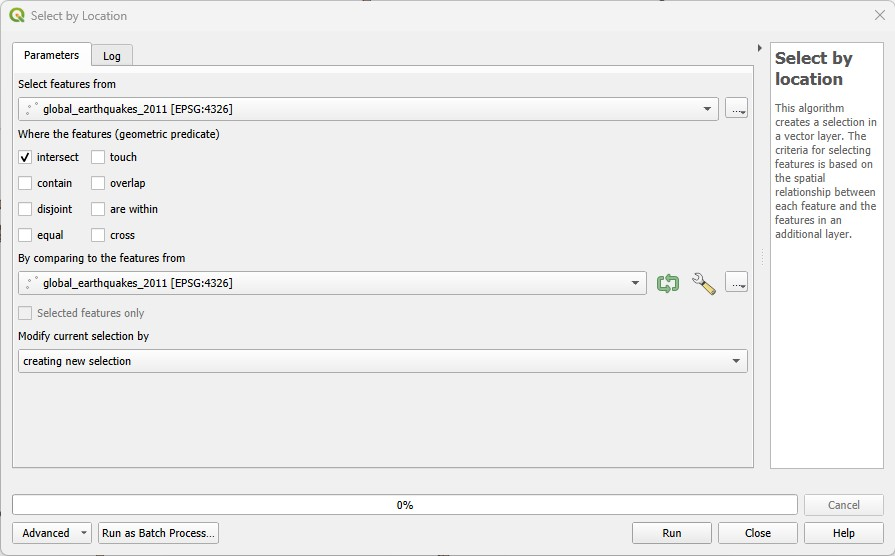
\includegraphics{images/lab_4/lab4_fig1_select_loc.jpg}

\begin{enumerate}
\def\labelenumi{(\arabic{enumi})}
\setcounter{enumi}{104}
\item
  Select the Earthquakes layer as \texttt{Select\ features\ from}. Then
  check \emph{only} the \texttt{Are\ within} query option. Then pick
  your World Countries layer for
  \texttt{By\ comparing\ to\ the\ features\ from}. Click \texttt{Run},
  and after it is finished, click \texttt{Close}.
\item
  Visually inspect the results of your selection, and then open the
  Attribute Table for the Earthquakes layer.
\end{enumerate}

\begin{tcolorbox}[enhanced jigsaw, coltitle=black, toprule=.15mm, breakable, opacitybacktitle=0.6, left=2mm, colback=white, leftrule=.75mm, rightrule=.15mm, colbacktitle=quarto-callout-important-color!10!white, toptitle=1mm, titlerule=0mm, colframe=quarto-callout-important-color-frame, arc=.35mm, bottomtitle=1mm, opacityback=0, bottomrule=.15mm, title=\textcolor{quarto-callout-important-color}{\faExclamation}\hspace{0.5em}{Stop and Think}]

How many Earthquakes were originated on land in 2011?

\end{tcolorbox}

\begin{tcolorbox}[enhanced jigsaw, toprule=.15mm, breakable, left=2mm, colframe=quarto-callout-important-color-frame, colback=white, arc=.35mm, leftrule=.75mm, opacityback=0, rightrule=.15mm, bottomrule=.15mm]

\vspace{-3mm}\textbf{Click for answer}\vspace{3mm}

3742 earthquakes.

\end{tcolorbox}

Now that we identified the earthquakes on the continents, we may want to
add this information to the Earthquakes layer as an attribute, in case
we need the information later.

\begin{enumerate}
\def\labelenumi{(\arabic{enumi})}
\setcounter{enumi}{106}
\item
  Still on the Attribute Table of the Earthquakes layer, open the
  \texttt{Field\ Calculator}, and create a new \texttt{Text(string)}
  field called \texttt{Origin}. Make sure the option
  \texttt{Only\ update\ selected\ features} \textbf{is} enabled this
  time. Then on the Expression window, just write
  \texttt{\textquotesingle{}Land\textquotesingle{}}. That means the word
  \texttt{Land} will be added as the attribute value for every selected
  feature.
\item
  Now back on the Attribute Table window, click on the
  \texttt{Invert\ Selection} button
  (
\includegraphics{index_files/mediabag/mActionInvertSelecti.png}).
\item
  Return to the \texttt{Field\ Calculator} and this time use the
  \texttt{Update\ Existing\ Field} option to the right, instead of
  \texttt{Create\ a\ new\ field}. Make sure the option
  \texttt{Only\ update\ selected\ features} is still enabled. Pick
  \texttt{Origin} as the field to be updated, and now just write
  \texttt{\textquotesingle{}Ocean\textquotesingle{}} on the Expression
  window. Click \texttt{OK}.
\item
  Now use the \texttt{Origin} attribute to style the colour or shape of
  your Earthquake points differently for land and ocean, using the
  \texttt{Symbology} options. Pick the \texttt{Categorized} symbology
  option at the top, set the \texttt{Value} to the \texttt{Origin}
  attribute, and then \texttt{Classify}.
\end{enumerate}

\begin{tcolorbox}[enhanced jigsaw, coltitle=black, toprule=.15mm, breakable, opacitybacktitle=0.6, left=2mm, colback=white, leftrule=.75mm, rightrule=.15mm, colbacktitle=quarto-callout-important-color!10!white, toptitle=1mm, titlerule=0mm, colframe=quarto-callout-important-color-frame, arc=.35mm, bottomtitle=1mm, opacityback=0, bottomrule=.15mm, title=\textcolor{quarto-callout-important-color}{\faExclamation}\hspace{0.5em}{Stop and Think}]

Do you understand why you did the steps above?

\end{tcolorbox}

\begin{tcolorbox}[enhanced jigsaw, toprule=.15mm, breakable, left=2mm, colframe=quarto-callout-important-color-frame, colback=white, arc=.35mm, leftrule=.75mm, opacityback=0, rightrule=.15mm, bottomrule=.15mm]

\vspace{-3mm}\textbf{Click for answer}\vspace{3mm}

We wanted to create a new string attribute designating an Earthquake as
either \texttt{Ocean} or \texttt{Land}. But the information on where the
Earthquake is depends on whether it overlaps with the Countries layer.
So we need to combine \texttt{select\ by\ location} with the
\texttt{Field\ Calculator}. First we create a selection of land quakes
based on location, and then we add a new field to the Earthquakes layer,
to be filled with the word \texttt{Land}. But since we checked the
\texttt{Only\ update\ selected\ features} option, only the selected
features will be filled, and the rest will remain blank (\texttt{Null}).
We then invert our selection so that only ocean quakes are selected, and
update the existing field by filling in the word \texttt{Ocean} just for
these selected features.

Creating this new attribute adds the possibility of styling the points
by \texttt{Origin}, which would not be possible just based on the
selection.

\end{tcolorbox}

Now, let us find details about earthquake originating on a specific
continent.

\begin{enumerate}
\def\labelenumi{(\arabic{enumi})}
\setcounter{enumi}{110}
\item
  On the World layer, use Attribute selection (as in Exercise 3) to
  select all countries from South America. Then go to
  \texttt{Vector\ \textgreater{}\ Research\ Tools\ \textgreater{}\ Select\ by\ Location...}
  and select all Earthquakes that \texttt{are\ within} the Countries
  layer (same process as above), but this time \emph{make sure you turn
  on the option} \texttt{Selected\ features\ only}.
\item
  Another way to make a selection `permanent' is to export it as a new
  layer. While you still have the above selection on, right-click on the
  Earthquakes layer name and choose
  \texttt{Export\ \textgreater{}\ Save\ selected\ features\ as...}. Name
  your exported file as
  \texttt{Land\_earthquakes\_2011\_south\_america}. Choose an
  appropriate folder to save it within your project structure by
  clicking on the \texttt{...} button to the left of the file name box,
  and select your format of choice (geopackage or shapefile). Click on
  \texttt{OK}. Save your project.
\end{enumerate}

\section{Guided Exercise 2 - Geometry-based attribute
calculations}\label{guided-exercise-2---geometry-based-attribute-calculations}

Another way to relate geometries to attributes is when we want to store
some property of the geometry as an attribute itself, such as area,
length or perimeter. QGIS also has tools for that.

As an example, let us calculate the areas and border length (perimeter)
of all the World's countries.

\begin{enumerate}
\def\labelenumi{(\arabic{enumi})}
\setcounter{enumi}{112}
\tightlist
\item
  Before using any of the geometry-based operators, we need to set up
  our desired units for the project. Go to the menu
  \texttt{File\ \textgreater{}\ Properties...} to open your project
  properties. Then on the \texttt{General} tab, set the
  \texttt{Units\ for\ distance\ measurement} to \texttt{Kilometers} and
  the \texttt{Units\ for\ area\ measurement} to
  \texttt{Square\ Kilometers} (yes, we will use
  \href{https://en.wikipedia.org/wiki/International_System_of_Units}{SI}
  units because we are scientists!).
\end{enumerate}

It is always important to think about your problem before choosing the
units for length and area calculations. In this case, using the default
of meters and squared meters would not make sense for things as large as
countries.

\begin{enumerate}
\def\labelenumi{(\arabic{enumi})}
\setcounter{enumi}{113}
\item
  Now open the Attribute Table for the Countries layer and launch the
  \texttt{Field\ Calculator}. Create a new attribute called
  \texttt{Area\_km2} (it is always a good idea to add the units to the
  name to avoid any confusion) that is a decimal number with two decimal
  places. Then on the centre panel, find and expand the
  \texttt{Geometry} heading, and double click on the \texttt{\$area}
  option to add it to the expression window. Then click on \texttt{OK}
  to calculate the field.
\item
  Remember to deactivate editing mode!
\end{enumerate}

\begin{tcolorbox}[enhanced jigsaw, coltitle=black, toprule=.15mm, breakable, opacitybacktitle=0.6, left=2mm, colback=white, leftrule=.75mm, rightrule=.15mm, colbacktitle=quarto-callout-important-color!10!white, toptitle=1mm, titlerule=0mm, colframe=quarto-callout-important-color-frame, arc=.35mm, bottomtitle=1mm, opacityback=0, bottomrule=.15mm, title=\textcolor{quarto-callout-important-color}{\faExclamation}\hspace{0.5em}{Stop and Think}]

\begin{enumerate}
\def\labelenumi{\alph{enumi})}
\item
  What is the difference between \texttt{\$area} and \texttt{area}?
  Hint: look at the help text on the right panel.
\item
  Why should we use \texttt{\$area} instead of \texttt{area} here?
\end{enumerate}

\end{tcolorbox}

\begin{tcolorbox}[enhanced jigsaw, toprule=.15mm, breakable, left=2mm, colframe=quarto-callout-important-color-frame, colback=white, arc=.35mm, leftrule=.75mm, opacityback=0, rightrule=.15mm, bottomrule=.15mm]

\vspace{-3mm}\textbf{Click for answer}\vspace{3mm}

\begin{enumerate}
\def\labelenumi{\alph{enumi})}
\item
  The \texttt{\$area} operator calculates \texttt{geodesic} area,
  meaning it takes into consideration the curved surface of the
  ellipsoid (defined by the projects CRS). It will also use the units
  specified in the project properties. The \texttt{area} operator will
  calculate \emph{planimetric} area (i.e.~a flat surface) and will
  derive the units from the CRS of the layer.
\item
  Since we are calculating very large areas, geodesic area will be more
  correct than planimetric area (unless the dataset uses an
  \emph{equal-area} map projection). Moreover, the data is in EPSG24326
  (WGS 84), which has degrees as units. If we used \texttt{area} we
  would get areas in squared degrees, which don't make a lot of sense.
\end{enumerate}

\end{tcolorbox}

\begin{enumerate}
\def\labelenumi{(\arabic{enumi})}
\setcounter{enumi}{115}
\tightlist
\item
  Now repeat the process above, and calculate \texttt{Per\_km} as a new
  attribute, using the \texttt{\$perimeter} operator (we use it instead
  of \texttt{perimeter} for the same reason above).
\end{enumerate}

\begin{tcolorbox}[enhanced jigsaw, coltitle=black, toprule=.15mm, breakable, opacitybacktitle=0.6, left=2mm, colback=white, leftrule=.75mm, rightrule=.15mm, colbacktitle=quarto-callout-important-color!10!white, toptitle=1mm, titlerule=0mm, colframe=quarto-callout-important-color-frame, arc=.35mm, bottomtitle=1mm, opacityback=0, bottomrule=.15mm, title=\textcolor{quarto-callout-important-color}{\faExclamation}\hspace{0.5em}{Stop and Think}]

The perimeter/area (PA) ratio is often used as a measurement of polygon
complexity. Can you answer which country has the most complex border in
the world?

\end{tcolorbox}

\begin{tcolorbox}[enhanced jigsaw, toprule=.15mm, breakable, left=2mm, colframe=quarto-callout-important-color-frame, colback=white, arc=.35mm, leftrule=.75mm, opacityback=0, rightrule=.15mm, bottomrule=.15mm]

\vspace{-3mm}\textbf{Click for answer}\vspace{3mm}

Use the \texttt{Field\ Calculator} to calculate areas and perimeters
(you just did), then use it to create a new \texttt{PA\_ratio} attribute
(decimal number) using the expression \texttt{"Per\_km"\ /\ "Area\_km2"}
(assuming these are the attribute names you used). Then use the
\texttt{Summary\ Statistics\ tool} to find the maximum
\texttt{PA\_ratio} value in the dataset (4.592). The use
\texttt{Select\ by\ expression} to select which feature has
\texttt{"PA\_ratio"\ =\ 4.592.\ That\ would\ be\ the\ Vatican!\ \ A\ quicker\ way\ to\ answer\ this\ (that\ only\ works\ for\ min/max\ values)\ is\ to\ click\ on\ the}PA\_ratio`
attribute name on the Attribute Table twice, to sort it in ascending and
then descending order, and then checking which country is the top row
after sorting.

\end{tcolorbox}

Good job! You now know all you need to query, create, delete, update and
summarise attributes. You will use these tools a lot whenever you are
doing any GIS work, so it is important to know them well.

To further solidify your knowledge, do the Independent Exercise below,
which reviews all your learning from the past week and this week.

\section{Independent Exercise - Supporting Wildcat conservation in
Scotland.}\label{independent-exercise---supporting-wildcat-conservation-in-scotland.}

You want to investigate how priority areas for wildcat conservation
(WPAs) overlap with protected areas, and the risk of wildcat roadkill.

For that, obtain the following layers from the
\href{https://opendata.nature.scot/}{NatureScot Open Data Hub}. Get them
in either \emph{shapefile} or \emph{geopackage} format.

\begin{itemize}
\tightlist
\item
  Wildcat Priority Areas (WPA)
\item
  Sites of Special Scientific Interest (SSSI)
\end{itemize}

Then obtain the Open Roads layer for all of the UK from the
\href{https://osdatahub.os.uk/downloads/open}{Ordnance Survey OS Open
Data} hub, also as a \emph{geopackage} (it is a large file and it may
take a while to download).

Finally, obtain the UK country boundaries from the
\href{https://gadm.org/data.html}{Global Administrative Boundaries
(GADM)} hub. Get the \emph{GeoJSON} file at \emph{Level 1} (Level 0 is
the UK border without countries, level 1 is countries, level 2 is
counties/council areas, etc.)

Organize the data and create a new project where you load all four
datasets. Order and style them as you prefer. Then:

\begin{enumerate}
\def\labelenumi{\arabic{enumi})}
\item
  Answer the questions:

  \begin{enumerate}
  \def\labelenumii{\alph{enumii})}
  \tightlist
  \item
    What is the data model of each layer?
  \item
    What is the file format of each layer?
  \item
    What is the CRS of each layer?
  \item
    How many features does the WPA dataset have?
  \item
    How many attributes does the WPA dataset have?
  \end{enumerate}
\item
  The UK boundaries file has a different CRS from the rest, and it also
  contains all countries. Reproject this layer to the same CRS as the
  other layers, and then create a new layer containing the Scotland
  boundary only. Remove the UK layer from the project after that.
\item
  The roads layer covers all of the UK, making it very heavy and slow to
  use. But our analysis concerns Scotland only, so create a new layer
  containing only the road links (lines) inside the Scottish boundaries.
  Remove the full UK layer from the project after that.
\item
  The attribute \texttt{Shape\_Area} of the WPA dataset does not
  indicate any units. It is always useful to have field names that hint
  at the unit for the values, making the data more self-explanatory.
  Recalculate the area of each WPA \emph{in square km}, naming the new
  field `Area\_km2'. Then delete the `Shape\_Area' attribute from the
  dataset to avoid confusion for future users.
\item
  The Sites of Specific Scientific Interest (SSSIs) are a category of
  protected area in Scotland. These may offer additional protection to
  wildcats. Find all the SSSIs that overlap with WPAs, and create a new
  layer containing only these sites. Then calculate the total area of
  these SSSIs.
\item
  A major threat to wildlife is roadkill. Using the OS Open Data Open
  Roads dataset, answer the questions below:

  \begin{enumerate}
  \def\labelenumii{\alph{enumii})}
  \item
    How many road segments overlap with WPAs? (Create a new layer
    containing only, the selected data, to use below).
  \item
    What is the total length of roads within WPAs?
  \item
    Not all roads present the same risk. In the UK, roads are classified
    as:

    \begin{itemize}
    \tightlist
    \item
      Motorways: high-speed expressways typically reserved for longer
      journeys between major cities;
    \item
      A roads: major roads intended to provide large-scale transport
      links;
    \item
      B roads: roads intended to connect different areas, and to feed
      traffic between A roads and smaller roads on the network;
    \item
      Classified Unnumbered -- smaller roads intended to connect
      together unclassified roads with A and B roads, and often linking
      a housing estate or a village to the rest of the network;
    \item
      Unclassified -- local roads intended for local traffic. The vast
      majority (60\%) of roads in the UK fall within this category.
    \end{itemize}
  \end{enumerate}
\end{enumerate}

What is the total length per road class for all roads intersecting WPAs?

You will notice a `problem' with the terms used in the road
classification attribute - its unique values don't match the terms
above. You will need to create a new field called \texttt{class\_fix}
that keeps the classification of \texttt{Motorway} \texttt{A},
\texttt{B}, \texttt{Classified\ Unnumbered} and \texttt{Unclassified}
unchanged, but changes the records labelled as both
\texttt{Not\ Classified} and \texttt{Unknown} to \texttt{Unclassified}.

\begin{enumerate}
\def\labelenumi{\alph{enumi})}
\setcounter{enumi}{3}
\item
  Along with road class, the length of the road segment is also
  important in determining overall traffic speed. To take that into
  consideration, select all roads within WPAs that are of either
  Motorway, A or B class and have 100m or more in length. Create a new
  layer from this selection.
\item
  GIS analyses will almost always have a visual component, as maps are a
  natural way to tell a `spatial story'. To finalise your exercise,
  organise and style your layers to show, in the most readable way
  possible (i.e.~think about orders, line colours, widths and styles,
  fill colours, etc):
\end{enumerate}

\begin{itemize}
\tightlist
\item
  The Scottish boundary;
\item
  The WPAs;
\item
  The boundaries of the SSSIs, distinguishing between those that do and
  do not overlap with WPAs;
\item
  All Scottish roads differentiated by class using line width;
\item
  All the road segments that are Motorways, A or B roads within WPAs
  which are longer than 100m. These should use the same line widths as
  above to differentiate road class but have a different colour from
  other roads.
\end{itemize}

\part{Week 3 - Raster data}

For our third week, we will learn about the second most common data
model for spatial data: raster files. While vectors are good at
representing separated and/or well-defined individual regions, rasters
excel at representing gradual, continuous data such as surface
temperatures or elevations.

\section*{ILOs covered}\label{ilos-covered-2}
\addcontentsline{toc}{section}{ILOs covered}

\markright{ILOs covered}

\begin{enumerate}
\def\labelenumi{\arabic{enumi}.}
\item
  Understand the structure of spatial data and choose appropriate data
  types and models for storing and representing it;
\item
  Obtain and assess the quality of spatial data from online and offline
  sources and produce new spatial data using computer and field methods;
\item
  Create map visualisations that adhere to cartographic principles and
  can be easily and unambiguously interpreted by the non-specialist
  public;
\item
  Plan and execute GIS analytical steps to solve spatial problems
  successfully;
\end{enumerate}

\section*{What will you learn}\label{what-will-you-learn-2}
\addcontentsline{toc}{section}{What will you learn}

\markright{What will you learn}

For every week, we will list the main theoretical and practical learning
goals. Use these as a `checklist' to gauge your learning for each week.
If you don't feel confident you have learned any specific topic, then
revisit the week's material!

\subsection*{Theoretical knowledge for Week
3:}\label{theoretical-knowledge-for-week-3}
\addcontentsline{toc}{subsection}{Theoretical knowledge for Week 3:}

\begin{itemize}
\tightlist
\item
  What is the raster data model?

  \begin{itemize}
  \tightlist
  \item
    How are rasters represented?
  \end{itemize}
\item
  What are the components of a raster file (rows, columns,
  bands/channels, resolution)?
\item
  What are the main raster file formats?
\item
  What data types can rasters represent?
\item
  What kinds of data can we represent using raster data?
\item
  Raster / vector component equivalence
\item
  Raster / vector tool equivalence

  \begin{itemize}
  \tightlist
  \item
    No concept of ` selection'
  \end{itemize}
\item
  What kinds of questions can we answer using rasters?
\item
  How can we transform rasters to vectors and vice-versa

  \begin{itemize}
  \tightlist
  \item
    The concept of raster resampling
  \item
    The concept of raster contrast manipulation
  \end{itemize}
\end{itemize}

\subsection*{Practical knowledge:}\label{practical-knowledge-2}
\addcontentsline{toc}{subsection}{Practical knowledge:}

Chapter~\ref{sec-labras1}

\begin{itemize}
\tightlist
\item
  How to identify raster files
\item
  How to load raster files
\item
  How to get raster properties
\item
  How to reproject raster data
\item
  How to mask rasters
\item
  How to set raster symbology

  \begin{itemize}
  \tightlist
  \item
    Continuous variables
  \item
    Categorical variables
  \end{itemize}
\item
  How to use the identify tool to get raster information on the fly
\item
  Working with Digital Elevation Models

  \begin{itemize}
  \tightlist
  \item
    Calculating slope, aspect and viewshed
  \end{itemize}
\end{itemize}

Chapter~\ref{sec-labras2}

\begin{itemize}
\tightlist
\item
  How to calculate raster statistics
\item
  How to `select' using the raster calculator

  \begin{itemize}
  \tightlist
  \item
    Boolean operators on the same band
  \item
    Boolean operators between bands
  \item
    Band arithmetic
  \item
    Making flowcharts
  \end{itemize}
\item
  Mosaicking rasters
\item
  How to adjust the stretch of a raster
\item
  Styling raster Images
\item
  Resampling methods
\end{itemize}

\chapter{Lab 5: Working with raster data}\label{sec-labras1}

So far, we have been working within the realm of vector data: beautiful
topological combinations of vertices and lines to represent the
complexity of the Earth's surface. But there are plenty of situations
where vectors are not the best choice; any information that varies
gradually and continuously over the surface can be better represented by
a raster.

You know rasters well - any digital image is a raster. While vectors
connect dots with lines, rasters are grid (i.e.~a matrix) of numbers,
called \emph{pixels}. The numeric value of each pixel can be used the
indicate a colour (like on digital photos), or can actually represent a
physical quantity, such as temperature or elevation.

Raster files can contain multiple `images' within them, which call
\emph{channels} or \emph{bands}. Digital photos for example, actually
contain three bands: one specifying the amount of red colour per pixel,
one for the green colour, and one for the blue colour. When you look at
a photo you are seeing a \emph{colour composition} mixing the amounts of
the three primary colours according to the information help by each
pixel.

\begin{figure}[H]

{\centering 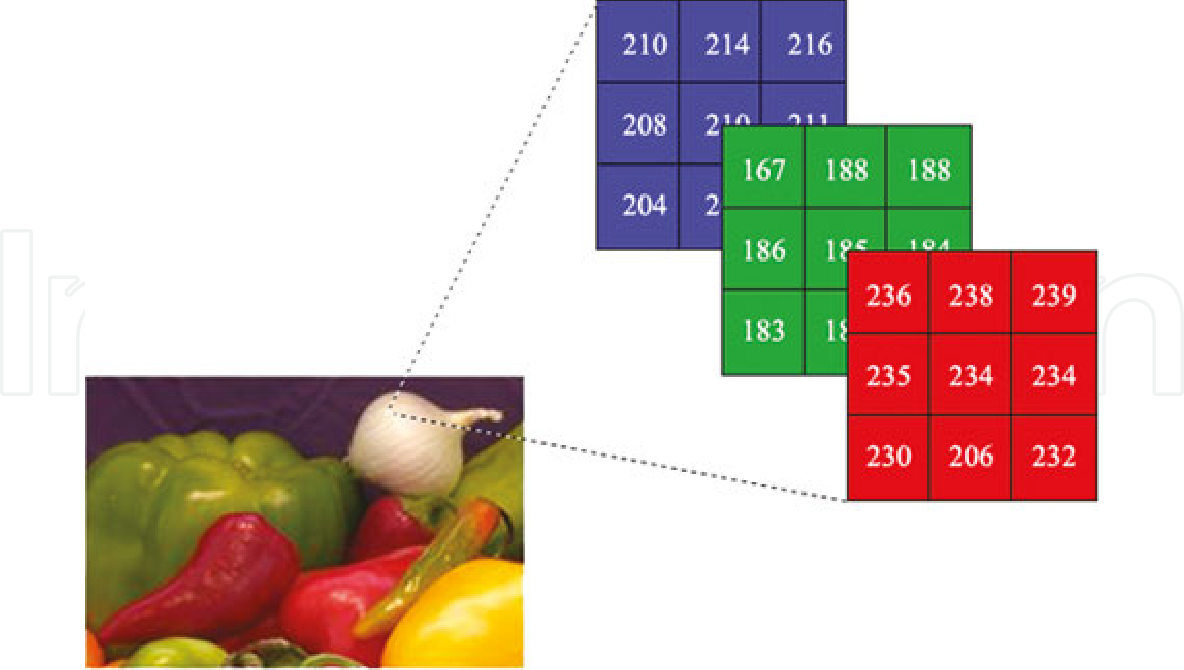
\includegraphics{index_files/mediabag/4-Figure3-1.png}

}

\caption{Source: https://doi.org/10.5772/63028}

\end{figure}%

For GIS data, multiple raster bands can be thought as vector attributes
- each band will hold the values of a specific variable (i.e.~one band
for temperature, and one for humidity). In fact, it may help to frame
rasters in terms of their vector equivalents:

\begin{longtable}[]{@{}
  >{\raggedright\arraybackslash}p{(\columnwidth - 4\tabcolsep) * \real{0.3333}}
  >{\raggedright\arraybackslash}p{(\columnwidth - 4\tabcolsep) * \real{0.3333}}
  >{\raggedright\arraybackslash}p{(\columnwidth - 4\tabcolsep) * \real{0.3333}}@{}}
\toprule\noalign{}
\begin{minipage}[b]{\linewidth}\raggedright
\end{minipage} & \begin{minipage}[b]{\linewidth}\raggedright
Vector
\end{minipage} & \begin{minipage}[b]{\linewidth}\raggedright
Raster
\end{minipage} \\
\midrule\noalign{}
\endhead
\bottomrule\noalign{}
\endlastfoot
Data variables & Vector Attributes & Raster Bands \\
Data values & Attribute values & Pixel values \\
Select ranges of data values & \texttt{Select\ by\ expression} &
\texttt{Raster\ calculator} and/or \texttt{Mask} \\
Calculate new variables & \texttt{Field\ Calculator} &
\texttt{Raster\ Calculator} \\
Calculate feature areas & \texttt{Field\ Calculator} (\texttt{\$area}) &
\texttt{Raster\ layer\ unique\ values} \\
Select by spatial location & \texttt{Select\ By\ Location} (Vec
\textgreater{} Vec) & Extract Raster Values (Points \textgreater{}
Raster) \\
& & Zonal Statistics (Polygons \textgreater{} Raster) \\
& & Zonal Statistics (Raster \textgreater{} Raster) \\
\end{longtable}

We will cover most of the above this week, and then cover how to extract
values from raster based on other layers on Week 6. For today, we will
learn how to inspect and style raster data, and also how to do some
mathematical operations among raster layers using the raster equivalent
of the \texttt{Field\ Calculator} - the \texttt{Raster\ calculator}.

\section{Before you start!}\label{before-you-start-3}

\begin{enumerate}
\def\labelenumi{\arabic{enumi}.}
\tightlist
\item
  Go through the Week 3 preparatory session on Canvas, and watch the
  seminar recording if you have missed it.
\end{enumerate}

\section{Guided Exercise 1 - Opening and inspecting raster
data}\label{guided-exercise-1---opening-and-inspecting-raster-data}

\begin{enumerate}
\def\labelenumi{(\arabic{enumi})}
\setcounter{enumi}{116}
\tightlist
\item
  For this exercise we will look at three different raster layers. The
  data has been pre-packaged and can be
  \href{https://stir-my.sharepoint.com/:u:/g/personal/ala2_stir_ac_uk/ESim8eCFo_ZCkZ4DQJ6eKpcBSJQSWHQErdPpkgcktwrXtg?e=5eG27g}{downloaded
  here}. It includes the following datasets:
\end{enumerate}

\begin{itemize}
\item
  UK SRTM: This is a single-band raster containing data from the
  {[}Shuttle Radar Topography Mission (SRTM){]}
  (https://en.wikipedia.org/wiki/Shuttle\_Radar\_Topography\_Mission), a
  global dataset of surface elevation. The data can be obtained from a
  variety of sources online.
\item
  UK Bioclim: The BIOCLIM suite of climate data has been developed to
  support biodiversity studies and species distribution modelling. It is
  a single multiband raster file.
  \href{https://www.worldclim.org/data/bioclim.html}{Read this page} for
  a description of which variable each band represents.
\item
  CORINE land cover: CORINE is a
  \href{https://land.copernicus.eu/en/products/corine-land-cover}{EU-wide
  land cover map} that is produced by the Copernicus Space Program. The
  pixel values are numerical codes that specify the different land cover
  classes. A description of each land cover number is given
  \href{https://land.copernicus.eu/content/corine-land-cover-nomenclature-guidelines/html/}{here}.
\item
  UK administrative boundaries from the \href{https://gadm.org/}{GADM
  website}, in geopackage vector file format.
\end{itemize}

\begin{enumerate}
\def\labelenumi{(\arabic{enumi})}
\setcounter{enumi}{117}
\item
  Download the required data and organise it as you have learned. Create
  a new QGIS project and add the \texttt{UK\_SRTM.tif},
  \texttt{UK\_Bioclim.tif} and
  \texttt{CLC2018\_CLC2018\_V2018\_20\_UKclip.tif} raster files to your
  project. All files are in
  \href{https://en.wikipedia.org/wiki/GeoTIFF}{\emph{GeoTIFF}'} format,
  which is the most common and standard spatial raster file format.
\item
  For each of the raster layers, right-click on the layer name and go to
  \texttt{Properties\ \textgreater{}\ Information}, then:
\end{enumerate}

\begin{tcolorbox}[enhanced jigsaw, coltitle=black, toprule=.15mm, breakable, opacitybacktitle=0.6, left=2mm, colback=white, leftrule=.75mm, rightrule=.15mm, colbacktitle=quarto-callout-important-color!10!white, toptitle=1mm, titlerule=0mm, colframe=quarto-callout-important-color-frame, arc=.35mm, bottomtitle=1mm, opacityback=0, bottomrule=.15mm, title=\textcolor{quarto-callout-important-color}{\faExclamation}\hspace{0.5em}{Stop and Think}]

\begin{enumerate}
\def\labelenumi{\alph{enumi})}
\item
  What is the \emph{data model} of these files?
\item
  What is the \emph{file format} of these files?
\item
  What are the \emph{data types} of each raster file? Why is that
  important?
\item
  What are the CRSs of each dataset you have?
\item
  What are the dimensions (rows, columns) of each raster dataset?
\item
  How many \emph{bands} does each raster dataset have?
\item
  What are the \emph{pixel sizes} (spatial resolution) of each raster
  dataset?
\end{enumerate}

\end{tcolorbox}

\begin{tcolorbox}[enhanced jigsaw, toprule=.15mm, breakable, left=2mm, colframe=quarto-callout-important-color-frame, colback=white, arc=.35mm, leftrule=.75mm, opacityback=0, rightrule=.15mm, bottomrule=.15mm]

\vspace{-3mm}\textbf{Click for answer}\vspace{3mm}

\begin{enumerate}
\def\labelenumi{\alph{enumi})}
\item
  raster (vector for the boundaries)
\item
  GeoTIFF for the rasters, geopackage for the vector
\item
  The data types can be found when looking at
  \texttt{Properties\ \textgreater{}\ Information} for a raster layer.
  The SRTM and CORINE datasets are 16-bit signed integer (INT16), the
  BIOCLIM dataset is a 32-but floating point raster. Raster data types
  are important as they determine the range and precision of the data
  that can be stored in the raster, and also impact the size of the
  raster file. For the same number of rows, columns and bands, a 32-bit
  raster is twice as large as a 16-bit raster.
\item
  GADM, SRTM, BIOCLIM: EPSG 4236 (WGS-84); CORINE: EPSG3035 (ETRS89 /
  Europe LAEA)
\item
  These are also found in
  \texttt{Properties\ \textgreater{}\ Information}, as \texttt{Width}
  (columns) and \texttt{Height}(rows) or in \texttt{Dimensions}. SRTM:
  16355 cols x 12036 rows; CORINE: 10473 cols x 12261 rows; BIOCLIM:
  1471 cols x 1084 rows.
\item
  These are also found in
  \texttt{Properties\ \textgreater{}\ Information}, as a list of bands,
  or in \texttt{Dimensions}. SRTM: 1 band, CORINE 1 band; BIOCLIM: 19
  bands.
\item
  These are also found in
  \texttt{Properties\ \textgreater{}\ Information} in
  \texttt{Pixel\ Size}. SRTM: 0.0008084837557075693617 degrees; CORINE:
  100m; BIOCLIM: 0.008983152841195215371 degrees.
\end{enumerate}

\end{tcolorbox}

\section{Guided Exercise 2 - Reprojecting raster
data}\label{guided-exercise-2---reprojecting-raster-data}

As we learned in week 1, the UK looks ``squished'' because the data is
projected using only the WGS-84 datum and geographic coordinates
(EPSG:4236). Although data in geographic coordinates is often referred
to as ``unprojected,'' this is not actually true (you are looking at it
on a flat screen, right?). For these ``unprojected'' datasets, what most
GIS software do is to simply use a linear function to convert latitudes
and longitudes in degrees to x and y values on your screen. This
projection can be referred to as Plate Carrée or Equirectangular
projection, which has a heavy amount of distortion towards the poles:

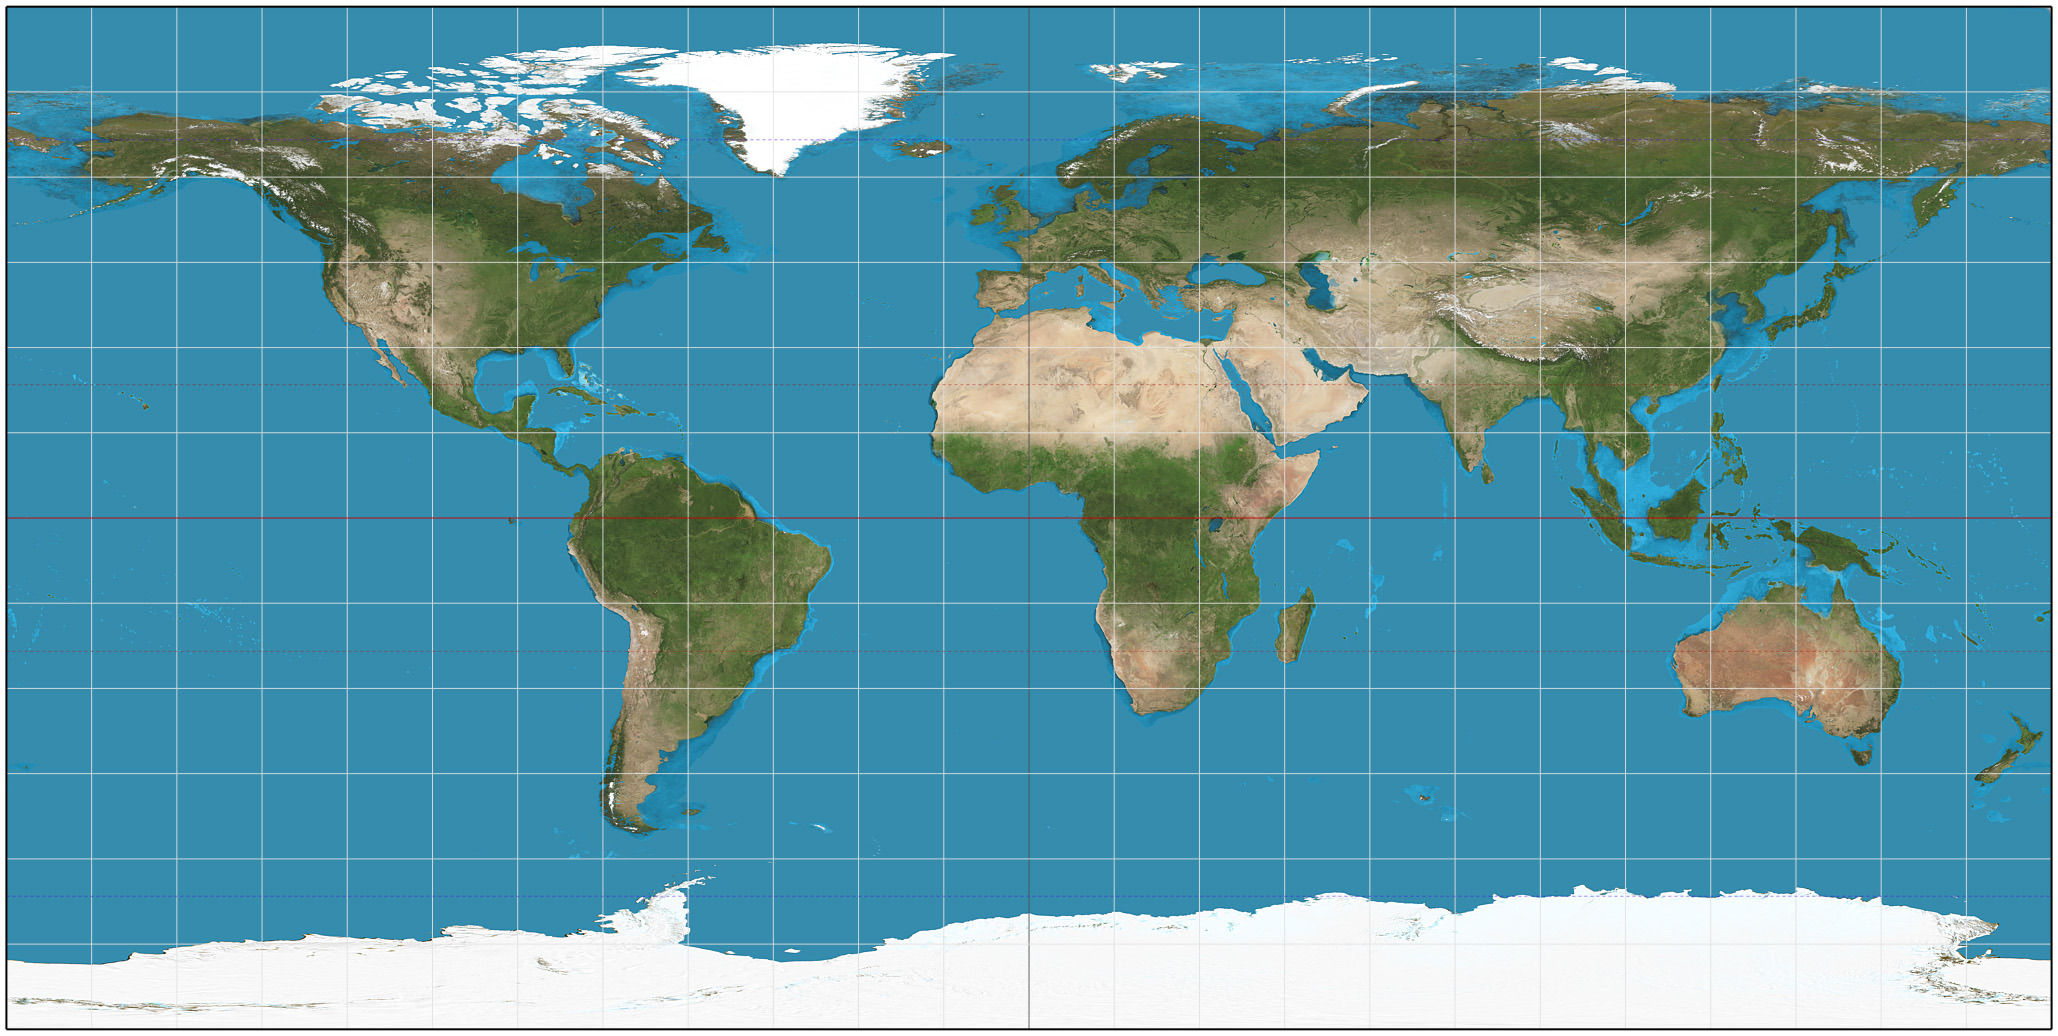
\includegraphics{images/lab_5/lab5_fig1_Equirectangular_projection_SW.jpg}

\begin{enumerate}
\def\labelenumi{(\arabic{enumi})}
\setcounter{enumi}{119}
\item
  To reproject raster data, go to
  \texttt{Raster\ \textgreater{}\ Projections\ \textgreater{}\ Warp\ (Reproject...)}.
  Select your SRTM layer as the Input Layer, and the EPSG:
  \texttt{27700\ -\ OSGB\ 1936\ /\ British\ National\ Grid} as the
  \texttt{Target\ CRS}. (If you don't see it as an option, click on the
  small button to the right to bring up the CRS selection window). Set
  the \texttt{Output\ file\ resolution...} to \texttt{90} (this will be
  in meters, as meters are the units of the BNG projection). Leave
  everything else as default. Then click on the \texttt{...} button to
  pick an appropriate folder location. Name your file
  \texttt{UK\_SRTM\_BG.tif}. \texttt{Run} the algorithm and then
  \texttt{Close} when finished.
\item
  Repeat the process for the Bioclim layer (use a cell size of 1000m)
  and the CORINE land cover map (cell size of 100m). These cell sizes
  are the meter equivalent of the degree pixel sizes the data currently
  has. Make sure you add the \texttt{\_BG} suffix to the new file names
  to keep track of what has changed from one file to the other.
\item
  If it seems nothing has really changed, remember that QGIS does
  reprojections ``on the fly'' to make sure data on the screen are all
  aligned to the project CRS. So as you learned in Week 1, change the
  project CRS to EPSG:27700 as well. Now everything should look good.
\item
  Remove the original layers from the project and keep only the
  reprojected ones, then save your project.
\end{enumerate}

\section{Guided Exercise 3 - Masking rasters using
vectors}\label{guided-exercise-3---masking-rasters-using-vectors}

We often want to remove portions (specific cells) of a raster, a process
called \emph{masking}. For example, some of our datasets include the
Republic of Ireland and bits of mainland Europe, and some datasets
include the Shetland Islands, while others don't. Let use the UK
boundaries from the GADM dataset to mask our data to the Island of Great
Britain (Scotland, England and Wales) only.

\begin{enumerate}
\def\labelenumi{(\arabic{enumi})}
\setcounter{enumi}{123}
\tightlist
\item
  First add the GADM data (\texttt{gadm36\_GBR.gpkg}) to your project.
  This geopackage holds multiple layers for the different levels of
  admin boundaries. You can just add the level 0 layer, which gets the
  UK as a whole.
\end{enumerate}

\begin{tcolorbox}[enhanced jigsaw, coltitle=black, toprule=.15mm, breakable, opacitybacktitle=0.6, left=2mm, colback=white, leftrule=.75mm, rightrule=.15mm, colbacktitle=quarto-callout-important-color!10!white, toptitle=1mm, titlerule=0mm, colframe=quarto-callout-important-color-frame, arc=.35mm, bottomtitle=1mm, opacityback=0, bottomrule=.15mm, title=\textcolor{quarto-callout-important-color}{\faExclamation}\hspace{0.5em}{Stop and Think}]

Why did you get a warning window when you added the layer to the
project?

\end{tcolorbox}

\begin{tcolorbox}[enhanced jigsaw, toprule=.15mm, breakable, left=2mm, colframe=quarto-callout-important-color-frame, colback=white, arc=.35mm, leftrule=.75mm, opacityback=0, rightrule=.15mm, bottomrule=.15mm]

\vspace{-3mm}\textbf{Click for answer}\vspace{3mm}

Because this layer has a different CRS than the project, and QGIS it is
asking you how to deal with it.

\end{tcolorbox}

\begin{enumerate}
\def\labelenumi{(\arabic{enumi})}
\setcounter{enumi}{124}
\tightlist
\item
  As we learned on Week 1, trying to do clipping (and masking)
  operations between layers with mismatched CRSs gives us wrong results.
  So before you do anything, reproject the UK boundaries layer to EPSG
  27700. \textbf{DO NOT} go to
  \texttt{Properties\ \textgreater{}\ Layer\ CRS} - that won't reproject
  the data, just force a new CRS definition on it without changing the
  actual coordinates, and you will ruin your data. Go to
  \texttt{Vector\ \textgreater{}\ Data\ Management\ Tools\ \textgreater{}\ Reproject\ Layer}.
\end{enumerate}

You also need to extract the \textbf{mainland} British Island from the
rest of the dataset (just the one polygon that represents the bigger
land mass). Turns out there is a quick way to do both at once, but first
we need to deal with a little issue with the vector layer:

\begin{enumerate}
\def\labelenumi{(\arabic{enumi})}
\setcounter{enumi}{125}
\tightlist
\item
  Open the Attribute Table of the UK boundaries layer. How many features
  does it have?
\end{enumerate}

This is what is called a \texttt{multipart} polygon - a set of disjoint
polygons all treated as a single feature. Before we can use the layer,
we need to split the individual polygons apart to be able to select the
main island only:

\begin{enumerate}
\def\labelenumi{(\arabic{enumi})}
\setcounter{enumi}{126}
\item
  Go to
  \texttt{Vector\ \textgreater{}\ Geometry\ Tools\ \textgreater{}\ Multipart\ to\ Singleparts},
  and select the GADM layer. You can leave it as a temporary layer since
  we will only export one polygon for it in the next step. A new temp
  layer called \texttt{Single\ parts} will be created. Inspect its
  Attribute Table.
\item
  Now use the feature selection tool
  (
\includegraphics{index_files/mediabag/mActionSelectRectang.png}) to
  select the one polygon for the mainland Great Britain only (no smaller
  islands!), and then right-click on the Single Part layer name and
  choose
  \texttt{Export\ \textgreater{}\ Save\ selected\ features\ as...}. Pick
  a folder location and name the file \texttt{GB\_Island.shp}. Before
  you click on OK, however, change the \texttt{CRS} drop-down menu to
  EPSG:27700. That is it, QGIS will now reproject the layer before
  saving it! Click \texttt{OK}to save, and then remove the original GADM
  and the temp layer from your project to keep things tidy. Save your
  project.
\item
  Double check what is the CRS of the new \texttt{GB\_island} layer you
  have created.
\item
  You are now ready to mask the raster data. Go to
  \texttt{Raster\ \textgreater{}\ Extraction\ \textgreater{}\ Clip\ Raster\ by\ Mask\ Layer...}.
  As \texttt{Input\ layer}, select the SRTM layer, and as
  \texttt{Mask\ layer}, select the GB island layer. Then on the option
  \texttt{Assign\ a\ specific\ nodata\ value\ to\ output\ bands}, enter
  the number \texttt{-32768}. \emph{Make sure you include the minus
  sign}! Leave the other options as default but do check both the
  \texttt{Match\ the\ extent\ of\ the\ clipped\ raster\ to\ the\ extent\ of\ the\ mask\ layer}
  and \texttt{Keep\ resolution\ of\ input\ raster} options. Pick a
  folder and name your file \texttt{UK\_SRTM\_BG\_GBmask.tif}. Now we
  can know at a glance that this is the SRTM data, reprojected to
  British Grid and masked to Great Britain.
\end{enumerate}

\begin{tcolorbox}[enhanced jigsaw, coltitle=black, toprule=.15mm, breakable, opacitybacktitle=0.6, left=2mm, colback=white, leftrule=.75mm, rightrule=.15mm, colbacktitle=quarto-callout-important-color!10!white, toptitle=1mm, titlerule=0mm, colframe=quarto-callout-important-color-frame, arc=.35mm, bottomtitle=1mm, opacityback=0, bottomrule=.15mm, title=\textcolor{quarto-callout-important-color}{\faExclamation}\hspace{0.5em}{Stop and Think}]

\begin{enumerate}
\def\labelenumi{\alph{enumi})}
\item
  Why did we pick a value of -32768 for `nodata'?
\item
  Why should we check the \texttt{Match\ the\ extent...} and
  \texttt{Keep\ Resolution..} boxes?
\end{enumerate}

\end{tcolorbox}

\begin{tcolorbox}[enhanced jigsaw, toprule=.15mm, breakable, left=2mm, colframe=quarto-callout-important-color-frame, colback=white, arc=.35mm, leftrule=.75mm, opacityback=0, rightrule=.15mm, bottomrule=.15mm]

\vspace{-3mm}\textbf{Click for answer}\vspace{3mm}

\begin{enumerate}
\def\labelenumi{\alph{enumi})}
\item
  Since raster layers are grids (matrices) they must always be
  rectangular in shape. So when masking a raster using an irregular
  shape, the pixels outside the polygon will receive a value indicating
  \emph{nodata}, but they will still exist. The default nodata value for
  QGIS is zero, but since we are dealing with elevations, zero is still
  a valid elevation value, and we could even have areas inland that are
  at sea level or lower, and thus have an elevation of zero or below. We
  also know our data is a signed 16-bit integer, that can take values
  from -32,768 to +32,767. So we pick the most negative elevation number
  within this range, which also would never occur on land (-32768
  meters) to use as nodata.
\item
  By selecting the
  \texttt{Match\ the\ extent\ of\ the\ clipped\ raster\ to\ the\ extent\ of\ the\ mask\ layer}
  option when masking, the extent of the raster rectangle will be just
  enough to cover the GB polygon. If we left that unchecked, QGIS would
  set the non GB pixels to `nodata', but leave the raster with the
  original dimensions. That would be a waste of disk space. We also
  check \texttt{Keep\ resolution...} to make sure QGIS doesn;t change
  the pixel sizes to better `fit' the rectangle to the extent. The
  spatial resolution of a raster file often has a reason to be, and we
  don't want to arbitrarily change that.
\end{enumerate}

\end{tcolorbox}

\begin{enumerate}
\def\labelenumi{(\arabic{enumi})}
\setcounter{enumi}{130}
\item
  Use the \texttt{Identify\ Features} tool
  (
\includegraphics{index_files/mediabag/mActionIdentify.png}) to click
  on blank area of the masked SRTM layer (near the shore). Make sure you
  have the SRTM layer selected on the Layers panel before you click the
  tool. What pixel values do you get? -32768 or `nodata'?
\item
  Now go to the \texttt{Properties\ \textgreater{}\ Transparency} tab of
  the SRTM raster layer, and uncheck the
  \texttt{No\ data\ value:\ -32768} box. Look at your raster again, and
  probe the same areas with the \texttt{Identify\ Features} tool. Can
  you see now how the actual raster is still a rectangle, with the
  pixels outside the mask set to -32768? Before you proceed, go back and
  check the \texttt{No\ data:\ -32768} box again.
\item
  Now repeat the masking for the CORINE and BIOCLIM layers. You can use
  the same nodata number for the CORINE and BIOCLIM layers. The CORINE
  layer actually already has nodata defined as \texttt{-32768} so we
  just keep it. And for Bioclim, it is an unlikely value for any of the
  climatic variables, and because the climate data is a floating-point
  number (decimal), it is almost impossible that a perfect value of
  -32768.000000 would exist in the data naturally.
\item
  Remove the non-masked raster datasets from your project and save it.
\item
  Now zoom in into any place on the coastline, and answer:
\end{enumerate}

\begin{tcolorbox}[enhanced jigsaw, coltitle=black, toprule=.15mm, breakable, opacitybacktitle=0.6, left=2mm, colback=white, leftrule=.75mm, rightrule=.15mm, colbacktitle=quarto-callout-important-color!10!white, toptitle=1mm, titlerule=0mm, colframe=quarto-callout-important-color-frame, arc=.35mm, bottomtitle=1mm, opacityback=0, bottomrule=.15mm, title=\textcolor{quarto-callout-important-color}{\faExclamation}\hspace{0.5em}{Stop and Think}]

Why don't the edges of each raster dataset line up perfectly?

\end{tcolorbox}

\begin{tcolorbox}[enhanced jigsaw, toprule=.15mm, breakable, left=2mm, colframe=quarto-callout-important-color-frame, colback=white, arc=.35mm, leftrule=.75mm, opacityback=0, rightrule=.15mm, bottomrule=.15mm]

\vspace{-3mm}\textbf{Click for answer}\vspace{3mm}

\begin{enumerate}
\def\labelenumi{\alph{enumi})}
\tightlist
\item
  Again, this is a side effect from raster layers being grids. As each
  one has a different pixel size, the \texttt{decision} of which pixel
  is inside or outside the GB vector polygon will be different for each
  layer. Also, the coastline will always appear `ragged' because we
  can't represent any detail smaller than a single pixel on a raster
  file - and the pixel grids of the three layers do not align because of
  the pixel sizes.
\end{enumerate}

\end{tcolorbox}

\section{Guided Exercise 4 - Styling raster
data}\label{guided-exercise-4---styling-raster-data}

Just as with vector data, QGIS offers many options for the symbology of
raster data. You will see some similarities between the symbology
options for vectors and rasters, but also some differences because of
the nature of each data model.

\begin{enumerate}
\def\labelenumi{(\arabic{enumi})}
\setcounter{enumi}{135}
\tightlist
\item
  Turn off all layers except the CORINE land cover, and then go to its
  \texttt{Properties\ \textgreater{}\ Symbology}. Note that the default
  \texttt{Render\ Type} for single-band rasters is
  \texttt{Singleband\ gray}. That means pixels are coloured by a shade
  of grey that is proportional to its numeric value, with higher values
  being closer to white. Change it to
  \texttt{Paletted\ /\ Unique\ Values}. Maintain the \texttt{Band\ 1}
  selection (there is only one band anyway) and \texttt{Random\ Colors}
  options, and then click on \texttt{Classify}. Apply the result to your
  raster and visualise it.
\end{enumerate}

\begin{tcolorbox}[enhanced jigsaw, coltitle=black, toprule=.15mm, breakable, opacitybacktitle=0.6, left=2mm, colback=white, leftrule=.75mm, rightrule=.15mm, colbacktitle=quarto-callout-important-color!10!white, toptitle=1mm, titlerule=0mm, colframe=quarto-callout-important-color-frame, arc=.35mm, bottomtitle=1mm, opacityback=0, bottomrule=.15mm, title=\textcolor{quarto-callout-important-color}{\faExclamation}\hspace{0.5em}{Stop and Think}]

\begin{enumerate}
\def\labelenumi{\alph{enumi})}
\item
  How many categories are there on this raster?
\item
  What are the pixel values representing?
\item
  What would be the vector symbology equivalent of
  \texttt{Paletted\ /\ Unique\ Values}?
\end{enumerate}

\end{tcolorbox}

\begin{tcolorbox}[enhanced jigsaw, toprule=.15mm, breakable, left=2mm, colframe=quarto-callout-important-color-frame, colback=white, arc=.35mm, leftrule=.75mm, opacityback=0, rightrule=.15mm, bottomrule=.15mm]

\vspace{-3mm}\textbf{Click for answer}\vspace{3mm}

\begin{enumerate}
\def\labelenumi{\alph{enumi})}
\item
  36 categories (unique pixel values)
\item
  Each pixel value is a numerical code that indicates a land cover type.
\item
  the \texttt{Categorized} option.
\end{enumerate}

\end{tcolorbox}

Whoa, there are a lot of classes, and the random colours selection
picked colours that are very similar to one another for some of the
classes. Fortunately for us, the data producers of CORINE include a
colour map file as part of the metadata. Let us use it!

\begin{enumerate}
\def\labelenumi{(\arabic{enumi})}
\setcounter{enumi}{136}
\item
  Back on the \texttt{Properties\ \textgreater{}\ Symbology} window,
  click on the \texttt{...} button to the right of \texttt{Delete\ All}
  and choose \texttt{Load\ Color\ Map\ from\ File...}. Within the CORINE
  files you unzipped, find and select the metadata file named
  \texttt{CLC2018\_CLC2018\_V2018\_20\_QGIS.txt}. \texttt{Apply}and then
  click \texttt{OK}. Not only we get the colours selected by the CORINE
  mapping team, but also all the proper class names! That was nice!
\item
  Now let us have a look at the BIOCLIM dataset. First, read the
  metadata included with the data files (\texttt{Bioclim\_metadata.txt})
  to understand what each band of this dataset represents. Then turn on
  the BIOLCIM layer and turn the remaining layers off.
\end{enumerate}

\begin{tcolorbox}[enhanced jigsaw, coltitle=black, toprule=.15mm, breakable, opacitybacktitle=0.6, left=2mm, colback=white, leftrule=.75mm, rightrule=.15mm, colbacktitle=quarto-callout-important-color!10!white, toptitle=1mm, titlerule=0mm, colframe=quarto-callout-important-color-frame, arc=.35mm, bottomtitle=1mm, opacityback=0, bottomrule=.15mm, title=\textcolor{quarto-callout-important-color}{\faExclamation}\hspace{0.5em}{Stop and Think}]

Why does the BIOCLIM layer appears to be coloured?

\end{tcolorbox}

\begin{tcolorbox}[enhanced jigsaw, toprule=.15mm, breakable, left=2mm, colframe=quarto-callout-important-color-frame, colback=white, arc=.35mm, leftrule=.75mm, opacityback=0, rightrule=.15mm, bottomrule=.15mm]

\vspace{-3mm}\textbf{Click for answer}\vspace{3mm}

When QGIS opens a multiband, single file raster, it always thinks that
the file is an image, and thus it automatically assigns the first three
bands of the file to the Red, Green, and Blue colour channels. We will
look at raster images in the next session, but this colour composition
clearly doesn't make sense for our climate data, so let us change it.

\end{tcolorbox}

\begin{enumerate}
\def\labelenumi{(\arabic{enumi})}
\setcounter{enumi}{138}
\tightlist
\item
  Go to the \texttt{Properties\ \textgreater{}\ \ Symbology} window for
  the BIOCLIM dataset. Notice the default symbology choice of
  \texttt{Multiband\ color}. Since each band of our data represents a
  different climatic variable, with continuous numeric values (not
  categories or classes), we need to pick the
  \texttt{Single\ band\ -\ pseudocolor} option. Choose the \texttt{bio1}
  band, and for the colour ramp, click on the down-arrow button to the
  right of the colour palette button, and select the \texttt{magma}
  colour ramp. Classify the existing values and then \texttt{Apply} and
  click \texttt{OK}. What does the layer look like now?
\end{enumerate}

\begin{tcolorbox}[enhanced jigsaw, coltitle=black, toprule=.15mm, breakable, opacitybacktitle=0.6, left=2mm, colback=white, leftrule=.75mm, rightrule=.15mm, colbacktitle=quarto-callout-important-color!10!white, toptitle=1mm, titlerule=0mm, colframe=quarto-callout-important-color-frame, arc=.35mm, bottomtitle=1mm, opacityback=0, bottomrule=.15mm, title=\textcolor{quarto-callout-important-color}{\faExclamation}\hspace{0.5em}{Stop and Think}]

\begin{enumerate}
\def\labelenumi{\alph{enumi})}
\item
  What would be the vector symbology equivalent of
  \texttt{Single\ band\ \ -\ pseudocolor}?
\item
  What climatic variable is ``bio01'' representing?
\item
  What units are the minimum and maximum values shown on the colour
  scale?
\item
  Why such a strange choice for the units?
\end{enumerate}

\end{tcolorbox}

\begin{tcolorbox}[enhanced jigsaw, toprule=.15mm, breakable, left=2mm, colframe=quarto-callout-important-color-frame, colback=white, arc=.35mm, leftrule=.75mm, opacityback=0, rightrule=.15mm, bottomrule=.15mm]

\vspace{-3mm}\textbf{Click for answer}\vspace{3mm}

\begin{enumerate}
\def\labelenumi{\alph{enumi})}
\item
  The \texttt{Graduated} option.
\item
  The metadata file tells us it is Annual Mean Temperature.
\item
  The metadata file also tells us it is °C * 10 (degrees Celsius times
  ten)
\item
  This is an old \texttt{trick} to reduce file sizes while keeping some
  precision. Let's say the data creators wanted to record temperatures
  with one decimal place of precision. If they stored the data as a
  floating point, we would need 32-bit files. But if we consider that
  mean annual temperatures on Earth will easily be contained in the
  range of -100 to +100 degrees Celsius, we could instead multiply all
  numbers by ten, and store them as 16-bit integers instead, cutting
  file sizes in half. For example, a temperature of 32.7°C becomes a
  pixel value of 327.
\end{enumerate}

\end{tcolorbox}

\begin{enumerate}
\def\labelenumi{(\arabic{enumi})}
\setcounter{enumi}{139}
\tightlist
\item
  Explore some of the other climatic variables contained in the BIOCLIM
  dataset, using different colour ramps.
\end{enumerate}

Finally, let's work on the symbology for the SRTM data. For that, we
will take advantage of some nice scientific colour palettes that are
built-in on QGIS. We will talk about what makes these palettes special
on Week 4 but let us just use them now.

\begin{enumerate}
\def\labelenumi{(\arabic{enumi})}
\setcounter{enumi}{140}
\item
  On the \texttt{Properties\ \textgreater{}\ Symbology} window of the
  SRTM layer, choose the \texttt{Singleband\ Pseudocolor} option, and
  then on the down arrow button besides the \texttt{Color\ Ramp} option,
  select \texttt{Create\ New\ Color\ Ramp}. On the small options window
  that comes up, select \texttt{Catalog:cpt-city}.
\item
  Once the catalogue window opens, go to the \texttt{Topography} list
  and select the \texttt{cd-a} palette. Then manually enter \texttt{Min}
  and \texttt{Max} values, using \texttt{0} and \texttt{900}
  respectively. \texttt{Apply} and see how it changes. But before
  clicking on \texttt{OK}, go to the \texttt{Transparency} tab and drag
  the slider at the top to around \texttt{60\%}. That will let other
  layers under it to show through and blend with the colours.
\item
  Right-click on the SRTM layer name and select
  \texttt{Duplicate\ layer}. This option creates a `virtual' copy of the
  layer - it will still point to the same file on disk, but you are able
  to select a different symbology for it.
\end{enumerate}

(@)Now, on the \texttt{Properties\ \textgreater{}\ Symbology} of the
copied layer, change the render type to \texttt{Hillshade}. Leave
everything as default, then \texttt{Apply} and close the window. Make
sure both the coloured and the hillshade SRTM layers are turned on in
the Layer Panel, and that the hillshade layer is immediately under the
coloured SRTM layer. Zoom in and turn each layer on and off in turn to
understand how this neat `3-D' visual effect works.

\begin{tcolorbox}[enhanced jigsaw, coltitle=black, toprule=.15mm, breakable, opacitybacktitle=0.6, left=2mm, colback=white, leftrule=.75mm, rightrule=.15mm, colbacktitle=quarto-callout-important-color!10!white, toptitle=1mm, titlerule=0mm, colframe=quarto-callout-important-color-frame, arc=.35mm, bottomtitle=1mm, opacityback=0, bottomrule=.15mm, title=\textcolor{quarto-callout-important-color}{\faExclamation}\hspace{0.5em}{Stop and Think}]

What does the \texttt{hillshade} render style does?

\end{tcolorbox}

\begin{tcolorbox}[enhanced jigsaw, toprule=.15mm, breakable, left=2mm, colframe=quarto-callout-important-color-frame, colback=white, arc=.35mm, leftrule=.75mm, opacityback=0, rightrule=.15mm, bottomrule=.15mm]

\vspace{-3mm}\textbf{Click for answer}\vspace{3mm}

It uses the elevation information to simulate how different areas of the
terrain would be illuminated or shaded by sunlight coming from a certain
sun elevation and azimuth (direction).

\end{tcolorbox}

\section{Guided Exercise 5 - Terrain
Calculations}\label{guided-exercise-5---terrain-calculations}

One of the most common raster datasets used in GIS are Digital Elevation
Models or DEMS. The structure of raster data is particularly well suited
to represent terrain, in its continuous and highly variable nature.
Moreover, terrain and elevation data is often a key variable in GIS
analysis, as it directly influences most biological, geological and
anthropic processes.

For this reason, a few specific terrain analysis tools that are always
included in GIS software, and used often. These are the methods to
calculate
\href{https://en.wikipedia.org/wiki/Grade_(slope)}{slopes}(a.k.a grades,
gradients),
\href{https://en.wikipedia.org/wiki/Aspect_(geography)}{aspects} and
\href{https://en.wikipedia.org/wiki/Viewshed}{viewsheds}, using DEMs as
the base data.

\subsection{Plugins}\label{plugins}

In this exercise, you will also learn about one of the most powerful
aspects of QGIS: \emph{plugins}. As you may know, QGIS is a free and
open-source software, meaning anyone can contribute to the code. QGIS
also makes it easy for its functionality to be extended via plugins,
separate little `apps' that add new tools and capabilities to the main
QGIS app. For this exercise, we will install and use two official QGIS
plugins, the \texttt{QuickMapServices} and
\texttt{Visibility\ Analysis}.

\begin{enumerate}
\def\labelenumi{(\arabic{enumi})}
\setcounter{enumi}{143}
\tightlist
\item
  Head to the menu
  \texttt{Plugins\ \textgreater{}\ Manage\ and\ Install\ Plugins}. You
  will see a window like the one below. Then select the
  \texttt{Not\ Installed} tab, and then on the search bar search for
  \texttt{QuickMapServices}. Select it on the left panel, and then click
  on \texttt{Install\ Plugin}. Then repeat this process to find and
  install the \texttt{Visibility\ Analysis} plugin.
\end{enumerate}

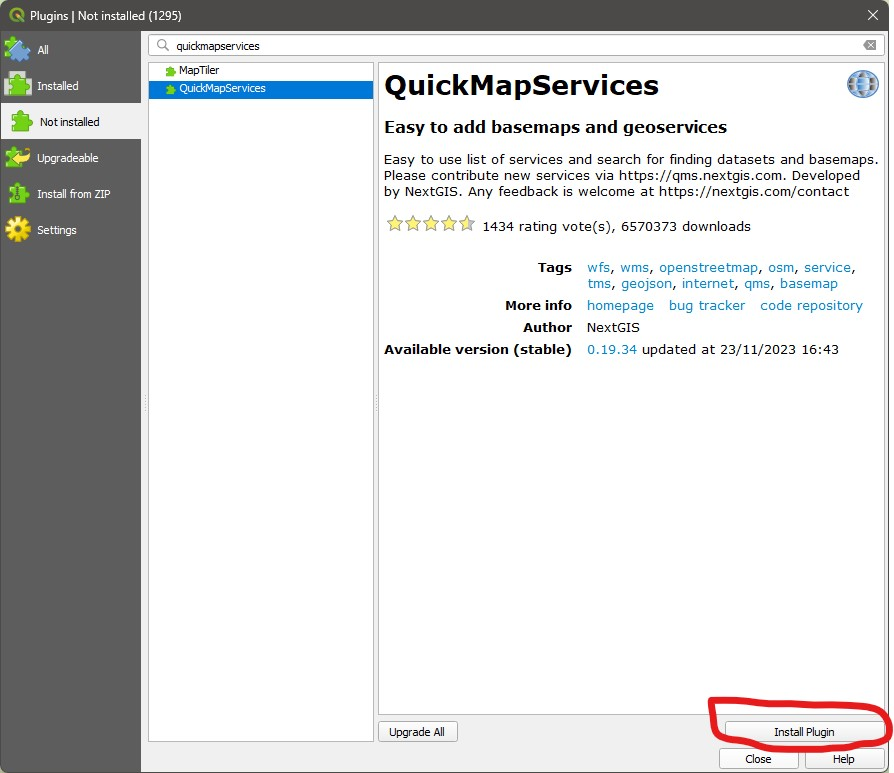
\includegraphics{images/lab_5/lab5_fig2_quickmap.jpg}

\begin{enumerate}
\def\labelenumi{(\arabic{enumi})}
\setcounter{enumi}{144}
\tightlist
\item
  The \texttt{QuickMapServices} plugin will add a new menu entry:
  \texttt{Web\ \textgreater{}\ QuickMapServices}. Once you click on it,
  you will see a list of web map services - but there is more. Go to
  \texttt{Web\ \textgreater{}\ QuickMapServices\ \textgreater{}\ Settings},
  and then click on the \texttt{More\ services} tab. Read the warning
  and click on \texttt{Get\ contributed\ pack}, and once you get a
  confirmation message, click on \texttt{Save} and exit the window.
\end{enumerate}

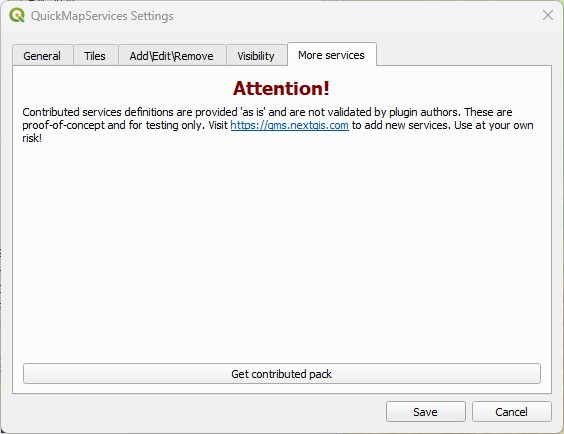
\includegraphics{images/lab_5/lab5_fig3_moremaps.jpg}

\begin{enumerate}
\def\labelenumi{(\arabic{enumi})}
\setcounter{enumi}{145}
\item
  Now go back to
  \texttt{Web\ \textgreater{}\ QuickMapServices\ \textgreater{}\ Settings},
  and you will see a list of providers. For example, go to the
  \texttt{Web\ \textgreater{}\ QuickMapServices\ \textgreater{}\ Google}
  option and add the \texttt{Google\ Hybrid} dataset directly as layer
  in your project! These layers will require you to be connected to
  Internet to work, and they won't give you many symbology options, but
  they are very handy to help in navigation when working on a project.
\item
  Take some time to explore the layers available in this plugin.
\end{enumerate}

\subsection{Masking by area}\label{masking-by-area}

Earlier today you have learned how to use a vector polygon to mask a
raster layer. But sometimes we just want to `freeform' cut a piece of a
raster, without the need to be too precise. In that case, we can use the
\texttt{Clip\ Raster\ by\ Extent} function.

\begin{enumerate}
\def\labelenumi{(\arabic{enumi})}
\setcounter{enumi}{147}
\tightlist
\item
  Make sure you \texttt{Google\ Hybrid} web layer is visible, and
  navigate until you frame the `Stirling-Glasgow-Edinburgh triangle' in
  your canvas, like the image below:
\end{enumerate}

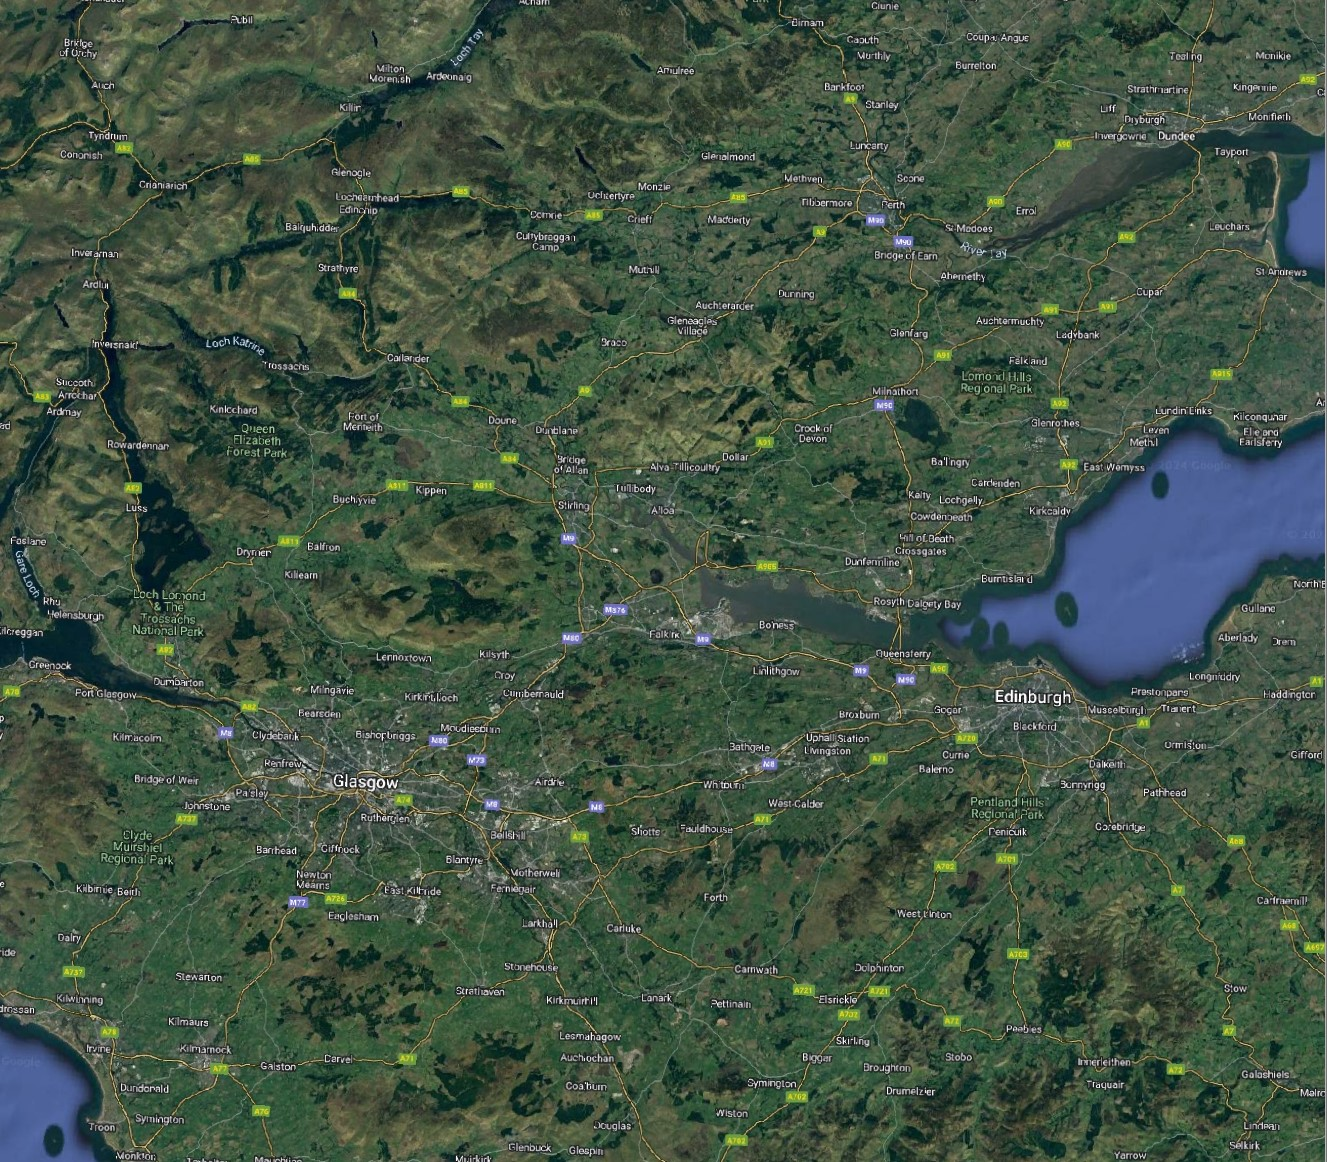
\includegraphics{images/lab_5/lab5_fig4_stirglaedi.jpg} (@) Then go to
\texttt{Raster\ \textgreater{}\ Extract\ \textgreater{}\ Clip\ Raster\ by\ Extent...}.
Pick the SRTM layer as \texttt{Input\ layer}, and then for
\texttt{Clipping\ Extent}, click on the small button to the right with a
small arrow figure. That will set the \texttt{cut\ area} to be exactly
what you are viewing on the canvas. But there are other options. If you
click on the small down-arrow button to the right, you can use the
extent (bounding box) of another layer, as well some more advanced
options. You can also click on \texttt{Draw\ on\ map\ canvas} to be
allowed to drag a rectangle over your map canvas that sets the extent of
the cut.

\begin{enumerate}
\def\labelenumi{(\arabic{enumi})}
\setcounter{enumi}{148}
\tightlist
\item
  Mask the SRTM layer to the region including Stirling, Glasgow and
  Edinburgh, either by setting you map canvas zoom and using it as
  extent, or by clicking and dragging to set the extent. Then pick a
  proper folder and save it as
  \texttt{UK\_SRTM\_BG\_centralscotland.tif}. You should end up with
  something like this (but your extent will likely vary):
\end{enumerate}

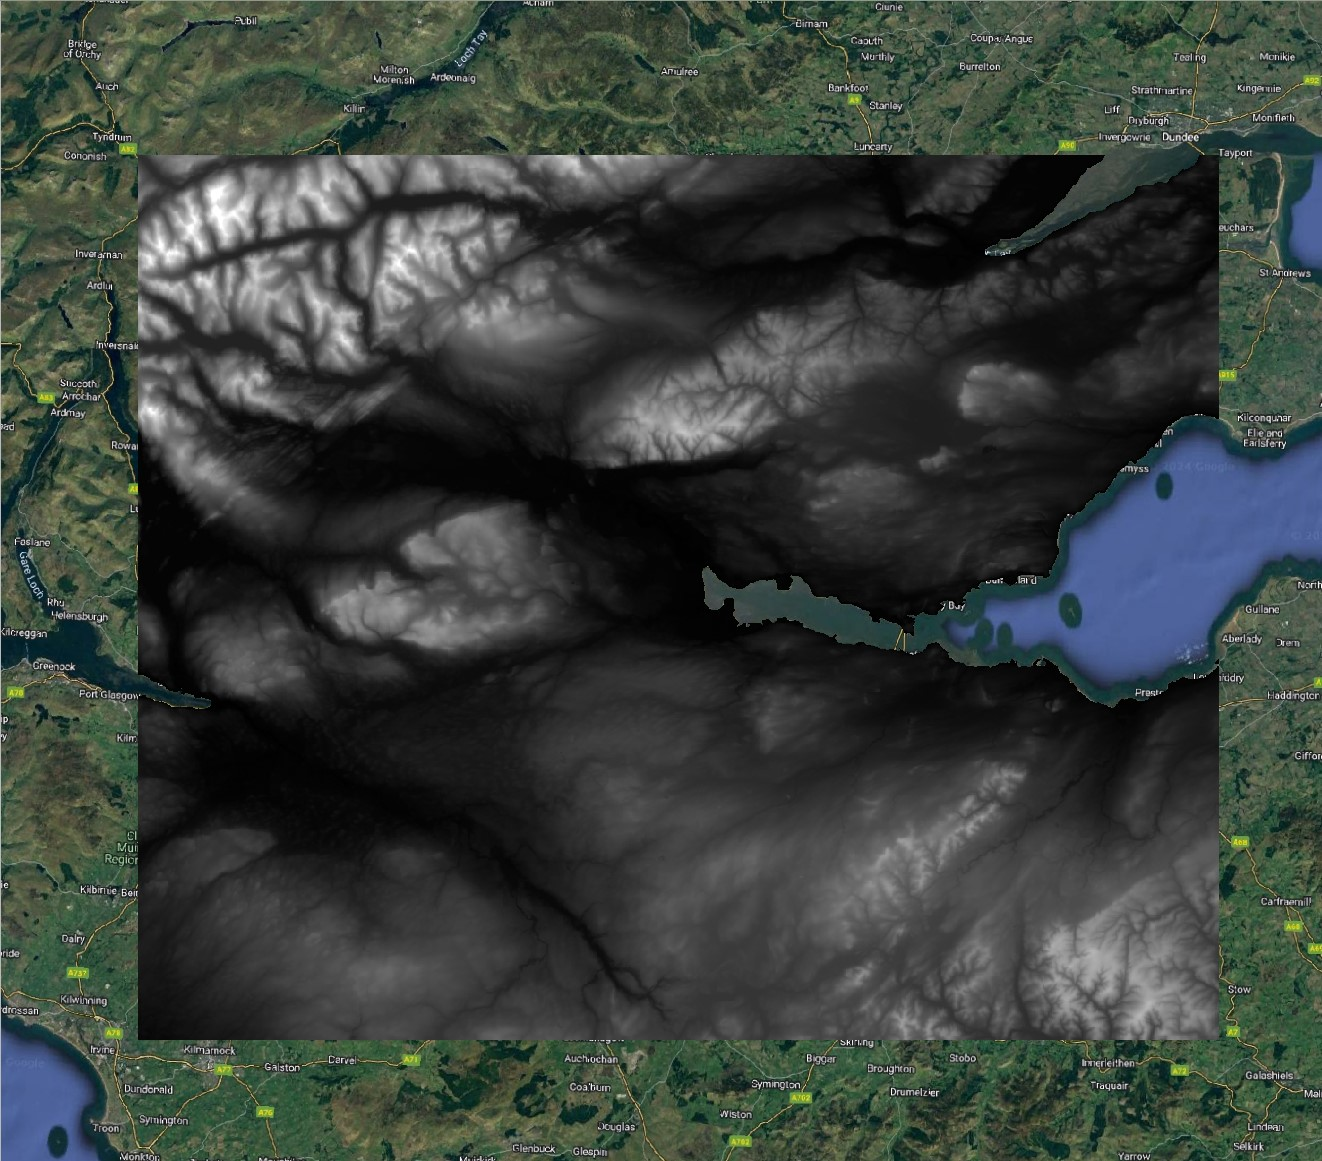
\includegraphics{images/lab_5/lab5_fig5_centralscot.jpg}

\subsection{Calculating slope and
aspect}\label{calculating-slope-and-aspect}

We can now use our Central Scotland subset to demonstrate how to
calculate slope and aspect.

\begin{enumerate}
\def\labelenumi{(\arabic{enumi})}
\setcounter{enumi}{149}
\tightlist
\item
  Go to
  \texttt{Raster\ \textgreater{}\ Analysis\ \textgreater{}\ Slope...},
  and pick the Central Scotland DEM you created as
  \texttt{Input\ Layer}. Leave everything else as default and then pick
  a proper folder to save the new file as
  \texttt{UK\_SRTM\_BG\_centralscot\_slope.tif}. Then \texttt{Run} and
  \texttt{Close}. You will get a new raster layer, where the pixel
  values indicate the steepness of each pixel, in degrees. Steep slopes
  will appear as light grey/white, and flat areas will appear dark:
\end{enumerate}

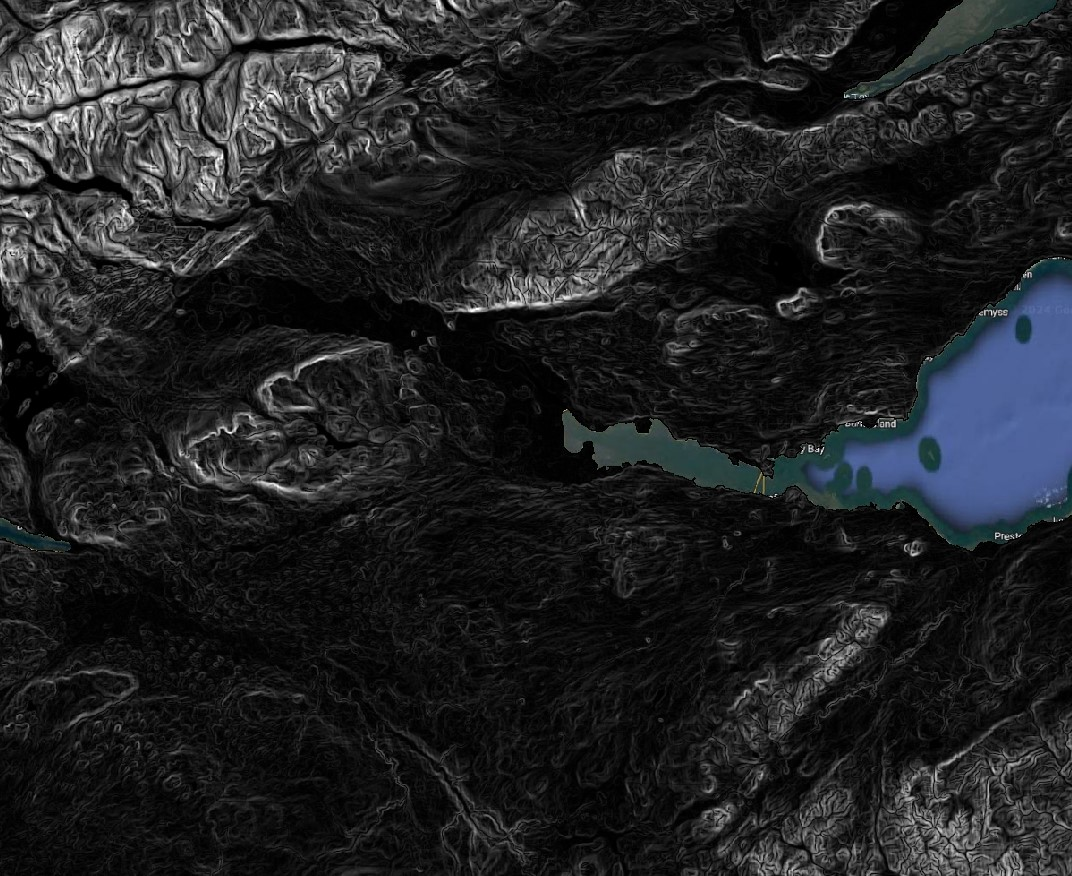
\includegraphics{images/lab_5/lab5_fig6_slope.jpg}

\begin{enumerate}
\def\labelenumi{(\arabic{enumi})}
\setcounter{enumi}{150}
\item
  Now go to
  \texttt{Raster\ \textgreater{}\ Analysis\ \textgreater{}\ Aspect...},
  and again pick the Central Scotland DEM you created as
  \texttt{Input\ Layer}. Leave everything else as default and pick a
  folder to save the new file as
  \texttt{UK\_SRTM\_BG\_centralscot\_aspect.tif}. \texttt{Run} and
  \texttt{Close}. This layer will now tell you the cardinal direction,
  in degrees (North = 0/360),, that each slope is facing.
\item
  Use the \texttt{Identify\ Features...} tool to explore some of the
  aspect and slope values you have calculated.
\end{enumerate}

\subsection{Viewshed analysis}\label{viewshed-analysis}

Finally, let us calculate a `viewshed' - a raster indicating which
points on the Earth's surface are visible from a given point,
considering the topography. Viewshed analysis is often used for
landscape planning - for example, determining from where a wind power
turbine may be visible or not.

The \texttt{Visibility\ Analysis} plugin adds some option to the
\texttt{Processing\ panel} of QGIS. To see it, click on the
\texttt{Processing\ Toolbox} button on the main QGIS toolbar
(
\includegraphics{index_files/mediabag/processingAlgorithm.png}), and
the panel will open to the right. This panel houses many, many more GIS
functions beyond those available on the \texttt{Vector} and
\texttt{Raster} menus, and we will use it often during the last weeks of
the module.

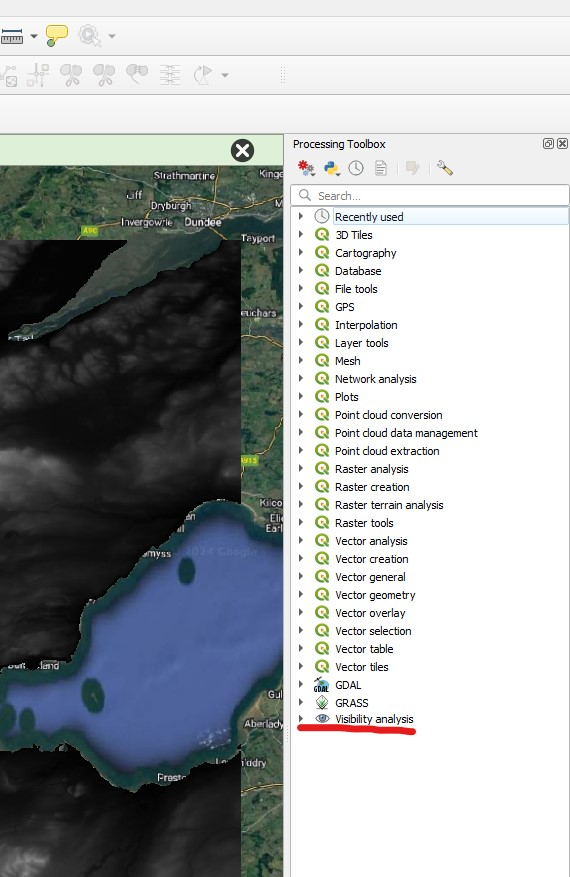
\includegraphics{images/lab_5/lab5_fig7_proc.jpg}

\begin{enumerate}
\def\labelenumi{(\arabic{enumi})}
\setcounter{enumi}{152}
\item
  Download the \texttt{observation\_point,shp}
  \href{https://stir-my.sharepoint.com/:u:/g/personal/ala2_stir_ac_uk/EWG4zHZtEchMnkRo4Dyg-0ABn8kz7vnY4MABGkHJtBn8xg?e=zMQBZu}{file
  from this link}.
\item
  Open the \texttt{Visibility\ Analysis} heading on the
  \texttt{Processing\ Toolbox}, and then double click on
  \texttt{Create\ Viewpoints}. A new window will open. On this window,
  you need to pick the \texttt{Observer\ Location}, which will be the
  Observation point layer, and then the DEM, which will be the Central
  Scotland SRTM (make sure you \emph{don't} pick the slope or aspect
  layers by mistake!).
\item
  There are many options that you don't need to worry about for now, but
  three warrant some explanation: \texttt{Radius\ of\ Analysis}
  specifies how far you want to calculate the viewshed - it is an
  expensive computation so it may make sense to limit it. Let's use
  20,000 meters for our analysis. Then pay attention to
  \texttt{Observer\ Height} and \texttt{Target\ Height}. They determine
  what is the height of the observation being made (above the elevation
  of the observation point), and what the height of the target would be.
  So again, if you are wondering if a wind power turbine would be
  visible from that location, you should add the height of the turbine
  to the \texttt{Target\ Height} field. You can leave these options at
  1.6m and zero, respectively. Then pick a folder and save the viewpoint
  as \texttt{viewpoint.shp}, and \texttt{Run} the tool.
\item
  Now go back to the \texttt{Processing\ Toolbox} and double click on
  \texttt{Viewshed}. Pick the \texttt{Viewpoint} layer as
  \texttt{Observer\ Location}, and the Central Scotland DEM as
  \texttt{Digital\ Elevation\ Model}. Leave everything else as default,
  and pick a folder to save your viewshed analysis as
  \texttt{viewshed.tif} (it will be a raster file).
\end{enumerate}

You should get an output similar to the figure below, where white pixels
(value \texttt{1}) indicate `visible' and black pixels (value
\texttt{0}) indicate ``not visible'.

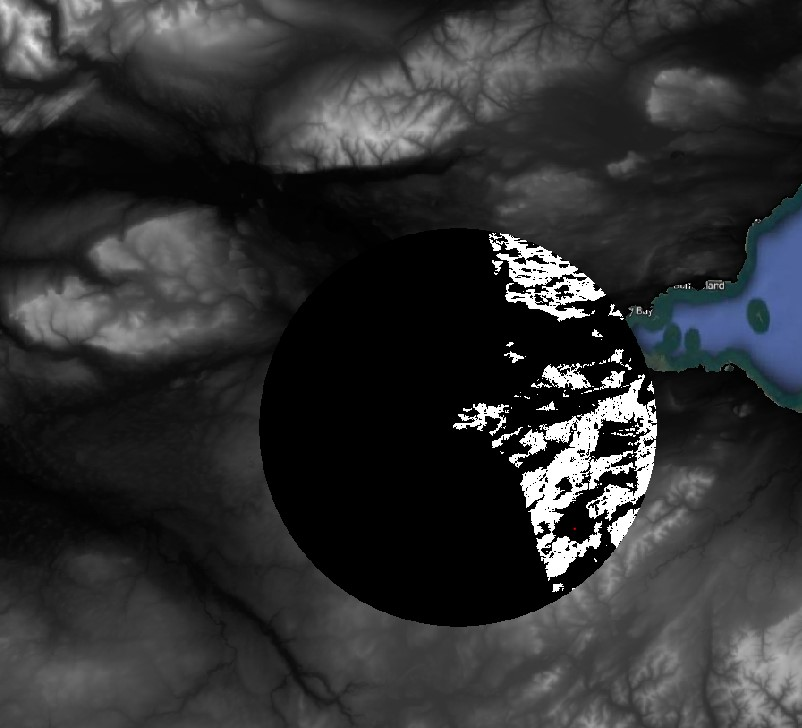
\includegraphics{images/lab_5/lab5_fig8_viewshed.jpg} \#\# Guided
Exercise 6 - Cleaning up and saving your project for the next lab

We will use the data you produced on this lab to get started on the
next, so let us 'package'it properly.

\begin{enumerate}
\def\labelenumi{(\arabic{enumi})}
\setcounter{enumi}{156}
\item
  Remove all layers from the project except for the SRTM, CORINE,
  BIOCLIM and GADM layers that you have reprojected and masked for the
  GB island. Save your project
\item
  Delete all files from the folder except for the files for the four
  data layers above. If you saved the GB island vector as a shapefile,
  remember you need to keep all files with the same name but different
  extensions (\texttt{.shp}, \texttt{.shx}, \texttt{.dbf},
  \texttt{.prj})
\item
  On your systems file explorer, find the base folder for today's lab
  according to your organization, and right click on it. On Windows,
  choose \texttt{Compress\ to...} to create a zipfile containing your
  entire project. Name it as \texttt{lab\_5\_final\_results.zip} or
  something similar.
\item
  Now store this zipfile on your university's OneDrive or on some
  external drive, so that you can re-download it when you need it for
  the next session.
\end{enumerate}

Congratulations, you reached the end of Lab 5. You should now understand
the raster data model and how to mask it and style it. You have also
learned some common terrain analysis tools. In the next lab, we will
learn about the \texttt{Raster\ Calculator}, which fulfils the role of
both the \texttt{Field\ Calculator} and \texttt{Select\ by\ Attribute}
for rasters.

\chapter{Lab 6: The raster calculator and other rastery
bits}\label{sec-labras2}

In this lab, we will continue working with rasters, and will learn how
to do several new operations using them, including using the
all-powerful \emph{Raster Calculator}. We will also see the effects of
\emph{raster resampling} in practice.

\section{Before you start!}\label{before-you-start-4}

\begin{enumerate}
\def\labelenumi{\arabic{enumi}.}
\tightlist
\item
  Go through the Week 3 preparatory session on Canvas, and watch the
  seminar recording if you have missed it. Also make sure you have
  completed all labs prior to this one.
\end{enumerate}

\section{Guided Exercise 1 - Global raster
statistics}\label{guided-exercise-1---global-raster-statistics}

In this exercise, we will use the layers from the previous lab to learn
about raster statistics and the raster calculator.

\subsection{Recovering your data}\label{recovering-your-data}

At the end of last week's lab you saved the final results of your
project as a zipfile. Retrieve this file, extract the contents, and
re-open your project. It should have these four layers in it:

\begin{itemize}
\tightlist
\item
  Polygon vector layer of the Island of Great Britain
\item
  Raster layer of the SRTM digital elevation model (reprojected to
  EPSG:27700 and masked to the GB island)
\item
  Raster file of the CORINE land cover dataset (reprojected to
  EPSG:27700 and masked to the GB island)
\item
  Raster file of the BIOCLIM climatic dataset (reprojected to EPSG:27700
  and masked to the GB island)
\end{itemize}

(if this doesn't work, I have a copy of the files
\href{https://stir-my.sharepoint.com/:u:/g/personal/ala2_stir_ac_uk/Eb28YoDGBM9MlraOgrbiehcBv9Q8BulLcloDNVypXmCUBw?e=DZfrqZ}{here}.
But you should \emph{really} try to make it work with your own saved
data - storing and retrieving project data is a key skill you need to
develop!)

\subsection{Global raster statistics}\label{global-raster-statistics}

Winter is coming, and you want to escape the worst of the cold and rain.
You therefore decide to use your GIS skills to find the ideal place to
spend your winter in the UK - an urban area with lower precipitation and
higher minimum temperatures. For convenience, we will restrict our
search to the Island of Great Britain (i.e.~`the main big island'), as
we already have data for it ready to go.

To get started, you would like to know what the overall range of
precipitation and temperature values for the entire island is, using the
BIOCLIM data. If this was a vector dataset, you would use the
\texttt{Statistical\ Summary\ Tool} - but it is a raster. What would be
the equivalent operation?

\begin{enumerate}
\def\labelenumi{(\arabic{enumi})}
\setcounter{enumi}{160}
\item
  The tool we need is called \texttt{Raster\ Layer\ Statistics}, but it
  is \emph{not} located in the \texttt{Raster} menu. Instead, we need to
  launch the \texttt{Processing} panel (
  
\includegraphics{index_files/mediabag/processingAlgorithm.png}. This
  panel contains a lot of additional GIS functions, and we will use it
  often now.
\item
  Once you have the \texttt{Processing} panel open, you can either
  search for \texttt{Raster\ Layer\ Statistics} or find it under the
  \texttt{Raster\ analysis} heading. Double click on it to launch the
  tool window. It should look like this:
\end{enumerate}

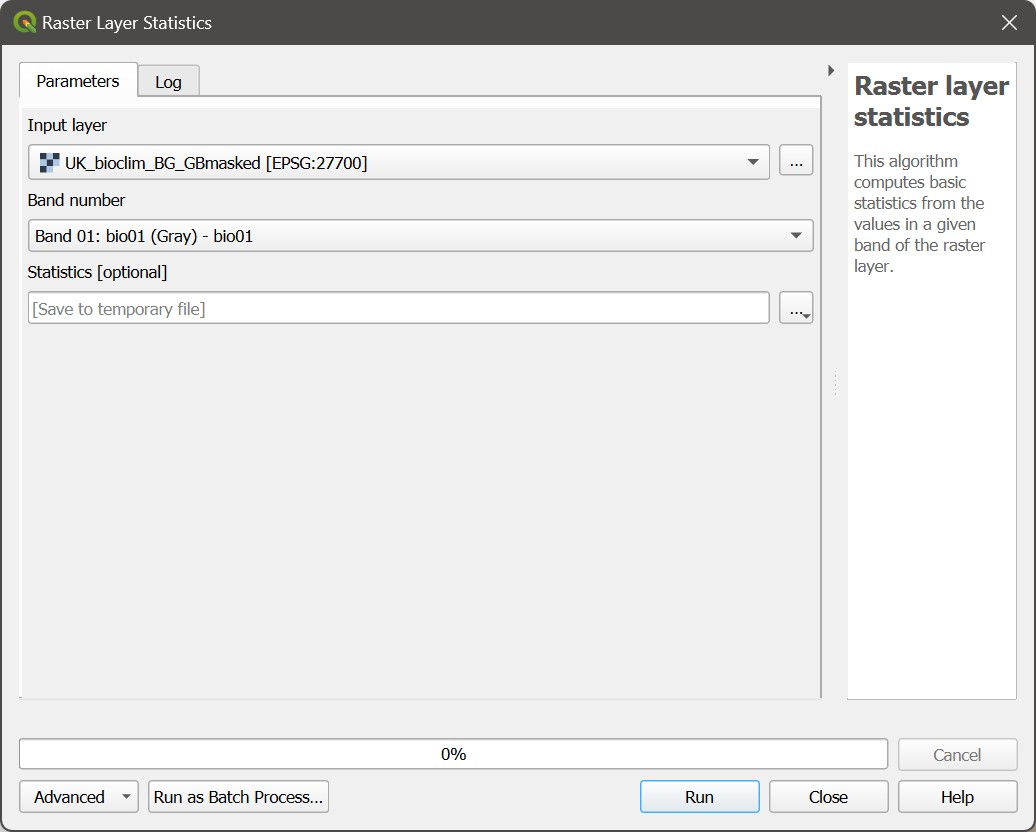
\includegraphics{images/lab_6/lab_6_fig1_rasterstats.jpg}

Looking at the BIOCLIM data description, the two useful pieces of
climatic data you need to get statistics for are \emph{BIO6 - Minimum
Temperature of the Coldest Month}, \emph{and BIO12 - Annual
Precipitation}. The BIO variables are ordered in the file, so \emph{band
6} is BIO6, and \emph{Band 12} is BIO12.

\begin{enumerate}
\def\labelenumi{(\arabic{enumi})}
\setcounter{enumi}{162}
\tightlist
\item
  In the \texttt{Raster\ Layer\ Statistics} window, select the BIOCLIM
  layer as \texttt{Input\ Layer} and \texttt{band\ 06} as band number.
  You can keep the results as a temporary file. \texttt{Run} it and
  \texttt{Close} the window. A new panel will have appeared under the
  \texttt{Processing} panel, called \texttt{Results\ Viewer}. It will
  have an entry called \texttt{Statistics}. Double click on it and take
  note of the minimum and maximum BIO6 values (-75 and 33).
\end{enumerate}

\begin{tcolorbox}[enhanced jigsaw, coltitle=black, toprule=.15mm, breakable, opacitybacktitle=0.6, left=2mm, colback=white, leftrule=.75mm, rightrule=.15mm, colbacktitle=quarto-callout-important-color!10!white, toptitle=1mm, titlerule=0mm, colframe=quarto-callout-important-color-frame, arc=.35mm, bottomtitle=1mm, opacityback=0, bottomrule=.15mm, title=\textcolor{quarto-callout-important-color}{\faExclamation}\hspace{0.5em}{Stop and Think}]

Do these values seem too extreme for the UK? What is going on here?

\end{tcolorbox}

\begin{tcolorbox}[enhanced jigsaw, toprule=.15mm, breakable, left=2mm, colframe=quarto-callout-important-color-frame, colback=white, arc=.35mm, leftrule=.75mm, opacityback=0, rightrule=.15mm, bottomrule=.15mm]

\vspace{-3mm}\textbf{Click for answer}\vspace{3mm}

The metadata for the BIO layers states that temperature values are
scaled by a factor of 10, so you need to divide these numbers by 10 to
get proper Celsius units.

\end{tcolorbox}

\begin{enumerate}
\def\labelenumi{(\arabic{enumi})}
\setcounter{enumi}{163}
\tightlist
\item
  Now repeat the process to get the Min and Max values for BIO12 (532
  and 2311)
\end{enumerate}

\begin{tcolorbox}[enhanced jigsaw, coltitle=black, toprule=.15mm, breakable, opacitybacktitle=0.6, left=2mm, colback=white, leftrule=.75mm, rightrule=.15mm, colbacktitle=quarto-callout-important-color!10!white, toptitle=1mm, titlerule=0mm, colframe=quarto-callout-important-color-frame, arc=.35mm, bottomtitle=1mm, opacityback=0, bottomrule=.15mm, title=\textcolor{quarto-callout-important-color}{\faExclamation}\hspace{0.5em}{Stop and Think}]

What are the units for precipitation?

\end{tcolorbox}

\begin{tcolorbox}[enhanced jigsaw, toprule=.15mm, breakable, left=2mm, colframe=quarto-callout-important-color-frame, colback=white, arc=.35mm, leftrule=.75mm, opacityback=0, rightrule=.15mm, bottomrule=.15mm]

\vspace{-3mm}\textbf{Click for answer}\vspace{3mm}

The metadata for the BIO layers states that annual precipitation is
given in mm. One millilitre of rain is equal to one litre per square
metre.

\end{tcolorbox}

\section{Guided Exercise 2 - Per-pixel calculations with the raster
calculator}\label{guided-exercise-2---per-pixel-calculations-with-the-raster-calculator}

Although it is easy enough to covert the temperature pixel values to
Celsius in our heads, it would be useful to have the data in the proper
units, especially if we want to map it later. Let us use the
\texttt{Raster\ Calculator} to apply the conversion factor to all
pixels.

\begin{enumerate}
\def\labelenumi{(\arabic{enumi})}
\setcounter{enumi}{164}
\tightlist
\item
  Go to the menu \texttt{Raster\ \textgreater{}\ Raster\ Calculator} to
  launch the calculator. It will look like this:
\end{enumerate}

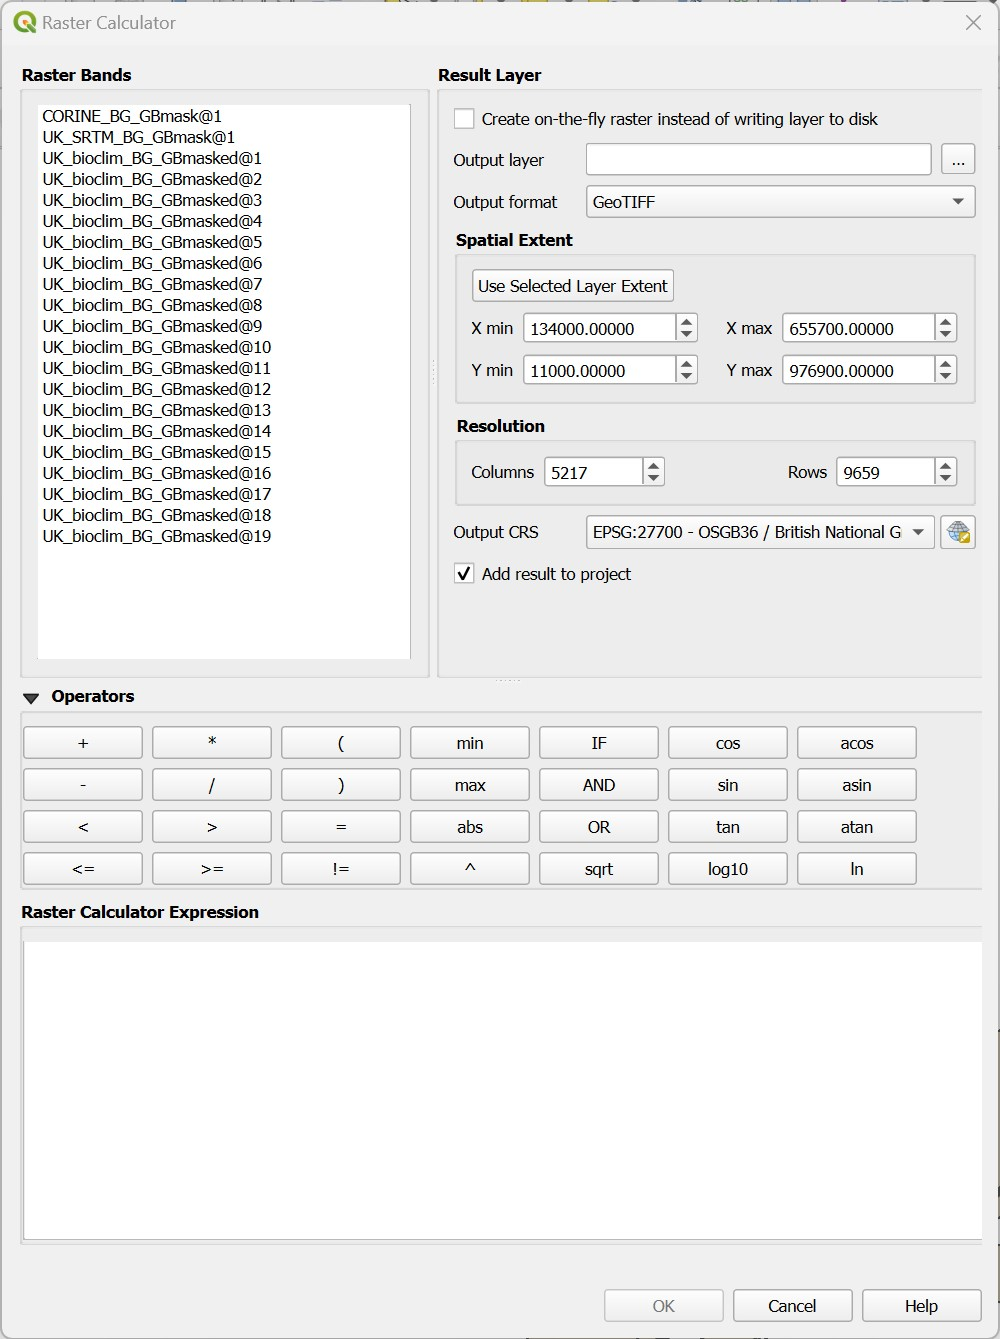
\includegraphics{images/lab_6/lab_6_fig2_rastercalc.jpg}

The general idea is similar to the \texttt{Field\ Calculator}, with a
slightly different layout. The top right panel lists all raster
\emph{bands} in the project (so \texttt{UK\_bioclim\_BG\_GBmasked@19}
means band 19 of the BIOCLIM raster). The top right panel lets us pick
some options for our raster creation, and the bottom panel lets us type
expressions.

\begin{enumerate}
\def\labelenumi{(\arabic{enumi})}
\setcounter{enumi}{165}
\item
  We need to divide all BIO6 temperature values by 10. Double click on
  the BIOCLIM band 6 in the bands list to add it to the expression
  panel, and then add the division by \texttt{10}. On my project, the
  final expression panel reads as
  \texttt{"UK\_bioclim\_BG\_GBmasked@6"\ /\ 10}, but your BIOCLIM layer
  may not be named the same as mine. Note that the bottom of the
  expression panel should say \texttt{Expression\ Valid}. If it says
  \texttt{Expression\ Invalid}, check your typing (did you use the
  double quotes?)
\item
  For \texttt{Output\ Layer}, click on the \texttt{...} button and pick
  a folder to save the new file. Name it
  \texttt{UK\_bioclim\_BG\_GBmasked\_BIO6\_celsius.tif}. Leave the rest
  as default and click in \texttt{OK}.
\end{enumerate}

\begin{tcolorbox}[enhanced jigsaw, coltitle=black, toprule=.15mm, breakable, opacitybacktitle=0.6, left=2mm, colback=white, leftrule=.75mm, rightrule=.15mm, colbacktitle=quarto-callout-important-color!10!white, toptitle=1mm, titlerule=0mm, colframe=quarto-callout-important-color-frame, arc=.35mm, bottomtitle=1mm, opacityback=0, bottomrule=.15mm, title=\textcolor{quarto-callout-important-color}{\faExclamation}\hspace{0.5em}{Stop and Think}]

How many bands does your newly created file have?

\end{tcolorbox}

\begin{tcolorbox}[enhanced jigsaw, toprule=.15mm, breakable, left=2mm, colframe=quarto-callout-important-color-frame, colback=white, arc=.35mm, leftrule=.75mm, opacityback=0, rightrule=.15mm, bottomrule=.15mm]

\vspace{-3mm}\textbf{Click for answer}\vspace{3mm}

Only one band, holding the results of the calculation.

\end{tcolorbox}

Every time you enter an expression involving a raster band and a single
number in the \texttt{Raster\ Calculator} you are telling QGIS to apply
the same expression to each pixel of that band. In our case, we divided
all pixel values by 10.

\section{Guided Exercise 3 - Boolean (logical) operations with the
raster
calculator}\label{guided-exercise-3---boolean-logical-operations-with-the-raster-calculator}

The \texttt{Raster\ Calculator} also fulfils the role of the vector
\texttt{Select\ by\ expression} tool for rasters. The result of any
raster logical operation is either \texttt{1} (True) or \texttt{0}
(False), i.e.~a \emph{binary raster}, sometimes called a \emph{raster
mask}.

Let us find the warmer places in Great Britain. Our highest minimum
temperature of the coldest month (BIO6) value was 3.3 degrees, not too
far from zero. So let us limit our search to any places that don't go
below 0 Celsius.

\begin{enumerate}
\def\labelenumi{(\arabic{enumi})}
\setcounter{enumi}{167}
\tightlist
\item
  Open the \texttt{Raster\ Calculator} again, and this time use the
  expression
  \texttt{"UK\_bioclim\_BG\_GBmask\_BIO6\_celsius@1"\ \textgreater{}\ 0}.
  Notice we used here the layer that we just converted to degrees
  Celsius. Save the results in a proper folder with the name
  \texttt{GB\_mintemp\_gt\_0.tif} (gt for `greater than') and run the
  calculation. You should get something like this:
\end{enumerate}

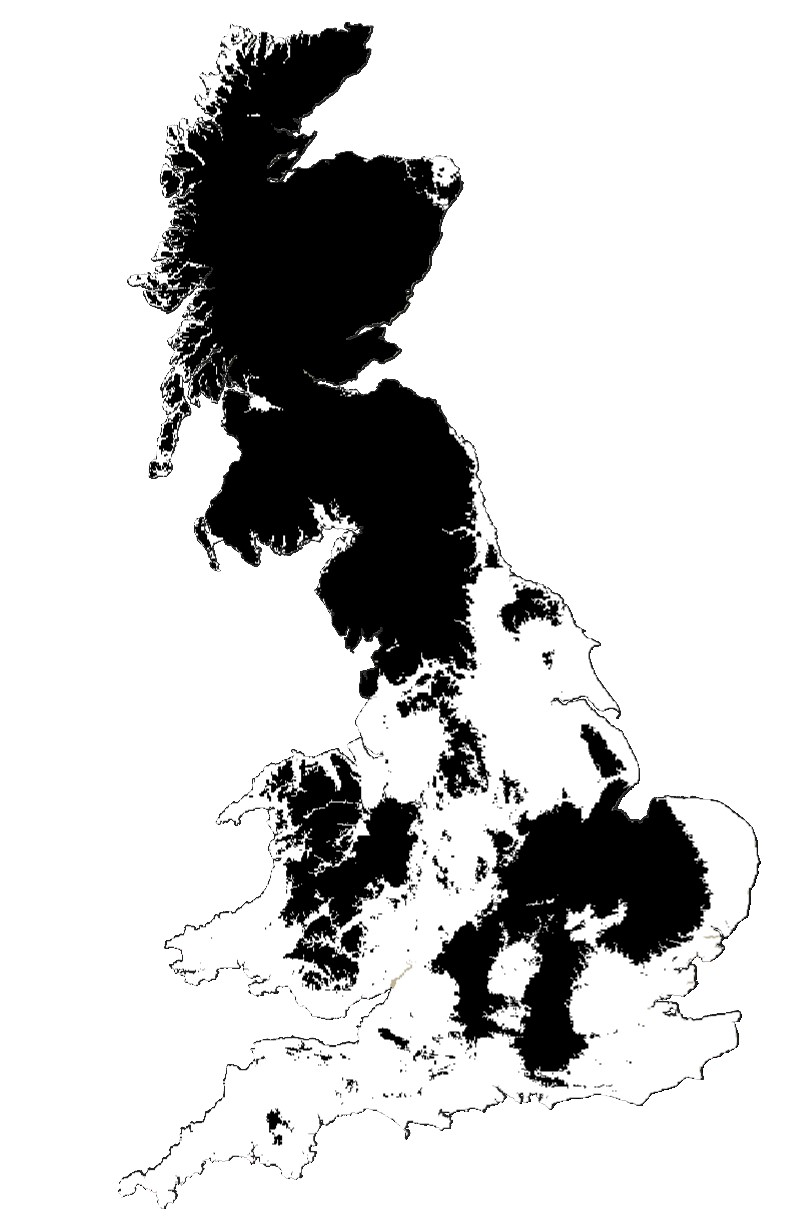
\includegraphics{images/lab_6/lab_6_fig3_mintemp_gt_0.jpg} By default,
QGIS will paint pixels with a value of \texttt{1} white, and \texttt{2}
black. So the white areas now show us all regions of Great Britain that
\emph{on average} don't go below zero in the worst of winter (these are
long term climatic averages). Use the \texttt{Identify\ Features} tool
to check if the pixel values are really \texttt{0} and \texttt{1}.

\begin{enumerate}
\def\labelenumi{(\arabic{enumi})}
\setcounter{enumi}{168}
\tightlist
\item
  Now repeat the process for the precipitation layer. Our minimum annual
  precipitation value was just above 500, so let us limit our search to
  areas under 700mm of precipitation. Save the result as
  \texttt{GB\_anprec\_lt\_700.tif}.
\end{enumerate}

\section{Guided Exercise 4 - Raster
reclassification}\label{guided-exercise-4---raster-reclassification}

An alternative to the \texttt{Raster\ Calculator} that can be handier
when you have multiple ranges to recode is the
\texttt{Reclassify\ by\ table} tool in the \texttt{Processing} panel,
also under the \texttt{Raster\ Analysis} heading. Find the tool and open
it, and you will see this:

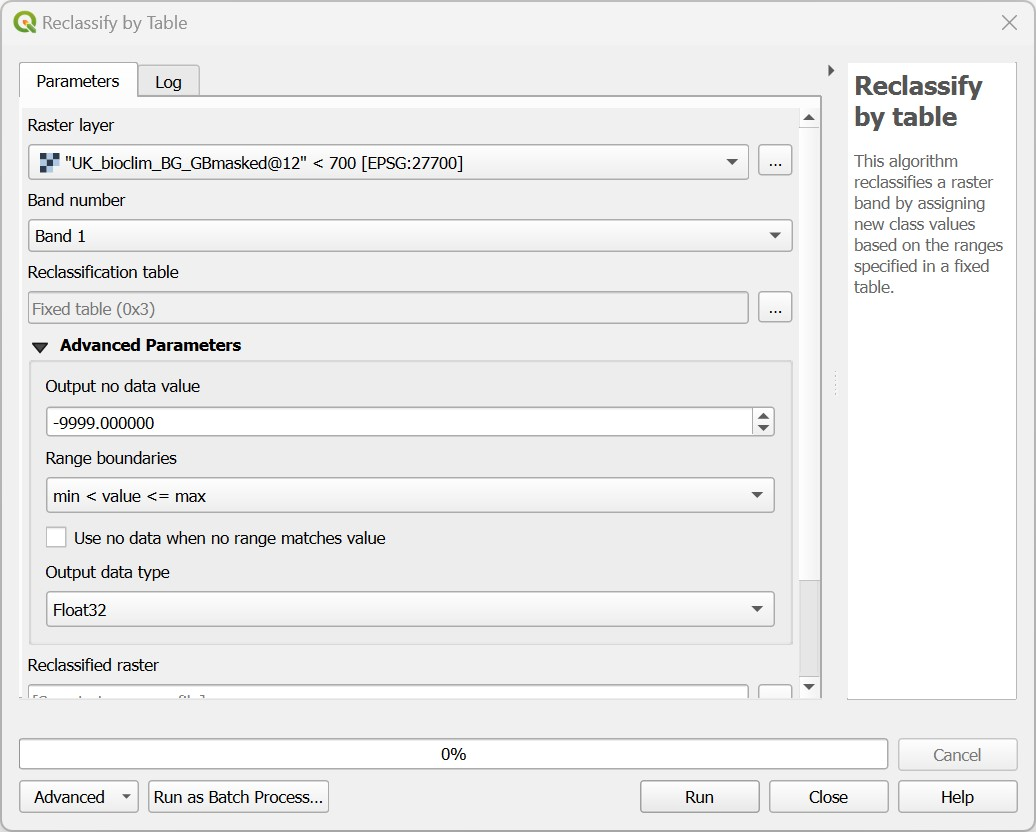
\includegraphics{images/lab_6/lab_6_fig4_rec_by_table.jpg}

Let us use this tool to extract the urban areas from the CORINE dataset.
looking at the metadata, the two classes of interest are
\texttt{Continuous\ Urban\ Fabric} (pixel value 111) and
\texttt{Discontinuous\ Urban\ Fabric} (112) classes, which are the
classes were we would expect existing housing to be located.

\begin{enumerate}
\def\labelenumi{(\arabic{enumi})}
\setcounter{enumi}{169}
\tightlist
\item
  On the \texttt{Reclassify\ by\ table} window, pick the CORINE layer as
  your \texttt{Raster\ layer}, and \texttt{band\ 1} as your
  \texttt{Band\ Number}. Then click on the \texttt{...} button besides
  the box to open the \texttt{Reclassification\ \ table}, and fill the
  table like the figure below. Click to add rows as necessary.
\end{enumerate}

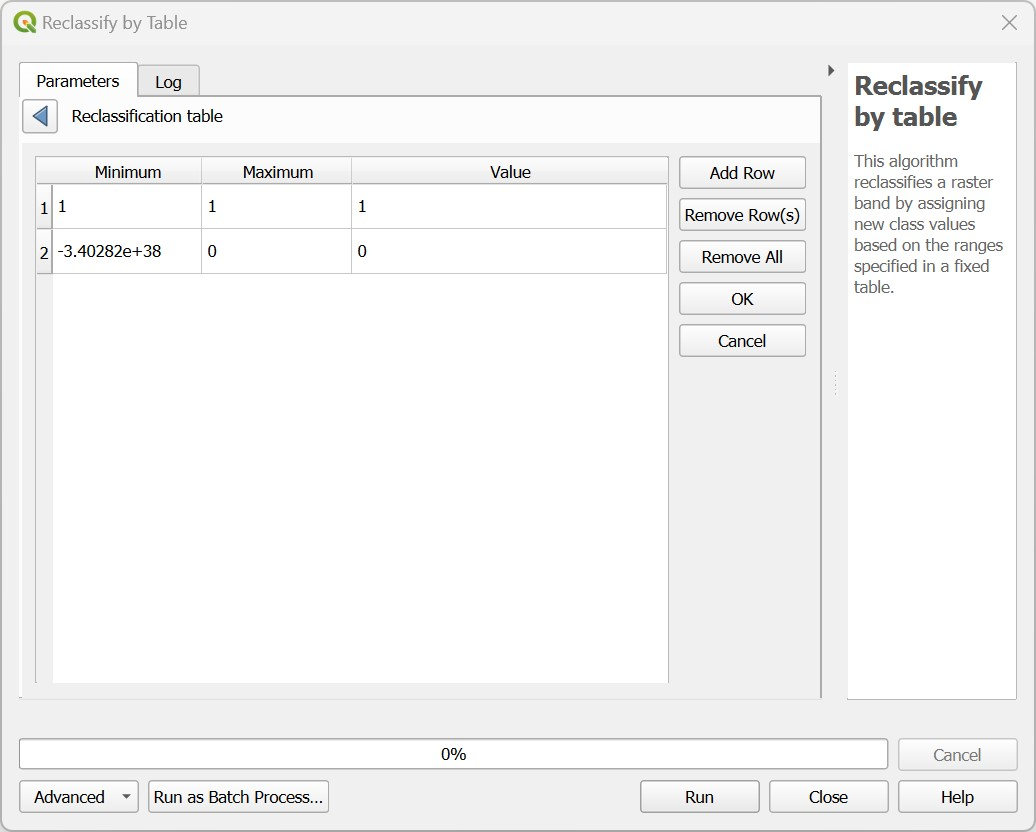
\includegraphics{images/lab_6/lab_6_fig5_rec_table.jpg}

\begin{enumerate}
\def\labelenumi{(\arabic{enumi})}
\setcounter{enumi}{170}
\tightlist
\item
  Click on the blue arrow to go back to main tool window, then set the
  \texttt{nodata\ value} back to \texttt{-32768}, the
  \texttt{Range\ Boundaries} to
  \texttt{min\ \textless{}=\ value\ \textless{}=\ max} and the
  \texttt{Output\ Data\ Type} to \texttt{Byte}. Save it as
  \texttt{GB\_urban\_areas.tif}.
\end{enumerate}

\begin{tcolorbox}[enhanced jigsaw, coltitle=black, toprule=.15mm, breakable, opacitybacktitle=0.6, left=2mm, colback=white, leftrule=.75mm, rightrule=.15mm, colbacktitle=quarto-callout-important-color!10!white, toptitle=1mm, titlerule=0mm, colframe=quarto-callout-important-color-frame, arc=.35mm, bottomtitle=1mm, opacityback=0, bottomrule=.15mm, title=\textcolor{quarto-callout-important-color}{\faExclamation}\hspace{0.5em}{Stop and Think}]

How could you have done the analysis above using the
\texttt{Raster\ Calculator} instead?

\end{tcolorbox}

\begin{tcolorbox}[enhanced jigsaw, toprule=.15mm, breakable, left=2mm, colframe=quarto-callout-important-color-frame, colback=white, arc=.35mm, leftrule=.75mm, opacityback=0, rightrule=.15mm, bottomrule=.15mm]

\vspace{-3mm}\textbf{Click for answer}\vspace{3mm}

You could do
\texttt{"CORINE\_BG\_GBmask@1"\ =\ 111\ OR\ "CORINE\_BG\_GBmask@1"\ =\ 112}.
Notice how you can use \texttt{AND} and \texttt{OR} to chain logical
expressions as you can for vectors - but because computers are dumb, you
need to repeat the name of the layer after the \texttt{OR} (and for each
additional expression you add).

You could also do ranges, using an expression such as
\texttt{"CORINE\_BG\_GBmask@1"\ \textgreater{}\ 110\ AND\ "CORINE\_BG\_GBmask@1"\ \textless{}\ 113}
(notice the use of \texttt{AND} instead of \texttt{OR} for ranges) since
they are consecutive values, or use
\texttt{"CORINE\_BG\_GBmask@1"\ \textgreater{}=111\ AND\ "CORINE\_BG\_GBmask@1"\ \textless{}=\ 112}).
Using ranges is quicker than using \texttt{=} and \texttt{OR} when you
have many consecutive values to search for.

\end{tcolorbox}

\section{Guided Exercise 5 - raster vs.~raster
calculations}\label{guided-exercise-5---raster-vs.-raster-calculations}

We now have three \emph{raster masks} showing us 1) all the GB areas
that don't go below zero Celsius, 2) the areas that have less than 700mm
of rain, and 3) the areas that are urban. How can we combine them into a
single layer?

The answer to the above question is still the
\texttt{Raster\ Calculator}. We know the pixels we `want' are numbered
\texttt{1} on each layer, otherwise they are \texttt{0}. So if we could
multiply one layer by the other, i.e.~multiply the value of each set of
overlapping pixels, we would get a new raster with values of
\(1 \times 1 \times 1 = 1\) when both conditions are met, and a result
of \(0\) if any of the conditions is not met. This is why binary rasters
are also called raster \emph{masks} - when you multiply any other raster
by it, it \emph{masks} (i.e.~zeroes out) anything that is not
\texttt{True} in the mask.

Doing it using the \texttt{Raster\ Calculator} is as simple as it
sounds:

\begin{enumerate}
\def\labelenumi{(\arabic{enumi})}
\setcounter{enumi}{171}
\tightlist
\item
  Open the \texttt{Raster\ Calculator} and enter the expression
  \texttt{"GB\_anprec\_lt\_700@1"\ *\ "GB\_mintemp\_gt\_0@1"\ *\ GB\_urban\_areas@1}.
  Then save you layer with name \texttt{UKs\_winter\_havens.tif}.
\end{enumerate}

\section{Guided Exercise 6 - Vectorizing
rasters}\label{guided-exercise-6---vectorizing-rasters}

The final result of your analysis should consist of only a handful of
pixels - such is life in the UK. And since these are discrete locations,
it may occur to you they would be better represented and visualised as
vectors. Turns out we can convert raster to vectors and vice versa:

\begin{enumerate}
\def\labelenumi{(\arabic{enumi})}
\setcounter{enumi}{172}
\item
  Go to
  \texttt{Raster\ \textgreater{}\ Conversion\ \textgreater{}\ Polygonize\ (Raster\ to\ Vector)...}.
  In the new window, pick your results layer as the
  \texttt{Input\ Layer}, \texttt{Band\ 1} as the \texttt{Band\ number},
  and leave the rest as default (\texttt{DN} here means \emph{digital
  number}, another name for pixel values. Then pick a folder and save
  the results as \texttt{UK\_winter\_havens\_poly.shp} (or geopackage if
  you prefer).
\item
  You will notice that a very large polygon was also created for the 0
  areas of the raster. You can then put the new vector layer in editing
  mode, use the \texttt{Selection\ Tool} to select this polygon, and
  then hit the \texttt{Delete} key on your keyboard to get rid of it.
  Then save the changes and exit edit mode.
\end{enumerate}

\begin{tcolorbox}[enhanced jigsaw, coltitle=black, toprule=.15mm, breakable, opacitybacktitle=0.6, left=2mm, colback=white, leftrule=.75mm, rightrule=.15mm, colbacktitle=quarto-callout-warning-color!10!white, toptitle=1mm, titlerule=0mm, colframe=quarto-callout-warning-color-frame, arc=.35mm, bottomtitle=1mm, opacityback=0, bottomrule=.15mm, title=\textcolor{quarto-callout-warning-color}{\faExclamationTriangle}\hspace{0.5em}{Warning}]

Polygonising rasters can be a very computationally-heavy operation if
you have large rasters and/or many scattered pixel values (for example,
vectorising the original CORINE layer with all classes). And it is
virtually useless for continuous rasters such as temperature or
elevation (you would end up with one polygon per pixel as there would be
no adjacent pixels with the same value).

So if you start an analysis with raster data, try to do as much as you
can in the raster domain, before vectorising anything. But if your
raster results represent isolated small regions within a large matrix of
`no data' or zero values, then vectorising is a good idea.

\end{tcolorbox}

You now have polygons representing all adjacent areas that were values
as `1' in your raster. But many of them are still only one pixel. What
if you wanted to have points instead of polygons?

\begin{enumerate}
\def\labelenumi{(\arabic{enumi})}
\setcounter{enumi}{174}
\tightlist
\item
  In the \texttt{Processing} panel, you will find a tool called
  \texttt{Raster\ Pixels\ to\ Points}, which you can use to generate the
  points. I'll leave the details to you, but here is a tip: before you
  use the tool, go the \texttt{Properties\ \textgreater{}\ Transparency}
  of your raster results layer, and set 0 as an
  \texttt{Additional\ Nodata\ Value}. Otherwise
  \texttt{Raster\ Pixels\ to\ Points} will create one point for every
  pixel, including the pixels with a value of 0. That's a lot of points.
\end{enumerate}

\section{Guided Exercise 7 - Mosaicking and Stacking
rasters}\label{guided-exercise-7---mosaicking-and-stacking-rasters}

Raster files are often very large and `heavy', so it is common to
distribute them as \emph{tiles} or \emph{scenes}, i.e.~smaller adjacent
pieces that can be merged back together to cover a certain area of
interest. For satellite images, it is also common for each image band to
be stored as a separate file (unlike regular photos that only have Blue,
Red and Green bands, satellite images can have several more bands,
covering areas of the spectrum we can't normally see. The Sentinel-2
satellite, for example, has a total of 13 bands:

\begin{longtable}[]{@{}lll@{}}
\toprule\noalign{}
Band & Wavelength & Description \\
\midrule\noalign{}
\endhead
\bottomrule\noalign{}
\endlastfoot
B1 & 443 nm & Ultra Blue (Coastal and Aerosol) \\
B2 & 490 nm & Blue \\
B3 & 560 nm & Green \\
B4 & 665 nm & Red \\
B5 & 705 nm & Visible and Near Infrared (VNIR) \\
B6 & 740 nm & Visible and Near Infrared (VNIR) \\
B7 & 783 nm & Visible and Near Infrared (VNIR) \\
B8 & 842 nm & Visible and Near Infrared (VNIR) \\
B8a & 865 nm & Visible and Near Infrared (VNIR) \\
B9 & 940 nm & Short Wave Infrared (SWIR) \\
B10 & 1375 nm & Short Wave Infrared (SWIR) \\
B11 & 1610 nm & Short Wave Infrared (SWIR) \\
B12 & 2190 nm & Short Wave Infrared (SWIR) \\
\end{longtable}

In this exercise, we will learn how to a) \emph{mosaic} rasters - `glue'
them together side by side to cover a larger area and b) \emph{stack}
rasters - merge the different band files into a single file.

\begin{enumerate}
\def\labelenumi{(\arabic{enumi})}
\setcounter{enumi}{175}
\tightlist
\item
  \href{https://stir-my.sharepoint.com/:u:/g/personal/ala2_stir_ac_uk/EWWIMudbgUlImqIZ5ZYoVw4BNhL1rRn5swLLTvJnli2r_A?e=NIVOuW}{Download
  the data for this specific exercise from this link}. It contains four
  aerial photographs covering the University of Stirling campus and the
  Wallace Monument area. Extract the data and organise it as usual.
\end{enumerate}

\begin{tcolorbox}[enhanced jigsaw, coltitle=black, toprule=.15mm, breakable, opacitybacktitle=0.6, left=2mm, colback=white, leftrule=.75mm, rightrule=.15mm, colbacktitle=quarto-callout-tip-color!10!white, toptitle=1mm, titlerule=0mm, colframe=quarto-callout-tip-color-frame, arc=.35mm, bottomtitle=1mm, opacityback=0, bottomrule=.15mm, title=\textcolor{quarto-callout-tip-color}{\faLightbulb}\hspace{0.5em}{Tip}]

These images were originally downloaded from the `Aerial' section of
Digimap - if you ever need very detailed imagery within the UK, check it
out!

\end{tcolorbox}

\begin{enumerate}
\def\labelenumi{(\arabic{enumi})}
\setcounter{enumi}{176}
\tightlist
\item
  Each image is stored within its own folder, named \texttt{nsXXXX},
  where \texttt{XXXX} is a four digit number. \emph{Start a new project}
  and load into QGIS all the \texttt{.tif} files in all four folders.
  There should be six files in total.
\end{enumerate}

\begin{tcolorbox}[enhanced jigsaw, coltitle=black, toprule=.15mm, breakable, opacitybacktitle=0.6, left=2mm, colback=white, leftrule=.75mm, rightrule=.15mm, colbacktitle=quarto-callout-important-color!10!white, toptitle=1mm, titlerule=0mm, colframe=quarto-callout-important-color-frame, arc=.35mm, bottomtitle=1mm, opacityback=0, bottomrule=.15mm, title=\textcolor{quarto-callout-important-color}{\faExclamation}\hspace{0.5em}{Stop and Think}]

What do you think is the meaning of the \texttt{nsXXXX} folder names?

\end{tcolorbox}

\begin{tcolorbox}[enhanced jigsaw, toprule=.15mm, breakable, left=2mm, colframe=quarto-callout-important-color-frame, colback=white, arc=.35mm, leftrule=.75mm, opacityback=0, rightrule=.15mm, bottomrule=.15mm]

\vspace{-3mm}\textbf{Click for answer}\vspace{3mm}

They indicate tiles in the OS British Grid system.

\end{tcolorbox}

Notice that the airphoto for tile ns8196 has been provided with its
three colour bands (RGB) as separate files - simulating what you would
expect for satellite files. To be able to see this aerial photo in
colour, we must first \emph{stack} these bands into a single file. The
operation is called \emph{stack} because you could visualise it as
physically stacking them one on top of the other.

\begin{enumerate}
\def\labelenumi{(\arabic{enumi})}
\setcounter{enumi}{177}
\tightlist
\item
  Go to
  \texttt{Raster\ \textgreater{}\ Miscellaneous\ \textgreater{}\ Merge...}.
  You will get a window like this:
\end{enumerate}

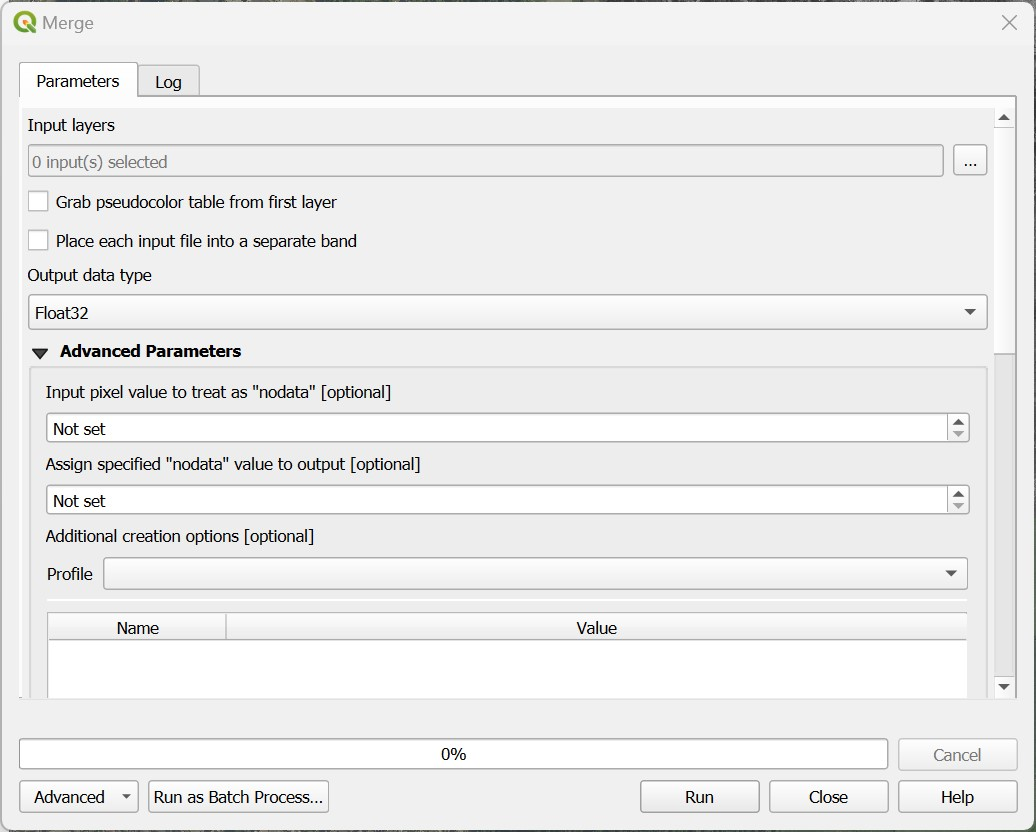
\includegraphics{images/lab_6/lab_6_fig6_merge.jpg} (@) For
\texttt{Input\ Layers}, click on the \texttt{...} button, and a list of
all available raster layers in your project will appear. You can drag
the layer names to reorder them, and your final selection should the
\texttt{ns8196\_R}, \texttt{ns8196\_G}, and \texttt{ns8196\_B} layers,
in the order below from top to bottom. This sets the order of the bands
inside the file.

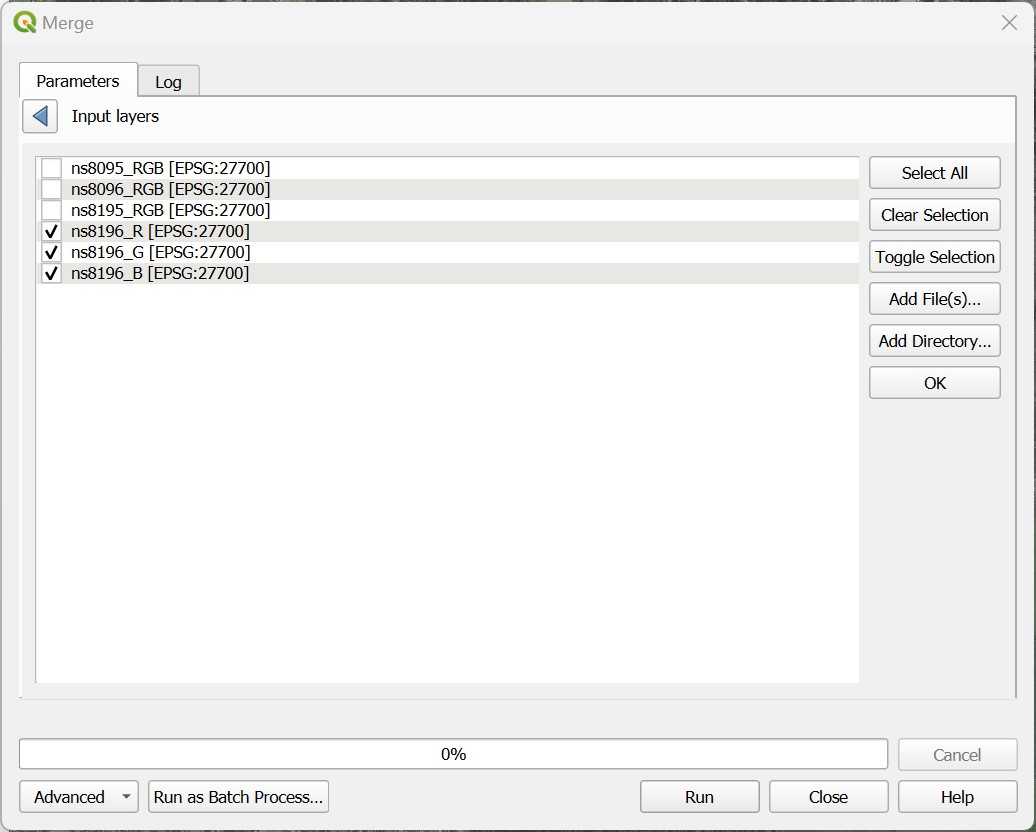
\includegraphics{images/lab_6/lab_6_fig7_merge_layers.jpg} (@) Once you
have selected the layers, click on the blue arrow to go back to the main
window, then set the following parameters: \emph{check the box} for
\texttt{Place\ each\ input\ file\ into\ a\ separate\ band} (that tells
QGIS you want a \emph{stack}), and the \texttt{Output\ Data\ Type} to
\texttt{Byte}. Then save the resulting file as \texttt{ns8196\_RGB.tif},
in the same folder where you had the three separate band files.

\begin{tcolorbox}[enhanced jigsaw, coltitle=black, toprule=.15mm, breakable, opacitybacktitle=0.6, left=2mm, colback=white, leftrule=.75mm, rightrule=.15mm, colbacktitle=quarto-callout-important-color!10!white, toptitle=1mm, titlerule=0mm, colframe=quarto-callout-important-color-frame, arc=.35mm, bottomtitle=1mm, opacityback=0, bottomrule=.15mm, title=\textcolor{quarto-callout-important-color}{\faExclamation}\hspace{0.5em}{Stop and Think}]

Why do we change \texttt{Output\ Data\ Type} to \texttt{Byte}?

\end{tcolorbox}

\begin{tcolorbox}[enhanced jigsaw, toprule=.15mm, breakable, left=2mm, colframe=quarto-callout-important-color-frame, colback=white, arc=.35mm, leftrule=.75mm, opacityback=0, rightrule=.15mm, bottomrule=.15mm]

\vspace{-3mm}\textbf{Click for answer}\vspace{3mm}

The RGB colour system uses one byte (8-bits, 0-255 integer numbers) per
colour channel to designate any colour. For example, the University of
Stirling official green colour
(
\includegraphics{images/lab_6/lab_6_fig9_StirColor.jpg}) is R=0 G=105
B=56. The \texttt{Byte} option ensures we only use 8-bits per band, and
keep the file size smaller. If we left it as \texttt{Float32}, the same
0-225 integer numbers would be stored as 32-bit decimal numbers,
quadrupling the size of the file for no reason.

\end{tcolorbox}

\begin{enumerate}
\def\labelenumi{(\arabic{enumi})}
\setcounter{enumi}{178}
\tightlist
\item
  You should now have a properly coloured image for tile ns8196. Remove
  the three original single band layers from the project and then save
  it.
\end{enumerate}

Everything looks good colour-wise now, bur our airphoto is still
actually four separate adjacent photos. That means any processing we may
want to do involving the entire area would have to be repeated four
times. We can however merge these four tiles in a single airphoto
\emph{mosaic}.

\begin{enumerate}
\def\labelenumi{(\arabic{enumi})}
\setcounter{enumi}{179}
\item
  Go back to
  \texttt{Raster\ \textgreater{}\ Miscellaneous\ \textgreater{}\ Merge...}.
  Yes, it is a bit confusing, QGIS uses the same tool for both stacking
  and mosaicking.
\item
  This time, check the four tiled RGB images as your
  \texttt{Input\ Layers} - order doesn't matter. Then make sure to
  \textbf{not check} the
  \texttt{Place\ each\ input\ file\ into\ a\ separate\ band} option.
  That will tell QGIS you want a mosaic and not a stack. Set the
  \texttt{Output\ Data\ Type} to \texttt{Byte} again, and save it as
  \texttt{UoS\_RGB\_mosaic.tif}. You should now have a single airphoto
  layer covering the entire area. Remove the previous individual layers
  from the project and save it again.
\end{enumerate}

\section{Guided Exercise 8 - Raster image
stretching}\label{guided-exercise-8---raster-image-stretching}

When working with multiband color images in a GIS environment, we can
often manipulate the contrast of an image by applying different
\emph{contrast stretches} to each band. Especially when working with
satellite images, which tend to look a bit `faded' because of the
atmospheric effect, stretching can make our images more vivid and easier
to interpret.

\begin{enumerate}
\def\labelenumi{(\arabic{enumi})}
\setcounter{enumi}{181}
\tightlist
\item
  Right-click on the airphoto mosaic layer you created and go to
  \texttt{Properties\ \textgreater{}\ Symbology}. You will see that the
  symbology type is \texttt{Multiband\ color}, which is the correct
  choice for representing images. Note that each band is associated to a
  colour channel (R, G, B), but this association can be changed at will.
  Change the \texttt{Red\ band} to band 2, and the \texttt{Green\ band}
  to band 1, then \texttt{Apply}. Now the vegetation appears red! Change
  it back to the proper colour order and \texttt{Apply} again.
\end{enumerate}

\begin{tcolorbox}[enhanced jigsaw, coltitle=black, toprule=.15mm, breakable, opacitybacktitle=0.6, left=2mm, colback=white, leftrule=.75mm, rightrule=.15mm, colbacktitle=quarto-callout-tip-color!10!white, toptitle=1mm, titlerule=0mm, colframe=quarto-callout-tip-color-frame, arc=.35mm, bottomtitle=1mm, opacityback=0, bottomrule=.15mm, title=\textcolor{quarto-callout-tip-color}{\faLightbulb}\hspace{0.5em}{Tip}]

This is a useful feature when working with satellite images, which often
have bands representing spectral regions that we cannot see, such as
Near Infrared or Microwave. We can then freely associate these bands to
colour channels and create \texttt{false\ colour\ compositions} that
highlight different surface features. The example below shows the UoS
campus as seen from the Sentinel-2 satellite. Here we place Band 13 -
Short Wave Infrared (SWIR) in the blue channel, Band 8 - Near-Infrared
band (NIR) in the green channel, and Band 11 - SWIR in the red channel.
Since water does not reflect IR, the loch appears black. Plants reflect
strongly in the NIR region so they appear bright green, and bare ground
/ concrete reflects mostly in the SWIR, thus appearing purplish
(red+blue).

\includegraphics{images/lab_6/lab_6_fig10_StirSentinel.jpg}

\end{tcolorbox}

\begin{enumerate}
\def\labelenumi{(\arabic{enumi})}
\setcounter{enumi}{182}
\item
  Notice how the \texttt{Min} and \texttt{Max} values for each band are
  \texttt{0} and \texttt{255}, meaning we are mapping our screen colours
  to the entire range of possible values (0-255). But quite often the
  colours in an image do not cover the entire 8-bit range, so we are
  `wasting' colour discrimination.
\item
  Change the \texttt{No\ Enhancement} option to
  \texttt{Stretch\ to\ Min/Max}, and then expand the
  \texttt{Min/Max\ Value\ Settings} heading. Pick the \texttt{Min/Max}
  option, and select \texttt{Whole\ Raster} for
  \texttt{Statistics\ Extent} and \texttt{Actual(slower)} for
  \texttt{Accuracy}, then click on \texttt{Apply}. You will see that
  while band 1 and band 3 do use the entire 0-255 range, band 2 uses the
  2-255 range only.
\end{enumerate}

To further enhance the contrast of images, we can tell QGIS to `cut off'
the extreme values of the range, using different methods.

\begin{enumerate}
\def\labelenumi{(\arabic{enumi})}
\setcounter{enumi}{184}
\item
  Change the \texttt{Min/Max\ Value\ Settings} option to
  \texttt{Cumulative\ Count\ Cut}, and then\texttt{Apply}. Now the
  \texttt{Min} and \texttt{Max} colour values for each band are (13-189,
  29-187,and 31-164 respectively), and the image should look more vivid.
  What QGIS did was remove the values in the lowest 2\% (0.2 percentile)
  and highest 2\% (0.98 percentile) of the existing range before
  calculating Min/Max values, thus \emph{stretching} this smaller number
  range to the full colour range of the screen.
\item
  Progressively increase the lower percentile (i.e.~from 2\% to 3\%) and
  decrease the upper percentile (i.e.~from 98\% to 97\%) and notice how
  the contrast gets progressively stronger. If you go too far (i.e.~too
  narrow a range) you will start to see \emph{pixel saturation} - many
  of the pixels will be outside the range and thus mapped to fully black
  or fully white.
\end{enumerate}

A second way to calculate the stretch is to use standard deviations. You
may remember from statistics that when you assume a Normal distribution,
a distance of \(\pm 1 \sigma\) from the mean will capture about 68\% of
the data, \(\pm 2 \sigma\) will capture 98\%, \(\pm 3 \sigma\) will
capture X \% and so on:

\includegraphics{images/lab_6/lab_6_fig11_normal.jpg}

\begin{enumerate}
\def\labelenumi{(\arabic{enumi})}
\setcounter{enumi}{186}
\item
  Change the \texttt{Min/Max\ Value\ Settings} option to
  \texttt{Mean\ +/-\ Standard\ Deviation\ x}, and leave the multiplier
  at \texttt{2}. Apply and check the contrast. Then change the
  multiplier to \texttt{1} and \texttt{Apply}, and compare the contrast
  of using \(\pm 1 \sigma\) vs.~\(\pm 2 \sigma\).
\item
  Set the final image contrast to your liking and exit the
  \texttt{Properties} window. Save your project.
\end{enumerate}

\subsection{Independent Exercise - Raster
resampling}\label{independent-exercise---raster-resampling}

As you have learned, raster data consists of a \emph{grid} of pixel
values (i.e.~a matrix). So quite often, when working with rasters, you
may need to shift the pixels from one grid to another. One main example
is raster reprojection - if you reproject your raster to a different
CRS, the new raster grid will be aligned with this new CRS, and won't
match the original perfectly, as in the figure below.

\includegraphics{images/lab_6/lab_6_fig14_mismatched_grids.jpg}

That is why the raster reprojection tool is called
\texttt{Warp(Reproject)} - it is as if you are \emph{warping} the image
during the transformation. Other times you may need to make two
different raster datasets match the same extent and pixel size, which
would also require warping one of the rasters to match the other.

A key step when doing these transformations is choosing a
\emph{resampling} method, i.e.~in which way will the original pixel
values be transferred to the new grid. The most common and fast method
is called \emph{Nearest Neighbour} (NN) - if you imagine the old and new
grids partially overlapping, NN resampling just looks for the closest
old pixel to the new pixel, and transfers the value:

\includegraphics{images/lab_6/lab_6_fig12_NN.jpg} NN is fast because it
requires no additional computations, and also has the benefit of not
changing the original data values. But if your data has a lot of fine
and/or linear elements, it may result in a `jagged' appearance. For that
reason, other methods exist that try to \emph{interpolate} the new pixel
values based on a combination of the original ones. Two common methods
are the \emph{bilinear} and \emph{bicubic} interpolations, which will
average the 4 and 16 closest pixels, respectively. That has the benefit
of creating smoother resulting rasters:

\begin{figure}[H]

{\centering \includegraphics{images/lab_6/lab_6_fig13_resamps.jpg}

}

\caption{Source:10.13140/RG.2.2.16038.27207}

\end{figure}%

Let us now practice our raster skills in an independent exercise, while
also demonstrating the effect of resampling:

\begin{enumerate}
\def\labelenumi{\arabic{enumi}.}
\tightlist
\item
  On your UK SRTM layer, find the location of Stirling and the
  university campus, and then use the
  \texttt{Raster\ \textgreater{}\ Extraction\ \textgreater{}\ Clip\ Raster\ by\ Extent}
  function to clip it to an area similar to the image below. For
  reference, I am using a \texttt{Singleband\ Pseudocolor} symbology
  with the inverted \texttt{Spectral} colour palette, \emph{stretched}
  to the values between 0 and 200m. If you find it hard to find
  Stirling, use the OpenStreetMap online layer as a reference. Don't
  worry about matching my area perfectly, the clip is just to speed up
  our computations.
\end{enumerate}

\includegraphics{images/lab_6/lab_6_fig8_StirSRTM.jpg}

\begin{enumerate}
\def\labelenumi{\arabic{enumi}.}
\setcounter{enumi}{1}
\item
  Now use \texttt{Warp(Reproject)} to reproject this dataset back to
  EPSG:4326, but twice. Do it the first time using
  \texttt{Nearest\ Neighbour} as the
  \texttt{Resampling\ method\ to\ use}, and then a second time using the
  \texttt{Cubic(4x4\ kernel)} resampling method. Remember to pick the
  correct layer to reproject (it should be your Stirling-clipped SRTM
  layer). \textbf{Hint:} If you save it as a temporary file, it may not
  recognise the CRS after the warp - you will see a question mark to the
  right of the layer name. If that happens, just click on the question
  mark and pick ESPG:4326 as the CRS.
\item
  Apply a symbology to the original Stirling SRTM that makes it easier
  for you to see all terrain features. Then use \texttt{Copy\ Style} and
  \texttt{Paste\ Style} to make sure both of the new warped versions
  have the same symbology.
\item
  Flick back and forth between the original, NN resampled and cubic
  resampled rasters - can you see how NN results in more `jagged' edges
  where you have sharp terrain transitions?
\item
  Calculate the global raster statistics for the three layers and assess
  how much impact NN vs.~cubic resampling has had on the new layers,
  compared to the original.
\end{enumerate}

One instance where we should \emph{always} use NN resampling is when we
have categorical rasters such as the CORINE dataset. In these cases, any
sort of resampling that averages multiple pixel values will create
`fake' new numbers that don't represent any class. Let us test it:

\begin{enumerate}
\def\labelenumi{\arabic{enumi}.}
\setcounter{enumi}{5}
\item
  Using
  \texttt{Raster\ \textgreater{}\ Extract\ \textgreater{}\ Clip\ Raster\ by\ Extent},
  clip a portion of the CORINE dataset that matches the extent of the
  clipped Stirling SRTM layer. Hint: ask QGIS to use the extents of the
  SRTM clip for the CORINE clip.
\item
  Again, reproject this clipped CORINE dataset using both
  \texttt{Nearest\ Neighbor} and \texttt{Cubic(4x4\ kernel)}, as you did
  for the terrain.
\end{enumerate}

8.Now use the \texttt{Raster\ Layer\ Unique\ Values\ Report} tool from
the \texttt{Processing} panel to count the unique pixel values in the
original CORINE clip and the two reprojections. What happened when you
used the bicubic resampling?

\part{Week 4 - Making maps}

This week is about visualising spatial data. For as long as Geography
existed, maps have been a key way of communicating spatial information
to other people. Most rules of visual design also apply to map making,
but there are some additional constraints: maps need to have a proper
scale, a coordinate grid (or graticule), and often a north arrow. Maps,
like statistical plots, must also have a comprehensive legend,
associating all visual variables present on the map to an interpretation
key. Maps also often make use of textual labels to help give spatial
context to the displayed information.

\section*{ILOs covered}\label{ilos-covered-3}
\addcontentsline{toc}{section}{ILOs covered}

\markright{ILOs covered}

\begin{enumerate}
\def\labelenumi{\arabic{enumi}.}
\setcounter{enumi}{1}
\item
  Obtain and assess the quality of spatial data from online and offline
  sources and produce new spatial data using computer and field methods;
\item
  Create map visualisations that adhere to cartographic principles and
  can be easily and unambiguously interpreted by the non-specialist
  public;
\end{enumerate}

\section*{What will you learn}\label{what-will-you-learn-3}
\addcontentsline{toc}{section}{What will you learn}

\markright{What will you learn}

For every week, we will list the main theoretical and practical learning
goals. Use these as a `checklist' to gauge your learning for each week.
If you don't feel confident you have learned any specific topic, then
revisit the week's material!

\subsection*{Theoretical knowledge for Week
4:}\label{theoretical-knowledge-for-week-4}
\addcontentsline{toc}{subsection}{Theoretical knowledge for Week 4:}

\begin{itemize}
\tightlist
\item
  What is a map?

  \begin{itemize}
  \tightlist
  \item
    How is a map different from a simple figure/image?
  \end{itemize}
\item
  What are main types of maps?
\item
  What makes a good map?
\item
  What are visual variables?

  \begin{itemize}
  \tightlist
  \item
    What is the difference between differentiation, ordered and
    proportionality - variables?
  \item
    What is perceptual equivalence in colour scales?
  \item
    How can colour choice aid semantic interpretation?
  \item
    How to avoid issues with colour vision deficiencies?
  \end{itemize}
\item
  What are the main cartographic elements that make a map a map?

  \begin{itemize}
  \tightlist
  \item
    What does a proper map legend consist of?
  \item
    What is map scale?
  \item
    What is a graticule?
  \end{itemize}
\item
  When and why to use labels on a map
\end{itemize}

\subsection*{Practical knowledge:}\label{practical-knowledge-3}
\addcontentsline{toc}{subsection}{Practical knowledge:}

Chapter~\ref{sec-carto1}

\begin{itemize}
\tightlist
\item
  Styling rasters

  \begin{itemize}
  \tightlist
  \item
    Using built in colour palettes
  \end{itemize}
\item
  Creating a hillshade effect
\item
  Styling line and polygon vectors

  \begin{itemize}
  \tightlist
  \item
    Using symbology presets
  \item
    Setting custom categorized symbols
  \item
    Creating borderless polygons
  \item
    Copying colours between layers
  \end{itemize}
\item
  Deciding on framing, scaling and ordering of layers
\end{itemize}

Chapter~\ref{sec-carto2}

\begin{itemize}
\tightlist
\item
  Adding and labelling points of interest

  \begin{itemize}
  \tightlist
  \item
    Automatic labelling
  \item
    Manual labelling
  \end{itemize}
\item
  Adding cartographic elements

  \begin{itemize}
  \tightlist
  \item
    Legend
  \item
    Graticule
  \item
    Scale Bar
  \item
    North Arrow
  \end{itemize}
\item
  Adding author and CRS information
\item
  Exporting your map
\end{itemize}

\chapter{Lab 7: Making Maps - Part I}\label{sec-carto1}

\section{Context}\label{context}

One of my favourite TV shows of all time is the series
\href{https://en.wikipedia.org/wiki/The_Last_Kingdom_(TV_series)}{'The
Last Kingdom}. I was already a fan of the
\href{https://en.wikipedia.org/wiki/The_Saxon_Stories}{books}, and I
think they translated it to TV very well.

One of the key plots in the show is that the main character, Uthred,
wants to reclaim his birthright - the castle of Bebbanburg. Turns out
this is a real castle, and it still exists today as
\href{https://en.wikipedia.org/wiki/Bamburgh_Castle}{Bamburgh Castle} in
Northumberland. It is a great place to visit, very scenic and right by
the ocean!

\includegraphics{index_files/mediabag/1023px-Bamburgh_Cast.jpg}

So for this mapping exercise, we will create a map that could be used to
guide someone wanting to visit the location, including road and train
access, some context information, and a close-up aerial view of the
castle. It will be fun!

This week's exercises are essential for you to successfully complete
your first summative assessment, so don't skip it!

\section{Guided Exercise 1 - Getting the
data}\label{guided-exercise-1---getting-the-data}

We will use several datasets from the Ordnance Survey for this exercise,
most of it from Digimap. To standardise the focus area, we will be
downloading data covering the \emph{NU OS tile}:

\includegraphics{images/lab_7/lab7_fig1_nu.jpg}

\begin{enumerate}
\def\labelenumi{(\arabic{enumi})}
\setcounter{enumi}{188}
\tightlist
\item
  First, grab these datasets from the \texttt{Ordnance\ Survey}
  collection on Digimap, selecting the NU tile, and using \texttt{SHP}
  as the format if asked:
\end{enumerate}

\begin{itemize}
\item
  OS Terrain 50 DTM
\item
  Vector Map District
\end{itemize}

\textbf{Make sure you submit the order before you continue}. Digimap
will not carry over your selection when you switch collections.

\begin{enumerate}
\def\labelenumi{(\arabic{enumi})}
\setcounter{enumi}{189}
\tightlist
\item
  Now go to the \texttt{Aerial} collection on Digimap, and grab a
  high-res aerial photo of the castle. To find Bamburgh, just type the
  name on the search box at the top of the Digimap window, and then pick
  \texttt{Bamburgh\ (Northumberland)}. From there, zoom in and then draw
  a selection around the castle:
\end{enumerate}

\includegraphics{images/lab_7/lab7_fig3_aerial.jpg}

\begin{enumerate}
\def\labelenumi{(\arabic{enumi})}
\setcounter{enumi}{190}
\tightlist
\item
  With your selection made, you should only get one tile for the
  \texttt{Aerial\ Imagery\ (Latest)} option. Order that tile.
\end{enumerate}

Finally, we will get a nice pre-made map of the UK to use as a base map
for a broader location map inset. The map is also from Ordnance Survey,
but is not on Digimap, so we will grab it from the OS Open Data Hub:

\begin{enumerate}
\def\labelenumi{(\arabic{enumi})}
\setcounter{enumi}{191}
\tightlist
\item
  Go to the \href{https://osdatahub.os.uk/downloads/open}{OS Open Dat
  Hub} and find the \texttt{GB\ Overview\ Maps} collection. Click on it
  and download the only available file.
\end{enumerate}

Okay, we should have enough data to make an informative map, so let us
start laying it out.

\section{Guided exercise 2 - Starting the project and organising
data}\label{guided-exercise-2---starting-the-project-and-organising-data}

Before we start mapping, we need to organise our downloads and set up a
project to start bringing in the data. We will use the same data for
this lab and the next.

\begin{enumerate}
\def\labelenumi{(\arabic{enumi})}
\setcounter{enumi}{192}
\tightlist
\item
  Create a home folder for this project named \texttt{labs\_7\_8}), and
  then extract the zipped files and organise the data as you are used
  to.
\end{enumerate}

\begin{tcolorbox}[enhanced jigsaw, coltitle=black, toprule=.15mm, breakable, opacitybacktitle=0.6, left=2mm, colback=white, leftrule=.75mm, rightrule=.15mm, colbacktitle=quarto-callout-important-color!10!white, toptitle=1mm, titlerule=0mm, colframe=quarto-callout-important-color-frame, arc=.35mm, bottomtitle=1mm, opacityback=0, bottomrule=.15mm, title=\textcolor{quarto-callout-important-color}{\faExclamation}\hspace{0.5em}{Stop and Think}]

What data models and file formats are your datasets on?

\end{tcolorbox}

\begin{tcolorbox}[enhanced jigsaw, toprule=.15mm, breakable, left=2mm, colframe=quarto-callout-important-color-frame, colback=white, arc=.35mm, leftrule=.75mm, opacityback=0, rightrule=.15mm, bottomrule=.15mm]

\vspace{-3mm}\textbf{Click for answer}\vspace{3mm}

The aerial photo, DTM and GB Overview are raster files. The DTM is in
the \href{https://support.geocue.com/ascii-raster-files-asc/}{ESRI
ASCII} raster file format, and the Aerial Image is in
\href{https://en.wikipedia.org/wiki/JPEG}{JPEG} format. JPEGS don't
natively store coordinates, so a \texttt{.jgw} \emph{sidecar} file is
used to store the spatial information. The GB Overview files are
\href{https://www.ogc.org/standard/geotiff/}{GeoTIFF} files.

The vector district files are all vector files, some being polygons,
some being lines and some being points. They will be in
\href{https://en.wikipedia.org/wiki/Shapefile}{Shapefile} format.

\end{tcolorbox}

\begin{enumerate}
\def\labelenumi{(\arabic{enumi})}
\setcounter{enumi}{193}
\item
  Create a new empty project in QGIS, name it \texttt{labs\_7\_8} and
  set its CRS to OSGB (EPSG:27700). Save it.
\item
  As starter, bring in the DTM tiles into the project. If you downloaded
  the NU region correctly, you should have 15 separate DTM tiles (files
  ending in \texttt{.asc}). They should look like this:
\end{enumerate}

\includegraphics{images/lab_7/lab7_fig4_demsl.jpg}

\begin{enumerate}
\def\labelenumi{(\arabic{enumi})}
\setcounter{enumi}{195}
\item
  We will want to style this data, but copying and pasting the style 15
  times is too cumbersome. So use your skills from last week and make a
  \emph{mosaic} of all the DTM tiles. Save it as a new file on the
  proper location in your folder organization, and then remove all the
  individual tiles from the project to keep it `clean'.
\item
  Now look at the data you downloaded from the OS Vector District
  dataset. It should contain several shapefiles named
  \texttt{NU\_xxxxxx.shp}, where \texttt{xxxxx} will be a descriptive
  name for what the layer holds. You will want to bring in the layers
  below into your project. Don't worry yet about how each layer looks or
  their ordering, just make sure you got it all.
\end{enumerate}

\begin{itemize}
\tightlist
\item
  \texttt{NU\_Building}
\item
  \texttt{NU\_Foreshore}
\item
  \texttt{NU\_NamedPlace}
\item
  \texttt{NU\_RailwayStation}
\item
  \texttt{NU\_RailwayTrack}
\item
  \texttt{NU\_Road}
\item
  \texttt{NU\_SurfaceWater\_Area}
\item
  \texttt{NU\_SurfaceWater\_Line}
\item
  \texttt{NU\_Woodland}
\item
  \texttt{NU\_TidalBoundary}
\end{itemize}

\begin{enumerate}
\def\labelenumi{(\arabic{enumi})}
\setcounter{enumi}{197}
\tightlist
\item
  Save your project, and then use the \texttt{Zoom\ Full} tool
  (\includegraphics{index_files/mediabag/mActionZoomFullExten.png}) to
  see the full extent of your data. You will notice that some of the
  datasets go beyond the limits of the actual NU tile:
\end{enumerate}

\includegraphics{images/lab_7/lab7_fig5_toomuch.jpg}

\begin{tcolorbox}[enhanced jigsaw, coltitle=black, toprule=.15mm, breakable, opacitybacktitle=0.6, left=2mm, colback=white, leftrule=.75mm, rightrule=.15mm, colbacktitle=quarto-callout-important-color!10!white, toptitle=1mm, titlerule=0mm, colframe=quarto-callout-important-color-frame, arc=.35mm, bottomtitle=1mm, opacityback=0, bottomrule=.15mm, title=\textcolor{quarto-callout-important-color}{\faExclamation}\hspace{0.5em}{Stop and Think}]

Thinking of the GIS tools you already learned, could you think of an
explanation why some of the layers go beyond the NU limits despite your
selection on Digimap?

\end{tcolorbox}

\begin{tcolorbox}[enhanced jigsaw, toprule=.15mm, breakable, left=2mm, colframe=quarto-callout-important-color-frame, colback=white, arc=.35mm, leftrule=.75mm, opacityback=0, rightrule=.15mm, bottomrule=.15mm]

\vspace{-3mm}\textbf{Click for answer}\vspace{3mm}

On week 2 you learned about \texttt{Clip} and
\texttt{Select\ by\ Location}. It seems that internally, when you draw a
selection, Digimap is making a \texttt{Select\ by\ Location} operation,
selecting all polygons that overlap with the NU square. For large
polygons that cross OS grid tiles, you end bringing the whole polygon.
So now let us do a proper \texttt{Clip}.

\end{tcolorbox}

\begin{enumerate}
\def\labelenumi{(\arabic{enumi})}
\setcounter{enumi}{198}
\tightlist
\item
  Using your skills from previous labs, create a layer extent polygon
  (\texttt{Vector\ \textgreater{}\ Research\ Tools\ \textgreater{}\ Extract\ Layer\ Extent})
  based on the DTM mosaic, and then use this polygon to \texttt{Clip}
  all layers. As you clip and save the clipped versions, remove the
  original ones to avoid confusion and keep the project tidy. Once they
  are all clipped and neat, save your project. \textbf{From now on, when
  I refer to any of these layers in the instructions, I will be meaning
  the clipped versions}. You may even want to delete the originals from
  your folder to prevent confusion.
\end{enumerate}

\begin{tcolorbox}[enhanced jigsaw, coltitle=black, toprule=.15mm, breakable, opacitybacktitle=0.6, left=2mm, colback=white, leftrule=.75mm, rightrule=.15mm, colbacktitle=quarto-callout-tip-color!10!white, toptitle=1mm, titlerule=0mm, colframe=quarto-callout-tip-color-frame, arc=.35mm, bottomtitle=1mm, opacityback=0, bottomrule=.15mm, title=\textcolor{quarto-callout-tip-color}{\faLightbulb}\hspace{0.5em}{Tip}]

If you are feeling adventurous, take a look at the QGIS documentation
about \texttt{Batch\ Processing} in QGIS to clip all layers in a single
sweep:

\url{https://docs.qgis.org/3.34/en/docs/user_manual/processing/batch.html}

\end{tcolorbox}

We now have all the data we need to start laying out our map. Save your
project and continue.

\section{Guided Exercise 3 - Styling the
DTM}\label{guided-exercise-3---styling-the-dtm}

\begin{enumerate}
\def\labelenumi{(\arabic{enumi})}
\setcounter{enumi}{199}
\tightlist
\item
  Let us start with the DTM, as it will be the background for our main
  map. Turn off all the layers except for the DTM, and open the DTM
  \texttt{Properties\ \textgreater{}\ Symbology}, then select
  \texttt{Singleband\ Pseudocolor} for \texttt{Render\ Type}.
\end{enumerate}

We could pick one of the colour ramps from the drop-down menu, but we
can do better. QGIS actually has several built-in colour palettes that
are professionally designed to be \emph{perceptually equivalent},
\emph{colour blind friendly}, and so on. The two main collections of
palettes are the
\href{https://colorbrewer2.org/\#type=sequential&scheme=BuGn&n=3}{ColorBrewer}
palettes and the
\href{http://seaviewsensing.com/pub/cpt-city/}{cpt-city} archive. We
will use one of the topography optimised cpt-city palettes.

\begin{tcolorbox}[enhanced jigsaw, coltitle=black, toprule=.15mm, breakable, opacitybacktitle=0.6, left=2mm, colback=white, leftrule=.75mm, rightrule=.15mm, colbacktitle=quarto-callout-tip-color!10!white, toptitle=1mm, titlerule=0mm, colframe=quarto-callout-tip-color-frame, arc=.35mm, bottomtitle=1mm, opacityback=0, bottomrule=.15mm, title=\textcolor{quarto-callout-tip-color}{\faLightbulb}\hspace{0.5em}{Tip}]

Cartography is an equal mix of art and technique, and always has a
strong amount of subjectivity and self-expression. Throughout this
exercise, feel free to explore different symbology options instead of
picking the exact ones shown, to develop your own cartographic style.

\end{tcolorbox}

\begin{enumerate}
\def\labelenumi{(\arabic{enumi})}
\setcounter{enumi}{200}
\item
  Click the small down-arrow to the right of the \texttt{Color\ Ramp}
  button, and select the option \texttt{Create\ New\ Color\ Ramp}. On
  the small window that will appear, select \texttt{Catalog:\ cpt-city}
  and click \texttt{OK}. A new window will appear with all the (many)
  cpt-city palettes.
\item
  Pick the \texttt{Topography} category on the left, and then click on
  the \texttt{cd-a} palette (or another of your choice), and then
  \texttt{OK}. You will then be back at the \texttt{Symbology} window.
\item
  Now let us customise our colour palette. First, for \texttt{Min} and
  \texttt{Max}, pick \texttt{0} and \texttt{300} respectively.
  Continuous palettes are easier to interpret if they use nice, round
  values. Then change the \texttt{Mode} to \texttt{Equal\ Interval} with
  \texttt{7} classes. That will give us nice round steps of 50m. Then
  \texttt{Apply} and \texttt{OK}. Your DTM should now look like this:
\end{enumerate}

\includegraphics{images/lab_7/lab7_fig6_coldem.jpg}

\begin{enumerate}
\def\labelenumi{(\arabic{enumi})}
\setcounter{enumi}{203}
\tightlist
\item
  We can add a bit more pop to the DTM by reproducing the \texttt{3D}
  effect using transparency and \texttt{hillshade} symbology that we
  learned on Chapter~\ref{sec-labras1}. If you can't quite remember how
  to do it, refer back to Guided Exercise 4 for that lab. For my map, I
  set the transparency of the coloured DTM layer to \texttt{60\%}, and
  then went back to the \texttt{Symbology} of the hillshade layer and
  tweaked the \texttt{brightness} (\texttt{20}) and \texttt{contrast}
  (\texttt{-10}) options under the \texttt{Layer\ Rendering} section. We
  want the effect to be subtle, and the whole DTM to have a `light'
  appearance since it will be a background:
\end{enumerate}

\includegraphics{images/lab_7/lab7_fig7_hillshade.jpg}

\begin{enumerate}
\def\labelenumi{(\arabic{enumi})}
\setcounter{enumi}{204}
\tightlist
\item
  Make any additional adjustments to the DTM style to your taste, and
  then save your project.
\end{enumerate}

\section{Guided Exercise 4: Adding and styling the transportation
layers}\label{guided-exercise-4-adding-and-styling-the-transportation-layers}

Now that we have a nice-looking base layer, let us start adding our
vector elements. At this time, it is a good idea to \emph{stop and
think} again about what the main purpose of our map is - what should the
main subject be, what additional information is more important, and so
on. In the end, we want to have a \emph{visual hierarchy} that naturally
guides the viewer attention to the most important aspects of the map.
(@) Turn on the `railway tracks' and `roads' layers. Since one of our
main objectives is to get people to reach Bamburgh Castle, these should
be very evident in our map.

\begin{enumerate}
\def\labelenumi{(\arabic{enumi})}
\setcounter{enumi}{205}
\tightlist
\item
  Let us start with the railway track, as it is simpler. Open its
  \texttt{Properties\ \textgreater{}\ Symbology} and then change the
  \emph{symbol presets list} from \texttt{Favorites} to
  \texttt{All\ Symbols} (see figure below). Then scroll through the
  presets list until you find \texttt{Topo\ Railway}. Click on it to
  select it, and then \texttt{Apply}.
\end{enumerate}

\includegraphics{images/lab_7/lab7_fig8_symb.jpg}

\begin{tcolorbox}[enhanced jigsaw, coltitle=black, toprule=.15mm, breakable, opacitybacktitle=0.6, left=2mm, colback=white, leftrule=.75mm, rightrule=.15mm, colbacktitle=quarto-callout-tip-color!10!white, toptitle=1mm, titlerule=0mm, colframe=quarto-callout-tip-color-frame, arc=.35mm, bottomtitle=1mm, opacityback=0, bottomrule=.15mm, title=\textcolor{quarto-callout-tip-color}{\faLightbulb}\hspace{0.5em}{Tip}]

Note how QGIS allows you to create very complex symbols. If you look at
the top of the \texttt{Symbology} window, you will notice this railway
track symbol is actually composed of several `sub-symbols':

\includegraphics{images/lab_7/lab7_fig9_track.jpg}

The general symbol category is \texttt{Line}, and then the different
elements of the symbology are added to it using the green \texttt{+}
symbol at the left. The \texttt{Maker\ Line} sub-symbol defines the type
of additional symbol to overlay on the line, and how (try to change the
distance between rail crosslines!). Then the \texttt{Simple\ Marker}
sub-symbol defines what the symbol for the actual \texttt{Marker} is,
which will be repeated along the line (try to make it a bit thicker!).
Finally, the \texttt{Simple\ Line} sub-symbol is the one we are used to,
that sets the appearance of the main track line.

You can create very complex symbols using these advanced features - but
don't feel like you need to for the purposes of this module! You can go
far by just picking one of the presets and then tweaking it to your
taste.

\end{tcolorbox}

\begin{enumerate}
\def\labelenumi{(\arabic{enumi})}
\setcounter{enumi}{206}
\tightlist
\item
  Play with the width of the track line and the colour to make it well
  separated from the background terrain, but not too strong/dominating.
\end{enumerate}

\begin{tcolorbox}[enhanced jigsaw, coltitle=black, toprule=.15mm, breakable, opacitybacktitle=0.6, left=2mm, colback=white, leftrule=.75mm, rightrule=.15mm, colbacktitle=quarto-callout-important-color!10!white, toptitle=1mm, titlerule=0mm, colframe=quarto-callout-important-color-frame, arc=.35mm, bottomtitle=1mm, opacityback=0, bottomrule=.15mm, title=\textcolor{quarto-callout-important-color}{\faExclamation}\hspace{0.5em}{Stop and Think}]

Did you notice the crosslines along the track seem to have inconsistent
spacing? Can you think of a reason why? How could you fix it?

\end{tcolorbox}

\begin{tcolorbox}[enhanced jigsaw, toprule=.15mm, breakable, left=2mm, colframe=quarto-callout-important-color-frame, colback=white, arc=.35mm, leftrule=.75mm, opacityback=0, rightrule=.15mm, bottomrule=.15mm]

\vspace{-3mm}\textbf{Click for answer}\vspace{3mm}

In the railway layer the different railway line segments are separate
features (try selecting them). So for each segment the symbology is
`restarted'. To fix it, use the \texttt{Dissolve} tool to turn all line
segments into a single multiline feature.

It will solve most problems but not all. If you zoom in very close to
where the crosslines seem to be too close or too far, you will notice
there are actually gaps between the lines, and \texttt{Dissolve} will
only dissolve connecting lines. The only way to fix that would be to
manually edit and connect the lines - too much work for the purposes of
our map.

\end{tcolorbox}

\begin{enumerate}
\def\labelenumi{(\arabic{enumi})}
\setcounter{enumi}{207}
\item
  Now we can focus on the roads. Open the \texttt{Attribute\ Table} of
  the roads layer, and notice there is an attribute named
  \texttt{CLASSIFICA} indicating the type of road (local street, minor
  road, etc.). Use the \texttt{Select\ by\ Expression} tool to
  investigate what are the unique possible values of this attribute. It
  would be nice if we could style the roads based on their type!
\item
  Close the attribute table and open the
  \texttt{Properties\ \textgreater{}\ Symbology} for the roads layer.
  Change it from \texttt{Single\ Symbol} to \texttt{Categorized}, then
  pick \texttt{CLASSIFICA} as the \texttt{Value}, and \texttt{Classify}
  to assign random colours to each road type.
\end{enumerate}

We want however, to have some consistency and visual hierarchy for the
roads, instead of simply random colours. But you can edit the symbols
for each road class by double clicking on each individual symbol in the
list of classified values.

\begin{enumerate}
\def\labelenumi{(\arabic{enumi})}
\setcounter{enumi}{209}
\tightlist
\item
  Take a look at the
  \href{https://www.gov.uk/government/publications/guidance-on-road-classification-and-the-primary-route-network/guidance-on-road-classification-and-the-primary-route-network}{UK
  roads classification} and then style them with proper visual
  hierarchy. Colour A and B roads red, but use different widths for
  each, and then style the remaining roads dark grey, but again with
  hierarchy indicated by line width. Feel free to use the same symbol
  for classes you think are too similar (I used the same symbol for the
  two types of \texttt{primary\ road}, and I removed the symbols for
  pedestrianized and private roads). This is what my map looks like by
  now:
\end{enumerate}

\includegraphics{images/lab_7/lab7_fig10_demnroads.jpg}

Now that we have our main roads, let us add some more context to the
map. But first save your project!

\section{Guided Exercise 5 - Adding contextual
elements}\label{guided-exercise-5---adding-contextual-elements}

Even with the roads and railways clearly visible in the map, it would
still be difficult to navigate using this map, as there isn't much
context available. Let us add some contextual elements to \emph{support}
the main themes -meaning they should not stand out more than necessary.

\begin{enumerate}
\def\labelenumi{(\arabic{enumi})}
\setcounter{enumi}{210}
\tightlist
\item
  Reactivate the woodland, surface water (area and line) and buildings
  layers. Notice how cluttered the map looks now. This is why good
  visual hierarchy is so important.
\end{enumerate}

We can start by styling the water surfaces. We want colours that help
interpretation, so we should make them a light-coloured blue. And since
many of these features are small and/or narrow features, we can make
them look less evident and cluttered by setting the \texttt{stroke}
symbol to be the same colour as the \texttt{fill} symbol (i.e.~so that
they look \emph{borderless}).

\begin{enumerate}
\def\labelenumi{(\arabic{enumi})}
\setcounter{enumi}{211}
\tightlist
\item
  Open the \texttt{Properties\ \textgreater{}\ Symbology} of the surface
  water \emph{lines}, and set the \texttt{Simple\ Line} \texttt{Color}
  to a light blue of your choosing. Leave it as a thin line. Before you
  leave the \texttt{Symbology} window for that layer, open the colour
  picking window again and copy the \texttt{HTML\ notation} for the
  colour you selected:
\end{enumerate}

\includegraphics{images/lab_7/lab7_fig11_copycolour.jpg}

\begin{enumerate}
\def\labelenumi{(\arabic{enumi})}
\setcounter{enumi}{212}
\item
  Now close the window and open the \texttt{Symbology} for the surface
  water \emph{areas}. Then within \texttt{Simple\ Fill} open the colour
  picking window for the \texttt{Fill\ color} option and paste the
  \texttt{HTML\ notation} you copied before. Then repeat it for the
  \texttt{Stroke\ Color} so they will all have the same colour.
\item
  Now style the woodlands using a muted green colour, and the buildings
  using a brownish grey. Make them both borderless, as you did with the
  surface water areas. Save your project.
\end{enumerate}

\section{Guided Exercise 6: Deciding on the framing and scale, and
adding some finishing
touches}\label{guided-exercise-6-deciding-on-the-framing-and-scale-and-adding-some-finishing-touches}

We are getting close to a complete map, and it seems now it is a good
time to decide on our framing and scale. We want to find a good balance
between showing enough of the surroundings without overwhelming the map
user. We also need to take into consideration what will be the final
format of our map. Let us assume we will deliver it in A4 size,
landscape orientation.

\begin{enumerate}
\def\labelenumi{(\arabic{enumi})}
\setcounter{enumi}{214}
\tightlist
\item
  Go to \texttt{Project\ \textgreater{}\ New\ Print\ Layout}, and create
  a new layout called \texttt{bamburgh\_map}. Then in the new Layout
  Editor window use the \texttt{Add\ Map}
  (\includegraphics{index_files/mediabag/mActionAddMap1.png}) tool to
  add your map to the page. Leave some room at the right side for the
  legend and annotations:
\end{enumerate}

\includegraphics{images/lab_7/lab7_fig12_frame.jpg}

\begin{enumerate}
\def\labelenumi{(\arabic{enumi})}
\setcounter{enumi}{215}
\tightlist
\item
  Now switch to the \texttt{Move\ item\ content}
  (\includegraphics{index_files/mediabag/mActionMoveItemConte1.png})
  tool, and zoom in and drag the map around, testing how to best use the
  space.
\end{enumerate}

Once you find a framing and scale that you are happy with, it is a good
idea to slightly change the scale so it is a nice, round number. In my
case, I ended up with a map scale of 1:82011, and so I will round it to
80000. Once I have settled on this scale, I want to then \emph{fix} it,
to prevent accidental zooming later:

\begin{enumerate}
\def\labelenumi{(\arabic{enumi})}
\setcounter{enumi}{216}
\tightlist
\item
  Click on the menu-looking button to the right of the scale number box,
  and then on \texttt{Edit} (see figure below). The familiar expression
  window will appear. Then just type \texttt{80000} (or whatever scale
  you decided to use) and click \texttt{OK}. The menu-looking button now
  changed to a yellow \(\epsilon\), to indicate the value is set by an
  expression.
\end{enumerate}

\includegraphics{images/lab_7/lab7_fig13_setscale.jpg}

This is my final framing and scale:

\includegraphics{images/lab_7/lab7_fig14_finalframe.jpg}

Before we finish for today, let us tweak the appearance of the shoreline
a bit. As it is now, it looks very undefined and may be confusing to
your map users.

\begin{enumerate}
\def\labelenumi{(\arabic{enumi})}
\setcounter{enumi}{217}
\item
  Back on the main QGIS window, activate the \texttt{NU\_TidalBoundary}
  and \texttt{NU\_Foreshore} layers. Copy and paste the style of the
  Surface Water Line layer to the Tidal Boundary, and then open its
  \texttt{Properties\ \textgreater{}\ Symbology}, and make it a bit
  darker so it stands out from the background. Before you close the
  window, copy the \texttt{HTML\ notation} of the colour you picked.
\item
  Now enable the Foreshore layer, and open its
  \texttt{Properties\ \textgreater{}\ Symbology}. Within the
  \texttt{Simpe\ Fill} sub-symbol, change both the \texttt{Fill\ color}
  and \texttt{Stroke\ color} to the colour you copied from the step
  above, and change the \texttt{Fill\ style} from \texttt{Solid} to
  \texttt{Dense\ 6}. Click \texttt{OK}. You should obtain an effect
  similar to the image below.
\end{enumerate}

\includegraphics{images/lab_7/lab7_fig15_shoreline.jpg}

\begin{tcolorbox}[enhanced jigsaw, coltitle=black, toprule=.15mm, breakable, opacitybacktitle=0.6, left=2mm, colback=white, leftrule=.75mm, rightrule=.15mm, colbacktitle=quarto-callout-important-color!10!white, toptitle=1mm, titlerule=0mm, colframe=quarto-callout-important-color-frame, arc=.35mm, bottomtitle=1mm, opacityback=0, bottomrule=.15mm, title=\textcolor{quarto-callout-important-color}{\faExclamation}\hspace{0.5em}{Stop and Think}]

Can you fix the ugly vertical and horizontal lines that are appearing on
the foreshore area shown above?

\end{tcolorbox}

\begin{tcolorbox}[enhanced jigsaw, toprule=.15mm, breakable, left=2mm, colframe=quarto-callout-important-color-frame, colback=white, arc=.35mm, leftrule=.75mm, opacityback=0, rightrule=.15mm, bottomrule=.15mm]

\vspace{-3mm}\textbf{Click for answer}\vspace{3mm}

This is a similar problem to the railways before. Whoever digitised the
foreshore areas appears to have done it in steps, following a reference
grid, and thus you get adjacent but separate polygons with straight
borders for larger foreshore areas. Dissolving the layer should fix it.

\end{tcolorbox}

Before we finish our session for today, one last thing to consider is
the ordering of the layers you have. To facilitate map reading, they
should overlap in a logical order - for example, roads should cross over
rivers, and railways should cross over both. Rearrange your layers so
they are in the order below:

\includegraphics{images/lab_7/lab7_fig16_layer_order.jpg}

\begin{enumerate}
\def\labelenumi{(\arabic{enumi})}
\setcounter{enumi}{219}
\tightlist
\item
  We will continue working on our map on the next lab, so make sure you
  \emph{1) Save your project} and \emph{2) Copy the entire Lab 7 folder
  to your OneDrive or an external drive (if you are working locally)}.
  You may want to \emph{zip} the entire folder to make it smaller and
  more portable/manageable.
\end{enumerate}

Good job so far! We will pick up exactly where we left in the next
session. If you finished this lab early and you are having a good time,
feel free to get started with Lab 8!

\chapter{Lab 8: Making Maps - Part II}\label{sec-carto2}

In this lab we will continue working on our map of the Bamburgh Castle
region, this time focusing on manually digitizing polygons, labelling,
and finishing our actual map page layout.

\begin{tcolorbox}[enhanced jigsaw, coltitle=black, toprule=.15mm, breakable, opacitybacktitle=0.6, left=2mm, colback=white, leftrule=.75mm, rightrule=.15mm, colbacktitle=quarto-callout-warning-color!10!white, toptitle=1mm, titlerule=0mm, colframe=quarto-callout-warning-color-frame, arc=.35mm, bottomtitle=1mm, opacityback=0, bottomrule=.15mm, title=\textcolor{quarto-callout-warning-color}{\faExclamationTriangle}\hspace{0.5em}{Warning}]

To complete this lab, you \emph{must} watch the practical videos on how
to manually digitise features in QGIS, which are available on the Week 4
prep page on Canvas

\end{tcolorbox}

\section{Getting Ready}\label{getting-ready}

Make sure you restore the project folder and files you created in the
previous lab, and then open your project.

\section{Guided Exercise 1 - Digitizing the
castle}\label{guided-exercise-1---digitizing-the-castle}

One thing that seems to be missing from our map is more emphasis on the
castle's location. Let us use the aerial photo we acquired to digitize
the castle area.

\begin{enumerate}
\def\labelenumi{(\arabic{enumi})}
\setcounter{enumi}{220}
\tightlist
\item
  Add to your project the aerial orthophoto you downloaded at the start
  of the previous lab. If you had a wide selection and downloaded
  multiple tiles, the correct file is \texttt{nu1835\_rgb\_250\_03.jpg}.
  It may be that the photo comes without a CRS defined (a question mark
  icon will appear to the right of the layer name). If that happens,
  just right click on the layer name, and select
  \texttt{Layer\ CRS\ \textgreater{}\ Set\ Layer\ CRS} to pick
  EPSG:27700.
\end{enumerate}

\begin{tcolorbox}[enhanced jigsaw, coltitle=black, toprule=.15mm, breakable, opacitybacktitle=0.6, left=2mm, colback=white, leftrule=.75mm, rightrule=.15mm, colbacktitle=quarto-callout-important-color!10!white, toptitle=1mm, titlerule=0mm, colframe=quarto-callout-important-color-frame, arc=.35mm, bottomtitle=1mm, opacityback=0, bottomrule=.15mm, title=\textcolor{quarto-callout-important-color}{\faExclamation}\hspace{0.5em}{Stop and Think}]

Why did we use \texttt{Set\ Layer\ CRS} and not \texttt{Reproject}?

\end{tcolorbox}

\begin{tcolorbox}[enhanced jigsaw, toprule=.15mm, breakable, left=2mm, colframe=quarto-callout-important-color-frame, colback=white, arc=.35mm, leftrule=.75mm, opacityback=0, rightrule=.15mm, bottomrule=.15mm]

\vspace{-3mm}\textbf{Click for answer}\vspace{3mm}

In this case, we \emph{know} the aerial photo uses the EPSG:27700 CRS
(by looking at the metadata, and also by knowing that any UK official
cartographic product uses it). It is just a matter of informing QGIS
what the CRS is, as it was not properly detected when the layer was
added to the project. We use \texttt{Reproject} when the layer
\emph{already} has a defined CRS, and we want to \emph{change it} to a
different CRS (meaning likely a different datum, projection and maybe
even a different coordinate type - such as from degrees to meters), and
thus we need to \emph{transform} (i.e.~calculate) a new set of
coordinates.

\end{tcolorbox}

\begin{enumerate}
\def\labelenumi{(\arabic{enumi})}
\setcounter{enumi}{221}
\tightlist
\item
  Now we need a new empty layer to digitise on. Click on the
  \texttt{New\ shapefile\ layer} button
  (\includegraphics{index_files/mediabag/mActionNewVectorLaye.png} ) on
  the main QGIS toolbar. You will get the \texttt{New\ Shapefile\ Layer}
  window:
\end{enumerate}

\includegraphics{images/lab_8/lab8_fig1_newshape_window.jpg}

\begin{enumerate}
\def\labelenumi{(\arabic{enumi})}
\setcounter{enumi}{222}
\item
  First pick a folder to save your file and name it
  \texttt{bamburgh\_castle}, on the \texttt{File\ Name} box. Then for
  \texttt{Geometry\ type}, pick \texttt{Polygon}, and pick EPSG:27700
  for the CRS. Notice how QGIS automatically creates an integer
  attribute named \texttt{id}. We want a text attribute to hold the
  castle name, though, so enter \texttt{name} as the name of the field
  on the \texttt{New\ Field} options, then pick the
  \texttt{Text\ (string)} data type and a length of \texttt{80} (the
  default) and click on \texttt{Add\ to\ Fields\ List}. You should see
  the new \texttt{name} field added to the fields list. Then click
  \texttt{OK}.
\item
  Find your new layer on the \texttt{Layer\ Panel}. It doesn't have any
  geometries yet, so you won't see anything on your map. Highlight your
  new layer, and then put it into editing mode by clicking on the
  \texttt{Toggle\ Editing} button
  (\includegraphics{index_files/mediabag/mActionToggleEditing.png}) on
  the main QGIS toolbar. Make sure you are editing the right layer (it
  should have a pencil symbol on top of the symbology colour on the
  layer list).
\item
  Now right-click on the aerial photo layer and select
  \texttt{Zoom\ to\ Layer(s)} to centre the map canvas on it. Then
  manually set a scale of 1:1500 on the bottom QGIS bar. It is important
  to be aware of the scale you are digitizing at, and keep it constant
  so that the level of detail is also constant. Drag the castle to the
  middle of the canvas using the \texttt{Pan\ Map} tool (the hand).
\item
  Now highlight the new shapefile layer (which is being edited) again.
  The \texttt{Digitizing\ tools} toolbar
  (\includegraphics{images/lab_8/lab8_fig2_digi_tools.jpg}) should be
  available. Click on the \texttt{Add\ Polygon\ Feature} button
  (\includegraphics{index_files/mediabag/mActionCapturePolygo.png}) to
  enter a polygon drawing mode. Start clicking anywhere in the castle
  outer walls, and then keep clicking to trace the entire castle shape.
  Once you finish you polygon, right-click to end the drawing. A window
  will pop-up asking you to enter an \texttt{id} and \texttt{name}.
  Enter \texttt{1} and \texttt{Bamburgh\ Castle} respectively.
\item
  If you want to edit the polygon shape after the fact, use the
  \texttt{Vertex\ Tool}
  (\includegraphics{index_files/mediabag/mActionVertexToolAct.png}).
  Then click once on a vertex to select it, and then cick again to
  reposition it, or the Delete key on your keyboard to delete it. You
  can also add a new vertex by hovering the mouse in between vertices
  until you see a red \texttt{x}. You should end up with something like
  this:
\end{enumerate}

\includegraphics{images/lab_8/lab8_fig4_digitsed_castle.jpg}

\begin{enumerate}
\def\labelenumi{(\arabic{enumi})}
\setcounter{enumi}{227}
\tightlist
\item
  Once you're happy with your polygon, remember to click the
  \texttt{Save\ Layer\ Edits} button (on the editing toolbar -
  \emph{not} the \texttt{Save\ project} button) and then exit editing
  mode. Set you map back to the 1:80000 scale you decided on in the
  previous lab, and pick a strong and visible colour for the castle
  polygon. Turn off the aerial image again, and save your project.
\end{enumerate}

\section{Guided Exercise 2 - Adding places and
labels}\label{guided-exercise-2---adding-places-and-labels}

No good map is complete without the addition of informative
\emph{labels}, which help add context and reference. QGIS has very
powerful labelling features (which we will only lightly explore), but
you should always spend some good effort on labelling - it often turns a
good map into a great map.

\begin{tcolorbox}[enhanced jigsaw, coltitle=black, toprule=.15mm, breakable, opacitybacktitle=0.6, left=2mm, colback=white, leftrule=.75mm, rightrule=.15mm, colbacktitle=quarto-callout-important-color!10!white, toptitle=1mm, titlerule=0mm, colframe=quarto-callout-important-color-frame, arc=.35mm, bottomtitle=1mm, opacityback=0, bottomrule=.15mm, title=\textcolor{quarto-callout-important-color}{\faExclamation}\hspace{0.5em}{Stop and Think}]

When should I use labels and when should I use the map legend to name
things?

\end{tcolorbox}

\begin{tcolorbox}[enhanced jigsaw, toprule=.15mm, breakable, left=2mm, colframe=quarto-callout-important-color-frame, colback=white, arc=.35mm, leftrule=.75mm, opacityback=0, rightrule=.15mm, bottomrule=.15mm]

\vspace{-3mm}\textbf{Click for answer}\vspace{3mm}

As a rule of thumb, legend names indicate \emph{categories} or
\emph{groups} of things, as well as \emph{continuous} variables. Labels
identify \emph{unique} things. For example, if there were multiple
castles in the map, you could have a legend symbol indicating ``castle''
(a category of thing), and then labels showing the names of each castle.
If you wanted to indicate a specific mountain peak in your elevation
map, you would still have an ``Elevation'' item on the legend explaining
the elevation symbology (a continuous variable), and then a point symbol
and a label to identify the particular peak. If there were multiple
peaks, then you would add a ``Mountain Peak'' item to the legend,
associated with the point symbol you selected to indicate peaks. But
this is not essential when there is only a single item in the category
(like our single castle).

\end{tcolorbox}

\begin{enumerate}
\def\labelenumi{(\arabic{enumi})}
\setcounter{enumi}{228}
\tightlist
\item
  Right click on the castle layer you created and go to
  \texttt{Properties\ \textgreater{}\ Labels}. Change the
  \texttt{No\ Labels} box to \texttt{Single\ Labels}, to reveal several
  options. For \texttt{Value}, pick the \texttt{name} attribute, which
  contains our layer name. On the \texttt{Text} sub-tab, increase the
  font size to \texttt{14}, and on the \texttt{Buffer} sub-tab, click on
  \texttt{Draw\ Text\ Buffer}. Click on \texttt{Apply}, and you should
  get a label like in the figure below:
\end{enumerate}

\includegraphics{images/lab_8/lab8_fig5_label_window.jpg}

\begin{enumerate}
\def\labelenumi{(\arabic{enumi})}
\setcounter{enumi}{229}
\tightlist
\item
  The label is however hiding the actual castle polygon. So return to
  \texttt{Properties\ \textgreater{}\ Labels} and go to the
  \texttt{Placement} sub-tab, change the \texttt{Mode} to
  \texttt{Outside\ Polygons}, and set \texttt{Distance} to 1 millimetre.
  The label should move to the right of the polygon now.
\end{enumerate}

Next, let us add some named places to the map, to help with navigation.
For that we will use another layer from the \emph{Vector Map District}
OS database we downloaded, the \texttt{NU\_Named\_Place} layer.

\begin{enumerate}
\def\labelenumi{(\arabic{enumi})}
\setcounter{enumi}{230}
\tightlist
\item
  Add the \texttt{NU\_NamedPlace.shp} layer to your project. You will
  see a large number of points appear, probably too many to look good.
  But this dataset has information on the type of place
  (\texttt{CLASSIFICA}) and an indication of place importance
  (\texttt{FONTHEIGHT}), that we could use to reduce the number of
  points.
\end{enumerate}

\begin{tcolorbox}[enhanced jigsaw, coltitle=black, toprule=.15mm, breakable, opacitybacktitle=0.6, left=2mm, colback=white, leftrule=.75mm, rightrule=.15mm, colbacktitle=quarto-callout-important-color!10!white, toptitle=1mm, titlerule=0mm, colframe=quarto-callout-important-color-frame, arc=.35mm, bottomtitle=1mm, opacityback=0, bottomrule=.15mm, title=\textcolor{quarto-callout-important-color}{\faExclamation}\hspace{0.5em}{Stop and Think}]

\begin{enumerate}
\def\labelenumi{\alph{enumi})}
\item
  How would you reduce the number of points show based on the above
  attributes?
\item
  Why do the attributes have truncated names such as
  \texttt{CLASSIFICA}?
\end{enumerate}

\end{tcolorbox}

\begin{tcolorbox}[enhanced jigsaw, toprule=.15mm, breakable, left=2mm, colframe=quarto-callout-important-color-frame, colback=white, arc=.35mm, leftrule=.75mm, opacityback=0, rightrule=.15mm, bottomrule=.15mm]

\vspace{-3mm}\textbf{Click for answer}\vspace{3mm}

\begin{enumerate}
\def\labelenumi{\alph{enumi})}
\item
  You could go to the attribute table and use
  \texttt{Select\ by\ expression} to select the specific combination of
  attributes you wanted. But we will learn a different way below.
\item
  Because shapefile is a very old format, back when memory and storage
  were \emph{very} limited. So they have an imposed limitation of ten
  characters as the maximum length of a field name - if you create a new
  field on a \texttt{.shp} file and name it something longer than 10
  characters, the name will be cut-off at the tenth character.
  Geopackages don't have that restriction.
\end{enumerate}

\end{tcolorbox}

If we want to limit the number of features that are \emph{available} to
us in a layer, we can use the \texttt{Filter} method instead
of\texttt{Select\ by\ Expression}. While selecting is useful to create a
\emph{selection} that you can then export or summarise, filtering will
essentially \emph{hide} the information from view and manipulation - as
if it didn't exist. Let us filter our named places to only medium and
large populated places.

\begin{enumerate}
\def\labelenumi{(\arabic{enumi})}
\setcounter{enumi}{231}
\tightlist
\item
  Right click on the \texttt{NU\_namedPlace\ layer} and select
  \texttt{Filter...}. You will see a new window similar to the
  \texttt{Select\ by\ Expression} window. On this window, you can pick
  attributes on the top left, and then list all unique values of each
  attribute in the top right (select the attribute then click
  on\texttt{All}). You can then double click on attribute names, values
  and operators, or simply type your expression in the bottom window.
  For this dataset, we want to filter using the following expression:
  \texttt{"CLASSIFICA"\ =\ \textquotesingle{}Populated\ Place\textquotesingle{}\ AND\ ("FONTHEIGHT"\ =\ \textquotesingle{}Medium\textquotesingle{}\ OR\ "FONTHEIGHT"\ =\ \textquotesingle{}Large\textquotesingle{})}.
  Notice the parentheses! Then click on \texttt{OK}.
\end{enumerate}

\includegraphics{images/lab_8/lab8_fig6_filtering.jpg}

\begin{tcolorbox}[enhanced jigsaw, coltitle=black, toprule=.15mm, breakable, opacitybacktitle=0.6, left=2mm, colback=white, leftrule=.75mm, rightrule=.15mm, colbacktitle=quarto-callout-important-color!10!white, toptitle=1mm, titlerule=0mm, colframe=quarto-callout-important-color-frame, arc=.35mm, bottomtitle=1mm, opacityback=0, bottomrule=.15mm, title=\textcolor{quarto-callout-important-color}{\faExclamation}\hspace{0.5em}{Stop and Think}]

Why do we use a set of parentheses to encapsulate the \texttt{OR}
statement in the expression above?

\end{tcolorbox}

\begin{tcolorbox}[enhanced jigsaw, toprule=.15mm, breakable, left=2mm, colframe=quarto-callout-important-color-frame, colback=white, arc=.35mm, leftrule=.75mm, opacityback=0, rightrule=.15mm, bottomrule=.15mm]

\vspace{-3mm}\textbf{Click for answer}\vspace{3mm}

Boolean operators are processed as mathematical operations, from left to
right. So if we typed
\texttt{"CLASSIFICA"\ =\ \textquotesingle{}Populated\ Place\textquotesingle{}\ AND\ "FONTHEIGHT"\ =\ \textquotesingle{}Medium\textquotesingle{}\ OR\ "FONTHEIGHT"\ =\ \textquotesingle{}Large\textquotesingle{}}
without parentheses, QGIS would first look for the features that are a
populated place \emph{and} medium, and then try to find large places
within this first selection. But we want for it to first find all medium
\emph{or} large places and then from these pick only the ones that are
\emph{also} (the \texttt{AND}) populated places. As with maths, the
parentheses ensure we solve the \texttt{OR} first.

\end{tcolorbox}

You should now have a lot fewer Named Places scattered through the map,
and if you inspect the attribute table, you will see only the filtered
results. It is as if the rest of the data doesn't exist! You will always
know if a layer is being filtered by the `funnel' symbol to the right of
the layer name (and you can click on the symbol to edit or clear the
filter).

\begin{enumerate}
\def\labelenumi{(\arabic{enumi})}
\setcounter{enumi}{232}
\item
  Now follow the same procedure you used to label Bamburgh Castle to
  label the populated places, using the \texttt{DISTNAME} attribute -
  but use a font size of \texttt{10} to keep the \emph{visual hierarchy}
  in relation to the castle, and keep the \texttt{Placement} option as
  the default \texttt{Cartographic} option.
\item
  Change the \texttt{Symbology} of the \texttt{NU\_NamedPlaces} layer to
  the preset symbol \texttt{topo\ pop\ capital} (a white circle with a
  black dot in the middle), with a \texttt{Size} of \texttt{2.4}.
\item
  Add the \texttt{NU\_RailwayStation.shp} file to your map, and label it
  using the \texttt{DISTNAME} attribute as well (you should see only one
  station, `Chathill'). Make the label size \texttt{10}, colour it
  \texttt{blue} and make its style \texttt{bold\ italic}; do not use a
  \texttt{buffer} this time.
\item
  Now go to the \texttt{Symbology} tab for the railway station layer,
  and pick \texttt{Single\ Symbol}. Select the \texttt{Simple\ Marker}
  sub-item, and then change the \texttt{Symbol\ layer\ type} from
  \texttt{Simple\ Marker} to \texttt{SVG\ Marker}. SVG stands for
  `Scalable Vector Graphics' and is a commonly used format to store
  figures in desktop publishing.
\item
  Once you change the \texttt{Symbol\ layer\ type}, a new
  \texttt{SVG\ Browser} section will appear below. In there, find the
  \texttt{transport} folder on the browser to the left, and pick the
  railway symbol (looks like a train). Then above it, change the
  \texttt{Fill\ Color} to the same blue you used for the label, and
  decrease the \texttt{Stroke\ Width} until it says \texttt{No\ stroke}.
  Increase the size of the symbol to \texttt{6} (width and height should
  be linked by default). Your options should look like this
  (\texttt{stroke\ colour} doesn't matter):
\end{enumerate}

\includegraphics{images/lab_8/lab8_fig8_train_symbol.jpg}

Good job with labelling! Your map should now be looking like this:

\includegraphics{images/lab_8/lab8_fig7_map_with_labels.jpg}

\begin{enumerate}
\def\labelenumi{(\arabic{enumi})}
\setcounter{enumi}{237}
\tightlist
\item
  Save your project.
\end{enumerate}

\section{Guided Exercise 3 - Laying out the final
map}\label{guided-exercise-3---laying-out-the-final-map}

We have now added everything we want to our map, and styled and labelled
it properly. Now it is time to work on the final page layout for our
map. This is where we add the critical \emph{cartographic elements} that
turn a \emph{figure} into a \emph{map} (legend, scale, graticule, north
arrow), and include some \emph{map insets} and \emph{annotations} to
facilitate map interpretation.

\subsection{The Legend}\label{the-legend}

The map legend is the most important cartographic element, as it
associates meaning to all the \emph{visual variables} (colours, symbols,
sizes, patterns) you have used on your map. QGIS has a handy tool to
generate the legend automatically, but we should always tweak the end
results to improve map readability.

\begin{enumerate}
\def\labelenumi{(\arabic{enumi})}
\setcounter{enumi}{238}
\item
  Go to the menu \texttt{Project\ \textgreater{}\ Layouts} and pick the
  layout you created in the previous lab, when you were deciding on the
  scale and coverage of your map. The \texttt{Layout\ editor} window
  will launch separately from the main QGIS window.
\item
  Either go to the menu \texttt{Add\ Item\ \textgreater{}\ Add\ Legend}
  or click the \texttt{Add\ Legend} button
  (\includegraphics{index_files/mediabag/mActionAddLegend.png}) on the
  vertical toolbar to the right. The cursor will turn into a cross. Then
  \emph{click and drag} to create a legend on the lower right corner of
  the page. It will look to big and go outside the page - don't worry,
  we will fix it next.
\end{enumerate}

\includegraphics{images/lab_8/lab8_fig9_ugly_legend.jpg}

\begin{enumerate}
\def\labelenumi{(\arabic{enumi})}
\setcounter{enumi}{240}
\item
  The first thing we will do is clean up the legend. By default QGIS
  will add all active layers to the legend. Select the \texttt{Legend}
  item on the top left of the Layout window (under \texttt{Items}), and
  then select the \texttt{Item\ Properties} tab on the bottom right.
\item
  First set the name of the legend as \texttt{Legend} (type it on the
  box). Then uncheck the \texttt{Auto\ Update} option, and start
  removing items by selecting them and clicking on the red `minus'
  button at the bottom of the layer list. You want to end up with a
  legend like the one below (use the green `plus' button to add a layer
  back if you remove it by mistake):
\end{enumerate}

\includegraphics{images/lab_8/lab8_fig10_clean_legend.jpg}

\begin{enumerate}
\def\labelenumi{(\arabic{enumi})}
\setcounter{enumi}{242}
\item
  In my case, I also used the same symbology for \texttt{Primary\ Road}
  and \texttt{Primary\ Road\ Collapsed\ Dual\ Carriageway}, so no need
  to have both in the legend. Again, I can expand the
  \texttt{NU\_Road\_clip} layer on the legend layer list, select only
  the \texttt{Primary\ Road\ Collapsed\ Dual\ Carriageway} item and
  remove it with the red minus button.
\item
  For the \texttt{OS\_50\_DEM\_NU} layer, we don't need the
  \texttt{Band\ 1(Grey)} sub-name, so remove it as well. The legend
  should now be looking like this:
\end{enumerate}

\includegraphics{images/lab_8/lab8_fig11_cleaner_legend.jpg}

\begin{enumerate}
\def\labelenumi{(\arabic{enumi})}
\setcounter{enumi}{244}
\tightlist
\item
  This legend is occupying a lot of space in our map. Scroll down past
  the layer list on the legend \texttt{Item\ Properties}, until you find
  the option \texttt{Fonts\ and\ Text\ Formatting}. Expand it by
  clicking on the arrow, and then reduce the font sizes of the several
  options by 4 points. To do that, click on the down-arrow to the right
  of each \texttt{Font} box, and change the font size at the top of the
  menu.
\end{enumerate}

\includegraphics{images/lab_8/lab8_fig12_fontsize.jpg}

\begin{enumerate}
\def\labelenumi{(\arabic{enumi})}
\setcounter{enumi}{245}
\tightlist
\item
  The spacing between items seems to be excessive now, so find the
  \texttt{Spacing} option for the Legend item and reduce all non-zero
  spacing by 1mm, \emph{except} for the \texttt{Column\ Space} option -
  set that one to \texttt{3}. It will have an effect later.
\end{enumerate}

Our legend is looking much better, but there is a big problem: the item
names reflect the file names, and your map readers won't know what
\texttt{NU\_NamedPlace} means. So we should rename our layers to have
intelligible names. You \emph{can} rename your layers in the Map Layout
by going back to the legend \texttt{Item\ Properties} and double
clicking each item. But I think it is a better idea to rename the actual
layers in the QGIS project. This way, if you decide to add/remove other
layers to the legend, you won't need to rename then again.

\begin{enumerate}
\def\labelenumi{(\arabic{enumi})}
\setcounter{enumi}{246}
\tightlist
\item
  Go back to the main QGIS window, and rename all the layers in the
  legend to proper, readable names. For example,
  \texttt{NU\_RailwayStation} to Railway Station,
  \texttt{NU\_NamedPlace} to \texttt{City/Town}, etc. Try to use short
  names:
\end{enumerate}

\includegraphics{images/lab_8/lab8_fig13_named_legend.jpg}

\begin{enumerate}
\def\labelenumi{(\arabic{enumi})}
\setcounter{enumi}{247}
\item
  Now that we have nice and short names, we can also save space by
  breaking the legend into columns. Go back to the Layout editor, and on
  the Legend \texttt{Item\ Properties} find the \texttt{Columns} option
  and increase \texttt{Count} to \texttt{2}. Your legend should now have
  two columns, spaced 3mm (remember the \texttt{Column\ Space} option
  you set a few steps above?)
\item
  The extra space gives us the chance to expand our elevation bar a bit.
  Go back to the list of legend layers in the Legend
  \texttt{Item\ Properties}, and double click on the \texttt{Elevation}
  colour bar. Leave the \texttt{Width} as \texttt{default}, and set the
  height to \texttt{20}. Also add \texttt{m} as the \texttt{Suffix} so
  we have clearly labelled units. Your final legend should now look like
  this:
\end{enumerate}

\includegraphics{images/lab_8/lab8_fig14_final_legend.jpg}

\begin{enumerate}
\def\labelenumi{(\arabic{enumi})}
\setcounter{enumi}{249}
\tightlist
\item
  Save your layout.
\end{enumerate}

\subsection{Adding a scale bar}\label{adding-a-scale-bar}

Every proper map needs a scale bar. Luckily, since all data in QGIS is
\emph{georeferenced}, the Map Layout editor can automatically calculate
the correct size for indicating scaled distances in our map.

\begin{enumerate}
\def\labelenumi{(\arabic{enumi})}
\setcounter{enumi}{250}
\tightlist
\item
  Go to the menu \texttt{Add\ Item\ \textgreater{}\ Add\ Scale\ Bar}, or
  click the \texttt{Add\ Scale\ Bar} button
  (\includegraphics{index_files/mediabag/mActionScaleBar.png}), and drag
  a box to add a scale to the top left of the map area, over the
  `ocean'.
\end{enumerate}

\begin{tcolorbox}[enhanced jigsaw, coltitle=black, toprule=.15mm, breakable, opacitybacktitle=0.6, left=2mm, colback=white, leftrule=.75mm, rightrule=.15mm, colbacktitle=quarto-callout-tip-color!10!white, toptitle=1mm, titlerule=0mm, colframe=quarto-callout-tip-color-frame, arc=.35mm, bottomtitle=1mm, opacityback=0, bottomrule=.15mm, title=\textcolor{quarto-callout-tip-color}{\faLightbulb}\hspace{0.5em}{Tip}]

We want to make sure the cartographic elements do not cover information
on the map. Because we have a large plain ocean area in this map, which
is not of much interest, it is OK to add the scale bar there. But if the
map had relevant info throughout, it would be better to place the scale
outside the map area.

\end{tcolorbox}

\begin{enumerate}
\def\labelenumi{(\arabic{enumi})}
\setcounter{enumi}{251}
\tightlist
\item
  Repeat this process and add a second scale bar below the first. Then
  select one of the scale bars on the \texttt{Items} list, and then on
  its \texttt{Item\ Properties} change the units from
  \texttt{Kilometers} to \texttt{Miles}. We now made our map accessible
  to both \st{civilized and barbarian people} metric and imperial
  thinkers.
\end{enumerate}

\begin{tcolorbox}[enhanced jigsaw, coltitle=black, toprule=.15mm, breakable, opacitybacktitle=0.6, left=2mm, colback=white, leftrule=.75mm, rightrule=.15mm, colbacktitle=quarto-callout-tip-color!10!white, toptitle=1mm, titlerule=0mm, colframe=quarto-callout-tip-color-frame, arc=.35mm, bottomtitle=1mm, opacityback=0, bottomrule=.15mm, title=\textcolor{quarto-callout-tip-color}{\faLightbulb}\hspace{0.5em}{Tip}]

Feel free to play with the \texttt{Style}, \texttt{Segments} and other
\texttt{Item\ Properties} of your scale bars to tailor them to your
taste.

\end{tcolorbox}

\begin{enumerate}
\def\labelenumi{(\arabic{enumi})}
\setcounter{enumi}{252}
\tightlist
\item
  Save your layout.
\end{enumerate}

\subsection{Adding a Graticule}\label{adding-a-graticule}

The \emph{graticule} (coordinate grid) is another essential cartographic
element - without it our map is not showing proper \emph{spatial}
information. A good graticule facilitates navigation without obscuring
the map elements. Let us add a graticule to our map:

\begin{enumerate}
\def\labelenumi{(\arabic{enumi})}
\setcounter{enumi}{253}
\item
  On the \texttt{Items} list, select the \texttt{Map\ 1} object. That is
  your main map frame. Go to its \texttt{Item\ Properties} and find the
  \texttt{Grids} option. Expand it and click on the green plus button to
  create a new graticule, which will show up below it as
  \texttt{Grid\ 1}.
\item
  Select \texttt{Grid\ 1} and click on \texttt{Modify\ Grid}. A new set
  of options will appear:
\end{enumerate}

\includegraphics{images/lab_8/lab8_fig15_grid_options.jpg}

\begin{enumerate}
\def\labelenumi{(\arabic{enumi})}
\setcounter{enumi}{255}
\item
  We will set several options here to have a nice grid. First, we need
  to decide our \texttt{Interval} in the \texttt{X} and \texttt{Y}
  directions. This is the spacing between coordinate lines. We are using
  the OSGB CRS (EPSG:27700) with metric coordinates, so this interval
  will be in meters. Let us add coordinates every 5km by changing both
  \texttt{X} and \texttt{Y} spacing to \texttt{5000}. You should now see
  a grid of lines in the map.
\item
  The squares formed by the lines seem a bit `offset' in relation to the
  map area. We can shift them so they are nicely centred in the vertical
  and horizontal direction by adding \texttt{X} and \texttt{Y} offsets.
  On my map, an \texttt{X} offset of \texttt{500} and a \texttt{Y}
  offset of \texttt{-1500} centres the grid nicely. You may need to use
  different values depending on your choice of framing.
\item
  I now have coordinate lines, but they have no coordinate numbers, thus
  so far my grid is useless. Next set the \texttt{Frame\ Style} option
  to \texttt{Exterior\ Ticks}, then keep scrolling down until you reach
  the \texttt{Draw\ Coordinates} option. Check the box and coordinate
  numbers will appear at each line. But they do not align well with the
  frame, and also have useless decimal places.
\item
  Our coordinates also have no axis indication, so change the
  \texttt{Format} option from \texttt{Decimal} to
  \texttt{Decimal\ with\ Suffix}. That will add the easting (E) and
  Northing(N) indicators.
\item
  Below \texttt{Draw\ Coordinates}, you see sets of options labelled
  \texttt{Left}, \texttt{Right}, \texttt{Top} and \texttt{Bottom}.
  Change the third option for \texttt{Left} from \texttt{Horizontal} to
  \texttt{Vertical\ Ascending}, and for \texttt{Right} to
  \texttt{Vertical\ Descending}. Then at the bottom of the
  \texttt{Draw\ Coordinates} section, set \texttt{Coordinate\ Precision}
  to \texttt{0} to remove the decimal places.
\item
  If we expected our map users to navigate using a compass, the actual
  grid lines would be useful. But since this is unlikely, the actual
  black grid lines are too obtrusive. Go back to the top of the
  \texttt{Map\ Grid\ Properties}, and change the \texttt{Grid\ Type}
  from \texttt{Solid} to \texttt{Frame\ and\ Annotations\ Only}.
\item
  Finally, let us add a black border to our map for aesthetic purposes.
  Go back to the main \texttt{Item\ Properties} for \texttt{Map\ 1}, and
  find the \texttt{Frame} option. Enable the checkbox to add a frame.
  Save your layout.
\end{enumerate}

My map layout is now looking like this:

\includegraphics{images/lab_8/lab8_fig16_layout_with_grid.jpg}

\subsection{Adding a North Arrow}\label{adding-a-north-arrow}

A North Arrow is only strictly necessary if your longitude grid lines
are not parallel, but we will add one so you know how (and make sure you
show us you've learned how on the assessment!).

\begin{enumerate}
\def\labelenumi{(\arabic{enumi})}
\setcounter{enumi}{262}
\item
  Go to the menu \texttt{Add\ Item\ \textgreater{}\ Add\ North\ Arrow}
  or click on the \texttt{Add\ North\ Arrow} button (can you spot it?),
  and drag the mouse where you want your North arrow to be. It is by
  convention usually placed on the top left corner, so I'll move the
  scale bars a little to the left and then place my arrow there.
\item
  If you select the \texttt{North\ Arrow} item and go to its
  \texttt{Item\ Properties} you will see there are many SVG symbols for
  north arrows, in the \texttt{arrows} and \texttt{wind\ roses} folders.
  Pick any one you like. Save your layout.
\end{enumerate}

\section{Guided Exercise 4 - Adding map
annotations}\label{guided-exercise-4---adding-map-annotations}

Annotations help our readers understand the map. The main piece of
annotation any \emph{standalone} map should have is a \textbf{title}
(you can omit the title if your map is a figure in a document, where
there will be an explanatory caption under it). We also want to add some
information such as data sources, map author, the CRS used and the map
scale.

\begin{enumerate}
\def\labelenumi{(\arabic{enumi})}
\setcounter{enumi}{264}
\tightlist
\item
  Add an annotation frame under the map legend using
  \texttt{Add\ Item\ \textgreater{}\ Add\ Label} or the
  \texttt{Add\ Label} button
  (\includegraphics{index_files/mediabag/mActionLabel.png}). On the
  \texttt{Item\ Properties} for your new label, you will see a text box
  saying \texttt{Lorem\ Ipsum}. These are two words in Latin from a text
  passage that has historically been used by designers to indicate
  placeholder text (see
  \href{https://en.wikipedia.org/wiki/Lorem_ipsum}{lorem ipsum}).
  Replace the \texttt{Lorem\ Ipsum} by the following text, including the
  line breaks and line spaces:
\end{enumerate}

EPSG:27700

1:80000

Author: (your student number)

Data source: Digimap 2024

\begin{enumerate}
\def\labelenumi{(\arabic{enumi})}
\setcounter{enumi}{265}
\item
  Under the text box, select \texttt{Center} for
  \texttt{Horizontal\ Alignment}, and set font size to \texttt{8}. Then
  move your legend up until you can fit this annotation under it.
\item
  Now add a Map title, using the same Text Label tool, such as
  \texttt{Bamburgh\ Castle\ -\ \ Northumberland,\ UK}. You may want to
  resize your main map frame a bit to make room for the title above it.
  Set it to \texttt{bold} and font size \texttt{14}.
\end{enumerate}

My map now looks like this:

\includegraphics{images/lab_8/lab8_fig19_almost_done.jpg}

\begin{enumerate}
\def\labelenumi{(\arabic{enumi})}
\setcounter{enumi}{267}
\tightlist
\item
  Save your layout.
\end{enumerate}

\section{Guided Exercise 5 - Adding map
insets}\label{guided-exercise-5---adding-map-insets}

A common element of maps that aids map use is the inclusion of \emph{map
insets}, `sub maps' that show either a portion of the main map in higher
detail or the location of the main map on a broader scale map. We will
add both to our design

\begin{enumerate}
\def\labelenumi{(\arabic{enumi})}
\setcounter{enumi}{268}
\tightlist
\item
  Insert a new map area on the top left corner of your layout using the
  \texttt{Add\ Map}
  (\includegraphics{index_files/mediabag/mActionAddMap1.png}) button. It
  will by default be named as \texttt{Map\ 2} on the \texttt{Items}
  list:
\end{enumerate}

\includegraphics{images/lab_8/lab8_fig17_first_inset.jpg}

\begin{enumerate}
\def\labelenumi{(\arabic{enumi})}
\setcounter{enumi}{269}
\tightlist
\item
  Before we move forward, let us rename our map items to make our work
  easier. Double-click on \texttt{Map\ 1} in the \texttt{Items} list and
  rename it to \texttt{Main\ Map}, then double-click on \texttt{Map\ 2}
  and rename it to \texttt{Overview\ Map}. Save your layout.
\end{enumerate}

For now our overview map shows the exact same content as the main map -
the maps are by default tied to the QGIS main window. To be able to show
separate maps, we need to associate each map with a QGIS \emph{theme}.
We will do this now.

\begin{enumerate}
\def\labelenumi{(\arabic{enumi})}
\setcounter{enumi}{270}
\item
  First, go back to the main QGIS window, and add the
  \texttt{GB\_Overview\_Plus.tif} file to your layers. Turn its
  visibility \emph{off}.
\item
  Now make sure all (and only) the layers you want to be visible on the
  main map are on, and the others are off. Then click on the small `eye'
  button on the top of the \texttt{Layers} panel, and click on
  \texttt{Add\ Theme}. Name your theme \texttt{Main\ Map}.
\item
  Now turn off all layers \emph{except} the GB Overview Layer, and
  repeat the steps above to create an \texttt{Overview} theme.
\item
  Click again on the `eye' button and select the \texttt{Main\ Map}
  theme. It will revert to the selection of layers you had turned on
  when you created the theme. Themes are a useful way to have shortcuts
  to different sets of visible layers.
\end{enumerate}

\begin{tcolorbox}[enhanced jigsaw, coltitle=black, toprule=.15mm, breakable, opacitybacktitle=0.6, left=2mm, colback=white, leftrule=.75mm, rightrule=.15mm, colbacktitle=quarto-callout-tip-color!10!white, toptitle=1mm, titlerule=0mm, colframe=quarto-callout-tip-color-frame, arc=.35mm, bottomtitle=1mm, opacityback=0, bottomrule=.15mm, title=\textcolor{quarto-callout-tip-color}{\faLightbulb}\hspace{0.5em}{Tip}]

If you need to change an existing theme, activate/deactivate the layers
you want, and then click on the eye button and select
\texttt{Replace\ Theme}.

\end{tcolorbox}

\begin{enumerate}
\def\labelenumi{(\arabic{enumi})}
\setcounter{enumi}{274}
\item
  Now go back to the Layout Editor window, and select the
  \texttt{Main\ Map} item. On its \texttt{Item\ Properties}, find the
  \texttt{Layers} option and enable the \texttt{Follow\ Map\ Theme}
  option, picking the \texttt{Main\ Map}theme. Then do the same with the
  \texttt{Overview\ Map}, and set it to the \texttt{Overview} theme.
\item
  Set the scale of the overview map (on its \texttt{Item\ Properties})
  to 5000000 (five million), and use the \texttt{Move\ item\ content}
  (\includegraphics{index_files/mediabag/mActionMoveItemConte1.png})
  tool so that Newcastle is about centred on the map. This map has
  `painted-on' labels, so make sure you don't cut off any labels when
  placing your map.
\end{enumerate}

Now we need to indicate `where' in the overview map is the main map
located. QGIS has a nice feature to do that for us automatically:

\begin{enumerate}
\def\labelenumi{(\arabic{enumi})}
\setcounter{enumi}{276}
\tightlist
\item
  Go to the \texttt{Item\ Options} of the \texttt{Overview\ Map} and
  find the \texttt{Overviews} option. Expand it and click on the green
  plus symbol to add an overview. Select the newly created
  \texttt{Overview\ 1}, and on the \texttt{Map\ Frame} option below it,
  select \texttt{Main\ Map}. You should now see a transparent pink box
  indicating the location and coverage of the Main Map on the Overview
  map inset.
\end{enumerate}

The map should now look like this:

\includegraphics{images/lab_8/lab8_fig20_almost__almost_done.jpg}

\section{Independent Exercise 1 - Adding a second coordinate grid and a
second inset
map}\label{independent-exercise-1---adding-a-second-coordinate-grid-and-a-second-inset-map}

\begin{enumerate}
\def\labelenumi{\arabic{enumi})}
\tightlist
\item
  Now add a coordinate grid to the Overview map. following the same
  steps as you did for the main map, but with the following changes:
\end{enumerate}

\begin{itemize}
\item
  Instead of the OSGB CRS, use WGS84 as the CRS, so that the coordinates
  are in degrees (to determine `where in the world' somewhere is,
  degrees make more sense than meters). To do that, manually pick
  \texttt{EPSG:4326} as the \texttt{CRS} on the
  \texttt{Map\ Grid\ Properties} of the new grid.
\item
  Use \texttt{Frame\ and\ Annotations\ Only} as for the Main Map, but
  this time we want coordinates and ticks just on the top and right of
  the map. So under the \texttt{Frame} options uncheck the
  \texttt{Bottom\ side} and \texttt{Left\ side} boxes, and on the
  \texttt{Draw\ Coordinates} section, change the first option of
  \texttt{Bottom} and \texttt{Left} from \texttt{Show\ all} to
  \texttt{Disabled}.
\item
  Make the font size \texttt{8}, make the coordinates on the right
  \texttt{Vertical\ Descending}, and get rid of the unnecessary decimal
  places (i.e.~the zeroes).
\item
  Set the Overview map \texttt{Frame} option to on.
\end{itemize}

The final Overview map should look like this:

\includegraphics{images/lab_8/lab8_fig18_overview_map_coords.jpg}

\begin{enumerate}
\def\labelenumi{\arabic{enumi})}
\setcounter{enumi}{1}
\tightlist
\item
  Now add a second inset map showing the aerial photo view of the
  castle. Follow the steps used for the Overview map, with the following
  changes:
\end{enumerate}

\begin{itemize}
\item
  Create a third theme on QGIS, where only the air photo is visible, and
  name it \texttt{Close\ Up}.
\item
  Add a new map frame in the space left between the Overview map and the
  Legend, rename it from \texttt{Map\ 3} to \texttt{Close\ Up}, and set
  it to follow the \texttt{Close\ Up} theme.
\item
  Adjust this inset map scale to show all of the castle as close up as
  possible. Around 15000 should work well.
\item
  Do not add a coordinate grid to this map inset, but do add a Scale
  Bar. To make the scale relative to the \texttt{Close\ Up\ map}, create
  the scale bar then go to its \texttt{Item\ Properties}, and on the
  first option called \texttt{Map}, make sure it is set to
  \texttt{Close\ Up\ Map}. Make the scale only one segment long, and
  place it within the close up image.
\item
  Add a small text below the Close Up Map, saying
  \texttt{Aerial\ View\ of\ Bamburgh\ Castle}.
\end{itemize}

Your final map should look like this:

\includegraphics{images/lab_8/lab8_fig21_done.jpg}

\section{Independent Exercise 2 - Exporting your
map}\label{independent-exercise-2---exporting-your-map}

Your map is done! Now all is left is to export it. Your main choices are
to export it as an \emph{image} (to add it in a report or similar), or
as a \emph{PDF} if you want the map to be a standalone file.

\begin{itemize}
\item
  To export as an image, on the Layout Editor window go to
  \texttt{Layout\ \textgreater{}\ Export\ as\ Image...}. Pick a folder
  and file name to save it, and then it will show you some options. You
  can normally use the default options, or check the
  \texttt{Crop\ to\ Content} box if you want your image edges to cover
  only the content of the map (i.e.~no white margins).
\item
  To export as a PDF, go to
  \texttt{Layout\ \textgreater{}\ Export\ as\ PDF...}. Pick a folder and
  file name to save it, and then it will show you some options as well.
  The defaults are fine for most cases.
\end{itemize}

Well done! You havemade a very complex and (arguably) nice looking map!
You are now ready to take on the first module Assessment, and make a
beautiful map showing the not-so-beautiful issue of deforestation in the
Amazon.

\part{Week 5 - Spatial analysis I}

This week, we will get started on the `second half' of the module, where
we start to explore a variety of spatial analysis tools that
extend/optimise your GIS analytical capabilities. The usual GIS workflow
(get data, organise data, load data, analyse data) will remain the same,
and most of the steps for the exercises from now on will still be based
on the base knowledge from weeks 1-4. So it important you feel confident
with these base skills before you progress with new spatial analysis
tools.

For this week, we will cover the family of geoprocessing tools.

\section*{ILOs covered}\label{ilos-covered-4}
\addcontentsline{toc}{section}{ILOs covered}

\markright{ILOs covered}

\begin{enumerate}
\def\labelenumi{\arabic{enumi}.}
\setcounter{enumi}{1}
\item
  Obtain and assess the quality of spatial data from online and offline
  sources and produce new spatial data using computer and field methods;
\item
  Plan and execute GIS analytical steps to solve spatial problems
  successfully;
\end{enumerate}

\section*{What will you learn}\label{what-will-you-learn-4}
\addcontentsline{toc}{section}{What will you learn}

\markright{What will you learn}

For every week, we will list the main theoretical and practical learning
goals. Use these as a `checklist' to gauge your learning for each week.
If you don't feel confident you have learned any specific topic, then
revisit the week's material!

\subsection*{Practical knowledge:}\label{practical-knowledge-4}
\addcontentsline{toc}{subsection}{Practical knowledge:}

Chapter~\ref{sec-catch1}

No new knowledge for this section - it is reserved for you to catch up
with previoous content

Chapter~\ref{sec-spatan1}

\begin{itemize}
\tightlist
\item
  Geoprocessing tools

  \begin{itemize}
  \tightlist
  \item
    Clip vs Intersection
  \item
    Union
  \item
    Difference and Symmetrical Difference
  \item
    Dissolve
  \item
    Buffers
  \end{itemize}
\end{itemize}

\chapter{Lab 9 - Catch Up / Assignment Work session}\label{sec-catch1}

This lab session is reserved for you to catch up with previous content
and/or work on your Map assignment. We will still be present to answer
any questions you may have.

\chapter{Lab 10: Geoprocessing tools}\label{sec-spatan1}

The `geoprocessing' term is sometimes used as a catch all for all GIS
operations, but within QGIS, it pertains to a specific set of tools.
With the exception of the \texttt{Buffer} tool, the geoprocessing tools
are aimed at creating new geometries based on the overlay of two
separate vector layers.

You already learned and used one geoprocessing tool: the \texttt{Clip}
tool. If finds the areas that are common between two layers, and `cookie
cuts' one of them based on the shape of the other.

Other geoprocessing tools will work similarly. For example, imagine that
you have a polygon layer with all the woodlands in Scotland, and another
with all the protected areas in Scotland. If you wanted to know all the
woodland areas that are protected, you could \texttt{Clip} the woodland
layer by the protected area layer. But what if you wanted the opposite -
all the woodlands that are \emph{not} protected. You will need some sort
of \texttt{reverse\ clip} tool - turns out that is the
\texttt{Difference} geoprocessing tool.

The diagram below summarises the main geoprocessing tools:

\includegraphics{images/lab_11/lab11_fig1_Geoprocessing.png}

\section{Guided Exercise: assessing children access to
schools}\label{guided-exercise-assessing-children-access-to-schools}

You are a GIS analyst at the Stirling council, and you have been asked
to perform an analysis regarding children access to schools. Your
manager has indicated which data sources you should use, and they want
you to answer \textbf{how many children within the relevant age range
live within less than 1km, between 1km and 2km, and further than 2km of
\emph{any} primary (4 to 10 years old) and secondary (11 to 17 years
old) school. You have been instructed to use the census data at the most
detailed level (Output Area, OA), and to limit your analysis to the OAs
and schools that are within Stirling Council Area limits}. You should
report the results as a table.

\subsection{Obtaining the data}\label{obtaining-the-data}

\begin{enumerate}
\def\labelenumi{(\arabic{enumi})}
\setcounter{enumi}{277}
\tightlist
\item
  The first piece of data needed for this exercise is of course the
  limits of the Stirling Council Area. The official administrative
  boundary data for the UK is contained within the Ordnance Survey
  Boundary Line dataset. It can be downloaded from the
  \href{https://osdatahub.os.uk/}{Ordnance Survey Open Data Hub} or from
  Digimap, but the files cover all of the UK, and thus are a very large
  download. To save precious lab time, we have already isolated the
  Stirling Council boundary as a separate file that
  \href{https://stir-my.sharepoint.com/:u:/g/personal/ala2_stir_ac_uk/Ec19oxQIg-VHi8eiL6A4oFoBishvQS4SutpZ_JVjsZCUcQ?e=coeiWr}{you
  can download here}. You are welcome!
\end{enumerate}

You can then download the two other datasets needed:

\begin{enumerate}
\def\labelenumi{(\arabic{enumi})}
\setcounter{enumi}{278}
\item
  \textbf{Scottish School Roll and Locations}: this dataset is provided
  by the Scottish Government, and contains information on all Scottish
  schools. Download the `\emph{Scottish School Roll and Locations ZIP}'
  (NOT the one with `Table' on the name)
  \href{https://www.data.gov.uk/dataset/9a6f9d86-9698-4a5d-a2c8-89f3b212c52c/scottish-school-roll-and-locations}{from
  here}.
\item
  \textbf{Census data on population age}: the Digimap platform offers
  access to the 2011 Census variables in spatial format. To obtain it,
  go to the \emph{Society} tab, and then select the `Download' option on
  the leftmost toolbar (a down arrow going into a `box'). That will
  bring up the familiar Digimap download interface. This time we will
  use our Stirling Council shapefile to set the search area. For that,
  click on the \texttt{Import\ Polygons} button, and then on
  \texttt{Choose\ File}. Then choose the \emph{zipped} Stirling dataset
  you have downloaded and click on import. Finally, under the
  \texttt{2011\ Census\ data\ layers} tab, select the \texttt{Age}
  dataset. Your window should look like this:
\end{enumerate}

\includegraphics{images/lab_geoprocessing/Fig1_digimap_stirlinghsire.png}

\begin{tcolorbox}[enhanced jigsaw, coltitle=black, toprule=.15mm, breakable, opacitybacktitle=0.6, left=2mm, colback=white, leftrule=.75mm, rightrule=.15mm, colbacktitle=quarto-callout-warning-color!10!white, toptitle=1mm, titlerule=0mm, colframe=quarto-callout-warning-color-frame, arc=.35mm, bottomtitle=1mm, opacityback=0, bottomrule=.15mm, title=\textcolor{quarto-callout-warning-color}{\faExclamationTriangle}\hspace{0.5em}{Warning}]

The data for the 2022 census have been officially published by National
Records of Scotland, but are not available on Digimap yet. Since we are
only practising our GIS knowledge, it is OK to use mismatched data
(schools from 2024 vs.~age data from 2011). In a real application
scenario, it would be very important to make sure the temporal coverage
of the datasets matches as well as possible.

\end{tcolorbox}

\begin{enumerate}
\def\labelenumi{(\arabic{enumi})}
\setcounter{enumi}{280}
\tightlist
\item
  Add your data to the basket and finish the order, then download the
  data as you have done in previous labs.
\item
  Now create a folder structure for your project and extract and
  organise the contents of the three datasets. Then create a new QGIS
  project and import the three datasets. The census geopackage will
  contain layers for different levels of aggregation, remember you want
  the Output Area polygons. If everything worked correctly, you should
  have something like this:
\end{enumerate}

\includegraphics{images/lab_geoprocessing/Fig2_qgis_import.png}

\begin{tcolorbox}[enhanced jigsaw, coltitle=black, toprule=.15mm, breakable, opacitybacktitle=0.6, left=2mm, colback=white, leftrule=.75mm, rightrule=.15mm, colbacktitle=quarto-callout-important-color!10!white, toptitle=1mm, titlerule=0mm, colframe=quarto-callout-important-color-frame, arc=.35mm, bottomtitle=1mm, opacityback=0, bottomrule=.15mm, title=\textcolor{quarto-callout-important-color}{\faExclamation}\hspace{0.5em}{Stop and Think}]

\begin{enumerate}
\def\labelenumi{\arabic{enumi}.}
\item
  What are the data models and file formats of each dataset?
\item
  What are the attributes contained in each dataset?
\item
  What is the CRS of each dataset? Are they all the same?
\end{enumerate}

\end{tcolorbox}

\begin{tcolorbox}[enhanced jigsaw, toprule=.15mm, breakable, left=2mm, colframe=quarto-callout-important-color-frame, colback=white, arc=.35mm, leftrule=.75mm, opacityback=0, rightrule=.15mm, bottomrule=.15mm]

\vspace{-3mm}\textbf{Click for answer}\vspace{3mm}

\begin{enumerate}
\def\labelenumi{\arabic{enumi}.}
\item
  They all use the vector data model. The schools are vector points, the
  other are vector polygons.
\item
  The attributes of each dataset can be seen by either inspecting the
  \emph{attribute table} of each dataset or by looking at the layer
  \texttt{Properties\ \textgreater{}\ Fields} tab.
\item
  All three datasets are in OS British Standard Grid (EPSG 27700). You
  can find this out by either going to the
  \texttt{Properties\ \textgreater{}\ Information} tab or by
  right-clicking on the layer name then on \texttt{Layer\ CRS}.\\
\end{enumerate}

\end{tcolorbox}

\subsection{Preparing the data}\label{preparing-the-data}

You may have noticed that your Digimap census data download includes
many OA polygons that are outside of Stirling Council. This is because
of a (sadly) very common problem with spatial data from different
sources - the census output areas (OAs) do not perfectly line up with
the administrative boundaries of the council. So when the Digimap
interface tries to determine which OAs overlap with Stirling, we get
more data than we need.

\begin{enumerate}
\def\labelenumi{(\arabic{enumi})}
\setcounter{enumi}{282}
\tightlist
\item
  Set the symbology of the Stirling boundaries to a red outline without
  fill. Then make sure this layer is on top of the census layer. Then
  zoom in very close to the Stirling boundary. You will see they are
  offset by about 1.5m:
\end{enumerate}

\includegraphics{images/lab_geoprocessing/Fig3_boundary_offset.png}

We thus need to further subset our data to match the actual extent of
the Stirling council.

\begin{tcolorbox}[enhanced jigsaw, coltitle=black, toprule=.15mm, breakable, opacitybacktitle=0.6, left=2mm, colback=white, leftrule=.75mm, rightrule=.15mm, colbacktitle=quarto-callout-important-color!10!white, toptitle=1mm, titlerule=0mm, colframe=quarto-callout-important-color-frame, arc=.35mm, bottomtitle=1mm, opacityback=0, bottomrule=.15mm, title=\textcolor{quarto-callout-important-color}{\faExclamation}\hspace{0.5em}{Stop and Think}]

What are the options of GIS operations that you have to subset the
datasets?

\end{tcolorbox}

\begin{tcolorbox}[enhanced jigsaw, toprule=.15mm, breakable, left=2mm, colframe=quarto-callout-important-color-frame, colback=white, arc=.35mm, leftrule=.75mm, opacityback=0, rightrule=.15mm, bottomrule=.15mm]

\vspace{-3mm}\textbf{Click for answer}\vspace{3mm}

You could use \texttt{Clip} or \texttt{Intersection} if you wanted to
change (`cut') the geometries of the target layer, or use
\texttt{Select\ by\ Location} if you wanted to fidn the overlapping
polygins without changing geometries.

\end{tcolorbox}

After consulting with your manager, you both decide that clipping or
intersecting the data would not be a good option as it would change the
geometry of the OAs, and there are official limits. So you decide to use
\texttt{Select\ by\ Location}:

\begin{enumerate}
\def\labelenumi{(\arabic{enumi})}
\setcounter{enumi}{283}
\item
  Go to
  \texttt{Vector\ \textgreater{}\ Research\ Tools\ \textgreater{}\ Select\ by\ Location...}
  or click on the
  \includegraphics{index_files/mediabag/mAlgorithmSelectLoca.png}
  button.
\item
  Select all polygons from the census layer that \texttt{are\ within}
  the Stirling bounds layer. Check the selection results.
\item
  Change your criteria to include both \texttt{intersect} and
  \texttt{are\ within} the Stirling bounds layer. Check the selection
  results.
\end{enumerate}

\begin{tcolorbox}[enhanced jigsaw, coltitle=black, toprule=.15mm, breakable, opacitybacktitle=0.6, left=2mm, colback=white, leftrule=.75mm, rightrule=.15mm, colbacktitle=quarto-callout-important-color!10!white, toptitle=1mm, titlerule=0mm, colframe=quarto-callout-important-color-frame, arc=.35mm, bottomtitle=1mm, opacityback=0, bottomrule=.15mm, title=\textcolor{quarto-callout-important-color}{\faExclamation}\hspace{0.5em}{Stop and Think}]

Why both selection attempts give you wrong results? How would you fix
it?

\end{tcolorbox}

\begin{tcolorbox}[enhanced jigsaw, toprule=.15mm, breakable, left=2mm, colframe=quarto-callout-important-color-frame, colback=white, arc=.35mm, leftrule=.75mm, opacityback=0, rightrule=.15mm, bottomrule=.15mm]

\vspace{-3mm}\textbf{Click for answer}\vspace{3mm}

Because of the mismatch between the boundaries of the OAs and the
Stirlingshire boundaries. So inner OAs that are the edges of the council
area are not considered fully \texttt{within} (they extend a sliver
outwards from the actual bounds), and outer OAs also at the edges will
be considered to \texttt{intersect} Stirling since they extend a sliver
within the bounds.

Think a bit on how to fix it, then continue below for a solution.

\end{tcolorbox}

You could manually deselect the polygons that are not part of Stirling
council, but then you have an idea: what if you buffer the Stirlingshire
boundaries to expand them a tiny bit, and then try selecting the
polygons \texttt{within} the buffer. That way OAs inside the council
area that slightly extend outwards will fall within the buffer, while
OAs outside the council area that slightly extend inward will still not
be fully within it.

\begin{enumerate}
\def\labelenumi{(\arabic{enumi})}
\setcounter{enumi}{286}
\item
  Go to
  \texttt{Vector\ \textgreater{}\ Geoprocessing\ \textgreater{}\ Buffer}
  and create a 20m buffer around the Stirling layer. You can just leave
  it as a temporary layer, as we will only use it for our spatial
  selection.
\item
  Now repeat the \texttt{Select\ by\ location} operation for OA polygons
  \texttt{within} the buffered area. Bingo!
\item
  Save the selection as a new layer by right clicking on the census
  layer name and selecting
  \texttt{Export\ \textgreater{}\ Save\ Selected\ Features\ As..}. Once
  this new census layer is added to your project, remove the original
  one to avoid confusion.
\end{enumerate}

\subsection{Answering the question}\label{answering-the-question}

Now we can answer the actual study question. As a reminder, it is
\textbf{how many children in the relevant age range live within less
than 1km, between 1km and 2km, and further than 2km of \emph{any}
primary (4 to 10 years old) and secondary (11 to 17 years old) school?}.
You will need to use some of the Geoprocessing tools you just learned to
answer that, as well as tools from previous weeks.

\begin{tcolorbox}[enhanced jigsaw, coltitle=black, toprule=.15mm, breakable, opacitybacktitle=0.6, left=2mm, colback=white, leftrule=.75mm, rightrule=.15mm, colbacktitle=quarto-callout-important-color!10!white, toptitle=1mm, titlerule=0mm, colframe=quarto-callout-important-color-frame, arc=.35mm, bottomtitle=1mm, opacityback=0, bottomrule=.15mm, title=\textcolor{quarto-callout-important-color}{\faExclamation}\hspace{0.5em}{Stop and Think}]

Before you continue, try to think about the solution yourself. Look at
the attributes of each layer, and then try to sketch a step-by-step plan
to achieve the results you need. Then continue.

\end{tcolorbox}

\begin{enumerate}
\def\labelenumi{(\arabic{enumi})}
\setcounter{enumi}{289}
\item
  You will first need to add up the number of children at each 1yr age
  bracket to compute the totals for the primary and secondary school age
  ranges (4-10 yo and 11-17 yo). For that, you can use the
  \texttt{Field\ Calculator}, as in previous labs. Just add up the
  numbers for columns \texttt{age\_4} to \texttt{age\_10} into a new
  \texttt{age\_4-10} column, and then add columns \texttt{age\_11} to
  \texttt{age\_17} into a new \texttt{age\_11-17} column.
\item
  Then you will need to select only the schools within the Stirling
  council area. You can use \texttt{Select\ by\ location} as above,
  using the Stirling bounds, or by using the \texttt{LAname} field in
  the attribute table of the School Roll layer. Both methods should give
  you a selection of 48 schools. Create a new layer containing just
  these schools, then remove the original school layer from the project.
\item
  The next step is to calculate the area covered by each distance
  bracket (1km, 2km) from the schools. For that, you should create a
  \texttt{Buffer} for the 1km distance, then a second \texttt{Buffer}
  for the 2km distance. Make sure you select the
  \texttt{Dissolve\ result} option when creating the buffers, since many
  locations will be within less than the specified distance from
  multiple schools, and we don't want to repeat them.
\item
  Then compute the \texttt{Difference} between the 2km and 1km buffers
  to create ``rings'' covering the range of 1km to 2km. This is
  important so we don't ``double count'' the 1km bracket - see below.
\end{enumerate}

Now you have to deal with the biggest limitation of your analysis - the
OAs are still very big, and many will span areas both within and outside
the 1k and 2km distances. You discuss the problem with your manager
again, and you decide that the best approach is to \emph{weight} the
children count of each OA by the respective \emph{area} of the OA that
is \emph{within} each distance bracket. So if an OA has 15 children aged
11-17, and 40\% of the OA area is within 1km of a school, then you
should multiply 15 by 0.4 to obtain the estimated number of children
within 1km.

\begin{enumerate}
\def\labelenumi{(\arabic{enumi})}
\setcounter{enumi}{293}
\tightlist
\item
  The first step is to calculate the total area of each OA. You can do
  that by using the \texttt{Field\ Calculator} tool and creating a new
  field called \texttt{oa\_area} that takes the \texttt{\$area}
  parameter under the \texttt{Geometry} calculator operations. Remember
  to make this new field a \textbf{Decimal number} with two decimal
  places.
\end{enumerate}

\begin{tcolorbox}[enhanced jigsaw, coltitle=black, toprule=.15mm, breakable, opacitybacktitle=0.6, left=2mm, colback=white, leftrule=.75mm, rightrule=.15mm, colbacktitle=quarto-callout-important-color!10!white, toptitle=1mm, titlerule=0mm, colframe=quarto-callout-important-color-frame, arc=.35mm, bottomtitle=1mm, opacityback=0, bottomrule=.15mm, title=\textcolor{quarto-callout-important-color}{\faExclamation}\hspace{0.5em}{Stop and Think}]

What units were used for the area calculation? Does it matter?

\end{tcolorbox}

\begin{tcolorbox}[enhanced jigsaw, toprule=.15mm, breakable, left=2mm, colframe=quarto-callout-important-color-frame, colback=white, arc=.35mm, leftrule=.75mm, opacityback=0, rightrule=.15mm, bottomrule=.15mm]

\vspace{-3mm}\textbf{Click for answer}\vspace{3mm}

Unless you have set it differently in your \emph{Project properties},
areas are calculated in squared metres by default. This is not an ideal
unit for such large areas (km\(^2\) would have been better), but since
we will only need to calculate the percentage of this total area within
each distance bracket, it shouldn't matter much.

\end{tcolorbox}

Now that you have the total areas for each OA, it is time to find out
the portions within each distance bracket. For that, we can either
\texttt{Clip} or get the \texttt{Intersection} of the buffer layers with
the census layer.

\begin{tcolorbox}[enhanced jigsaw, coltitle=black, toprule=.15mm, breakable, opacitybacktitle=0.6, left=2mm, colback=white, leftrule=.75mm, rightrule=.15mm, colbacktitle=quarto-callout-important-color!10!white, toptitle=1mm, titlerule=0mm, colframe=quarto-callout-important-color-frame, arc=.35mm, bottomtitle=1mm, opacityback=0, bottomrule=.15mm, title=\textcolor{quarto-callout-important-color}{\faExclamation}\hspace{0.5em}{Stop and Think}]

What will change in your results if you use \texttt{Intersection}
instead of \texttt{Clip}?

\end{tcolorbox}

\begin{tcolorbox}[enhanced jigsaw, toprule=.15mm, breakable, left=2mm, colframe=quarto-callout-important-color-frame, colback=white, arc=.35mm, leftrule=.75mm, opacityback=0, rightrule=.15mm, bottomrule=.15mm]

\vspace{-3mm}\textbf{Click for answer}\vspace{3mm}

\texttt{Intersection} will combine the attributes of both layers, while
\texttt{Clip} will only preserve the attributes of the target layer.

\end{tcolorbox}

\begin{enumerate}
\def\labelenumi{(\arabic{enumi})}
\setcounter{enumi}{294}
\tightlist
\item
  Since the buffers have been \emph{dissolved}, they can't be linked to
  individual schools anymore - whenever the buffers of two schools
  overlap, their attribute tables will just keep the name of one of the
  schools when they are dissolved. So no need to preserve the buffer
  attributes, and we can use \texttt{Clip}. Create two new layers, the
  first being the clipping of the census layer by the 1km buffer layer,
  and the second being the clipping of the census layer by the 1km-2km
  `donuts' layer. We use it instead of the 2km buffer otherwise when we
  calculate the percentage of area within 2km we will be double counting
  the area within 1km - which is already covered by the 1km buffer.
\end{enumerate}

You should end up with something like the figure below. To make sure the
layers don't overlap, style them using hatching in different directions.
If you see a cross-hatch, then they are overlapping, and it means you
used the full 2km buffer instead of the 1km-2km `donut':

\includegraphics{images/lab_geoprocessing/fig4_clipped_buffers.png}

\begin{enumerate}
\def\labelenumi{(\arabic{enumi})}
\setcounter{enumi}{295}
\item
  Now we can calculate the area percentages. First, re-calculate the
  polygon areas for the clipped layers, using the
  \texttt{Field\ Calculator}. Create a new attribute called
  \texttt{clip\_area}, and assign the \texttt{\$area} operator to it
  again. Remember to set it as a decimal number.
\item
  Still using the \texttt{Field\ Calculator}, you can now calculate the
  percent area by creating a new attribute called \texttt{perc\_area},
  which will be \texttt{clip\_area\ /\ oa\_area}. It should also be a
  decimal number.
\item
  Finally, calculate the weighted number of children by creating new
  fields. First calculate \texttt{perc\_4-10} as
  \texttt{age\_4-10\ *\ perc\_area}, and then \texttt{perc\_11-17} as
  \texttt{age\_11-17\ *\ perc\_area}. These fields should be integers,
  unless you are sending partial children to school.
\end{enumerate}

Great, you are almost there! The last step is to aggregate all the data
at the council level, and then also determine the number of children
beyond 2km:

\begin{enumerate}
\def\labelenumi{(\arabic{enumi})}
\setcounter{enumi}{298}
\item
  Use the \texttt{Statistical\ Summary} tool to calculate the respective
  sums of \texttt{perc\_4-10} and \texttt{perc\_11-17}. These are the
  final answers for \textbf{how many children in the relevant age range
  live within less than 1km, between 1km and 2km?}.
\item
  To get the number of children beyond 2km, use the
  \texttt{Statistical\ Summary} tool to calculate the total number of
  children within each age bracket (\texttt{age\_4-10} and
  \texttt{age\_11-17}) in the council, and then subtract the number of
  children within 1km and between 1km and 2km from this total.
\end{enumerate}

Your final results should be:

\begin{longtable}[]{@{}llll@{}}
\toprule\noalign{}
& 1km & 2km & \textgreater2km \\
\midrule\noalign{}
\endhead
\bottomrule\noalign{}
\endlastfoot
Primary & 6451 & 6656 & 89 \\
Secondary & 7572 & 7880 & 91 \\
\end{longtable}

That is the end of this lab. From now on the exercises will be a bit
more involved, like the one above. But at the same time you will notice
that much of the work is always the same - loading data, organising it,
doing queries - we will just be adding new tools that open up new (but
quite specific) analysis possibilities and/or make some of the things
you did before faster/simpler. Overall, the general workflow of GIS is
always the same.

\part{Week 6 - Spatial analysis II}

This week, we will continue our journey through some advanced GIS
analysis tools, this time with a focus on the spatial distribution of
data and on calculating distances. We will also continue to practice
many of the tools you have learned from previous weeks - there is rarely
a GIS question that can be solved using only one tool!

\section*{ILOs covered}\label{ilos-covered-5}
\addcontentsline{toc}{section}{ILOs covered}

\markright{ILOs covered}

\begin{enumerate}
\def\labelenumi{\arabic{enumi}.}
\setcounter{enumi}{1}
\item
  Obtain and assess the quality of spatial data from online and offline
  sources and produce new spatial data using computer and field methods;
\item
  Plan and execute GIS analytical steps to solve spatial problems
  successfully;
\end{enumerate}

\section*{What will you learn}\label{what-will-you-learn-5}
\addcontentsline{toc}{section}{What will you learn}

\markright{What will you learn}

For every week, we will list the main theoretical and practical learning
goals. Use these as a `checklist' to gauge your learning for each week.
If you don't feel confident you have learned any specific topic, then
revisit the week's material!

\subsection*{Practical knowledge:}\label{practical-knowledge-5}
\addcontentsline{toc}{subsection}{Practical knowledge:}

Chapter~\ref{sec-spatan2}

\begin{itemize}
\tightlist
\item
  WFS layers
\item
  Importing non-spatial tables
\item
  Table Joins

  \begin{itemize}
  \tightlist
  \item
    Attribute Joins
  \item
    Spatial Joins
  \end{itemize}
\item
  Counting Points in Polygons
\end{itemize}

Chapter~\ref{sec-spatan3}

\begin{itemize}
\tightlist
\item
  Zonal Statistics
\item
  Overlap Analysis
\item
  Sample Raster Values
\end{itemize}

\chapter{Lab 11 - Data Joins}\label{sec-spatan2}

In this lab we will learn about \emph{data joins} - operations that link
data tables based on specific attributes, or based on locations. We will
also learn how to read tabular data which has coordinates as columns but
is not actual spatial dataset, and will learn about Web Feature Service
(WCS) layers - a standardized way to \emph{stream} geospatial data
without having to download it. Don't skip the \emph{Independent
Exercise} either - you will learn two bonus GIS tools as part of it!

\section{Guided Exercise 1 - Working with WFS
layers.}\label{guided-exercise-1---working-with-wfs-layers.}

Both WFS (Web Feature Services), WMS (Web Map Services), and WCS (Web
Coverage Services) are standardised web sharing formats defined by the
\href{https://www.ogc.org/}{Open Geospatial Consortium (OGC)}. WMS and
WCS are designed to serve images (i.e.~rasters), while WFS is designed
to serve features (i.e.~vectors). This is similar to the streaming of
Google Maps or Open Street Maps you have used with QGIS already, with
the difference that layers streamed via WFS function just like layers
you download to your computer.

The advantage of these formats is that you can connect direct with the
data provider without having to download the data to disk first - but
that is also the disadvantage, since if you lose internet connection you
then have no data. More and more data providers are offering these
options, so we will explore one example of a WFS layer here, and use it
for the rest of the exercises.

\begin{enumerate}
\def\labelenumi{(\arabic{enumi})}
\setcounter{enumi}{300}
\item
  Create a \texttt{lab\_11} folder to organise your data and then start
  a new QGIS project and save it as \texttt{lab\_11}. Set the project
  CRS to EPSG:27700.
\item
  The Scotland Spatial Hub \url{https://data.spatialhub.scot/} hosts
  official datasets from the Scotland Government. One of the layers is a
  vector file with the administrative boundaries for Scotland, the
  Scotland Council Areas. We can access this dataset via WFS. First,
  copy the link below:
\end{enumerate}

https://geo.spatialhub.scot/geoserver/sh\_las/wfs?authkey=b85aa063-d598-4582-8e45-e7e6048718fc

\begin{enumerate}
\def\labelenumi{(\arabic{enumi})}
\setcounter{enumi}{302}
\tightlist
\item
  Now on the \texttt{Browser} panel of QGIS, find the
  \texttt{WFS\ /\ OGC\ API\ Features} option, then right-click on it and
  select \texttt{New\ Connection}:
\end{enumerate}

\includegraphics{images/lab_11/lab_11_fig_1_WFS_new.jpg}

\begin{enumerate}
\def\labelenumi{(\arabic{enumi})}
\setcounter{enumi}{303}
\tightlist
\item
  You will get a new window. On this new window, paste the link above on
  the \texttt{URL} box, and then type \texttt{Scotland\ Spatial\ Hub} on
  the \texttt{Name} box. Then click \texttt{OK}.
\end{enumerate}

\includegraphics{images/lab_11/lab_11_fig_2_WFS_config.jpg}

\begin{enumerate}
\def\labelenumi{(\arabic{enumi})}
\setcounter{enumi}{304}
\item
  You should now have a new \texttt{Scotland\ Spatial\ Hub} entry under
  \texttt{WFS\ /\ OGC\ API\ Features} on the \texttt{Browser} panel.
  Expand it and double-click on
  \texttt{Local\ Authority\ Boundaries\ -\ Scotland}. It will add this
  layer to your \texttt{Layers} panel.
\item
  Inspect the attribute table of this layer, and play with its
  \texttt{Symbology}. You will see it behaves exactly like a downloaded
  shapefile or geopackage. Just remember you must have an internet
  connection for it to be available - and some operations will feel
  slower, since it has to communicate back and forth with the data
  server.
\end{enumerate}

\begin{tcolorbox}[enhanced jigsaw, coltitle=black, toprule=.15mm, breakable, opacitybacktitle=0.6, left=2mm, colback=white, leftrule=.75mm, rightrule=.15mm, colbacktitle=quarto-callout-tip-color!10!white, toptitle=1mm, titlerule=0mm, colframe=quarto-callout-tip-color-frame, arc=.35mm, bottomtitle=1mm, opacityback=0, bottomrule=.15mm, title=\textcolor{quarto-callout-tip-color}{\faLightbulb}\hspace{0.5em}{Tip}]

You can always make the WFS layer `local' by right-clicking on it and
selecting \texttt{Export\ \textgreater{}\ Save\ Feature\ As...}, and
then saving a copy of it as a shapefile or geopackage.

\end{tcolorbox}

\section{Guided Exercise 2 - Importing tabular
data}\label{guided-exercise-2---importing-tabular-data}

Sometimes you may have data that has coordinate information, but it is
not in a spatial file format. For example, perhaps someone took soil
samples along a beach and manually recorded the sampling locations by
writing down the coordinates from a GPS receiver. We can still transform
this data into spatial data - as long as we know which the CRS used to
record the coordinates was. This is often a big problem, as people that
are not GIS savvy (like yourself) do not understand CRSs and just write
down the coordinates.

Another common issue is that people will see coordinates like -5.67543
degrees on the GPS device, and then round it down when writing. But (at
the equator) one degree of latitude/longitude is about 111km, so if you
round down the above coordinate to -5.67, you are rounding it up to the
nearest 1km, and introducing a huge error.

In this exercise, we will import some data from Police Scotland about
traffic incidents, which is provided in tabular format.

\begin{enumerate}
\def\labelenumi{(\arabic{enumi})}
\setcounter{enumi}{306}
\tightlist
\item
  To obtain the data, follow
  \href{https://www.scotland.police.uk/about-us/how-we-do-it/road-traffic-collision-data/}{this
  link to the Police Scotland website}. Then download the \emph{Road
  Traffic Collisions - Circumstances Raw Data} dataset, which should be
  an Excel file (\texttt{.xsls}).
\end{enumerate}

QGIS is not able to understand Excel files, so we need to convert it to
a \emph{Comma Separated Value (CSV)} file. A CSV is just a plain text
file where each line is a row on the table, and the data for each column
is separated by\ldots you guess it\ldots a comma (actually sometimes it
is a semicolon - especially in countries that use the comma instead of
the period as a decimal separator).

\begin{enumerate}
\def\labelenumi{(\arabic{enumi})}
\setcounter{enumi}{307}
\item
  Open the file you downloaded in Excel. The first thing you'll notice
  is that they have a VERY professional way of marking the data as
  official - a floating red text box saying `official'. Delete this box,
  then go to \texttt{File\ \textgreater{}\ Save\ As} and then change the
  save format from \texttt{Excel\ workbook\ (.xlsx)} to
  \texttt{CSV\ UTF-8\ (Comma\ Separated\ Value)\ (.csv)}. You can save
  it with the same name on the same folder you downloaded it.
\item
  Open the \texttt{Notepad} application (on Windows, on Mac use
  \texttt{TextEdit}) and then open the csv file you created, just to see
  how a CSV file is organized. Then close it.
\item
  Back on QGIS (in your \texttt{lab\_11} project), open the
  \texttt{Data\ Source\ Manager} by clicking on the
  \includegraphics{index_files/mediabag/mActionDataSourceMan.png} button
  on the main QGIS toolbar. Then pick the option
  \texttt{Delimited\ Text}. On the top box, find the \texttt{.csv} file
  you have created. Then make sure your options look the same as the
  figure below, including picking the correct data type for
  \texttt{date\_of\_collision} (\texttt{date}) and
  \texttt{time\_of\_collision} (\texttt{time}). Once you have everything
  set, click on \texttt{Add}, then \texttt{Close}.
\end{enumerate}

\includegraphics{images/lab_11/lab_11_fig_3_data_source_manager.jpg}

\begin{enumerate}
\def\labelenumi{(\arabic{enumi})}
\setcounter{enumi}{310}
\item
  You should now see a new layer in your project, with the same name as
  the CSV file, and a number of different data points that roughly form
  the shape of Scotland. Inspect the attribute table of this new layer,
  and pay attention to the name of the last attribute column in the
  dataset.
\item
  At this point QGIS is still reading the data straight from the CSV,
  which is not very efficient. Let us save the data by right-clicking on
  the layer name and going to
  \texttt{Export\ \textgreater{}\ Save\ Features\ As...} and saving it
  as a geopackage. You can then remove the imported csv layer from the
  project.
\end{enumerate}

\section{Guided Exercise 3 - Table
Joins}\label{guided-exercise-3---table-joins}

We now have two separate layers with separate data tables - the Local
Authority boundaries and the Traffic Accidents. But they share an
attribute in common: \texttt{local\_authority} in the former and
\texttt{GIS\_Local\_Authority} in the latter. We can use these
attributes to \emph{join} the two tables.

\begin{enumerate}
\def\labelenumi{(\arabic{enumi})}
\setcounter{enumi}{312}
\tightlist
\item
  Right-Click on the Traffic Accidents layer and go to
  \texttt{Properties\ \textgreater{}\ Joins}. Then click on the green
  plus button at the bottom to create a new join. A new window will
  appear - pick the Local Authority layer as \texttt{Join\ Layer}, and
  \texttt{local\_authority} as the \texttt{Join\ field} (notice these
  are the attributes of the Local Authority layer). Then pick
  \texttt{GIS\_Local\_Authority} as the \texttt{Target\ field} (notice
  these are the attributes of the traffic layer). It should look like
  the figure below. Click \texttt{OK} on this window and notice a new
  join has been added. Click \texttt{OK} again.
\end{enumerate}

\includegraphics{images/lab_11/lab_11_fig_4_newjoin.jpg}

\begin{enumerate}
\def\labelenumi{(\arabic{enumi})}
\setcounter{enumi}{313}
\tightlist
\item
  Open the attribute table of the traffic collision layer again. Look at
  the last attribute columns of the table - there should now be two
  additional columns, showing the \texttt{code} and \texttt{hectares}
  fields of the Local Authority layer! Notice that while the Local
  Authority Layer only has one row per Authority area, the respective
  values of \texttt{code} and \texttt{hectare} are repeated for all
  traffic incidents occurring in the same Authority area.
\end{enumerate}

\begin{tcolorbox}[enhanced jigsaw, coltitle=black, toprule=.15mm, breakable, opacitybacktitle=0.6, left=2mm, colback=white, leftrule=.75mm, rightrule=.15mm, colbacktitle=quarto-callout-important-color!10!white, toptitle=1mm, titlerule=0mm, colframe=quarto-callout-important-color-frame, arc=.35mm, bottomtitle=1mm, opacityback=0, bottomrule=.15mm, title=\textcolor{quarto-callout-important-color}{\faExclamation}\hspace{0.5em}{Stop and Think}]

On the joined attribute table of the Traffic Collisions layer, the local
authorities of Dumfries \& Galloway, Argyll \& Bute, Perth \& Kinross
and Eilean Siar have all \texttt{code} and \texttt{hectare} fields as
\texttt{NULL}, while they seem fine on the Local Authority attribute
table. Can you identify what the problem is?

\end{tcolorbox}

\begin{tcolorbox}[enhanced jigsaw, toprule=.15mm, breakable, left=2mm, colframe=quarto-callout-important-color-frame, colback=white, arc=.35mm, leftrule=.75mm, opacityback=0, rightrule=.15mm, bottomrule=.15mm]

\vspace{-3mm}\textbf{Click for answer}\vspace{3mm}

The main issue is that computers are dumb :-). Dumfries \& Galloway,
Argyll \& Bute, and Perth \& Kinross are spelled with an \texttt{\&} on
the Traffic Collision layer but with an \texttt{and} on the Local
Authority layer, and Eilean Siar (the Outer Hebrides) is spelled as Na
h-Eileanan an Ia. As far as the computer is concerned, these things are
not the same, and so it does not make the join for these data rows. This
is a classic example of the many small data inconsistencies that need to
be fixed when working with real-world data.

\end{tcolorbox}

\section{Guided Exercise 4 - Spatial
Joins}\label{guided-exercise-4---spatial-joins}

You may be tempted to fix the problem above by using the
\texttt{Field\ Calculator} to replace the spelling on one table by the
spelling on the other. But there is another way - using a \emph{spatial
join} instead of an attribute join. Just like you can select data rows
by attribute or by location, you can also join data tables by either
attributes or location. Let's do it.

\begin{enumerate}
\def\labelenumi{(\arabic{enumi})}
\setcounter{enumi}{314}
\item
  First, remove the attribute join your created before. Go to the
  \texttt{Properties\ \textgreater{}\ Joins} of the Traffic Collision
  layer, select the existing join and remove it using the red minus
  symbol. Then click \texttt{OK}.
\item
  No go to the menu
  \texttt{Vector\ \textgreater{}\ Data\ Management\ Tools\ \textgreater{}\ Join\ Attributes\ by\ Location...}.
  You will see a new window similar to the \texttt{Select\ by\ Location}
  window. Then specify you want to \texttt{Join\ features\ in} the
  Traffic Collision layer that \texttt{Are\ Within} the Local Authority
  layer. Because there are many traffic incidents for each Authority
  area, you want to keep the \texttt{Join\ type} as
  \texttt{one-to-many}. For reference, check the figure below. This
  operation creates a new layer containing the joined table, so pick a
  folder and save your result as a vector file named
  \texttt{traffic\_collisions\_authority\_joined}, then click
  \texttt{Run} followed by \texttt{Close}.
\end{enumerate}

\includegraphics{images/lab_11/lab_11_fig_5_spatial_join.jpg}

\begin{enumerate}
\def\labelenumi{(\arabic{enumi})}
\setcounter{enumi}{316}
\tightlist
\item
  Check the attribute table of the new joined layer you created. There
  should now be three new columns at the end - the three columns from
  the Local Area layer: \texttt{local\_authority}, \texttt{code} and
  \texttt{hectares} (when we join by attribute QGIS knows not to repeat
  the matching field, so it only brings in \texttt{code} and
  \texttt{hectare} - but when we join by location then it brings all
  attributes).
\end{enumerate}

\begin{tcolorbox}[enhanced jigsaw, coltitle=black, toprule=.15mm, breakable, opacitybacktitle=0.6, left=2mm, colback=white, leftrule=.75mm, rightrule=.15mm, colbacktitle=quarto-callout-important-color!10!white, toptitle=1mm, titlerule=0mm, colframe=quarto-callout-important-color-frame, arc=.35mm, bottomtitle=1mm, opacityback=0, bottomrule=.15mm, title=\textcolor{quarto-callout-important-color}{\faExclamation}\hspace{0.5em}{Stop and Think}]

We can see that for most cases our Spatial Join fixed the name mismatch
issues, and we see values of \texttt{GIS\_Local\_Authorities} like
\texttt{Dumfries\ \&\ Galloway} matched to \texttt{local\_authority}
values like \texttt{Dumfries\ and\ Galloway}. But if you sort your
joined attributed table by \texttt{local\_authority}, you will see there
are now 11 rows with \texttt{NULL} values. Can you identify the problem
this time?

\end{tcolorbox}

\begin{tcolorbox}[enhanced jigsaw, toprule=.15mm, breakable, left=2mm, colframe=quarto-callout-important-color-frame, colback=white, arc=.35mm, leftrule=.75mm, opacityback=0, rightrule=.15mm, bottomrule=.15mm]

\vspace{-3mm}\textbf{Click for answer}\vspace{3mm}

These 11 traffic incidents may have been recorded with wrong or
uncertain coordinates, and they fall `outside' of the Local Authority
polygons. For example, manually select the row for Dundee City (click on
the row number) and then click on the
\texttt{Zoom\ Map\ to\ Select\ Rows} button (at the top of the attribute
table, looks like a magnifying glass). The check the QGIS map canvas,
and you will see this data point is located over water, so it is not
joined to any Authority polygon - maybe a boat traffic incident?

\end{tcolorbox}

\section{Independent Exercise 1 - Counting points in
polygons}\label{independent-exercise-1---counting-points-in-polygons}

In this exercise, you will practice using joins and spatial joins, and
will also independently learn another two GIS tools:
\texttt{Count\ Points\ in\ Polygons}
(\href{https://docs.qgis.org/3.34/en/docs/user_manual/processing_algs/qgis/vectoranalysis.html\#count-points-in-polygon}{QGIS
Documentation}) and \texttt{Statistics\ by\ Categories}
(\href{https://docs.qgis.org/3.34/en/docs/user_manual/processing_algs/qgis/vectoranalysis.html\#qgisstatisticsbycategories}{QGIS
Documentation}).

You have been tasked with calculating a) the total amount of traffic
incidents and b) the rate of incidents per capita, for all census Output
Areas. To achieve that, together with the Traffic Collision layer you
already have, you have been given a shapefile with the boundaries of the
census Output Areas, and a csv file with the population information for
each Output Area
(\href{https://stir-my.sharepoint.com/:u:/g/personal/ala2_stir_ac_uk/EbDVBY1vzPFFmXze9NnPAXMB_5agSBMugN0pEkmlDoBo1w?e=FcK74N}{download
them here})

\begin{enumerate}
\def\labelenumi{\arabic{enumi})}
\item
  Download, extract and organise your files, and start a new project.
\item
  Load the data into QGIS. The CSV file doesn't have any coordinates, so
  you can just drag it and drop it in the \texttt{Layers} panel. It will
  show up as a non-spatial table (no geometries to show, but still has
  an attribute table).
\item
  Guess what? The Output Area shapefile has topology errors. Use the
  \texttt{Fix\ Geometries} tool (\texttt{Procesing} panel, under the
  \texttt{Vector\ Geometry} category) to create a new shapefile with
  fixed geometries. Once you create it, rebuild the spatial index of
  this new fixed layer by going to
  \texttt{Vector\ \textgreater{}\ Data\ Management\ Tools\ \textgreater{}\ Create\ Spatial\ Index}.
  Otherwise, your next step will be very slow.
\item
  Now do a \emph{spatial join} between the fixed OA layer and the
  Traffic Collision layer. You want to join features from the traffic
  collision that \texttt{are\ within} the OAs. Save this new result as a
  new layer.
\item
  Your resulting layer should now have all the traffic collisions joined
  to their respective OA codes. Now use the
  \texttt{Statistics\ by\ Categories} tool to count how many traffic
  collisions per Output Area code. The tool is in the
  \texttt{Processing} panel, under the \texttt{Vector\ Analysis}
  category. You want to calculate the counts, using the \texttt{code}
  attribute as the category for calculation. The window should look like
  this:
\end{enumerate}

\includegraphics{images/lab_11/lab_11_fig_6_stats_by_cats.jpg}

\begin{enumerate}
\def\labelenumi{\arabic{enumi})}
\setcounter{enumi}{5}
\tightlist
\item
  The output of the above step will be another non-spatial table. Join
  this table to the OA polygons using \texttt{code} as the common
  attribute - the OA layer should be one receiving the join. Then do a
  second join to bring in the age data from the CSV file as well. For
  this join, bring only the \texttt{ALl\_people} field from the csv file
  - enable the \texttt{Joined\ fields} box on the new join window, and
  then check only the box for \texttt{ALl\_people}. Your attribute table
  now should look like this:
\end{enumerate}

\includegraphics{images/lab_11/lab_11_fig_7_double_join.jpg}

\begin{enumerate}
\def\labelenumi{\arabic{enumi})}
\setcounter{enumi}{6}
\item
  The \texttt{Statistics\_by\_category\_count} attribute answers
  question a) above - total number of traffic collisions per OA. To
  answer question b), use the \texttt{Field\ calculator} to divide this
  number by \texttt{All\_people}, to get the total collisions per
  capita.
\item
  Because you only wanted counts of points to answer a), there is a
  simpler alternative to joining then summarising. Go to
  \texttt{Vector\ \textgreater{}\ Analysis\ Tools\ \textgreater{}\ Count\ Points\ in\ Polygons}.
  The pick the (fixed) Output Area polygons as your \texttt{Polygons}
  and the Traffic Collisions layer as your \texttt{Points}, then save
  and run the results. You will see it calculates a new column named
  \texttt{NUMPOINTS}. You could then do a table join of this layer to
  the CSV table to get the \texttt{All\_people} column, and answer
  question b). There are often multiple ways to achieve the same result
  in GIS!
\item
  Make two visualisations of the results: one colouring the OA polygons
  by the number of total collisions, and another by the total collisions
  per capita.
\end{enumerate}

\section{Independent Exercise 2 - Practicing
Joins}\label{independent-exercise-2---practicing-joins}

First,
\href{https://stir-my.sharepoint.com/:u:/g/personal/ala2_stir_ac_uk/EUBu4Ns8Rw5NskcNdkV9_oEBCu1LwAEV8HyFA3NQksyvvA?e=Jb5Fl9}{download
the data files from here}. They contain population information per
Council Area for Scotland from the 2011 and 2022 census, respectively.

\begin{enumerate}
\def\labelenumi{\arabic{enumi})}
\item
  Add the CSV data to QGIS as non-spatial layers (tables).
\item
  Add the ``Local Authority Boundaries'' WFS layer from Guided Exercise
  1
\item
  Join the Census 2011 layer to the Local Authority layer using the
  fields `Scottish Council Area' and `local\_authority'. Select only the
  columns `All people', `Males' and `Females'. Also toggle the Custom
  field name prefix option and type `2011\_'.
\item
  Now repeat the process to join the same three columns from the 2022
  data. Don't forget to use the `2022\_' prefix to distinguish them from
  the 2011 data.
\item
  Export the joined data as a new Geopackage or Shapefile file.
\item
  Make three thematic visualisations of the following information:

  \begin{itemize}
  \tightlist
  \item
    The total change in population per Council Area between 2011 and
    2022.
  \item
    The total change in population density (people/km2) per Council Area
    between 2011 and 2022.
  \item
    The change in sex ratios (male/female) per Council Area between 2011
    and 2022.
  \end{itemize}
\item
  One of the measures for quality of life and healthy living is access
  to green spaces. Using the population census layer you created, and
  the \href{https://osdatahub.os.uk/downloads/open/OpenGreenspace}{OS
  Open Greenspaces dataset}, calculate how many m\(^2\) of green space
  are available per capita for each Council Area in Scotland, and make a
  map showing this result.
\end{enumerate}

\begin{tcolorbox}[enhanced jigsaw, toprule=.15mm, breakable, left=2mm, colframe=quarto-callout-tip-color-frame, colback=white, arc=.35mm, leftrule=.75mm, opacityback=0, rightrule=.15mm, bottomrule=.15mm]

\vspace{-3mm}\textbf{Hint}\vspace{3mm}

Hint: You will need to do two separate joins: one to add the
corresponding Council Area Name to each green space entry. Then you will
need to calculate the total green space area per CA using the Statistics
by Category tool. You can then join the Area attribute of this new layer
to the original Local Authority attribute table containing the joined
census data, and then calculate the proportions as a new field.

\end{tcolorbox}

\chapter{Lab 12 - Zonal Statistics and Overlap
Analysis}\label{sec-spatan3}

So far we have been mostly keeping to one of the two main data models:
vectors and rasters. We have learned several ways to work with either,
but they are mostly treated separately. The two exceptions are the
\texttt{Mask\ by\ Layer} tool that lets us clip a raster based on a
vector shape, and the \texttt{Polygonize} tool, which converts rasters
into vectors.

In this lab you will learn about \texttt{Zonal\ Statistics}
(\href{https://docs.qgis.org/3.34/en/docs/user_manual/processing_algs/qgis/rasteranalysis.html\#zonal-statistics}{QGIS
Documentation}), one of the main tools that mixes vectors and rasters,
and lets you compute pixel statistics for regions defined by polygons.
You will also learn about a related tool for points, called
\texttt{Sample\ Raster\ Values}
(\href{https://docs.qgis.org/3.34/en/docs/user_manual/processing_algs/qgis/rasteranalysis.html\#sample-raster-values}{QGIS
Documentation}), and a \texttt{cousin} tool to Zonal Statistics, the
\texttt{Overlap\ Analysis} tool
(\href{https://docs.qgis.org/3.34/en/docs/user_manual/processing_algs/qgis/vectoranalysis.html\#overlap-analysis}{QGIS
Documentation}).

\section{Guided Exercise 1 - Data
preparation}\label{guided-exercise-1---data-preparation}

In this exercise, we will look at air pollution data from the city of
\href{https://en.wikipedia.org/wiki/Amsterdam}{Amsterdam} in the
Netherlands. Importantly for this exercise, Amsterdam is broken up into
8 districts or boroughs (stadsdelen), which are further divided into
neighbourhoods (buurten).

More specifically, we will be looking at
\href{https://www.gov.uk/government/statistics/air-quality-statistics/ntrogen-dioxide}{NO\(_2\)
(Nitrogen Dioxide) pollution}. NO\(_2\) is mainly produced by combustion
engines, and impacts respiratory health.

The data for this exercise has been pre-packaged and can be
\href{https://stir-my.sharepoint.com/:u:/g/personal/ala2_stir_ac_uk/ESlllBAgUyBJqNE2dGCSKkoBPKZlxKg-mTw8hjSkG0fpVA?e=Qg4Psg}{downloaded
here}, and it consists of the following datasets:

\begin{itemize}
\tightlist
\item
  A geopackage file containing four layers:

  \begin{itemize}
  \tightlist
  \item
    The location of several NO2 measurement sites, as point vectors.
  \item
    The extent and location of parks and green spaces in Amsterdam, as a
    polygon vector layer.
  \item
    The official boundaries of Amsterdam's neighbourhoods, as polygon
    vectors.
  \item
    A rectangular polygon defining the extent of the study.
  \end{itemize}
\item
  A CSV file containing annual NO\(_2\) measurements for several sites,
  including the sites identified in the geopackage above.
\end{itemize}

If you are curious, these files were obtained from the City of Amsterdam
\href{https://maps.amsterdam.nl/open_geodata/}{geodata portal}.

\begin{itemize}
\tightlist
\item
  A raster file showing modelled annual NO2 concentrations for the year
  2008, produced as an output from
  \href{https://www.nature.com/articles/sdata201935}{this research
  article}. The original files cover all of the Netherlands, but have
  been cropped to make the file size more manageable for this exercise.
\end{itemize}

\begin{enumerate}
\def\labelenumi{(\arabic{enumi})}
\setcounter{enumi}{317}
\tightlist
\item
  Download the data and create a project folder and a QGIS project for
  this exercise. The project should be set to EPSG:28992 - Amersfoort /
  RD New, the standard CRS for the Netherlands.
\end{enumerate}

\begin{tcolorbox}[enhanced jigsaw, coltitle=black, toprule=.15mm, breakable, opacitybacktitle=0.6, left=2mm, colback=white, leftrule=.75mm, rightrule=.15mm, colbacktitle=quarto-callout-tip-color!10!white, toptitle=1mm, titlerule=0mm, colframe=quarto-callout-tip-color-frame, arc=.35mm, bottomtitle=1mm, opacityback=0, bottomrule=.15mm, title=\textcolor{quarto-callout-tip-color}{\faLightbulb}\hspace{0.5em}{Tip}]

Two useful websites to find information about coordinate reference
systems are \url{https://epsg.io/} and
\url{https://spatialreference.org/}. Search for EPSG:28992 in thee
websites and see what information they provide.

\end{tcolorbox}

\begin{enumerate}
\def\labelenumi{(\arabic{enumi})}
\setcounter{enumi}{318}
\tightlist
\item
  Now load all five layers and the CSV file into your project. This CSV
  file has no coordinates, so you can just drag it to your
  \texttt{Layers} panel without needing to use the
  \texttt{Import\ Delimited\ Text} tool.
\end{enumerate}

\section{Guided Exercise 2 - Zonal
Statistics}\label{guided-exercise-2---zonal-statistics}

You are now a GIS analyst at the Amsterdam city administration, and have
been asked to analyse the pollution levels per city neighbourhood using
the data for 2008 published by the scientific study above. Specifically,
you have been asked to calculate the average NO\(_2\) concentrations for
each neighbourhood.

You have access to the neighbourhood boundaries in vector format, but
the study data is given as a raster data.

\begin{tcolorbox}[enhanced jigsaw, coltitle=black, toprule=.15mm, breakable, opacitybacktitle=0.6, left=2mm, colback=white, leftrule=.75mm, rightrule=.15mm, colbacktitle=quarto-callout-important-color!10!white, toptitle=1mm, titlerule=0mm, colframe=quarto-callout-important-color-frame, arc=.35mm, bottomtitle=1mm, opacityback=0, bottomrule=.15mm, title=\textcolor{quarto-callout-important-color}{\faExclamation}\hspace{0.5em}{Stop and Think}]

Using the GIS tools you have learned so far, how would you accomplish
this?

\end{tcolorbox}

\begin{tcolorbox}[enhanced jigsaw, toprule=.15mm, breakable, left=2mm, colframe=quarto-callout-important-color-frame, colback=white, arc=.35mm, leftrule=.75mm, opacityback=0, rightrule=.15mm, bottomrule=.15mm]

\vspace{-3mm}\textbf{Click for answer}\vspace{3mm}

Since at this point we don't know many tools that interface rasters and
vectors, we would have to do it in a rather convoluted way. First, we
would need to separate each neighbourhood into a separate vector file,
and then mask the NO\(_2\) raster multiple times to generate one
pollution raster for each neighbourhood. We could then calculate the
\texttt{Raster\ Layer\ Statistics} for each one of the masked
neighbourhoods, and manually copy each average to a table. No big deal,
there are only 518 neighbourhoods after all. There must be a better way
- keep reading!

Still, this is a good example of how you can get by in GIS even with
just basic knowledge and some creative thinking. There are always
multiple ways to achieve the same result in GIS, even if some of these
ways are not fast or optimal.

\end{tcolorbox}

The right way to accomplish this task is to use the
\texttt{Zonal\ Statistics} tool. It will calculate descriptive
statistics (min, max, average, range, etc.) for raster values (pixels)
contained within each polygon of a vector layer and output it as a new
vector layer with the same polygons and attributes of the original
vector layer, with added attribute columns for the statistics.

\begin{enumerate}
\def\labelenumi{(\arabic{enumi})}
\setcounter{enumi}{319}
\item
  Go to the \texttt{Processing} panel and find the
  \texttt{Zonal\ statistics} tool (NOT
  \texttt{Raster\ layer\ zonal\ statistics}), under the
  \texttt{Raster\ analysis} category. It will launch a new window.
\item
  On the \texttt{Zonal\ Statistics} window, select the neighbourhoods
  layer as the \texttt{Input\ Layer}, and the NO\(_2\) concentration map
  as the \texttt{Raster\ Layer}. Notice how you could select a specific
  band if your raster contained multiple bands. For
  \texttt{Output\ column\ prefix} write \texttt{NO2\_} - this prefix
  will be added to the name of each calculated statistic to generate the
  new attributes. Right click on the \texttt{...} button to the right of
  the \texttt{Statistics\ to\ calculate} box to see which statistics are
  available for calculation. In this case we only want the means, so you
  can uncheck all other boxes. Then save your layer appropriately and
  \texttt{Run} then \texttt{Close}.
\end{enumerate}

\includegraphics{images/lab_12/lab12_fig1_zonastats.jpg}

\begin{enumerate}
\def\labelenumi{(\arabic{enumi})}
\setcounter{enumi}{321}
\item
  Now style the new layer you obtained using a continuous colour scale
  to show NO\(_2\) concentrations for each neighbourhood.
\item
  Load the \texttt{OpenStreetMap} layer (on the \texttt{Browser\ Panel},
  under the \texttt{XYZ\ Tiles} category). Does it look like NO\(_2\)
  pollution is worse on densely urbanised areas?
\end{enumerate}

\section{Guided Exercise 3 - Overlap
Analysis}\label{guided-exercise-3---overlap-analysis}

As you continue with your GIS analysis, you notice you have also been
given a map with all the parks and green spaces in Amsterdam, and you
wonder if they could be related to improved air quality. Maybe you could
create an attribute that computed the amount of green spaces within each
neighbourhood, and then use that information. You have two polygon
vector layers now - one of the neighbourhoods and another of the green
spaces.

\begin{tcolorbox}[enhanced jigsaw, coltitle=black, toprule=.15mm, breakable, opacitybacktitle=0.6, left=2mm, colback=white, leftrule=.75mm, rightrule=.15mm, colbacktitle=quarto-callout-important-color!10!white, toptitle=1mm, titlerule=0mm, colframe=quarto-callout-important-color-frame, arc=.35mm, bottomtitle=1mm, opacityback=0, bottomrule=.15mm, title=\textcolor{quarto-callout-important-color}{\faExclamation}\hspace{0.5em}{Stop and Think}]

Again, using the GIS tools you have learned so far, how would you
accomplish this?

\end{tcolorbox}

\begin{tcolorbox}[enhanced jigsaw, toprule=.15mm, breakable, left=2mm, colframe=quarto-callout-important-color-frame, colback=white, arc=.35mm, leftrule=.75mm, opacityback=0, rightrule=.15mm, bottomrule=.15mm]

\vspace{-3mm}\textbf{Click for answer}\vspace{3mm}

So far the tools we have learned for overlaying separate vector layers
are the set of \emph{geoprocessing} tools. You could calculate the
\texttt{Intersection} of the green spaces and neighbourhoods layer -
that would create a new layer showing only the extent of green spaces
inside each neighbourhood. And because it is an intersection, you will
carry all the attributes from both layers, including the neighbourhood
names.

You could then use the \texttt{Field\ calculator} to calculate the area
of green space for each neighbourhood from the intersection layer, and
then use a \texttt{Join} to join these areas to the original
neighbourhood layer, bringing in the green space area attribute. If you
wanted a percentage instead of an area, you could then use the
\texttt{Field\ calculator} again to divide the green space area by total
neighbourhood area to get a percentage cover.

But again, there is a faster way. This will be a common theme for many
of the tools you will learn from this week on - they don't necessarily
offer new possibilities of analysis, but they will optimise/facilitate
the same analysis with less steps. What separates a GIS user from a good
GIS user is knowing which approach is optimal for each situation.

\end{tcolorbox}

\begin{enumerate}
\def\labelenumi{(\arabic{enumi})}
\setcounter{enumi}{323}
\tightlist
\item
  Go back to the \texttt{Processing} panel and find the
  \texttt{Overlap\ Analysis} tool, under the \texttt{Vector\ Analysis}
  category, and launch it. This tool only takes two parameters:
  \texttt{Input\ layer} is the main layer you want as output (the
  neighbourhood layer in this case), and the \texttt{Overlay\ layers}
  are the layers you want to calculate the overlap with (in our case,
  only one, the green spaces layer). Set these two parameters and then
  save your result to a proper location. A new layer will be produced.
\end{enumerate}

\includegraphics{images/lab_12/lab12_fig2_overlap.jpg}

This new layer has all the same attributes and polygons as the original
neighbourhoods layer, but two additional fields, named with the name of
the overlap layer followed by a \texttt{\_area} or \texttt{\_pc} suffix:
the first gives you the overlap area (in the same units as the CRS you
are using, so m\(^2\)), and the second gives you the percentage of area
overlap. It should look somewhat like this:

\includegraphics{images/lab_12/lab12_fig_no2-per-neig.jpg}

\begin{enumerate}
\def\labelenumi{(\arabic{enumi})}
\setcounter{enumi}{324}
\tightlist
\item
  Style this new overlap layer to show the percentage of green spaces as
  a continuous colour. Does it seem to be inversely correlated to
  NO\(_2\) pollution?
\end{enumerate}

\section{Guided Exercise - Sample Raster
Values}\label{guided-exercise---sample-raster-values}

\texttt{Zonal\ Statistics} lets us sample and summarise raster values
based on areas (i.e.~polygons). But sometimes, we may be interested in
knowing what the specific raster values under a point coordinate are.
Again, as a GIS analyst, you have been now asked to determine if
NO\(_2\) levels have declined between 2008 and 2023. But the point
location measurements only go as far back as 2010, so you need to
compare the 2023 field measurements to the 2008 modelled values.

\begin{enumerate}
\def\labelenumi{(\arabic{enumi})}
\setcounter{enumi}{325}
\item
  Before we proceed with the analysis, we need to link the NO\(_2\)
  measured values (in the CSV file) with the measurement locations (one
  of the geopackage layers). You can do that using a \texttt{Join}, and
  the \texttt{CodeJ} field of the CSV table and the \texttt{Code} field
  of the locations layer.
\item
  Now we can extract the concentration values from the 2008 raster using
  the \texttt{Sample\ Raster\ Values} tool. You will find it in the
  \texttt{Processing} panel, under the \texttt{Raster\ Analysis}
  section. Similarly to the \texttt{Zonal\ Statistics} tool, you will be
  asked to select an \texttt{Input\ Layer} (the vector points) and a
  \texttt{Raster\ Layer} (the pollution raster), and to pick a prefix
  for the field name (we can use \texttt{NO2\_} again). Save your result
  in the appropriate location and click on \texttt{Run} then
  \texttt{Close}.
\end{enumerate}

\includegraphics{images/lab_12/lab12_fig3_sampleraster.jpg}

\begin{enumerate}
\def\labelenumi{(\arabic{enumi})}
\setcounter{enumi}{327}
\item
  The new layer created by the \texttt{Sample\ raster\ values} tool will
  be a copy of the input point layer, but will have one additional
  attribute at the end, named \texttt{NO2\_1}. The *\_1* refers to the
  band number. If the raster file had multiple bands, it would generate
  one column for each band. You can now use the
  \texttt{Field\ calculator} to calculate the difference between 2023
  and 2008 concentrations as a new decimal number field.
\item
  Style the layer to show the direction and amount of changes in
  emissions for each neighbourhood, using a divergent continuous colour
  scale (so that positive changes are shaded in one colour and negative
  changes as another - you can use the ColorBrewer palettes for that).
\end{enumerate}

\section{Independent Exercise - Taiwanese hemlock and climate
change}\label{independent-exercise---taiwanese-hemlock-and-climate-change}

\subsection{Background}\label{background}

As the GIS specialist for an International NGO (Non-governmental
organization), you have been tasked with generating a report on the
possible susceptibility of the tree species
\href{https://en.wikipedia.org/wiki/Tsuga_chinensis}{\emph{Tsuga
chinensis}} (Chinese Hemlock or Taiwanese Hemlock) to climate change in
\href{https://en.wikipedia.org/wiki/Taiwan}{Taiwan}.

\includegraphics{images/lab_12/lab12_fig4_tsuga.jpg}

\subsection{Data Acquisition}\label{data-acquisition}

For this exercise, I am giving you a pre-downloaded dataset, because the
source files are large and also require a registration to download. But
I am describing below how to download the original data - \emph{you will
need it for the Final Project} and the information is relevant if
working with species distribution data is of interest to you in the
future.

\href{https://stir-my.sharepoint.com/:u:/g/personal/ala2_stir_ac_uk/EdX5iTojX65Mv3Jf_DD-PvEBGKnlQIuu7Njo5XFdu4SQmA?e=krTy3W}{Download
the data package from here}.

The first step in your analysis is to obtain data on the distribution of
\emph{T. chinensis}. You go to the main source of species occurrence
data worldwide, the \href{https://www.gbif.org/}{Global Biodiversity
Species Facility (GBIF)}. GBIF requires creating an account to download.

Once you have an account, go to the top left of the webpage and click on
\texttt{Get\ data\ \textgreater{}\ Ocurrences}. You can search for data
using the different parameters on the left column. Expand the
\texttt{Scientific\ name} field and search for
\texttt{Tsuga\ chinensis}. Then click on \texttt{Download} (above the
table). The data will come as a tab-separated text file.

Then you would need climate data. There are many climatic datasets out
there, but after doing some research you decide to use the
\emph{Climatologies at High resolution for the Earth's Land Surface
Areas} (CHELSA) database, which provides global maps of past, present
and future climate data: \url{https://chelsa-climate.org/}.

To use this dataset, you need to understand the definition of the
standard BIOCLIM variables. These are derived from a different climate
dataset called WorldClim, and are a set of climatic descriptors devised
to capture climatic conditions that are related to species survival.
They are explained
here:\href{https://www.worldclim.org/data/}{https://www.worldclim.org/data/bioclim.html}.
The CHELSA database also provides \emph{extended} BIOCLIM variables
(BIOCLIM+,
\url{https://chelsa-climate.org/exchelsa-extended-bioclim/})for
additional important variables.

Since you are working with a plant species, you decide to use the
following variables:

\begin{itemize}
\item
  \textbf{Bio5} = Max Temperature of Warmest Month (upper thermal
  tolerance)
\item
  \textbf{Bio6} = Min Temperature of Coldest Month (lower thermal
  tolerance)
\item
  \textbf{BIOCLIM+ gsp}* = Growing Season Precipitation Sum, represents
  water availability during the growing season.
\item
  \textbf{BIOCLIM+ gdd5} = Growing Degree Days above 5 Degrees Celsius.
  A `growing degree day' is a day that has temperatures in the needed
  range for plant growth, and the variable is calculated by summing the
  temperature of all GDDs.
\end{itemize}

You note on the documentation that Bio 5 and Bio 6 are given in degrees
Celsius, growing degree days are given as the total heat summed over all
growing days, also in Celsius, and growing season precipitation has
values in mm of rain.

CHELSA also provides data for future climate analysis, including
multiple future date prediction targets, various
\href{https://www.carbonbrief.org/explainer-how-shared-socioeconomic-pathways-explore-future-climate-change/}{Shared
Socioeconomic Pathways} (SSPs, aka climate scenarios), and predictions
from different climate models in the
\href{https://www.carbonbrief.org/cmip6-the-next-generation-of-climate-models-explained/}{CMPI6
group}.

You settle on using projections for the SSP 370 (middle-of-the-road
scenario) for the years 2081-2100 prediction, and to restrict your
analysis to the average prediction of three climate model outputs:

IPSL-CM6A-LR (\url{https://cmc.ipsl.fr/ipsl-climate-models/ipsl-cm6/})

MIROC-ES2L
(\href{info:\%20https://catalogue.ceda.ac.uk/uuid/a31ca90e3d524c99aef5d8223135f397}{https://catalogue.ceda.ac.uk/uuid/a31ca90e3d524c99aef5d8223135f397})

GFDL-ESM4 (\url{https://www.gfdl.noaa.gov/earth-system-esm4/})

\emph{Note: The CHELSA datasets come as global layers, but to reduce
download sizes, I have already cropped them to cover Taiwan only. Don't
say I never did anything for you :-).}

Finally, you decide to grab the Taiwan country borders from the
\href{https://gadm.org/download_country.html}{GADM website}.

\subsection{Data Analysis}\label{data-analysis}

With that data in hand, you are ready to start your project. You prepare
an initial list of the tasks you need to accomplish to achieve your
goal:

\begin{enumerate}
\def\labelenumi{\arabic{enumi})}
\item
  Organise the data into a folder and then import the data into a QGIS
  project. You may add OpenStreetMap (from the XYZ Tiles) to help you to
  recognise where these data are located in the world. Also, open the
  attribute tables and raster info to understand the structure of each
  data file, unit, etc.
\item
  Import the \emph{T. chinensis} species occurrence file. Although it is
  named CSV, you notice it uses \emph{tab} as a custom column delimiter.
  The spatial information is on fields \texttt{decimalLatitude} and
  \texttt{decimalLongitude}.
\item
  Make sure the project CRS is adequate and that all data uses the same
  CRS, or reproject if not.
\item
  This exercise focuses on species observation in Taiwan, so clean up
  all the data to include only records from Taiwan, and only actual
  observations (e.g.~not a specimen in a museum) - i.e.~records having
  the word ``observation'' on the \texttt{basisofRec} attribute field.
\item
  Use the species occurrence points to extract the minimum and maximum
  values for each \emph{present} climate layer, therefore determining
  the
  \href{https://www.usgs.gov/centers/wetland-and-aquatic-research-center/science/climate-envelope-modeling-evaluating}{climate
  envelope} of the species. You can then assume that any location where
  one or more of the climatic variables are outside this range is not
  suitable for the species' survival.
\item
  Average the outputs of the three climatic models for each of your
  future climatic layers.
\item
  Find out which locations in the future will be within the climate
  envelope you calculated previously. (Hint: an area has to be within
  the envelope of all four variables to be considered suitable).
\item
  Calculate the total area of suitable habitat expected for \emph{T.
  chinensis} in the years 2071-2100, according to the SSP370 scenario,
  and determine how much smaller/larger it is than the current suitable
  area.
\item
  Make a nice map showing your results.
\end{enumerate}

Now that you have a plan in mind, execute it!

GIS operations to consider: Import Delimited Text File, Select by
Location, Select by Expression, Sample Raster Values, Raster Calculator,
Raster to Vector conversion, Field Calculator.

Obs: this is a very crude method to determine species distribution and
niche, but this is a GIS module, not a Biogeography one. If you find
this interesting, search for Species Distribution Modelling (SDM) or
Environmental Niche Modelling (ENM). It is a well-developed field with
specialised tools and methods, which nonetheless are still GIS
operations at heart.

\part{Week 8 - Spatial analysis III}

This week, we will continue our learning of additional/advanced GIS
tools. The focus for this week is on density methods, distance
calculation tools and convex hulls.

\section*{ILOs covered}\label{ilos-covered-6}
\addcontentsline{toc}{section}{ILOs covered}

\markright{ILOs covered}

\begin{enumerate}
\def\labelenumi{\arabic{enumi}.}
\setcounter{enumi}{1}
\item
  Obtain and assess the quality of spatial data from online and offline
  sources and produce new spatial data using computer and field methods;
\item
  Plan and execute GIS analytical steps to solve spatial problems
  successfully;
\end{enumerate}

\section*{What will you learn}\label{what-will-you-learn-6}
\addcontentsline{toc}{section}{What will you learn}

\markright{What will you learn}

For every week, we will list the main theoretical and practical learning
goals. Use these as a `checklist' to gauge your learning for each week.
If you don't feel confident you have learned any specific topic, then
revisit the week's material!

\subsection*{Practical knowledge:}\label{practical-knowledge-6}
\addcontentsline{toc}{subsection}{Practical knowledge:}

\textbf{?@sec-spatan4}

\begin{itemize}
\tightlist
\item
  Density Tools

  \begin{itemize}
  \tightlist
  \item
    Kernel Density Estimation
  \item
    Count Points in Polygons
  \end{itemize}
\item
  Distance tools

  \begin{itemize}
  \tightlist
  \item
    Distance to Nearest Hub
  \item
    Distance Maps
  \end{itemize}
\end{itemize}

Chapter~\ref{sec-spatan5}

\begin{itemize}
\tightlist
\item
  Convex Hulls
\end{itemize}

\chapter{Lab 13 - Densities and
distances}\label{lab-13---densities-and-distances}

\section{Guided Exercise 1 - Obtaining and organising the
data}\label{guided-exercise-1---obtaining-and-organising-the-data}

For this set of exercises, we will be working with crime occurrence data
(arrest incidents) for the city of New York (USA), for the year 2023.
Imagine you have been hired to support an analysis of NYC criminality to
help better manage police resources and reduce crime.

The data package for this exercise
\href{https://stir-my.sharepoint.com/:u:/g/personal/ala2_stir_ac_uk/EV4-dGBg819Al09dLzpJa7YBz1tERVtYuY6gaIqxLrkBGA?e=W5gSgV}{can
be downloaded here}, and has been obtained from the City of New York
\href{https://www.nyc.gov/site/nypd/stats/crime-statistics/citywide-crime-stats.page}{Police
Department website} and the
\href{https://opendata.cityofnewyork.us/}{NYC Open Data hub}, and
contains the following:

\begin{itemize}
\item
  Arrest incidents for the year 2023, as a point vector shapefile -
  derived from a shapefile containing all arrest incidents from 2013 to
  present.
\item
  A polygon vector shapefile with the boundaries for the NYC
  neighbourhoods.
\item
  A polygon vector shapefile with the boundaries of each
  \href{https://www.nyc.gov/site/nypd/bureaus/patrol/find-your-precinct.page}{Police
  Precinct} in NYC. Each police precinct is the responsibility of a
  different police chief and team.
\item
  A point vector shapefile with the locations of all police stations in
  NYC. Most precincts have one station, with a few exceptions in the
  case of additional speciality police stations such as mounted police.
\end{itemize}

\begin{enumerate}
\def\labelenumi{(\arabic{enumi})}
\setcounter{enumi}{329}
\tightlist
\item
  First, download and extract the data package, and create a new folder
  and QGIS project for this lab. Import all four layers to your project.
  If you wish, add the OpenStreetMap or some other web layer from the
  \texttt{QuickMapServices} plugin to help with context and navigation.
\end{enumerate}

\begin{tcolorbox}[enhanced jigsaw, coltitle=black, toprule=.15mm, breakable, opacitybacktitle=0.6, left=2mm, colback=white, leftrule=.75mm, rightrule=.15mm, colbacktitle=quarto-callout-important-color!10!white, toptitle=1mm, titlerule=0mm, colframe=quarto-callout-important-color-frame, arc=.35mm, bottomtitle=1mm, opacityback=0, bottomrule=.15mm, title=\textcolor{quarto-callout-important-color}{\faExclamation}\hspace{0.5em}{Stop and Think}]

Zoom to the full extent of the arrests layer - can you spot a problem
with it? How can you fix it?

\end{tcolorbox}

\begin{tcolorbox}[enhanced jigsaw, toprule=.15mm, breakable, left=2mm, colframe=quarto-callout-important-color-frame, colback=white, arc=.35mm, leftrule=.75mm, opacityback=0, rightrule=.15mm, bottomrule=.15mm]

\vspace{-3mm}\textbf{Click for answer}\vspace{3mm}

You can right click on the layer name and then on
\texttt{Zoom\ to\ Layer(s)}. Apparently, an arrest has been made near
the coast of Africa\ldots This is a common error when people enter
missing coordinates as zero instead of a blank value - and then the
point will be located at 0 degrees lat / 0 degrees long. To fix it,
select the problematic point using the \texttt{Select\ Features} tool in
the toolbar, then put the arrests layer into editing mode, delete the
point, save the edits as \texttt{arrest\_incidents\_fixed.shp} and exit
edit mode. Remove the original from the project to avoid confusion.

Don't skip this step or your density rasters will get quite
large\ldots{}

\end{tcolorbox}

\section{Guided Exercise 2 - Looking for crime
hotspots}\label{guided-exercise-2---looking-for-crime-hotspots}

The first question you have been asked is where the crime
\emph{hotspots} in the city are, meaning the areas with the largest
\emph{density} of occurrences. The word density usually refers to a
count of things divided by some area or volume measurement. For example,
population density is number of people per area; oxygen density in
normal atmospheric conditions is 1.43 grams / litre.

In GIS, density will be usually related to counts of `things' over areas
- the more things happening per unit area, the higher the density. This
is often called \emph{hotspot analysis} in GIS, where the hotspots are
areas of remarkably high density. And the main tool used for that is
known as \emph{Kernel Density Estimation (KDE)}. I have made a video
explanation on KDE that you can watch on Canvas. We will now learn about
two ways of generating density maps.

\begin{enumerate}
\def\labelenumi{(\arabic{enumi})}
\setcounter{enumi}{330}
\tightlist
\item
  The first way to generate a density map is to change the layer
  \texttt{Symbology} (see image below). Select the crime layer and go to
  \texttt{Properties\ \textgreater{}\ Syymbology}, then change the
  symbology type from \texttt{Single\ Symbol} to \texttt{Heatmap}. Pick
  \texttt{Reds} as the \texttt{Color\ ramp}, and a \texttt{Radius} of
  1000, changing the radius unit from \texttt{Millimiters} to
  \texttt{meters\ at\ scale} . Then \texttt{Apply} and \texttt{Close}.
  It will take a bit of time to change the appearance.
\end{enumerate}

\includegraphics{images/lab_13/lab13_fig_heatmap_symbology.jpg}

\begin{enumerate}
\def\labelenumi{(\arabic{enumi})}
\setcounter{enumi}{331}
\tightlist
\item
  To add some context, place the neighbourhoods layer on top of it, with
  no fill and a dark outline. It should look somewhat like this:
\end{enumerate}

\includegraphics{images/lab_13/lab13_fig_heatmap_outcome_symb.jpg}

\begin{tcolorbox}[enhanced jigsaw, coltitle=black, toprule=.15mm, breakable, opacitybacktitle=0.6, left=2mm, colback=white, leftrule=.75mm, rightrule=.15mm, colbacktitle=quarto-callout-important-color!10!white, toptitle=1mm, titlerule=0mm, colframe=quarto-callout-important-color-frame, arc=.35mm, bottomtitle=1mm, opacityback=0, bottomrule=.15mm, title=\textcolor{quarto-callout-important-color}{\faExclamation}\hspace{0.5em}{Stop and Think}]

\begin{enumerate}
\def\labelenumi{\Alph{enumi})}
\item
  Based on the hotspot map, which police precincts seems to have their
  hands full with crime occurrences? And what neighbourhood is it?
\item
  What is the CRS of the datasets (which should be also set as the CRS
  for the project)? What datum, projection and coordinate system does it
  use?
\end{enumerate}

\end{tcolorbox}

\begin{tcolorbox}[enhanced jigsaw, toprule=.15mm, breakable, left=2mm, colframe=quarto-callout-important-color-frame, colback=white, arc=.35mm, leftrule=.75mm, opacityback=0, rightrule=.15mm, bottomrule=.15mm]

\vspace{-3mm}\textbf{Click for answer}\vspace{3mm}

\begin{enumerate}
\def\labelenumi{\Alph{enumi})}
\item
  We can use the \texttt{Identify\ Features} tool to query the precinct
  and neighbourhood layers. The 14th precinct seems to deal with the
  highest crime hotspot, which is mainly located in Midtown South
  Manhattan.
\item
  We can find that by looking at the
  \texttt{Properties\ \textgreater{}\ Information} for any of the
  layers. The CRS is EPSG:2831 - NAD83(HARN) / New York Long Island. It
  uses the NAD83 datum, the Lambert Conformal Conic Projection and
  metric coordinates.
\end{enumerate}

\end{tcolorbox}

The \texttt{heatmap} symbology is useful for a quick inspection, but it
is also restrictive - and it needs to redraw every time you zoom or pan
the map, so it can be annoying. It would be more useful if the heatmap
was an actual layer. We can create such permanent heatmap using the
\texttt{Heatmap\ (Kernel\ Density\ Estimation)} tool.

\begin{enumerate}
\def\labelenumi{(\arabic{enumi})}
\setcounter{enumi}{332}
\tightlist
\item
  Launch the \texttt{Heatmap\ (Kernel\ Density\ Estimation)} tool in the
  \texttt{Processing} panel, under the \texttt{Interpolation} category.
  It will show a new window like this:
\end{enumerate}

\includegraphics{images/lab_13/lab13_fig_kernel_window.jpg}

\begin{enumerate}
\def\labelenumi{(\arabic{enumi})}
\setcounter{enumi}{333}
\item
  Pick the crime layer as your \texttt{Point\ Layer}, then set a radius
  of 1000 \texttt{meters} (or 1 \texttt{kilometers}). One important
  additional option here is that we get to set the \emph{resolution}
  (pixel size) of our output raster density map. Smaller pixels will
  look smoother, but will result in larger files and longer processing
  times. The units here are the same as the layer CRS, so let us use
  \texttt{50} meters for both \texttt{Pixel\ X} and \texttt{Y}. Leave
  the \texttt{Kernel\ Shape} as quartic and the other options as
  default. Save your result in an appropriate location with the name
  \texttt{crime\_density\_1km\_quartic\_50m.tif}.
\item
  Notice how the output of
  \texttt{Heatmap\ (Kernel\ Density\ Estimation)} is a raster, and that
  \emph{nodata} values are used for regions that are not within 1km of
  any point (unlike the \texttt{Heatmap} symbology, which paints
  everything including the zero). Since it is a raster, we can style it
  with symbology options just the same as any raster. Pick a
  \texttt{Singleband\ pseudocolor} colour ramp for your hotspots, and
  use the same \texttt{Reds} colour ramp you used for the
  \texttt{Heatmap} symbology in the previous steps.
\end{enumerate}

\begin{tcolorbox}[enhanced jigsaw, coltitle=black, toprule=.15mm, breakable, opacitybacktitle=0.6, left=2mm, colback=white, leftrule=.75mm, rightrule=.15mm, colbacktitle=quarto-callout-important-color!10!white, toptitle=1mm, titlerule=0mm, colframe=quarto-callout-important-color-frame, arc=.35mm, bottomtitle=1mm, opacityback=0, bottomrule=.15mm, title=\textcolor{quarto-callout-important-color}{\faExclamation}\hspace{0.5em}{Stop and Think}]

Does the heatmap produced as a layer look the same as the heatmap
produced by the symbology?

\end{tcolorbox}

\begin{tcolorbox}[enhanced jigsaw, toprule=.15mm, breakable, left=2mm, colframe=quarto-callout-important-color-frame, colback=white, arc=.35mm, leftrule=.75mm, opacityback=0, rightrule=.15mm, bottomrule=.15mm]

\vspace{-3mm}\textbf{Click for answer}\vspace{3mm}

They look close, but not identical. Kernel density estimations are very
sensitive to the kernel radius, the shape of the kernel function, the
scaling, and the resolution of the output raster, and you can get wildly
different results by manipulating these parameters. We can't set as many
parameters when using the \texttt{Symbology} option, so we can't get the
exact same result.

Therefore KDE is considered a \emph{semi-quantitative} tool - there is
never as \emph{correct} or \emph{best} set of parameters to use for
generating the maps.

\end{tcolorbox}

\begin{enumerate}
\def\labelenumi{(\arabic{enumi})}
\setcounter{enumi}{335}
\tightlist
\item
  To demonstrate the issue above, generate a second heatmap layer, this
  time using 5km as \texttt{Radius}, a \texttt{Pixel\ size} of
  \texttt{100} metres, the \texttt{Uniform} kernel shape, and
  \texttt{Scaled} output values. Save it as
  \texttt{crime\_density\_5km\_uni\_100m\_scaled.tif}. The style it with
  the \texttt{Reds} colour ramp as well.
\end{enumerate}

Not only the layer looks very different, but the actual locations of the
hotspots seem to have changed, and the density values are also very
different. It always takes a lot of trial and error to converge on a KDE
estimation that is sensible for the problem at hand.

\begin{enumerate}
\def\labelenumi{(\arabic{enumi})}
\setcounter{enumi}{336}
\item
  If you'd like, try different combinations of radii, kernel shapes and
  pixel sizes. Once you are done, remove them all from your project,
  leaving only the first density map we created (radius 1000, quartic
  kernel, pixel size 50m). Also, change the symbology of the crime
  points layer back to \texttt{Single\ Symbol}.
\item
  We can now use tools we already know to associate the crime density
  information to the precincts and neighbourhoods. Using
  \texttt{Zonal\ Statistics}, extract the \texttt{mean} and
  \texttt{maximum} density values for each precinct. Then make two map
  visualizations, one colouring the polygons by average crime density,
  and the other by maximum crime density. Do the same for the
  neighbourhoods layer. This is what they should look like:
\end{enumerate}

\begin{figure}[H]

{\centering \includegraphics{images/lab_13/lab13_fig_neighs_mean_density.jpg}

}

\caption{Neighbourhoods Mean Density}

\end{figure}%%
\begin{figure}[H]

{\centering \includegraphics{images/lab_13/lab13_fig_neighs_max_density.jpg}

}

\caption{Neighbourhoods Max Density}

\end{figure}%%
\begin{figure}[H]

{\centering \includegraphics{images/lab_13/lab13_fig_precs_mean_density.jpg}

}

\caption{Precincts Mean Density}

\end{figure}%%
\begin{figure}[H]

{\centering \includegraphics{images/lab_13/lab13_fig_precs_max_density.jpg}

}

\caption{Precincts Max Density}

\end{figure}%

\begin{tcolorbox}[enhanced jigsaw, coltitle=black, toprule=.15mm, breakable, opacitybacktitle=0.6, left=2mm, colback=white, leftrule=.75mm, rightrule=.15mm, colbacktitle=quarto-callout-important-color!10!white, toptitle=1mm, titlerule=0mm, colframe=quarto-callout-important-color-frame, arc=.35mm, bottomtitle=1mm, opacityback=0, bottomrule=.15mm, title=\textcolor{quarto-callout-important-color}{\faExclamation}\hspace{0.5em}{Stop and Think}]

Which precinct and neighbourhood seem to be the most problematic in
terms of crime, \emph{i.e.} have the highest average and/or maximum
crime density?

\end{tcolorbox}

\begin{tcolorbox}[enhanced jigsaw, toprule=.15mm, breakable, left=2mm, colframe=quarto-callout-important-color-frame, colback=white, arc=.35mm, leftrule=.75mm, opacityback=0, rightrule=.15mm, bottomrule=.15mm]

\vspace{-3mm}\textbf{Click for answer}\vspace{3mm}

We can look at the attribute table of the zonal statistics results to
answer that. This confirms our visual analysis that Midtown / Midtown
South Manhattan has the highest maximum and average densities of arrest
incidents. Not surprisingly, the
\href{https://www.nyc.gov/site/nypd/bureaus/patrol/precincts/midtown-south-precinct.page}{14th
Precinct}, also known Midtown South Precinct, also has the highest
average and maximum densities.

\end{tcolorbox}

\section{Guided Exercise 3 - Weighted Kernel
Densities}\label{guided-exercise-3---weighted-kernel-densities}

The analysis above seems good, but one thing we are not considering is
the type of crime. Our incident dataset includes several types, from
traffic violations to serious crimes. The \texttt{law\_cat\_cd} field
contains codes identifying the type of incident.

\begin{tcolorbox}[enhanced jigsaw, coltitle=black, toprule=.15mm, breakable, opacitybacktitle=0.6, left=2mm, colback=white, leftrule=.75mm, rightrule=.15mm, colbacktitle=quarto-callout-important-color!10!white, toptitle=1mm, titlerule=0mm, colframe=quarto-callout-important-color-frame, arc=.35mm, bottomtitle=1mm, opacityback=0, bottomrule=.15mm, title=\textcolor{quarto-callout-important-color}{\faExclamation}\hspace{0.5em}{Stop and Think}]

What are the unique existing values for the \texttt{law\_cat\_cd} field?

\end{tcolorbox}

\begin{tcolorbox}[enhanced jigsaw, toprule=.15mm, breakable, left=2mm, colframe=quarto-callout-important-color-frame, colback=white, arc=.35mm, leftrule=.75mm, opacityback=0, rightrule=.15mm, bottomrule=.15mm]

\vspace{-3mm}\textbf{Click for answer}\vspace{3mm}

We can use the \texttt{Select\ by\ Expression} tool from the Attribute
Table, then select the \texttt{law\_cat\_cd} field and ask for a list of
its unique values. From less serious to more serious, the values are: I
= Infraction, V = Violation, M = Misdemeanor, F = Felony. We also have
what appear to be some missing values (\texttt{NULL}s) and some wrong
entries (\texttt{9}).

\end{tcolorbox}

Perhaps if we give different weights to crime according to their
seriousness, our results may change. But for that, we need a numeric
attribute that indicates the weight to be given to each type of crime.
We could use the \texttt{Field\ calculator} multiple times by selecting
each type of crime and filling a new attribute with the respective
number, but there is a quicker way: the \texttt{CASE\ WHEN} conditional
operator.

\begin{enumerate}
\def\labelenumi{(\arabic{enumi})}
\setcounter{enumi}{338}
\item
  Open the attribute table for the arrest incidents layer, and then open
  the \texttt{Field\ Calculator}.
\item
  Then enter the \texttt{CASE} expression like it is shown on the figure
  below. The syntax is quite self explanatory: once you type
  \texttt{CASE}, you \emph{open} what we call a \emph{block}. Inside the
  block, you then list a series of conditions (i.e.~\emph{cases}) for
  what numeric value the new attribute should have for different string
  values of \texttt{law\_cat\_cd}. At the last line in the block you add
  the \texttt{ELSE} operator, meaning that if none of the cases are
  matched, then the new attribute should have a value of 0. That would
  include the \texttt{NULL}s and the \texttt{9} values that are not
  informative to us. You then \emph{close} the block with \texttt{END}.
  We have more than 600k entries, so it will take a while to run!
\end{enumerate}

\includegraphics{images/lab_13/lab13_fig_case.jpg}

\begin{enumerate}
\def\labelenumi{(\arabic{enumi})}
\setcounter{enumi}{340}
\item
  Now repeat the \texttt{Heatmap\ (Kernel\ Density)} calculation you did
  before, using a \texttt{radius} of 1000 meters, 50m \texttt{X} and
  \texttt{Y} pixel sizes, the \texttt{Quartic} \texttt{Kernel\ Shape}
  with \texttt{Raw} values, but this time pick the new
  \texttt{crim\_weigh} field for \texttt{Weight\ from\ Field}. Save your
  results with an informative name such as
  \texttt{crime\_density\_1km\_quartic\_50m\_weighted.tif} and check the
  results.
\item
  To facilitate comparison between the original and the new density
  layer, change the \texttt{Singleband\ Pseudocolor} symbology
  \texttt{Mode} from \texttt{Continuous} to \texttt{Quantile}, with 10
  \texttt{Classes}, for both layers.
\end{enumerate}

\begin{tcolorbox}[enhanced jigsaw, coltitle=black, toprule=.15mm, breakable, opacitybacktitle=0.6, left=2mm, colback=white, leftrule=.75mm, rightrule=.15mm, colbacktitle=quarto-callout-important-color!10!white, toptitle=1mm, titlerule=0mm, colframe=quarto-callout-important-color-frame, arc=.35mm, bottomtitle=1mm, opacityback=0, bottomrule=.15mm, title=\textcolor{quarto-callout-important-color}{\faExclamation}\hspace{0.5em}{Stop and Think}]

How much did the results change?

\end{tcolorbox}

\begin{tcolorbox}[enhanced jigsaw, toprule=.15mm, breakable, left=2mm, colframe=quarto-callout-important-color-frame, colback=white, arc=.35mm, leftrule=.75mm, opacityback=0, rightrule=.15mm, bottomrule=.15mm]

\vspace{-3mm}\textbf{Click for answer}\vspace{3mm}

Not much, but we can see incident densities being slightly reduced or
increased in some areas after the weighting. The most noticeable is a
reduction in density in the northern part of precinct 11th, in the Bronx
neighbourhood.

\end{tcolorbox}

\section{Guided Exercise 4 - Visualizing densities as
isolines}\label{guided-exercise-4---visualizing-densities-as-isolines}

Our density maps are good and informative, but they will hide any layers
below them. \emph{Isolines} or `contour lines' are lines that delineate
areas within the same ranges of values - and make for good data
overlays. The most common use for them is to indicate topography (see
below). Each brown line is associated with an elevation, and some
thicker lines are used as \emph{reference isolines} to facilitate
navigation.

\begin{figure}[H]

{\centering \includegraphics{index_files/mediabag/Topographic_map_exam.png}

}

\caption{https://en.wikipedia.org/wiki/Topographic\_map}

\end{figure}%

However, we can use isolines to show any type of continuous value
surface. For weather prediction, for example, contour lines indicating
zones of equal pressure are called \emph{isobars} :

\begin{figure}[H]

{\centering \includegraphics{images/lab_13/isobar.png}

}

\caption{https://www.bbc.co.uk/bitesize/guides/zqwpm39/revision/2}

\end{figure}%

We can therefore also visualise density maps as contour lines. This has
the advantage of making it easier to overlay the hotspots on top of
other information. To create an isoline map from our crime hotspots, we
have two options, similarly to the heatmaps themselves. The first is to
use a \texttt{Symbology}, the second is to create a new layer.

\begin{enumerate}
\def\labelenumi{(\arabic{enumi})}
\setcounter{enumi}{342}
\item
  So we don't lose the original heatmap symbology, right click on the
  crime density layer and select \texttt{Duplicate\ Layer} to make a
  copy of it. Make sure the layer copy is on top of the original layer.
\item
  Now select the layer copy you created and go to
  \texttt{Properties\ \textgreater{}\ Symbology}. Switch the symbology
  type to \texttt{Contours}. The default values for the contours and the
  index contours are too low (they are set for elevation), so let us use
  \texttt{1000} as the \texttt{contour\ interval}, and \texttt{2000} as
  the \texttt{index\ contour}. Notice how the contour lines align with
  the hotspots of the original layer.
\item
  Now turn off the hotpots and make a map that uses only the contours to
  show the crime hotspots over the OpenStreetMap layer, together with
  the Neighbourhood layer. Something like this:
\end{enumerate}

\includegraphics{images/lab_13/lab13_fig_Isolines.jpg}

\begin{enumerate}
\def\labelenumi{(\arabic{enumi})}
\setcounter{enumi}{345}
\tightlist
\item
  Now turn off this contour-styled layer, and instead go to
  \texttt{Raster\ \textgreater{}\ Extraction\ \textgreater{}\ Contour...}.
  Pick your crime density layer as \texttt{Input\ Layer}, and 1000 as
  the \texttt{Interval\ between\ contour\ lines}. For attribute name,
  enter \texttt{DENS}, leave the rest as default and save the result as
  \texttt{isolines\_density.shp}. The output should be identical to the
  symbology option, but it will be a new line vector layer that can be
  treated as any other layer, and it will have an attribute that can be
  used to label the lines.
\end{enumerate}

\begin{tcolorbox}[enhanced jigsaw, coltitle=black, toprule=.15mm, breakable, opacitybacktitle=0.6, left=2mm, colback=white, leftrule=.75mm, rightrule=.15mm, colbacktitle=quarto-callout-important-color!10!white, toptitle=1mm, titlerule=0mm, colframe=quarto-callout-important-color-frame, arc=.35mm, bottomtitle=1mm, opacityback=0, bottomrule=.15mm, title=\textcolor{quarto-callout-important-color}{\faExclamation}\hspace{0.5em}{Stop and Think}]

Challenge: can you add labels to the contour lines using the label
options in QGIS?

\end{tcolorbox}

\begin{tcolorbox}[enhanced jigsaw, toprule=.15mm, breakable, left=2mm, colframe=quarto-callout-important-color-frame, colback=white, arc=.35mm, leftrule=.75mm, opacityback=0, rightrule=.15mm, bottomrule=.15mm]

\vspace{-3mm}\textbf{Click for answer}\vspace{3mm}

If you need some help, take a look at this step by step:
\url{https://mapscaping.com/mastering-contour-lines-and-labels-in-qgis/}

\end{tcolorbox}

\section{Guided Exercise 5 - Distance to
Hubs}\label{guided-exercise-5---distance-to-hubs}

Continuing with our crime analysis, we now want to get insights on
possible response times to incidents, based on the distance from police
stations. There are different ways to represent and explore distances in
GIS, and we already explored one of them: buffers. You can create
buffers that represent specific distances, and then use these buffers to
count occurrences within the range.

\begin{tcolorbox}[enhanced jigsaw, coltitle=black, toprule=.15mm, breakable, opacitybacktitle=0.6, left=2mm, colback=white, leftrule=.75mm, rightrule=.15mm, colbacktitle=quarto-callout-important-color!10!white, toptitle=1mm, titlerule=0mm, colframe=quarto-callout-important-color-frame, arc=.35mm, bottomtitle=1mm, opacityback=0, bottomrule=.15mm, title=\textcolor{quarto-callout-important-color}{\faExclamation}\hspace{0.5em}{Stop and Think}]

Can you calculate the percentage of crime incidents in the dataset that
happened within 1 km of a police station? Hint: \texttt{Buffer} and
\texttt{Count\ Points\ in\ Polygons} should do the trick.

\end{tcolorbox}

\begin{tcolorbox}[enhanced jigsaw, toprule=.15mm, breakable, left=2mm, colframe=quarto-callout-important-color-frame, colback=white, arc=.35mm, leftrule=.75mm, opacityback=0, rightrule=.15mm, bottomrule=.15mm]

\vspace{-3mm}\textbf{Click for answer}\vspace{3mm}

First select the police station point layer and go to
\texttt{Vector\ \textgreater{}\ Geoprocessing\ \textgreater{}\ Buffer}
to create the 1km buffers. Make sure you dissolve them, since your
question is ``within 1km of \emph{any} station'', and there may be
places where the buffers of nearby police stations overlap. Then use
\texttt{Count\ Points\ in\ Polygons} to count how many crime incidents
occurred within the buffer polygon. Check the count on the attribute
table of the new layer, then divide this number by the total number of
records in the crime incidence dataset. I got 423223 points in the
buffer, which divided by 616835 crime incident records gives me 68.6\%.

\end{tcolorbox}

But now let's say we want to know the \emph{average} distance of a crime
incident to the nearest police station. For this, we would need to know
the exact distances for each point, and buffers won't give us that. The
tool we want in that case is
\texttt{Distance\ to\ the\ Nearest\ Hub\ (Points)} tool, in the
\texttt{Processing} panel.

\begin{enumerate}
\def\labelenumi{(\arabic{enumi})}
\setcounter{enumi}{346}
\tightlist
\item
  Open the \texttt{Distance\ to\ the\ Nearest\ Hub\ (Points)} tool in
  the \texttt{Processing} panel. Then pick the crime incident layer as
  the \texttt{Source\ Points\ Layer}, and the police station layer as
  the \texttt{Destination\ hubs\ layer}. Pick \texttt{FACNAME} as the
  hub layer name attribute (the name of each police station), and
  \texttt{Meters} as the \texttt{Distance\ unit}, save it as
  \texttt{crime\_incidents\_from\_hubs.shp}, then \texttt{Run}. It will
  take a while (after all, QGIS needs to look into each of the 616835
  crimes one by one and determine which police station is nearest).
\end{enumerate}

\includegraphics{images/lab_13/lab_13_fig_distohubs.jpg}

\begin{enumerate}
\def\labelenumi{(\arabic{enumi})}
\setcounter{enumi}{347}
\tightlist
\item
  Now open the attribute table of the new layer your created. It should
  have all the original attributes of the crime incident layer, plus two
  new attributes at the end: \texttt{HubName} and \texttt{HubDist}. You
  can then use the \texttt{Summary\ Tool} to find out the average for
  the \texttt{HubDist} attribute, and answer the question above (I got
  749 meters).
\end{enumerate}

\begin{tcolorbox}[enhanced jigsaw, coltitle=black, toprule=.15mm, breakable, opacitybacktitle=0.6, left=2mm, colback=white, leftrule=.75mm, rightrule=.15mm, colbacktitle=quarto-callout-tip-color!10!white, toptitle=1mm, titlerule=0mm, colframe=quarto-callout-tip-color-frame, arc=.35mm, bottomtitle=1mm, opacityback=0, bottomrule=.15mm, title=\textcolor{quarto-callout-tip-color}{\faLightbulb}\hspace{0.5em}{Tip}]

Since the name of the police station is also brought to the table, you
could use \texttt{Statistics\ by\ Category} (\texttt{Processing} panel)
to calculate the total or average number of nearest crime incidents per
police station - that could give you insight in how overwhelmed some
stations could be in relation to others. Or you could calculate the
average distances to each hub, and have an idea of which police stations
are responsible for covering the largest distances.

\end{tcolorbox}

\section{Guided Exercise 6 - Distance
Maps}\label{guided-exercise-6---distance-maps}

There are times, however, when you want to create a \emph{distance map}
- a layer that shows how far every location is from some reference
point(s). For example, if you were planning the location to install a
new wind turbine, you may want to prioritise areas that are closer to a
power line. In our crime example, maybe we want to identify regions in
the city that are too far away from any police station - and therefore
good candidates for creating a new one. The tool for that is called
\texttt{Proximity\ (raster\ distance)} in QGIS. This tool however only
works with rasters, so we need to convert our police stations into a
raster first:

\begin{enumerate}
\def\labelenumi{(\arabic{enumi})}
\setcounter{enumi}{348}
\tightlist
\item
  Go to
  \texttt{Raster\ \textgreater{}\ Conversion\ \textgreater{}\ Rasterize}.
  Then pick the police stations as \texttt{Input\ Layer}, and \texttt{1}
  as a \texttt{Fixed\ value\ to\ burn}. Then pick
  \texttt{Georeferenced\ Units} for
  \texttt{Output\ raster\ size\ units}, pick \texttt{50} for both
  horizontal and vertical resolution (those would be meters), and set
  the \texttt{Output\ Extent} to match the neighbourhoods layer extent -
  click on the small down arrow, then pick
  \texttt{Calculate\ from\ layer} and select the neighbourhoods layer.
  This option determines how large your raster will be. Set the
  \texttt{Output\ data\ type} to \texttt{Byte}, and then save the result
  as \texttt{raster\_police\_stations.tif}. You will get a raster with a
  pixel value of \texttt{1} `burned in' wherever a police station
  exists, and \texttt{0} (which is the default \texttt{nodata} option,
  so it will show as such) otherwise. You may need to zoom in to see the
  dots, but they are there.
\end{enumerate}

\includegraphics{images/lab_13/lab13_fig_rasterise.jpg}

\begin{enumerate}
\def\labelenumi{(\arabic{enumi})}
\setcounter{enumi}{349}
\tightlist
\item
  Now open the \texttt{Proximity\ (raster\ distance)} tool in the
  \texttt{Processing} panel, under \texttt{Raster\ Analysis}. Pick the
  rasterised police stations as the \texttt{Input\ Layer}, and add the
  number \texttt{1} as the \texttt{List\ of\ pixel\ values....} option.
  Change the distance units to \texttt{Georeferenced\ coordinates},
  leave the rest as default, and save the output as
  \texttt{dist\_from\_police\_Stations.tif} and \texttt{Run} it.
\end{enumerate}

\includegraphics{images/lab_13/lab_13_proximity.jpg}

\begin{enumerate}
\def\labelenumi{(\arabic{enumi})}
\setcounter{enumi}{350}
\tightlist
\item
  The resulting layer is a raster map where the pixel values represent
  actual distances from a police station. Apply the
  \texttt{Singleband\ Pseudocolor} symbology with the \texttt{Reds}
  colour palette to it, and then overlay the neighbourhoods vector on it
  for reference.
\end{enumerate}

\includegraphics{images/lab_13/lab13_fig_distmap.jpg}

\begin{enumerate}
\def\labelenumi{(\arabic{enumi})}
\setcounter{enumi}{351}
\tightlist
\item
  Let us assume that any area beyond 4km of a police station would be a
  good candidate for a new station. Use the \texttt{Raster\ calculator}
  to create a new layer showing only these areas, from the distance map
  you just created. Then polygonise the results and clip them by the
  neighbourhoods layer to create vector polygons of `Potential New
  Station Locations'. It should look like this:
\end{enumerate}

\includegraphics{images/lab_13/lab_13_potential_areas.jpg}

Done! This is the end of Lab 13. You now know how to create heatmaps and
contour lines, and different tools to work with distances in GIS. In the
next lab we will learn some additional distance-based tools, and then
practice with an Independent Exercise.

\chapter{Lab 14 - Convex Hulls}\label{sec-spatan5}

\section{Guided Exercise 1 - Preparing the
data}\label{guided-exercise-1---preparing-the-data}

This exercise will be based on actual research data collected by
\href{https://www.stir.ac.uk/people/1457157}{Dr.~Adam Fell} as part of
their \href{https://dspace.stir.ac.uk/handle/1893/36203}{PhD research}
developed at University of Stirling.

Adam has monitored the movement of bird species in Panama, to understand
how land cover affects their movement and behaviour. He used GPS
tracking tags attached via Teflon strings, like a backpack, to the back
of the bird. The tags were programmed to measure locations from every 30
mins to every two hours during daytime (05:00 -- 19:00), with bursts of
every 30 mins if the batteries were fully charged. At night, the tags
were scheduled to turn off to save battery energy, knowing that after
dark, these species would not be active. Along with the GPS module, each
tag also measured three-dimensional acceleration (ACC). Since ACC
measurements consumed very little energy, the tags were programmed to
take ACC measurements every 10 mins during a 24-hour period. These
measurements confirmed little activity during night-time hours. Data was
first stored on the device, then remotely downloaded through a radio
link once a week to ensure that the device had not fallen off the
individual.

The data consists of a Comma Separated Values (CSV) file containing the
location, timestamp, and other information for each tracking tag, and
\href{https://stir-my.sharepoint.com/:u:/g/personal/ala2_stir_ac_uk/EeG76lKhlLRNjQgGBJOIJYoBxn0ZWhxwjQOhnFiB0LFejQ?e=mZ4qmR}{can
be downloaded here}. The original data is hosted by the
\href{https://www.movebank.org/cms/webapp?gwt_fragment=page=studies,path=study2074159777}{Movebank
database}, a global database of animal movement data.

In total, there are four bird species monitored:

\emph{Ortalis cinereiceps}
(\href{https://en.wikipedia.org/wiki/Grey-headed_chachalaca}{grey-headed
Chachalaca}): three individuals, identified in the
\texttt{individual\_local\_identifier} field as \texttt{Chachalaca\_1}
to \texttt{\_4}.

\begin{figure}[H]

{\centering \includegraphics{index_files/mediabag/640px-Ortalis_cinere.jpg}

}

\caption{By Kathy \& Sam from Beaverton OR, USA CC BY 2.0}

\end{figure}%

\emph{Ramphastos swainsonii}
(\href{https://en.wikipedia.org/wiki/Chestnut-mandibled_toucan}{Chestnut-mandibled
Toucan}): two individuals identified in the
\texttt{individual\_local\_identifier} field as \texttt{Chesnut\_1} and
\texttt{\_2}.\\

\begin{figure}[H]

{\centering \includegraphics{index_files/mediabag/577px-Ramphastos_amb.jpg}

}

\caption{chuck624 from Upstate NY, USA, CC BY 2.0}

\end{figure}%

\emph{Ramphastos sulfuratus}
(\href{https://en.wikipedia.org/wiki/Keel-billed_toucan}{Keel-billed
Toucan}): two individuals identified in the
\texttt{individual\_local\_identifier} field as \texttt{Keel-billed\_1}
and \texttt{\_2}.

\begin{figure}[H]

{\centering \includegraphics{index_files/mediabag/480px-Keel-billed_to.jpg}

}

\caption{Chris Down, CC BY 2.0}

\end{figure}%

\emph{Amazona autumnalis}
(\href{https://en.wikipedia.org/wiki/Red-lored_amazon}{Red-lored
parrot}): one individual identified in the
\texttt{individual\_local\_identifier} field as \texttt{Parrot\_1}.

\begin{figure}[H]

{\centering \includegraphics{index_files/mediabag/389px-Amazona_autumn.jpg}

}

\caption{Tomasz Wagner from Burnaby, BC, Canada, CC BY 2.0}

\end{figure}%

There is also a GeoTIFF raster with land cover data for the same region,
obtained from the
\href{https://www.arcgis.com/home/item.html?id=cfcb7609de5f478eb7666240902d4d3d}{ESRI
Living Atlas Sentinel-2 10m Global Land Cover} dataset.

\subsection{Preparing the data}\label{preparing-the-data-1}

\begin{enumerate}
\def\labelenumi{(\arabic{enumi})}
\setcounter{enumi}{352}
\item
  \href{https://stir-my.sharepoint.com/:u:/g/personal/ala2_stir_ac_uk/EeG76lKhlLRNjQgGBJOIJYoBxn0ZWhxwjQOhnFiB0LFejQ?e=mZ4qmR}{Download
  the data} and create a project folder and a new QGIS project.
\item
  Then import the bird movement data using the
  \texttt{Source\ Data\ Manager\ \textgreater{}\ Delimited\ Text}, like
  in the figure below. Make sure you pick the CRS indicated
  (\texttt{EPSG:32617\ WGS84\ -\ UTM\ zone\ 17N}), and that the
  \texttt{timestamp} field is of type \texttt{Date\ \&\ Time}.
\end{enumerate}

\includegraphics{images/lab_14/lab14_fig0_import_csv.jpg}

The file has both Latitude Longitude and Universal Transverse Mercator
(UTM) coordinates, which are similar to British Grid coordinates, but
for the entire world. UTM coordinates are ideal for field data that does
not span large areas
(\href{https://en.wikipedia.org/wiki/Universal_Transverse_Mercator_coordinate_system}{you
can read more about it here}). We will use UTM coordinates since they
are metric, and thus some automatic area calculations that will happen
later will have the right units.

\begin{enumerate}
\def\labelenumi{(\arabic{enumi})}
\setcounter{enumi}{354}
\tightlist
\item
  Now split the file into separate layers for each individual bird,
  saving each file as a separate \texttt{geopackage} (to preserve long
  field names) named as the \texttt{individual\_local\_identifier} tag
  (ex: Chachalaca\_1.gpkg). Use \texttt{Select\ by\ expression} on the
  \texttt{individual\_local\_identifier}field and then
  \texttt{Export\ \textgreater{}\ Save\ selected\ features\ as...} to
  create each subset.
\end{enumerate}

\begin{tcolorbox}[enhanced jigsaw, coltitle=black, toprule=.15mm, breakable, opacitybacktitle=0.6, left=2mm, colback=white, leftrule=.75mm, rightrule=.15mm, colbacktitle=quarto-callout-important-color!10!white, toptitle=1mm, titlerule=0mm, colframe=quarto-callout-important-color-frame, arc=.35mm, bottomtitle=1mm, opacityback=0, bottomrule=.15mm, title=\textcolor{quarto-callout-important-color}{\faExclamation}\hspace{0.5em}{Stop and Think}]

How many records, covering what timespan, are available for each
individual bird?

\end{tcolorbox}

\begin{tcolorbox}[enhanced jigsaw, toprule=.15mm, breakable, left=2mm, colframe=quarto-callout-important-color-frame, colback=white, arc=.35mm, leftrule=.75mm, opacityback=0, rightrule=.15mm, bottomrule=.15mm]

\vspace{-3mm}\textbf{Click for answer}\vspace{3mm}

To check it, you can use the \texttt{Statistical\ Summary} tool and the
\texttt{timestamp} field you have created. Here are my calculations:

\begin{itemize}
\tightlist
\item
  Chachalaca\_1: 9731, 2022-01-14 to 2023-02-17
\item
  Chachalaca\_2: 660, 2022-01-14 to 2022-03-19
\item
  Chachalaca\_3: 2841, 2022-01-14 to 2023-02-17
\item
  Chachalaca\_4: 3641, 2022-01-14 to 2023-02-18
\item
  Chesnut\_1: 385, 2022-03-05 to 2023-02-17
\item
  Chensut\_2: 296, 2022-03-18 to 2022-03-19
\item
  Keel-billed\_1: 311, 2022-01-15 to 2022-02-09
\item
  Keel-billed\_2: 1568, 2022-02-22 to 2023-02-18
\item
  Parrot\_1: 41933, 2020-03-17 to 2022-04-18
\end{itemize}

\end{tcolorbox}

\section{Guided Exercise 2 - Convex
Hulls}\label{guided-exercise-2---convex-hulls}

\href{https://en.wikipedia.org/wiki/Convex_hul}{Convex hulls} are a type
of Minimum Enclosing Polygon. The best way to think of it is as if the
points were pegs on a board, and you wrapped a stretch band around them.
The convex hull is the shape with the \emph{smallest perimeter}
enclosing all points.

\begin{figure}[H]

{\centering \includegraphics{index_files/mediabag/440px-ConvexHull.svg.png}

}

\caption{https://en.wikipedia.org/wiki/Convex\_hull}

\end{figure}%

In animal and movement research, convex hulls are commonly used to
define \href{https://en.wikipedia.org/wiki/Species_distribution}{species
ranges} or, for individuals,
\href{https://en.wikipedia.org/wiki/Home_range}{home ranges}.

\begin{tcolorbox}[enhanced jigsaw, coltitle=black, toprule=.15mm, breakable, opacitybacktitle=0.6, left=2mm, colback=white, leftrule=.75mm, rightrule=.15mm, colbacktitle=quarto-callout-important-color!10!white, toptitle=1mm, titlerule=0mm, colframe=quarto-callout-important-color-frame, arc=.35mm, bottomtitle=1mm, opacityback=0, bottomrule=.15mm, title=\textcolor{quarto-callout-important-color}{\faExclamation}\hspace{0.5em}{Important}]

There are two separate tools to calculate convex hulls in QGIS. The
first is called \texttt{Convex\ Hulls} in
\texttt{Vector\ \textgreater{}\ Geoprocessing}, but is usually
\textbf{NOT} what you want. This tool calculates convex hulls for
irregular polygons. To calculate convex hulls for points, you instead
want to go to the \texttt{Processing} tab and then choose the
\texttt{Minimum\ Bounding\ Geometry} tool under the
\texttt{Vector\ Geometry} category.

\end{tcolorbox}

For this exercise, we will first focus on the Chachalaca birds. We will
also not consider \texttt{Chachalaca\_2} since it was only monitored for
two months.

The first question we may want to ask as animal movement researchers is
if there are well-defined territories for the birds, and if these
territories overlap (i.e.~do the birds interact?).

\subsection{Calculating Convex Hulls}\label{calculating-convex-hulls}

\begin{enumerate}
\def\labelenumi{(\arabic{enumi})}
\setcounter{enumi}{355}
\tightlist
\item
  Go to the \texttt{Processing} tab and then launch the
  \texttt{Minimum\ Bounding\ Geometry} tool under the
  \texttt{Vector\ Geometry} category.
\end{enumerate}

\includegraphics{images/lab_14/lab14_fig1_convex_hull.jpg}

\begin{enumerate}
\def\labelenumi{(\arabic{enumi})}
\setcounter{enumi}{356}
\item
  Select the \texttt{Chachalaca\_1} layer as \texttt{Input\ Layer}, and
  then \texttt{Convex\ Hull} for the \texttt{Geometry\ Type} (click on
  the \texttt{Help} button to see what each type of geometry
  represents). Save the file as \texttt{Chachalaca\_1\_home\_range.shp}.
\item
  Repeat for \texttt{Chachalaca\_3} and \texttt{Chachalaca\_4}.
\item
  Now set the home range polygon symbologies to an outline that is the
  same colour as the original points with no fill (or a transparent
  fill), to evaluate the overlap in home ranges. Also add the ESRI
  Satellite Layer from the \texttt{QuickMap\ Plugin} for reference. Mine
  looks like this:
\end{enumerate}

\includegraphics{images/lab_14/lab14_fig3_convex_hulls_on_map.jpg}

\begin{tcolorbox}[enhanced jigsaw, coltitle=black, toprule=.15mm, breakable, opacitybacktitle=0.6, left=2mm, colback=white, leftrule=.75mm, rightrule=.15mm, colbacktitle=quarto-callout-important-color!10!white, toptitle=1mm, titlerule=0mm, colframe=quarto-callout-important-color-frame, arc=.35mm, bottomtitle=1mm, opacityback=0, bottomrule=.15mm, title=\textcolor{quarto-callout-important-color}{\faExclamation}\hspace{0.5em}{Stop and Think}]

Now using the \texttt{Geoprocessing\ tools} you have learned, calculate
the amount of percent overlap between each home range. Based on this,
which individuals may be interacting with each other?

\end{tcolorbox}

\begin{tcolorbox}[enhanced jigsaw, toprule=.15mm, breakable, left=2mm, colframe=quarto-callout-important-color-frame, colback=white, arc=.35mm, leftrule=.75mm, opacityback=0, rightrule=.15mm, bottomrule=.15mm]

\vspace{-3mm}\textbf{Click for answer}\vspace{3mm}

First you need to recalculate the areas in proper units. The
\texttt{Convex\ Hull} tool calculates the area using the layer units,
which for this dataset are degrees.

You can use the \texttt{Intersection} tool to find the overlap between
home ranges. You need to calculate it two times for Chachalaca\_1 x
Chachalaca\_3 and Chachalaca\_1 x Chachalaca\_4. You can see from the
previous step that Chachalaca\_3 and Chachalaca\_4 do not overlap, so no
need to calculate it.

The intersection polygons will have the \texttt{area} fields from both
original layers (one of them renamed as \texttt{area\_2}), and you can
use the \texttt{Field\ Calculator} to calculate the area of the
intersection.

\begin{itemize}
\tightlist
\item
  C1: 121393 m\(^2\)
\item
  C3: 91856 m\(^2\)
\item
  C4: 230018 m\(^2\)
\item
  C1 x C3: 59654 m\(^2\) (49\% of C1 and 65\% of C3)
\item
  C1 x C4: 2867 m\(^2\) (2.3\% of C1 and 1.2\% of C4)
\end{itemize}

So we can conclude that Chachalaca 1 and 3 interacted very often,
Chachalaca 1 and 4 interacted more rarely, and Chachalaca 3 and 4 did
not interact at all during the study.

\end{tcolorbox}

\section{Guided Exercise 3 - Habitat
Use}\label{guided-exercise-3---habitat-use}

The second question we may want to explore is what the main types of
habitats each bird is using are. For that, we can use the convex hulls
that determine our home ranges, and the land cover layer included in the
dataset. The
\href{https://www.arcgis.com/home/item.html?id=cfcb7609de5f478eb7666240902d4d3d}{data
documentation} includes a table with a key for each land cover type.

\begin{tcolorbox}[enhanced jigsaw, coltitle=black, toprule=.15mm, breakable, opacitybacktitle=0.6, left=2mm, colback=white, leftrule=.75mm, rightrule=.15mm, colbacktitle=quarto-callout-important-color!10!white, toptitle=1mm, titlerule=0mm, colframe=quarto-callout-important-color-frame, arc=.35mm, bottomtitle=1mm, opacityback=0, bottomrule=.15mm, title=\textcolor{quarto-callout-important-color}{\faExclamation}\hspace{0.5em}{Stop and Think}]

Using the tools you already know, determine which habitats comprise each
Chachalaca home range, and their respective area.

\end{tcolorbox}

\begin{tcolorbox}[enhanced jigsaw, toprule=.15mm, breakable, left=2mm, colframe=quarto-callout-important-color-frame, colback=white, arc=.35mm, leftrule=.75mm, opacityback=0, rightrule=.15mm, bottomrule=.15mm]

\vspace{-3mm}\textbf{Click for answer}\vspace{3mm}

We have the home ranges as polygons, and the land cover dataset as a
raster. There are thus two ways of achieving this. One is to
\texttt{Polygonize} the raster, and then use \texttt{Clip} to cut the
resulting vector land cover map by each of the home ranges, and then
recalculate the areas of each habitat using the
\texttt{Field\ Calculator}. The second is to cut the raster by each of
the home ranges using \texttt{Extract\ by\ Mask\ Layer}, and then use
\texttt{Raster\ Layer\ Unique\ Values\ Report} in the
\texttt{Processing} panel. These are the values I got using the second
option (fewer steps):

Chachalaca 1: Class 7 (Built Area) = 106800m\(^2\); Class 2 (Trees) =
14400m\(^2\)

Chachalaca 3: Class 7 (Built Area) = 85900m\(^2\); Class 11 (Rangeland)
= 6200m\(^2\)

Chachalaca 4: Class 2 (Trees) = 151600m\(^2\); Class 7 (Built Area) =
79900m\(^2\)

So we can see that while Chachalaca 1 and 3 have decided to explore
mainly urban habitats, Chachalaca 4 is mainly exploring the forest
habitat, indicating possible behavioural adaptations and/or
territoriality.

\end{tcolorbox}

\subsection{Guided Exercise 4 - Creating temporal animations with
QGIS}\label{guided-exercise-4---creating-temporal-animations-with-qgis}

QGIS includes a feature called \emph{Temporal Layers}, which allow us to
animate the layers following time stamp information, to see how patterns
change over time. We will use it now to look at the Chachalaca movement
in time.

\begin{enumerate}
\def\labelenumi{(\arabic{enumi})}
\setcounter{enumi}{359}
\tightlist
\item
  First, select the \texttt{Chachalaca\_1} point layer and go to
  \texttt{Properties\ \textgreater{}\ Temporal}. Then check the
  \texttt{Dynamic\ Temporal\ Control} box, and select
  \texttt{Single\ Field\ with\ Date/Time} as the
  \texttt{Configurations}, and \texttt{Include\ Start,\ Include\ End} as
  \texttt{Limit}. Then pick the \texttt{timestamp} field for
  \texttt{Field}, and set the event duration to 30 minutes (the minimum
  duration as per our metadata). Click in \texttt{Apply}, then
  \texttt{OK}. A clock symbol will appear to the right of the layer name
  to indicate it is time-enabled.
\end{enumerate}

\includegraphics{images/lab_14/lab14_fig4_time_enabled.jpg}

\begin{enumerate}
\def\labelenumi{(\arabic{enumi})}
\setcounter{enumi}{360}
\item
  Now repeat the process for Chachalaca\_3 and Chachalaca\_4.
\item
  Now launch the \texttt{Temporal\ Controller\ Panel}
  (\href{https://docs.qgis.org/3.34/en/_images/temporal.png}{}) from the
  main QGIS toolbar. It will look like the panel below. If it looks
  different, make sure you click on the
  \texttt{Animated\ Temporal\ Navigation} button (small green play
  button within a circle).
\end{enumerate}

\includegraphics{images/lab_14/lab14_fig5_time_panel.jpg}

\begin{enumerate}
\def\labelenumi{(\arabic{enumi})}
\setcounter{enumi}{362}
\item
  Then calculate the time range for all time-enabled layers by clicking
  on the button with two blue arrows. Set the \texttt{Step} to
  \texttt{1\ hour}, and then press the back play button. You will see
  Chachalaca\_1 and Chachalaca\_3 at first (remember there is no
  recording during the night, so there will be some periods with no
  points).
\item
  Now pause the animation, click on the double back-arrow to return to
  the start, and then change the \texttt{Step} to \texttt{1\ day}.
  Notice how even though Chachalaca 1 and 3 have a lot of overlap in
  their home ranges - on a daily basis they tend to mostly stay away
  from each other, seldom crossing paths. Also notice how Chachalaca 4
  really tends to keep within the trees, rarely venturing into open
  areas.
\item
  Now pause and reset again, and then set the \texttt{Step} to
  \texttt{One\ week}. Notice how Chachalaca 4 tends to avoid crossing
  the big open patch that divides its home range, and only sometimes
  ventures into the northern area.
\item
  Pause and reset the animation again. Then launch the Windows
  \texttt{Snipping\ Tool} by going to the \texttt{Start\ Menu} and then
  typing its name (\href{https://support.apple.com/en-gb/102618}{see
  here for Mac}).
\end{enumerate}

It will look like this:

\includegraphics{images/lab_14/lab14_fig6_snipping_tool.png}

\begin{enumerate}
\def\labelenumi{(\arabic{enumi})}
\setcounter{enumi}{366}
\tightlist
\item
  \textbf{Read this entire section before doing it}. Change the snip
  type from image (photo camera) to video (video camera), Then click on
  \texttt{New}. Drag the mouse to capture the map area of QGIS, and then
  click on \texttt{Start\ Recording}. There will be a countdown from 3,
  and then the recording will start. Once it starts, press the play
  button in QGIS to start the animation, and let it run through. Then
  stop the recording.
\end{enumerate}

You should now have a video recording that could be used on a
presentation! Here is mine (press the play button!)

\url{images/lab_14/lab14_animated_movement.mp4}

You could also use the \texttt{Export\ Animation} function of QGIS by
clicking on the Disk icon of the \texttt{Temporal\ Controller}. What it
does however is saving each animation frame as one separate image, which
you need to combine into a video later using video creation software, or
as an animated GIF using an online tool such as
\href{https://ezgif.com/maker}{EZGIF}:

\includegraphics{images/lab_14/animated_movement.gif}

Congratulations, we have reached the end of the GIS content we are
covering this module (with the exception of using GPS receivers). Well
done! You should now feel confident in using the tools you have learned
to solve spatial problems, and also comfortable learning new tools
independently as the need arises. Good luck on you GIS journey!

And stay spatial!

\part{Week 10 - Obtaining spatial data in the field}

This week, we will

\section*{ILOs covered}\label{ilos-covered-7}
\addcontentsline{toc}{section}{ILOs covered}

\markright{ILOs covered}

\begin{enumerate}
\def\labelenumi{\arabic{enumi}.}
\setcounter{enumi}{1}
\item
  Obtain and assess the quality of spatial data from online and offline
  sources and produce new spatial data using computer and field methods;
\item
  Plan and execute GIS analytical steps to solve spatial problems
  successfully;
\end{enumerate}

\section*{What will you learn}\label{what-will-you-learn-7}
\addcontentsline{toc}{section}{What will you learn}

\markright{What will you learn}

For every week, we will list the main theoretical and practical learning
goals. Use these as a `checklist' to gauge your learning for each week.
If you don't feel confident you have learned any specific topic, then
revisit the week's material!

\subsection*{Theoretical knowledge for Week
1:}\label{theoretical-knowledge-for-week-1-1}
\addcontentsline{toc}{subsection}{Theoretical knowledge for Week 1:}

\subsection*{Practical knowledge:}\label{practical-knowledge-7}
\addcontentsline{toc}{subsection}{Practical knowledge:}

Chapter~\ref{sec-spatan1}

Chapter~\ref{sec-spatan2}



\end{document}
